\documentclass{beamer}
% 关键设置：显示subsubsection的编号和目录



\input{common/theme_hanhai.sty}

% 设置当前模式（修改此处切换模式）
\setmode{handout} % 可改为 ppt 或 handout



\setcounter{secnumdepth}{3}
\setcounter{tocdepth}{3}


\usepackage{bookmark}
\bookmarksetup{depth=4}



\begin{document}







\title{线性代数 \qquad 中国科学技术大学}
\author{\Large 主讲：杨金榜 \\ \ \\ 数院新楼 610}
\date{\mydate \\[16mm]
\small 主要参考教材：《线性代数 I》\\
陈发来、王新茂、陈效群、李思敏 编著}

%\AtBeginSubsection[]
%{
%\begin{frame}[shrink]
%\begin{multicols}{3}
%\tableofcontents[sectionstyle=show/shaded,subsectionstyle=show/shaded/hide]
%\end{multicols}
%\end{frame}
%}

\begin{frame}[plain]
\titlepage
\end{frame}

% ========== 2023年03月07号 第01次课 向量 ==========
%\frame{\title{线性代数 \quad 中国科学技术大学 2025春 \\ \ \\ 第一讲 \quad 向量} \date{} \titlepage}




\section*{课程简介}


\begin{frame}[plain]\frametitle{课程考核方式}
\begin{enumerate}
\item 考核成绩为\blue{平时成绩}、\blue{期中成绩}和\blue{期末成绩}加权平均。具体权重会由线性代数课题组根据期中和期末考试的难易度来确定。
\bigskip

\item 平时成绩包含\blue{作业成绩}和\blue{上课考勤}两部分。
\bigskip

\item 周二收发作业。迟交一天到一个星期，得分减半；迟交一个星期以上，零分。（诚信问题零容忍，一旦发现抄袭，将给予零分处理）收发作业务必准时。
\bigskip


\item 习题课为周四第五节课，自愿参加不强制。由助教负责，主要讲解上周布置的习题。
\bigskip

\item 如有事不能来上课，\blue{可以无理由请假, 但必须\underline{课前}告知助教}。
\bigskip

\begin{center}
平时表现 = 5 × 考勤次数 - 请假次数 = \textbf{总评微调力度}。
\end{center}

\end{enumerate}
\end{frame}




\begin{frame}[plain]\frametitle{什么是线性代数(linear algebra)？}
\pp
线性代数是关于\blue{\textbf{向量}空间}和\blue{\textbf{线性}映射}的一个数学分支。
\rightline{------维基百科}
\ \\ \ \\
\pp
线性代数的方法广泛的用在\blue{数学其他分支}、\blue{物理化学}、\blue{计算机科学}、\blue{经济学}等学科中。例如
\begin{enumerate}
\item 泛函分析(研究函数组成的空间);
\item 量子力学(波函数,密度泛函理论);
\item 科学计算(天气预报)；
\item 机器人学(运动学正解)；
\item 数据传输(编码理论)；
\item 人工智能(大模型、向量数据库、深度学习)；
\item $\cdots$
\end{enumerate}\end{frame}




\begin{frame}[plain]
\end{frame}



%================================================
\setcounter{framenumber}{0}
%\renewcommand{\mydate}{{2026年03月03日\ 第一次课}}
%================================================
%================================================
\section{向量}
\title{第一章 \quad 向量}
\author{}
\date{}
%================================================
%================================================
\frame{\titlepage}
%================================================
%================================================


\subsection{向量及其运算}


\subsubsection{什么是向量}
\begin{frame}\frametitle{什么是向量}
我们初中学习过一些物理量包括\blue{速度}、\blue{位移}、\blue{力}等等.\\[3mm]

\includegraphics[scale=0.3]{pic/Velocity.jpg}
\quad
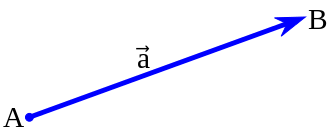
\includegraphics[scale=0.2]{pic/AB.png}
\quad
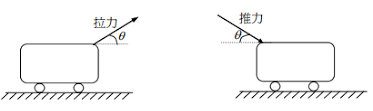
\includegraphics[scale=0.5]{pic/Force.png}
\ \\[10mm]
\pp
数学上的抽象总结:
\begin{center}
\framebox(300,50){ \LARGE \blue{向量} = 既有\underline{大小},又有\underline{方向}的量.}
\end{center}
\end{frame}





%\subsubsection{什么是向量}
%\begin{frame}\frametitle{向量的表达、模长、夹角}
%\begin{enumerate}
%	\item \blue{表达方式}:$\overset{\longrightarrow}{AB}$, $\vec{a}$, $\vec{b}$, $\vec{c}$, $\bf{a}$, $\bf{b}$, $\bf{c}$.
%	\item \blue{模长}: 向量的长度. 向量$\vec{a}$的模长记为$|\vec{a}|$.
%	\begin{itemize}
%		\item \blue{零向量}:$|\vec{a}|=0$. \blue{规定}任意方向都为零向量的方向.
%		\item \blue{单位向量}:$|\vec{a}|=1$.
%	\end{itemize}
%	\item \blue{相等}:大小相同,方向相同. 记为: $\vec{a}=\vec{b}$.\\
%\begin{equation*}
%\begin{tikzpicture}[scale=1]
%\tikzmath{\r=3;};
%\tikzmath{\R=5.5;};
%\coordinate (O) at (0,0);
%\coordinate (A) at (1,2);
%\coordinate (B) at (2,1);
%\draw[->,thick,blue](O)--(A) node[pos=.5,sloped,above] {$\vec{a}$};
%\draw[->,thick,red](O)--(B) node[pos=.5,sloped,above] {$\vec{b}$};
%\pp
%\coordinate (o) at (0+\r,0);
%\coordinate (a) at (1+\r,2);
%\coordinate (b) at (0.5+\r,1);
%\draw[->,thick,blue](o)--(a) node[pos=.5,sloped,above] {$\vec{a}$};
%\draw[->,red](o)--(b) node[pos=.5,sloped,above] {$\vec{b}$};
%\pp
%\coordinate (oo) at (0+\R,0);
%\coordinate (cc) at (1+\R,0);
%\coordinate (aa) at (1+\R,2);
%\coordinate (bb) at (2+\R,2);
%\draw[->,thick,blue](oo)--(aa) node[pos=.5,sloped,above] {$\vec{a}$};
%\draw[->,red](cc)--(bb) node[pos=.5,sloped,above] {$\vec{b}$};
%\draw[dotted](oo)--(cc);
%\draw[dotted](bb)--(aa);
%\end{tikzpicture}
%\end{equation*}
%	\item \blue{反向量}(\blue{负向量}):大小相同,方向相反. 记为 $-\vec{a}$.
%	\item \blue{夹角} 
\includegraphics[scale=0.2]{angle.png} $0\leq \theta \leq \pi$.
%	\begin{itemize}
%		\item \blue{平行}($\theta=0$或$\pi$). 特别地,零向量与任意向量平行.
%		\item \blue{垂直}或\blue{正交}($\theta=\frac\pi2$).
%	\end{itemize}
%\end{enumerate}
%\end{frame}





\subsubsection{向量加法}
\begin{frame}\frametitle{向量加法}
\begin{center}
速度,力的合成 \quad $\xRightarrow{\text{用数学语言抽象化}}$ \quad 向量的加法
\end{center}
\pp
\begin{definition}[向量的加法---平行四边形法则或者三角形法则]
\begin{equation*}
\begin{tikzpicture}[scale=1]
\tikzmath{\r=4;};
\coordinate (O) at (0,0);
\coordinate (A) at (1,2);
\coordinate (B) at (1.5,-0.5);
\coordinate (C) at (2.5,1.5);

\coordinate (o) at (0+\r,0);
\coordinate (a) at (1+\r,2);
\coordinate (b) at (1.5+\r,-0.5);
\coordinate (c) at (2.5+\r,1.5);

\draw[->,thick,blue](O)--(A) node[pos=.5,sloped,above] {$\vec{a}$};
\draw[->,thick,red](O)--(B) node[pos=.5,sloped,above] {$\vec{b}$};
\pp
\draw[dotted](A)--(C);
\draw[dotted](B)--(C);
\pp
\draw[->,thick,purple](O)--(C) node[pos=.5,sloped,above] {$\vec{a}+\vec{b}$};
\pp
\draw[->,thick,blue](o)--(a) node[pos=.5,sloped,above] {$\vec{a}$};
\pp
\draw[->,thick,red](a)--(c) node[pos=.5,sloped,above] {$\vec{b}$};
\pp
\draw[->,thick,purple](o)--(c) node[pos=.5,sloped,above] {$\vec{a}+\vec{b}$};
\end{tikzpicture}
\end{equation*}
\end{definition}
\end{frame}





\subsubsection{向量加法的基本性质}
\begin{frame}\frametitle{向量加法的基本性质}
\begin{proposition}[向量加法的基本性质]
\pp
\begin{enumerate}
\item 加法交换律: $\vec{a}+\vec{b}=\vec{b}+\vec{a}$;
\pp
\item 加法结合律: $\vec{a}+(\vec{b}+\vec{c})=(\vec{a}+\vec{b})+\vec{c}$;
\pp
\item 存在零元: $\vec{a}+\vec{0}=\vec{a}=\vec{0}+\vec{a}$;
\pp
\item 存在负元: $\vec{a}+(-\vec{a})=\vec{0}=(-\vec{a})+\vec{a}$;
\pp
\end{enumerate}
\end{proposition}
\end{frame}



\subsubsection{向量减法}
\begin{frame}\frametitle{向量减法}
\begin{definition}[向量的减法]
\[\vec{a}-\vec{b}:=\vec{a}+(-\vec{b}).\]
%\footnote{注: 先定义负元,后定义减法.}
\end{definition}

\pp

\begin{equation*}
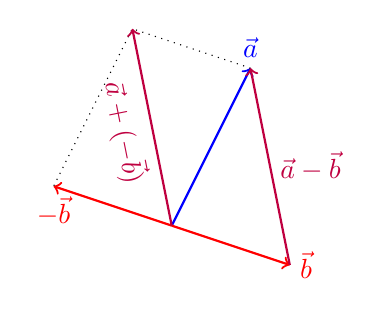
\begin{tikzpicture}[scale=1]
\coordinate (O) at (0,0);
\coordinate (A) at (1,2);
\coordinate (B) at (1.5,-0.5);
\coordinate (b) at (-1.5,0.5);
\coordinate (C) at (-0.5,2.5);
\pp
\draw[->,thick,blue](O)--(A) node[pos=1,above] {$\vec{a}$};
\draw[->,thick,red](O)--(B) node[pos=1,right] {$\vec{b}$};
\pp
\draw[->,thick,red](O)--(b) node[pos=1,below] {$-\vec{b}$};
\pp
\draw[dotted](A)--(C)--(b);
\pp
\draw[->,thick,purple](O)--(C) node[pos=0.5,sloped,below] {$\vec{a}+(-\vec{b})$};
\pp
\draw[->,thick,purple](B)--(A) node[pos=0.5,right] {$\vec{a}-\vec{b}$};
\end{tikzpicture}
\end{equation*}


\end{frame}





\subsubsection{向量的数乘}
\begin{frame}\frametitle{向量的数乘}
\begin{equation*}
\begin{tikzpicture}[scale=1]
\coordinate (O) at (0,0);\draw [fill] (O) circle [radius=0.03];
\coordinate (A) at (1,0);
\coordinate (05A) at (0.5*1,0);
\coordinate (2A) at (2*1,0);
\coordinate (mA) at (-1*1,0);
\coordinate (m15A) at (-1.5*1,0);
\coordinate (B) at (-1,1);
\coordinate (mpiB) at (3.14,-3.14);
\coordinate (eB) at (-2.718,2.718);
\draw[->,thick,blue](O)--(A) node[pos=1,sloped,below] {$\vec{a}$};
\pp
\draw[->,red](O)--(05A) node[pos=1,sloped,above] {$0.5\vec{a}$};
\pp
\draw[->,red](O)--(2A) node[pos=1,sloped,above] {$2\vec{a}$};
\pp
\draw[->,thick,green](O)--(mA) node[pos=1,sloped,below] {$-\vec{a}$};
\pp
\draw[->,purple](O)--(m15A) node[pos=1.2,sloped,above] {$-1.5\vec{a}$};
\pp
\draw[->,thick,blue](O)--(B) node[pos=1,above] {$\vec{b}$};
\draw[->,black](O)--(mpiB) node[pos=1,below] {$-\pi\vec{b}$};
\draw[->,black](O)--(eB) node[pos=1,above] {$e\vec{b}$};
\pp
\end{tikzpicture}
\end{equation*}
\end{frame}






\begin{frame}\frametitle{向量的数乘}
\begin{definition}[向量的数乘] 令$\vec{a}$为一向量, $\lambda$为一实数.\\
$\bullet$ 若$\lambda\geq0$,则$\lambda \vec{a}$定义为长度为$\lambda |\vec{a}|$且方向与$\vec{a}$相同的向量.\\
\pp
$\bullet$ 若$\lambda<0$,则$\lambda \vec{a}$定义为长度为$-\lambda |\vec{a}|$且方向与$\vec{a}$相反的向量.
\end{definition}
\pp

\textbf{记号}: 若 $\vec{a}\neq\vec{0}$,则记 $\blue{\vec{a}^0}:=\frac{1}{|\vec{a}|}\vec{a}$. 即, $\vec{a}^0$为方向与$\vec{a}$相同的\blue{单位向量}.
\pp

注：\blue{零向量}:$|\vec{a}|=0$. \blue{规定}任意方向都为零向量的方向.
\end{frame}





\subsubsection{向量数乘的基本性质}
\begin{frame}\frametitle{向量数乘的基本性质}
\begin{proposition}[向量数乘的基本性质]
\pp
\begin{enumerate}\setcounter{enumi}{4}
\item 数乘单位元: $1\vec{a} = \vec{a}$;
\pp
\item 数乘结合律: $\lambda(\mu \vec{a})=(\lambda \mu)\vec{a}$;
\pp
\item 左分配律: $(\lambda+\mu)\vec{a}=\lambda \vec{a} + \mu \vec{a}$;
\pp
\item 右分配律: $\lambda (\vec{a}+\vec{b}) =\lambda \vec{a} + \lambda \vec{b}$;
\end{enumerate}
\end{proposition}
\end{frame}





\subsubsection{线性运算}
\begin{frame}\frametitle{线性运算}
\begin{definition}[线性运算]
向量的\blue{加法}和\blue{数乘}运算统称为向量的\blue{线性运算}.
\end{definition}
\pp
\begin{proposition}[向量线性运算的八条基本性质]
\begin{enumerate}
\item 加法交换律: $\vec{a}+\vec{b}=\vec{b}+\vec{a}$;
\item 加法结合律: $\vec{a}+(\vec{b}+\vec{c})=(\vec{a}+\vec{b})+\vec{c}$;
\item 存在零元: $\vec{a}+\vec{0}=\vec{a}=\vec{0}+\vec{a}$;
\item 存在负元: $\vec{a}+(-\vec{a})=\vec{0}=(-\vec{a})+\vec{a}$;
\item 数乘单位元: $1\vec{a} = \vec{a}$;
\item 数乘结合律: $\lambda(\mu \vec{a})=(\lambda \mu)\vec{a}$;
\item 左分配律: $(\lambda+\mu)\vec{a}=\lambda \vec{a} + \mu \vec{a}$;
\item 右分配律: $\lambda (\vec{a}+\vec{b}) =\lambda \vec{a} + \lambda \vec{b}$;
\end{enumerate}
\end{proposition}
\pp
注：我们将通过这八条性质来公理化地定义一般的\blue{线性空间}或\blue{向量空间} (书本第五章,课件第六章).
\end{frame}





\subsection{向量线性相关性}





\subsubsection{线性组合}
\begin{frame}\frametitle{线性组合}
\begin{definition}[线性组合]
设 $\vec{a}_1$, $\vec{a}_2$, $\cdots$, $\vec{a}_m$  为一组向量, $\lambda_1$, $\lambda_2$, $\cdots$, $\lambda_m$ 为一组实数. 称向量
\[\lambda_1\vec{a}_1 + \lambda_2\vec{a}_2 + \cdots + \lambda_m\vec{a}_m\]
为向量 $\vec{a}_1$, $\vec{a}_2$, $\cdots$, $\vec{a}_m$ 的\blue{线性组合}.
\end{definition}
\pp
也就是说,一组向量的线性组合就是从这组向量出发通过线性运算能够获得的向量.
\pp
\begin{equation*}
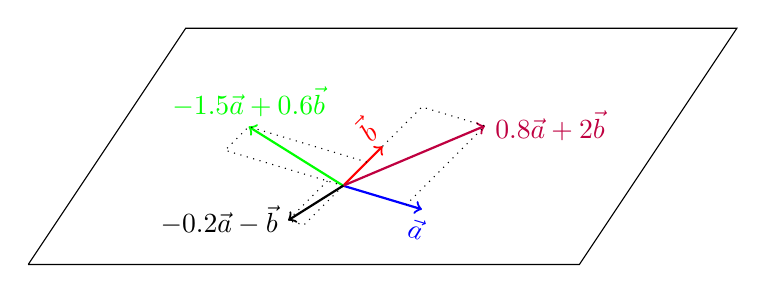
\begin{tikzpicture}[scale=1]
\coordinate (O) at (0,0);
\coordinate (A) at (1,-0.3);
\coordinate (B) at (0.5,0.5);
%---
\coordinate (08A) at (0.8,-0.24);
\coordinate (2B) at (1,1);
\coordinate (C1) at (1.8,0.76);   %0.8*(A)+2*(B);
%---
\coordinate (m15A) at (-1.5,0.45);
\coordinate (06B) at (0.3,0.3);
\coordinate (C2) at (-1.2,0.75);   %0.8*(A)+2*(B);
%---
\coordinate (m02A) at (-0.2,0.06);
\coordinate (mB) at (-0.5,-0.5);
\coordinate (C3) at (-0.7,-0.44);   %0.8*(A)+2*(B);
%---
\coordinate (D) at (-0.5,2.5);
\pp
\draw (-4,-1)--(-2,2)--(5,2)--(3,-1)--(-4,-1);
\draw[->,thick,blue](O)--(A) node[pos=1,sloped,below] {$\vec{a}$};
\draw[->,thick,red](O)--(B) node[pos=1,sloped,above] {$\vec{b}$};
\pp
\draw[->,thick,purple](O)--(C1) node[pos=1,right] {$0.8\vec{a}+2\vec{b}$};
\draw[dotted](B)--(2B)--(C1)--(08A);
\pp
\draw[->,thick,green](O)--(C2) node[pos=1,above] {$-1.5\vec{a}+0.6\vec{b}$};
\draw[dotted](06B)--(C2)--(m15A)--(O);
\pp
\draw[->,thick,black](O)--(C3) node[pos=1,left] {$-0.2\vec{a}-\vec{b}$};
\draw[dotted](m02A)--(C3)--(mB)--(O);
\end{tikzpicture}
\end{equation*}


\end{frame}


\subsubsection{线性组合的几何解释}
\begin{frame}\frametitle{线性组合的几何解释}

\begin{center}\blue{\framebox(300,50){
$\xymatrix@R=0mm@C=3cm{
\text{空间} \ar@{<->}[r]_-{\text{固定一个点$O$(原点)}}^-{1:1}& \text{全体向量集}\\
P \ar@{|->}[r] & \overset{\longrightarrow}{OP}\\
}$}}
\end{center}
\pp
\bigskip

\begin{enumerate}
\item 设 $\vec{a}$为一个非零向量。则
\begin{center}
过原点与 $\vec{a}$ 平行的\blue{直线} \quad $\xleftrightarrow{\quad 1:1 \quad}$ \quad $\vec{a}$的全体线性组合.
\end{center}
\pp
\bigskip


\item 设$\vec{a},\vec{b}$不平行(不共线). 则
\begin{center}
过原点与 $\vec{a}$ 和 $\vec{b}$ 平行的\blue{平面} \quad $\xleftrightarrow{\quad 1:1 \quad}$\quad  $\vec{a},\vec{b}$ 的全体线性组合.
\end{center}
\end{enumerate}

\pp
\bigskip

\red{这就是线性组合的威力:用少数几个向量表示特定子空间!}

\end{frame}








\subsubsection{线性相关与线性无关}
\begin{frame}\frametitle{线性相关与线性无关}
\begin{definition}[线性相关,线性无关] 给定一组向量 $\vec{a}_1$, $\vec{a}_2$, $\cdots$, $\vec{a}_m$.
\begin{itemize}
\item 如果存在一组不全为零的实数 $\lambda_1$, $\lambda_2$, $\cdots$, $\lambda_m$ 使得
\[\lambda_1\vec{a}_1 + \lambda_2\vec{a}_2 + \cdots + \lambda_m\vec{a}_m=\vec{0},\]
则称向量组$\vec{a}_1$, $\vec{a}_2$, $\cdots$, $\vec{a}_m$\blue{线性相关}.
\pp
\item 反之,若对任意一组不全为零的实数$\lambda_1$, $\lambda_2$, $\cdots$, $\lambda_m$都有
\[\lambda_1\vec{a}_1 + \lambda_2\vec{a}_2 + \cdots + \lambda_m\vec{a}_m\neq \vec{0},\]
则称向量组 $\vec{a}_1$, $\vec{a}_2$, $\cdots$, $\vec{a}_m$的\blue{线性无关}.
\end{itemize}
\end{definition}
\pp
\bigskip

特别地，设 $\vec{a}_1$, $\vec{a}_2$, $\cdots$, $\vec{a}_m$\blue{线性无关}. 若 $\lambda_1\vec{a}_1 + \lambda_2\vec{a}_2 + \cdots + \lambda_m\vec{a}_m= \vec{0}$, 则
$\lambda_1=\lambda_2= \cdots=\lambda_m=0$.

\pp
\bigskip

%\begin{example}
%向量组 \(\vec{a} = (1, 2, 3)\)，\(\vec{b} = (2, 3, 4)\)，\(\vec{c} = (3, 5, 7)\) 线性相关. 这是由于 \( \vec{a} +  \vec{b} - \vec{c} = \vec{0}\).
%\end{example}
%
%
%\begin{example}
%向量组 \(\vec{a} = (1, 0, 0)\)，\(\vec{b} = (0, 1, 0)\)，\(\vec{c} = (0, 0, 1)\) 线性无关. 假如线性相关, 则存在不全为零的实数 \(\lambda_1, \lambda_2, \lambda_3\) 使得
%\[\lambda_1 \vec{a} + \lambda_2 \vec{b} + \lambda_3 \vec{c} = \vec{0}\]
%即,
%   \[(\lambda_1, \lambda_2, \lambda_3) = (0, 0, 0)\]
%\end{example}



\begin{example}证明向量组$\vec{e}_1=\vec{a}+\vec{b}+\vec{c}$, $\vec{e}_2=\vec{a}-\vec{b}-\vec{c}$, $\vec{e}_3=\vec{a}+2\vec{b}+2\vec{c}$线性相关。
\end{example}

\pp

\red{$3\vec{e}_1 - \vec{e}_2 - 2\vec{e}_3 =\vec{0}$ 或 $\vec{e}_2 = 3\vec{e}_1-2\vec{e}_3$.}
\end{frame}





\subsubsection{线性相关的几何解释}
\begin{frame}\frametitle{线性相关的几何解释}
\begin{enumerate}
\item 一个向量$\vec{a}$线性相关 $\iff$ $\vec{a}=\vec0$;
\pp
\bigskip

\item 两个向量$\vec{a},\vec{b}$线性相关 $\iff$ $\vec{a}$与$\vec{b}$平行(共线);
\pp
\bigskip

\item 三个向量$\vec{a},\vec{b},\vec{c}$线性相关 $\iff$ $\vec{a},\vec{b},\vec{c}$共面;
\pp
\bigskip

\item 四个及四个以上的向量一定线性相关.
\end{enumerate}
\end{frame}








\subsection{坐标系、坐标与坐标变换}


\subsubsection{仿射坐标系}
\begin{frame}\frametitle{仿射坐标系}
为了推广笛卡尔坐标系到坐标轴不相互垂直的情形,
\begin{equation*}
\begin{tikzpicture}[scale=1]
\coordinate (o) at (0,0);
\coordinate (y) at (1,0);
\coordinate (x) at (-0.5,-0.5);
\coordinate (z) at (0,1);
\draw[->,thick,black](o)--(x) node[pos=1,below] {$x$};
\draw[->,thick,black](o)--(y) node[pos=1,right] {$y$};
\draw[->,thick,black](o)--(z) node[pos=1,above] {$z$};
\tkzMarkRightAngle(x,o,y)
\tkzMarkRightAngle(y,o,z)
\tkzMarkRightAngle(z,o,x)

\coordinate (O) at (4,0);
\node [below left] at (O) {$O$};
\coordinate (X) at (6,-1);
\coordinate (Y) at (5,0.5);
\coordinate (Z) at (3.5,1);
\draw[->,thick,black](O)--(X) node[pos=1,right] {$\vec{e}_1$};
\draw[->,thick,black](O)--(Y) node[pos=1,right] {$\vec{e}_2$};
\draw[->,thick,black](O)--(Z) node[pos=1,above] {$\vec{e}_3$};
\end{tikzpicture}
\end{equation*}
\pp
我们需要引入向量的基本定理.
\begin{theorem}[向量的基本定理]
设$\vec{e}_1$, $\vec{e}_2$, $\vec{e}_3$ 为空间中的三个不共面的向量, 则对每个向量$\vec{a}$都\blue{存在唯一}的三元有序实数组$(x_1,x_2,x_3)$, 使得
\[\vec{a} = x_1\vec{e}_1 + x_2\vec{e}_2 + x_3\vec{e}_3.\]
\end{theorem}
\end{frame}





\begin{frame}\frametitle{仿射坐标系}
\begin{definition}[基、坐标]
称不共面的三个向量$\vec{e}_1,\vec{e}_2,\vec{e}_3$为一组\blue{基}. 若
\[\vec{a} = x_1\vec{e}_1 + x_2\vec{e}_2 + x_3\vec{e}_3,\]
则称$(x_1,x_2,x_3)$为向量$\vec{a}$在基$\vec{e}_1,\vec{e}_2,\vec{e}_3$下的\blue{(仿射)坐标}.
\end{definition}
\pp
\begin{equation*}
\boxed{\blue{\text{仿射坐标系}}=\text{点} O  + \text{基} \vec{e}_1,\vec{e}_2,\vec{e}_3 \qquad \text{记作} \blue{[O;\vec{e}_1,\vec{e}_2,\vec{e}_3]}.}
\end{equation*}
\pp
%\blue{坐标原点}, \blue{坐标向量}, \blue{$x$轴}, \blue{$y$轴}, \blue{$z$轴}, \blue{坐标平面$Oxy$}, \blue{$Oyz$}, \blue{$Ozx$}.\\[2mm]
\begin{corollary}[一一对应]
若给定仿射坐标系 $[O;\vec{e}_1,\vec{e}_2,\vec{e}_3]$,则有如下一一对应
\begin{center}\blue{\framebox(300,50){
$\xymatrix@R=0mm{
\text{空间} \ar@{<->}[r]^-{1:1}& \text{全体向量集} \ar@{<->}[r]^-{1:1} & \mathbb R^3=\mathbb R\times \mathbb R \times \mathbb R \\
P \ar@{|->}[r] & \overset{\longrightarrow}{OP} \ar@{|->}[r] & \text{坐标}(x_1,x_2,x_3) \\
}$}}
\end{center}
\end{corollary}
\end{frame}





\subsubsection{向量的坐标运算}
\begin{frame}\frametitle{向量的坐标运算}
给定仿射坐标系 $[O;\vec{e}_1,\vec{e}_2,\vec{e}_3]$, 我们用$(x_1,x_2,x_3)$表示向量$x_1\vec{e}_1+x_2\vec{e}_2+x_3\vec{e}_3$.
\pp 则我们有
\begin{proposition}
$\bullet$ $(x_1,x_2,x_3) + (y_1,y_2,y_3) = (x_1+y_1,x_2+y_2,x_3+y_3)$;\\
\pp
$\bullet$ $\lambda(x_1,x_2,x_3) = (\lambda x_1,\lambda x_2,\lambda x_3)$.
\end{proposition}

\forppt{
\red{
\begin{equation*}
\begin{split}
(x_1,x_2,x_3) + (y_1,y_2,y_3) & := (x_1\vec{e}_1+x_2\vec{e}_2+x_3\vec{e}_3) + (y_1\vec{e}_1+y_2\vec{e}_2+y_3\vec{e}_3) \\
& = (x_1+y_1)\vec{e}_1 +(x_2+y_2)\vec{e}_2 +(x_3+y_3)\vec{e}_3 \\
& =: (x_1+y_1,x_2+y_2,x_3+y_3)\\
\lambda(x_1,x_2,x_3) & := \lambda (x_1\vec{e}_1+x_2\vec{e}_2+x_3\vec{e}_3) \\
& = \lambda x_1\vec{e}_1+\lambda x_2\vec{e}_2+\lambda x_3\vec{e}_3 \\
& =:  (\lambda x_1,\lambda x_2,\lambda x_3)\\
\end{split}
\end{equation*}
}}
\end{frame}








% ========== 2023年03月09号 第02次课 高维向量、数域、线性方程组 ==========




\subsubsection{坐标变换}
\begin{frame}\frametitle{坐标变换}
给定两个仿射坐标系 $[O;\vec{e}_1,\vec{e}_2,\vec{e}_3]$ 和 $[O';\vec{e}'_1,\vec{e}'_2,\vec{e}'_3]$.
\pp
\begin{question}
设空间中的点$P$在两个坐标系下的坐标分别为 $(x,y,z)$ 和 $(x',y',z')$. 求两个坐标之间的关系式？
\end{question}
\pp
为了回答这一问题，我们需要给出两个坐标系之间的位置关系:
\pp
\begin{itemize}
\item 设$O$在$[O';\vec{e}'_1,\vec{e}'_2,\vec{e}'_3]$下的坐标为$(x_0',y_0',z_0')$. 即
\[\overset{\longrightarrow}{O'O} = x'_0\vec{e}'_1+ y'_0\vec{e}'_2 + z'_0\vec{e}'_3.\]
\item \pp  设$\vec{e}_j$在基$\vec{e}'_1,\vec{e}'_2,\vec{e}'_3$下的坐标为$(a_{1j},a_{2j},a_{3j})$.即
\[ \vec{e}_j = a_{1j}\vec{e}'_1+ a_{2j}\vec{e}'_2 + a_{3j}\vec{e}'_3.\]
\end{itemize}
\pp
然后$P$在两个坐标系下的坐标之间的关系式可写为\footnote{后续,通过矩阵乘法可简化为 \blue{$X'=AX+X_0'$}.}：
\begin{equation*}
\blue{\boxed{
\begin{split}
x' &= a_{11}x+a_{12}y+a_{13}z+x_0'\\
y' &= a_{21}x+a_{22}y+a_{23}z+y_0'\\
z' &= a_{31}x+a_{32}y+a_{33}z+z_0'\\
\end{split}
}}\qquad
\pp  \red{pf: \overset{\longrightarrow}{O'P} = \overset{\longrightarrow}{O'O}+\overset{\longrightarrow}{OP}.}
\end{equation*}
\end{frame}




%\renewcommand{\mydate}{2025年2月27日\ 第二次课}

%\frame{\date{第二次课}\titlepage}


\subsection{复数与数域}





\subsubsection{复数}
\begin{frame}\frametitle{复数}
\begin{equation*}
\boxed{\xymatrix@R=4mm{
&\fbox{\text{\tiny 复数的代数表示}} &\sqrt{-1} \ar@<-1mm>[d]\\
z \ar@{}[r]|{=} & \underline{x} \ar@{}[r]|+ & \underline{i\ y}\\
&{\text{实部} \atop \mathrm{Re}z}\ar[u]&{\text{虚部}\atop \mathrm{Im}z}\ar[u]\\}}
\end{equation*}
\pp

\begin{columns}[c]
\column{5cm}
\boxed{\begin{tikzpicture}
\filldraw[black] (0,0) circle (2pt) node[below left]{$O$};
\filldraw[black] (2,1) circle (1pt) node[below]{};
\filldraw[black] (2,0) circle (1pt) node[below]{};
\filldraw[black] (0,1) circle (1pt) node[below]{};
\draw[black, thick,->]  (0,-0.5) -- (0,3) node[black,right]{虚轴};
\draw[black, thick,->]  (-0.5,0) -- (4,0) node[black,right]{实轴};
\draw[black, thick,dotted]  (2,1) -- (2,0) node[black,below]{$x$};
\draw[black, thick,dotted]  (2,1) -- (0,1) node[black,left]{$y$};
\draw[black, thick,->]  (0,0) -- (2,1) node[black,right]{${P(x,y) \atop z=x+iy}$};
\node[black] at (3.5,2.5){复平面};
\node[black] at (2,3.2){\fbox{\tiny 复数的几何表示}};
\node[black] at (0.8,0.2){$\theta$};
\node[black] at (1,0.7){$r$};
\draw[black, thick,-]  (0.44,0) -- (0.4,0.2);
\end{tikzpicture}}
\column{5cm}
\pp
\begin{itemize}
\item \blue{模长}:  $|z|:=|\overset{\longrightarrow}{OP}|=\sqrt{x^2+y^2}$;
\item \blue{辐角}: 实轴沿逆时针方向旋转到$\overset{\longrightarrow}{OP}$的角度.
\item \blue{共轭}: $\overline{z}:=x-iy$.
\item \blue{三角表示}:\\ $z=r(\cos\theta+i\sin\theta)$.
\end{itemize}
\end{columns}
\end{frame}







\subsubsection{数域}
\begin{frame}\frametitle{数域}
复数域的任意子集称为\blue{数集}. 例如: $\mathbb N$, $\mathbb Z$, $\mathbb Q$, $\mathbb R$,$\mathbb C$, $\cdots$.
\pp
\begin{definition} 若数集$\mathbb F$至少包含两元素,且关于数的{\bf 加减乘除封闭},则称$\mathbb F$为\blue{数域}.
\end{definition}
\pp
\begin{example}[本课程中最常用的域]
有理数集$\mathbb Q$,实数集$\mathbb R$,和复数集$\mathbb C$均为数域.
\end{example}
注:$\mathbb N$, $\mathbb Z$不为数域.
\pp

\blue{为什么需要数域概念?}
\begin{itemize}
\item 向量的坐标可以是实数,也可以是复数;
\item 统一的数域概念让我们可以同时处理实向量和复向量;
\item 后面的线性空间理论建立在任意数域上.
\end{itemize}

\pp
\yang{注:\begin{enumerate}
\item $\mathbb Q[\sqrt{2}]=\{a+b\sqrt2\mid a,b\in\mathbb Q\}$也是数域,但本课程不作要求.
\item $\mathbb Q$ 为最小的数域. 即,若$\mathbb F$为数域,则$\mathbb Q\subseteq \mathbb F$.
\end{enumerate}}
\end{frame}





\subsection{数组向量}


\subsubsection{高维数组向量的定义}
\begin{frame}\frametitle{高维数组向量的定义}
设$\mathbb F$为数域, $n$为正整数.
\pp
\begin{definition}我们称一个由$n$个$\mathbb F$上的数$a_1,a_2,\cdots,a_n$组成的有序数组
\[\vec{a} := (a_1,\cdots,a_n)\]
为\blue{数域$\mathbb F$上的一个$n$维数组向量}.其中$a_i$称为$\vec{a}$的\blue{第$i$个分量}. 数域$\mathbb F$上$n$维数组向量全体记为 \blue{$\mathbb F^n$}.
\end{definition}
\pp
记法:
\begin{equation*}
\blue{\text{行向量:\ }} \vec{a} = (a_1,\cdots,a_n)\in \mathbb F^n \qquad \blue{\text{列向量:\ }} \vec{a}=\left(\begin{array}{c}a_1\\a_2\\\vdots\\a_n\\\end{array}\right)\in \mathbb F^n
\end{equation*}
\end{frame}




% ===== 新增:从三维到高维的过渡 =====
\subsubsection{从三维到高维}
\begin{frame}\frametitle{从三维到高维}
\begin{question}
三维空间中的向量有三个分量$(x,y,z)$. 那么四维、五维向量是什么?
\end{question}
\pp

\blue{例子1:时空向量(四维)}
\begin{itemize}
\item 相对论中,事件由时间和空间位置确定:$(t,x,y,z)$
\item 这是一个\blue{四维向量}!
\end{itemize}
\pp

\blue{例子2:颜色向量(三维或四维)}
\begin{itemize}
\item RGB颜色模型:$(R,G,B)$ (红、绿、蓝三个分量)
\item RGBA颜色模型:$(R,G,B,A)$ (增加透明度分量)
\end{itemize}
\pp

\blue{例子3:学生成绩向量(n维)}
\begin{itemize}
\item 一个学生的成绩可以表示为:$(\text{数学},\text{物理},\text{化学},\text{英语},\cdots)$
\item 如果有$n$门课,就是一个\blue{$n$维向量}!
\end{itemize}
\pp

\bigskip

\begin{center}
\framebox{\blue{向量的维数 = 描述对象所需的独立参数个数 = 自由度}}
\end{center}
\end{frame}

\subsubsection{高维向量的应用}
\begin{frame}\frametitle{高维向量的应用}
\begin{example}[机器学习中的特征向量]
要识别一张图片是否包含猫,需要提取图片的特征:
\begin{itemize}
\item 颜色直方图(256维)
\item 边缘特征(128维)
\item 纹理特征(64维)
\item $\cdots$
\end{itemize}
\pp
最终得到一个\blue{几千维的向量}来表示这张图片!
\end{example}
\pp

\begin{example}[推荐系统中的用户向量]
一个用户对$n$部电影的评分可以表示为一个$n$维向量:
\[(r_1,r_2,\cdots,r_n)\]
其中$r_i$是用户对第$i$部电影的评分。
\end{example}

\end{frame}

\begin{frame}\frametitle{大模型中的高维向量}

\begin{example}[DeepSeek-V3]
设 $T$ 是 DeepSeek-V3 的 token 词表,  $|T|=129280$. \pp 词嵌入给每个 token 分配一个 7168 维向量：
\[E \colon  T \longrightarrow \mathbb R^{7168}.\]
\pp
为了储存映射 $E$, 我们需要
\[129208 \times 7168 = 926679040\]
个参数。
\pp
这约 9.27 亿个参数最初随机初始化, 之后与整个模型一起训练; 这些向量不是人工规定的,而是从大量语言数据中学习出来的.
\end{example}


\red{高维向量在现代科学和工程中无处不在!}

\end{frame}

% ===== 原有的高维数组向量定义(652-693行) =====




\subsubsection{高维数组向量的线性运算}
\begin{frame}\frametitle{高维数组向量的线性运算}
设 $\vec{a}=(a_1,\cdots,a_n)\in \mathbb F^n$, $\vec{b}=(b_1,\cdots,b_n)\in \mathbb F^n$, $\lambda\in \mathbb F$.
\begin{enumerate}[]
\item 加法: $\vec{a}+\vec{b}:=(a_1+b_1,a_2+b_2,\cdots,a_n+b_n)$.
\pp
\item 数乘: $\lambda \vec{a}:=(\lambda a_1,\lambda a_2,\cdots,\lambda a_n)$.
\pp
\item 零向量: $\vec{0}:=(0,\cdots,0)$.
\item 负向量: $-\vec{a}:=(-a_1,\cdots,-a_n)$.
\item 相等: $\vec{a}=\vec{b} \iff a_i=b_i \quad i=1,\cdots,n$.
\end{enumerate}
\pp
\blue{八条基本性质:}
\begin{enumerate}
\item 加法交换律: $\vec{a}+\vec{b}=\vec{b}+\vec{a}$;
\item 加法结合律: $\vec{a}+(\vec{b}+\vec{c})=(\vec{a}+\vec{b})+\vec{c}$;
\item 存在零元: $\vec{a}+\vec{0}=\vec{a}=\vec{0}+\vec{a}$;
\item 存在负元: $\vec{a}+(-\vec{a})=\vec{0}=(-\vec{a})+\vec{a}$;
\item 数乘单位元: $1\vec{a} = \vec{a}$;
\item 数乘结合律: $\lambda(\mu \vec{a})=(\lambda \mu)\vec{a}$;
\item 左分配律: $(\lambda+\mu)\vec{a}=\lambda \vec{a} + \mu \vec{a}$;
\item 右分配律: $\lambda (\vec{a}+\vec{b}) =\lambda \vec{a} + \lambda \vec{b}$;
\end{enumerate}
\end{frame}




\subsubsection{线性相关(高维数组向量)}
\begin{frame}\frametitle{线性相关(高维数组向量)}
设$\vec{a}_1,\vec{a}_2,\cdots,\vec{a}_m\in \mathbb F^n$,  $\lambda_1,\lambda_2,\cdots,\lambda_m\in \mathbb F$.
\begin{center}
\fbox{\blue{$\lambda_1\vec{a}_1 + \lambda_2\vec{a}_2 + \cdots + \lambda_m\vec{a}_m$} \qquad $\longleftarrow$ \blue{线性组合} }
\end{center}
\pp
\begin{definition}[线性相关,线性无关]
一组向量 $\vec{a}_1$, $\vec{a}_2$, $\cdots$, $\vec{a}_m$ 称为\blue{线性相关}, 若存在一组不全为零的 $\mathbb F$ 中的数  $\lambda_1$, $\lambda_2$, $\cdots$, $\lambda_m$ 使得
\[\lambda_1\vec{a}_1 + \lambda_2\vec{a}_2 + \cdots + \lambda_m\vec{a}_m=0.\]
反之,	则称向量 $\vec{a}_1$, $\vec{a}_2$, $\cdots$, $\vec{a}_m$的\blue{线性无关}.
\end{definition}
\end{frame}





\begin{frame}
\begin{example} 记 $\vec{e}_1=(1,0,\cdots,0)$, $\vec{e}_2=(0,1,\cdots,0)$, $\cdots$, $\vec{e}_n=(0,0,\cdots,1)$. 则$\vec{e}_1,\vec{e}_2,\cdots,\vec{e}_n$线性无关. 称这$n$个向量为\blue{基本向量}.
\end{example}
\pp

\begin{fact}
基本向量线性无关，且任意$n$维数组向量都可以表示为基本向量的线性组合.
\[\begin{pmatrix}x_1\\x_2\\\vdots\\x_n\end{pmatrix} = x_1\vec{e}_1+x_2\vec{e}_2+\cdots+x_n\vec{e}_n.\]
\end{fact}

\end{frame}


\subsubsection{本章主要内容}
\begin{frame}\frametitle{本章主要内容}

\begin{equation*}
\xymatrix@R=0.5cm@C=0.5cm{
\text{空间向量} \ar[d] &\\
\text{线性运算} \ar[d]&\\
\text{线性组合} \ar[d] \ar[dr] &\\
\text{线性相关性} \ar[r]  & \text{仿射坐标系} \ar[r] & \text{坐标}\ar[d]\ar[r] & \text{坐标变换}   \\
\text{复数}\ar[r] &\text{数域} \ar[r] & \text{数组向量} \ar[d]\\
\text{线性相关性}\ar[d] & \text{线性组合} \ar[l] & \text{数组向量的线性运算} \ar[l]\\
\text{基本向量}&
}
\end{equation*}
\end{frame}










%\subsection{求和号}
%
%
%\subsubsection{什么是向量}
%\begin{frame}\frametitle{求和号}
%\forhandout{本小节留给助教习题课讲解?}
%
%\[\sum_{i=1}^n a_i:= a_1 + a_2 + \cdots + a_n\]
%\pp
%\begin{proposition}
%\[\sum_{i=1}^n (a_i+b_i) = \sum_{i=1}^n a_i + \sum_{i=1}^n b_i; \qquad \sum_{i=1}^n \lambda a_i = \lambda\sum_{i=1}^n a_i\]
%\end{proposition}
%\end{frame}
%
%
%
%
%\subsubsection{什么是向量}
%\begin{frame}\frametitle{多重求和号}
%\begin{equation*}
%\begin{split}
%\sum_{j=1}^{m}\sum_{i=1}^{n} a_{ij} & := \sum_{j=1}^{m}\left(a_{1j}+a_{2j}+\cdots+a_{nj}\right)\\
%\end{split}
%\end{equation*}
%\begin{equation*}
%\begin{split}
%\sum_{i=1}^{n}\sum_{j=1}^{m} a_{ij} & := \sum_{i=1}^{n}\left(a_{i1}+a_{i2}+\cdots+a_{im}\right)\\
%\end{split}
%\end{equation*}
%\pp
%\begin{proposition}
%\[\sum_{j=1}^m\sum_{i=1}^na_{ij} = \sum_{i=1}^n\sum_{j=1}^ma_{ij}.\]
%有时候,将这一值简记为 $\sum\limits_{1\leq i,j\leq n} a_{ij}$.
%\end{proposition}
%
%\end{frame}
%
%
%
%
%
%
%
%\subsubsection{什么是向量}
%\begin{frame}\frametitle{条件求和}
%
%\[\sum_{1\leq i\leq j\leq n} a_{ij}:= a_{11} + (a_{12} + a_{22}) + \cdots+ (a_{1n}+a_{2n}+\cdots+a_{nn}).\]
%\pp
%\begin{proposition}
%\[\sum_{1\leq i\leq j\leq n} a_{ij} = \sum_{j=1}^n\sum_{i=1}^j a_{ij} = \sum_{i=1}^n\sum_{j=i}^n a_{ij}.\]
%\end{proposition}
%\pp
%\begin{example}
%\[\sum_{i=1}^{n}\sum_{j=1}^{m}a_ib_j = \left(\sum_{i=1}^{n} a_i\right)\left(\sum_{j=1}^{m} b_j\right).\]
%\end{example}
%\end{frame}


%================================================
%\setcounter{framenumber}{30}
\renewcommand{\mydate}{2025年2月27号 第二次课}
\makeatletter
\ifodd\value{page}
\else
\begin{frame}[plain]\end{frame}
\fi
\makeatother
%================================================
%================================================
\section{线性方程组}
\title{第二章 \quad 线性方程组}
\author{}
\date{}
%================================================
%================================================
\frame{\titlepage}
%================================================
%================================================

\subsection{概念和基本问题}


\subsubsection{研究对象}
\begin{frame}\frametitle{研究对象}
\begin{enumerate}
\item 小学(鸡兔同笼) \\
\begin{columns}
\begin{column}{0.6\textwidth}
\begin{center}今有雉兔同笼，\\上有三十五头，\\下有九十四足，\\问雉兔各几何？\\\end{center}
\end{column}
\begin{column}{0.3\textwidth}
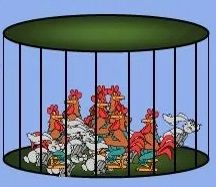
\includegraphics[scale=0.3]{pic/鸡兔同笼.jpg}
\end{column}
\end{columns} \pp
\item 初中(二元一次方程组)\\
\begin{equation*}
\left\{\begin{array}{rrrrrrr}
x& +& y &= & 35 && \\
2x& + & 4y& = & 94 && \\
\end{array}\right.
\end{equation*} \pp
\item 现在(\blue{线性方程组}：即,\textbf{任意个变量}及\textbf{任意个方程}构成的\textbf{一次}方程组.)\\
%\begin{equation}
%\left\{\begin{array}{ccccccccc}
%	a_{11}x_1& +& a_{12}x_2 & + & \cdots & + & a_{1n}x_n &= & b_1\\
%	a_{21}x_1& +& a_{22}x_2 & + & \cdots & + & a_{2n}x_n &= & b_2\\
%	\vdots && 	\vdots && 	\ddots && 	\vdots && 	\vdots \\
%	a_{m1}x_1& +& a_{m2}x_2 & + & \cdots & + & a_{mn}x_n &= & b_m\\
%\end{array}\right.
%\end{equation}
\end{enumerate}
\end{frame}







\subsubsection{线性方程组}
\begin{frame}\frametitle{线性方程组}
\begin{equation} \label{system_of_linear_equations}\tag{$*$}
\left\{\begin{array}{ccccccccc}
a_{11}x_1& +& a_{12}x_2 & + & \cdots & + & a_{1n}x_n &= & b_1\\
a_{21}x_1& +& a_{22}x_2 & + & \cdots & + & a_{2n}x_n &= & b_2\\
\vdots && 	\vdots && 	\ddots && 	\vdots && 	\vdots \\
a_{m1}x_1& +& a_{m2}x_2 & + & \cdots & + & a_{mn}x_n &= & b_m\\
\end{array}\right.
\end{equation} \pp
\begin{enumerate}
\item $x_j$: 第$j$个\blue{变量} \pp
\item $a_{ij}$:  第$i$个方程第$j$个变量$x_j$的\blue{系数}; \pp
\item $b_i$:  第$i$个方程的\blue{常数项}. \pp
\item 如果$b_1 = \cdots = b_m =0$, 则称方程组\eqref{system_of_linear_equations}为\blue{齐次线性方程组}。否则称之为\blue{非齐次线性方程组}。
\end{enumerate} \pp
\begin{example}
\setlength{\arraycolsep}{0.5pt}
$\left\{\begin{array}{rrrrrrr}
x& +& y &= & 0 && \\
2x& + & 4y& = & 0 && \\
\end{array}\right.(\text{齐次})
\qquad \pp
\left\{\begin{array}{rrrrrrr}
x& +& y &= & 35 && \\
2x& + & 4y& = & 94 && \\
\end{array}\right.(\text{非齐次})$
\end{example}
\end{frame}





\subsubsection{线性方程组的解}
\begin{frame}\frametitle{线性方程组的解}
\begin{enumerate}
\item 令$c_1,\cdots,c_n$为一组数。若将$x_1=c_1$，$\cdots$，$x_n=c_n$代入方程组\eqref{system_of_linear_equations}，等式都成立，则称$(c_1,\cdots,c_n)$为\blue{一组解}。\pp 称有所有解组成的集合为\blue{解集}。 \pp
\item 如果解集非空，我们称方程组\eqref{system_of_linear_equations}是\blue{相容的}，否则称之为\blue{不相容的}。 \pp
\end{enumerate}
\begin{example}线性方程组 $\left\{\begin{array}{rrrrrrr}
x& +& y &= & 35 && \\
2x& + & 4y& = & 94 && \\
\end{array}\right.$是相容，因为二元数组$(23,12)$为它的一组解。通过初等计算验证，可以得出这一方程组的解集正好为$\{(23,12)\}$.
\end{example}
\end{frame}





\subsubsection{关于线性方程组的几个基本问题}
\begin{frame}\frametitle{关于线性方程组的几个基本问题}
\begin{enumerate}
\item 解是否存在，是否唯一？ \pp
\item 如何求解？\pp
\item 解集的公式表达。 \pp
\item 解集的几何结构。\pp
\end{enumerate}

注：\begin{enumerate}
\item[$\bullet$] 前两个问题可以用\blue{Gauss消元法}解决(本次课的主要内容)。 \pp
\item[$\bullet$] 后两个问题需要用\blue{矩阵}、\blue{行列式}和\blue{线性空间}等基本工具与研究对象(书本第四五章的主要内容)。
\end{enumerate}
\end{frame}





\subsection{Gauss 消元法}


\subsubsection{Gauss消元法}
\begin{frame}\frametitle{Gauss消元法}
\begin{example}[鸡兔同笼]
求解 $\left\{\begin{array}{rrrrrrr}
x& +& y &= & 35 && (1) \\
2x& + & 4y& = & 94 && (2)\\
\end{array}\right.$.
\end{example}
\pp
\bigskip

解：
第一步, 方程(2)减去两倍的方程(1)得
\[\xrightarrow{\blue{-2(1)\rightarrow(2)}} \left\{\begin{array}{rrrrrrr}
x& +& y &= & 35 && (3) \\
&  & \red{2}y& = & 24 && (4)\\
\end{array}\right.\]
\pp
\bigskip

第二步, 方程(4)除以$2$
\[\xrightarrow{\blue{\frac12(4)}}\left\{\begin{array}{rrrrrrr}
x& \red{+}& y &= & 35 && (5) \\
&  & y& = & 12 && (6)\\
\end{array}\right.\]
\pp
\bigskip

第三步. 方程(5)减去方程(6)
\[\xrightarrow{-(6)\rightarrow(5)}\left\{\begin{array}{rrrrrrr}
x& & &= & 23 && \\
&  & y& = & 12 &&\\
\end{array}\right.\]
\end{frame}





\begin{frame}\frametitle{Gauss 消元法}
\begin{example}
求解 $\left\{\begin{array}{rrrrrrrrr}
3x_1 & + & 2x_2 & - & x_3 & = & 6 && (1)\\
x_1 & + & 3x_2 & + & 2x_3 & = & 9 && (2)\\
2x_1 & - & x_2 & + & 3x_3 & = & 3 && (3)\\
\end{array}\right.$.
\end{example}
\pp
\bigskip

解：交换前两个方程的顺序\\[2mm]
{ $\xrightarrow{\blue{(1)\leftrightarrow(2)}}\left\{\begin{array}{rrrrrr}
x_1 & +3x_2 & +2x_3 & =&9 & (4)\\
\red{3}x_1 &+2x_2 & -x_3 & =& 6 & (5)\\
\red{2}x_1 & -x_2 & +3x_3 & =&3 & (6)\\
\end{array}\right. $} \\[2mm]
\pp
\bigskip

{ $\xrightarrow[-2(4)\rightarrow (6)]{-3(4)\rightarrow(5)}\left\{\begin{array}{rrrrrr}
x_1 & +3x_2 & +2x_3 & =& 9 & (7)\\
& -7x_2 & -7x_3 & =& -21 & (8)\\
& \red{-7}x_2 &  -x_3 & =& -15 & (9)\\
\end{array}\right. $}\\[2mm]
\pp
\bigskip

{ $\xrightarrow{-(8)\rightarrow(9)}\left\{\begin{array}{rrrrrr}
x_1 & +3x_2 & +2x_3 & =& 9 & (10)\\
& -7x_2 & -7x_3 & =& -21 & (11)\\
&       &  \red{6}x_3 & =&   6 & (12)\\
\end{array}\right. $}
\end{frame}





\begin{frame}\frametitle{}
{ $\xrightarrow{\frac16(12)}\left\{\begin{array}{rrrrrr}
x_1 & +3x_2 & +2x_3 & =&   9 & (13)\\
& -7x_2 & \red{-7}x_3 & =& -21 & (14)\\
&       &  x_3 & =&   1 & (15)\\
\end{array}\right. $}\\[2mm]
\pp
\bigskip

{ $\xrightarrow{7(15)\rightarrow(14)}\left\{\begin{array}{rrrrrr}
x_1 & +3x_2 & +2x_3 & =&   9 & (16)\\
& \red{-7}x_2 &      & =& -14 & (17)\\
&       &  x_3 & =&   1 & (18)\\
\end{array}\right. $} \\[2mm]
\pp
\bigskip

{ $\xrightarrow{-\frac17(14)}\left\{\begin{array}{rrrrrr}
x_1 & \red{+3}x_2 & \red{+2}x_3  & =&   9 & (19)\\
& x_2 &         &   =& 2 & (20)\\
&       &  x_3 & =&   1 & (21)\\
\end{array}\right. $}\\[2mm]
\pp
\bigskip

{$\xrightarrow[-2(21)\rightarrow (19)]{-3(20)\rightarrow (19)}\left\{\begin{array}{rr}
x_1 =&   1\\
x_2 =& 2 \\
x_3 =&   1\\
\end{array}\right. $ \pp
(代回验证，成立） $\Rightarrow$ 解集为$\{(1,2,1)\}$.}
\end{frame}





\subsubsection{方程的三种初等变换}
\begin{frame}\frametitle{方程的三种初等变换}
\begin{tabular}{r||l|r}
&初等变换 & 记号\\\hline\hline
(1) & 交换两个方程 & $(i)\leftrightarrow(j)$\\\hline
(2) & 某个方程乘以一个非零常数 & $\lambda(i)$\\\hline
(3) & 某个方程乘一个常数加到另一个方程上 & $\lambda(i)\rightarrow (j)$\\
\end{tabular}
\end{frame}





\begin{frame}
\begin{example}[存在不唯一]
求解 $\left\{\begin{array}{rrrrrrr}
x_1 & +2x_2 & +3x_3 &  +4x_4 & = & -3 &  \qquad (1)\\
x_1 & +2x_2 &       &  -5x_4 & = &  1 &  \qquad (2)\\
2x_1 & +4x_2 & -3x_3 & -19x_4 & = &  6 &  \qquad (3)\\
3x_1 & +6x_2 & -3x_3 & -24x_4 & = &  7 &  \qquad (4)\\
\end{array}\right.$
\end{example} \pp
{\tiny 解：\\
$\xrightarrow[-3(1)\rightarrow(4)]{- 1(1)\rightarrow(2) \atop -2(1)\rightarrow(3)}
\left\{\begin{array}{rrrrrrr}
x_1 & +2x_2 & \red{+3}x_3 &  +4x_4 & = &  -3 &    (5)\\
&       & -3x_3 &  -9x_4 & = &   4 &    (6)\\
&       & \red{-9}x_3 & -27x_4 & = &  12 &    (7)\\
&       &\red{-12}x_3 & -36x_4 & = &  16 &    (8)\\
\end{array}\right.
$ \pp
\bigskip

$\xrightarrow[-4(6)\rightarrow(8)]{(6)\rightarrow(5)\atop -3(6)\rightarrow(7)}
\left\{\begin{array}{rrrrrrr}
x_1 & +2x_2 &  &  -5x_4 & = &  1 &    (9)\\
&       & \red{-3}x_3 &  -9x_4 & = &   4 &    (10)\\
&       &       &      0 & = &  0 &    (11)\\
&       &       &      0 & = &  0 &    (12)\\
\end{array}\right.
$ \pp
\bigskip

$\xrightarrow{-\frac13(10)}
\left\{\begin{array}{rrrrrrr}
x_1 & +2x_2 &  &  -5x_4 & = &  1 &    (13)\\
&       & x_3 &  +3x_4 & = &   -\frac43 &    (14)\\
&       &       &      0 & = &  0 &    (15)\\
&       &       &      0 & = &  0 &    (16)\\
\end{array}\right.
$ \pp
$\Rightarrow \left\{
\begin{array}{rl}
x_1 &= 1-2x_2+5x_4\\
x_3 &= -\frac43 - 3x_4\\
\end{array}
\right.$
\\ \pp
\bigskip

因此$x_2$和$x_4$可取任意值，$x_1$和$x_3$由$x_2$和$x_4$的取值唯一确定。\pp 即，
\[\left\{
\begin{array}{rl}
x_1 &= 1-2t_1+5t_2\\
x_2 &= t_1 \\
x_3 &= -\frac43 - 3t_2\\
x_4 &= t_2 \\
\end{array}
\right. \qquad \text{其中} t_1,t_2\in \bF.\]
}
\end{frame}









% ========== 2023年03月14号 第03次课 线性方程组、矩阵 ==========
%\frame{\titlepage}





\begin{frame}

\begin{example}[解存在且唯一]
求解 $\left\{\begin{array}{rrrrrrr}
x& +& y &= & 35 && (1) \\
2x& + & 4y& = & 94 && (2)\\
\end{array}\right.$.
\end{example}

\[\Rightarrow \left\{\begin{array}{rrrrrrr}
x& & &= & 23 && \\
&  & y& = & 12 &&\\
\end{array}\right.\]
\begin{example}[解存在但不唯一]
求解 $\left\{\begin{array}{rrrrrrr}
x_1 & +2x_2 & +3x_3 &  +4x_4 & = & -3 &  \qquad (1)\\
x_1 & +2x_2 &       &  -5x_4 & = &  1 &  \qquad (2)\\
2x_1 & +4x_2 & -3x_3 & -19x_4 & = &  6 &  \qquad (3)\\
3x_1 & +6x_2 & -3x_3 & -24x_4 & = &  7 &  \qquad (4)\\
\end{array}\right.$
\end{example}
\[\Rightarrow \left\{
\begin{array}{rl}
x_1 &= 1-2t_1+5t_2\\
x_2 &= t_1 \\
x_3 &= -\frac43 - 3t_2\\
x_4 &= t_2 \\
\end{array}
\right. \qquad \text{其中} t_1,t_2\in \mathbb F.\]
\end{frame}





\begin{frame}
\begin{example}[无解]
求解 $\left\{\begin{array}{rrrrrrr}
x_1 &  -x_2 & +x_3 & = & 1 &  \qquad (1)\\
x_1 &  -x_2 & -x_3 & = & 3 &  \qquad (2)\\
2x_1 & -2x_2 & -x_3 & = & 3 &  \qquad (3)\\
\end{array}\right.$
\end{example} \pp
{解：\\
$\xrightarrow[-2(1)\rightarrow(3)]{-1(1)\rightarrow(2)}
\left\{\begin{array}{rrrrrrr}
x_1 &  -x_2 & +x_3 & = & 1 &   (4)\\
&  & -2x_3 & = & 2 & (5)\\
&  & -3x_3 & = & 1 & (6)\\
\end{array}\right.$ \pp
\bigskip

$\xrightarrow[-\frac32(5)\rightarrow(6)]{\frac12(5)\rightarrow(4)}
\left\{\begin{array}{rrrrrrr}
x_1 &  -x_2 &  & = & 2 & \\
&  & -2x_3 & = & 2 & \\
&  & \red{0} & \red{=} & \red{-2} & \\
\end{array}\right.$ \pp
\bigskip

\[\Rightarrow \textbf{无解！！}\]
}
\end{frame}





\begin{frame}
我们称有相同的解集的两个线性方程组互为对方的\blue{同解方程组}. \pp
\begin{theorem}
三种初等变换将线性方程组变为同解线性方程组.
\end{theorem} \pp
\begin{proof} \tiny
这里只给出第三种初等变换的证明，其他两种情形证明类似。\pp
\begin{equation*}
\setlength{\arraycolsep}{0.5pt}
\left\{\begin{array}{ccccccccc}
a_{11}x_1& + & \cdots & + & a_{1n}x_n &= & b_1\\
\vdots & & 	\ddots && 	\vdots && 	\vdots \\
a_{i1}x_1& + & \cdots & + & a_{in}x_n &= & b_i\\
\vdots && 	\ddots && 	\vdots && 	\vdots \\
a_{j1}x_1& + & \cdots & + & a_{jn}x_n &= & b_j\\
\vdots && 	\ddots && 	\vdots && 	\vdots \\
a_{m1}x_1& + & \cdots & + & a_{mn}x_n &= & b_m\\
\end{array}\right.
\xrightleftharpoons[-\lambda(i)\rightarrow(j)]{\lambda(i)\rightarrow(j)}
\left\{\begin{array}{ccccccccc}
a_{11}x_1&+ & \cdots & + & a_{1n}x_n &= & b_1\\
\vdots && 	\ddots && 	\vdots && 	\vdots \\
a_{i1}x_1&+ & \cdots & + & a_{in}x_n &= & b_i\\
\vdots && 	\ddots && 	\vdots && 	\vdots \\
(a_{j1}+\lambda a_{i1})x_1& + & \cdots & + & (a_{jn}+\lambda a_{in})x_n &= & b_j+\lambda b_i\\
\vdots && 	\ddots && 	\vdots && 	\vdots \\
a_{m1}x_1& + & \cdots & + & a_{mn}x_n &= & b_m\\
\end{array}\right.
\end{equation*}
\end{proof}
\end{frame}









\subsection{Gauss消元法的矩阵表示}


\subsubsection{矩阵}
\begin{frame}\frametitle{矩阵}
\begin{definition}
我们称由若干行及若干列的数组成的阵列为\blue{矩阵}.
\end{definition} \pp
\bigskip

例如: 线性方程组
\begin{equation*} \tag{$*$}
\left\{\begin{array}{ccccccccc}
a_{11}x_1& +& a_{12}x_2 & + & \cdots & + & a_{1n}x_n &= & b_1\\
a_{21}x_1& +& a_{22}x_2 & + & \cdots & + & a_{2n}x_n &= & b_2\\
\vdots && 	\vdots && 	\ddots && 	\vdots && 	\vdots \\
a_{m1}x_1& +& a_{m2}x_2 & + & \cdots & + & a_{mn}x_n &= & b_m\\
\end{array}\right.
\end{equation*}

的系数和常数项组成一个矩阵
\begin{equation*}
\left(\begin{array}{ccccc}
a_{11} & a_{12} & \cdots & a_{1n} & b_1 \\
a_{21} & a_{22} & \cdots & a_{2n} & b_2 \\
\vdots & \vdots & \ddots & \vdots & \vdots\\
a_{m1} & a_{m2} & \cdots & a_{mn} & b_m \\
\end{array}\right) \qquad \text{$\longleftarrow$ 方程组 $(*)$ 的\blue{增广矩阵} }
\end{equation*}
\pp
\bigskip

\textbf{注：}由于变元不参与运算，因此可以用增广矩阵来表示方程组。
\end{frame}




\subsubsection{Gauss消元法的矩阵表示}
\begin{frame}\frametitle{Gauss消元法的矩阵表示}
\begin{example}[非齐次线性方程组]
求解 $\left\{\begin{array}{rrrrrrrrr}
3x_1 & + & 2x_2 & - & x_3 & = & 6 \\
x_1 & + & 3x_2 & + & 2x_3 & = & 9 \\
2x_1 & - & x_2 & + & 3x_3 & = & 3\\
\end{array}\right.$.
\end{example}
\pp
{解：\small {
$\left(\begin{array}{rrrr}3&2&-1&6\\1&3&2&9\\2&-1&3&3\\\end{array}\right)$ \pp
$\xrightarrow{r_1\leftrightarrow r_2}$
$\left(\begin{array}{rrrr}1&3&2&9\\3&2&-1&6\\2&-1&3&3\\\end{array}\right)$
\pp
\bigskip

$\xrightarrow[-2r_1\rightarrow r_3]{-3r_1\rightarrow r_2}$
$\left(\begin{array}{rrrr}1&3&2&9\\0&-7&-7&-21\\0&-7&-1&-15\\\end{array}\right)$ \pp
$\xrightarrow{-r_2\rightarrow r_3}$
$\left(\begin{array}{rrrr}1&3&2&9\\0&-7&-7&-21\\0&0&6&6\\\end{array}\right)$
\pp
\bigskip

$\xrightarrow{\frac16r_3}$
$\left(\begin{array}{rrrr}1&3&2&9\\0&-7&-7&-21\\0&0&1&1\\\end{array}\right)$ \pp
$\xrightarrow[-2r_3\rightarrow r_1]{7r_3\rightarrow r_2}$
$\left(\begin{array}{rrrr}1&3&0&7\\0&-7&0&-14\\0&0&1&1\\\end{array}\right)$	 \pp
\bigskip

$\xrightarrow[\frac37r_2\rightarrow r_1]{-\frac17r_2}$
$\left(\begin{array}{rrrr}1&0&0&1\\0&1&0&2\\0&0&1&1\\\end{array}\right)$ \pp
$\Rightarrow \left\{\begin{array}{rr}
x_1 =&   1\\
x_2 =& 2 \\
x_3 =&   1\\
\end{array}\right.$}}
\end{frame}




\begin{frame}\frametitle{Gauss消元法的矩阵表示}
\begin{example}[齐次线性方程组]
求解 $\left\{\begin{array}{rrrrrrrrrrrrrr}
x_1 & + & x_2 & + & x_3 & + & x_4 & + & x_5 & = & 0 && \\
3x_1 & + &2x_2 & + & x_3 & + & x_4 & - &3x_5 & = & 0 && \\
&   & x_2 & + &2x_3 & + &2x_4 & + &6x_5 & = & 0 && \\
5x_1 & + &4x_2 & + &3x_3 & + &3x_4 & - & x_5 & = & 0 && \\
\end{array}\right.$.
\end{example}
\pp
\bigskip

解：
$\left(\begin{array}{rrrrr}1&1&1&1&1\\3&2&1&1&-3\\0&1&2&2&6\\5&4&3&3&-1\\\end{array}\right)$	\pp
$\xrightarrow[-5r_1\rightarrow r_4]{-3r_1\rightarrow r_2}$
$\left(\begin{array}{rrrrr}1&1&1&1&1\\0&-1&-2&-2&-6\\0&1&2&2&6\\0&-1&-2&-2&-6\\\end{array}\right)$
\pp
\bigskip

$\xrightarrow[r_2\rightarrow r_3 \atop -r_2 \rightarrow r_4]{r_2\rightarrow r_1 \atop -r_2}$
$\left(\begin{array}{rrrrr}1&0&-1&-1&-5\\0&1&2&2&6\\0&0&0&0&0\\0&0&0&0&0\\\end{array}\right)$	\pp
$\Rightarrow \left\{\begin{array}{rl}
x_1 &= t_1 + t_2 + 5t_3 \\
x_2&=-2t_1-2t_2-6t_3 \\
x_3 &= t_1\\
x_4 &= t_2\\
x_5 &= t_3\\
\end{array}\right.$\\
\begin{flushright}
其中 $t_1,t_2,t_3$ 为参变量.
\end{flushright}
\end{frame}




\begin{frame}\frametitle{Gauss消元法的矩阵表示}
\begin{example}[无解]
求解$\left\{\begin{array}{rrrrrrrrr}
3x_1 & - & 2x_2 & + & 5x_3 & + & 4x_4 & = & 2 \\
6x_1 & - & 7x_2 & + & 4x_3 & + & 3x_4 & = & 3 \\
9x_1 & - & 9x_2 & + & 9x_3 & + & 7x_4 & = & -1 \\
\end{array}\right.$.
\end{example}

 \pp
\bigskip

解：$\left(\begin{array}{rrrrr}3&-2&5&4&2\\6&-7&4&3&3\\9&-9&9&7&-1\\\end{array}\right)$	\pp
$\xrightarrow[-3r_1\rightarrow r_3]{-2r_1\rightarrow r_2}$
$\left(\begin{array}{rrrrr}3&-2&5&4&2\\0&-3&-6&-5&-1\\0&-3&-6&-5&-7\\\end{array}\right)$	\pp
\bigskip

$\xrightarrow{-r_2\rightarrow r_3}$
$\left(\begin{array}{rrrrr}3&-2&5&4&2\\0&-3&-6&-5&-1\\0&0&0&0&\red{-6}\\\end{array}\right)$ \pp 	$\Rightarrow$ 原方程组无解！！
\end{frame}






\begin{frame}\frametitle{课堂练习（习题二 1（4）（7））}


\begin{example} 求解下列方程组
\[\left\{\begin{array}{l}
2x_1 + 4x_2 - 6x_3 + x_4 = 2 \\
x_1 - x_2 + 4x_3 + x_4 = 1 \\
- x_1 + x_2 - x_3 + x_4 = 0
\end{array}\right.\]
\pp
\[\left\{\begin{array}{l}
x_1 + x_2 - 3x_4 - x_5 = 0 \\
x_1 - x_2 - 2x_3 - x_4 = 0 \\
4x_1 - 2x_2 + 6x_3 + 3x_4 - 4x_5 = 0 \\
2x_1 + 4x_2 - 2x_3 + 4x_4 - 7x_5 = 0
\end{array}\right.\]
\end{example}

\end{frame}


\renewcommand{\mydate}{2025年3月4号 第三次课}
\subsection{一般线性方程组的Gauss消元法}





\subsubsection{一般线性方程组的Gauss消元法(算法)}
\begin{frame}\frametitle{一般线性方程组的Gauss消元法(算法)}
按照 $a_{11}$, $a_{21}$, $\cdots$, $a_{m1}$, $a_{12}$, $\cdots$, $a_{m2}$, $\cdots$, $a_{mn}$, $b_1$, $\cdots$, $b_m$ 的顺序找到第一个非零元. 不妨设其为 $a_{i_1j_1}$. \pp 即，矩阵前$j_1-1$列全为零，第$j_1$列的前$i_1-1$个元素全为零且 $a_{i_1j_1}\neq0$.

\bigskip

\begin{equation*}
\setlength{\arraycolsep}{0.7pt}
\left(\begin{array}{ccccc}
a_{11} & \cdots & a_{1n} & b_1 \\
a_{21} & \cdots & a_{2n} & b_2 \\
\vdots &  \ddots & \vdots & \vdots\\
a_{m1} & \cdots & a_{mn} & b_m \\
\end{array}\right) =
\left(\begin{array}{cccccccc}
0 & \cdots &0 & 0 & a_{1j_1+1} & \cdots & a_{1n} & b_{1} \\
0 & \cdots &0 & 0 &a_{2j_1+1} & \cdots & a_{2n} & b_{2} \\
\vdots &\ddots &\vdots &\vdots &\vdots &\ddots &\vdots &\vdots \\
0 & \cdots &0 & 0 & a_{i_1-1j_1+1} & \cdots & a_{i_1-1n} & b_{i_1-1} \\
0 & \cdots &0 & \blue{a_{i_1j_1}} & a_{i_1j_1+1} & \cdots & a_{i_1n} & b_{i_1} \\
0 & \cdots &0 & \red{a_{i_1+1j_1}} & a_{i_1+1j_1+1} & \cdots & a_{i_1+1n} & b_{i_1+1} \\
\vdots &\ddots &\vdots &\vdots &\vdots &\ddots &\vdots &\vdots \\
0 & \cdots &0 & \red{a_{mj_1}} & a_{mj_1+1} & \cdots & a_{mn} & b_{m} \\
\end{array}\right)
\end{equation*}

\end{frame}





\begin{frame}
\begin{enumerate}
\item 将第 $i_1+1$至$m$行减去第$i_1$行的合适倍数，使得第$j_1$列除第$i_1$行外全为零;
\pp
\bigskip
%\item 将第$i_1$行除以 $a_{i_1j_1}$ 使得第$i_1$行$j_1$列元素变为$1$；
\item 将矩阵的第$1$行与第$i_1$行交换. \pp 从而我们得到如下形式的矩阵
\end{enumerate}

\bigskip

\begin{equation*}
\left(\begin{array}{ccc|cccc}
0 & \cdots & a_{1,j_1}^{(1)} & a_{1,j_1+1}^{(1)} & \cdots & a_{1n}^{(1)} & b_{1}^{(1)} \\ \hline
&  &   & a_{2,j_1+1}^{(1)} & \cdots & a_{2n}^{(1)} & b_{2}^{(1)} \\
& &   & a_{3,j_1+1}^{(1)} & \cdots & a_{3n}^{(1)} & b_{3}^{(1)} \\
& &  &\vdots &\ddots &\vdots &\vdots \\
&   &  & a_{m,j_1+1}^{(1)} & \cdots & a_{mn}^{(1)} & b_{m}^{(1)} \\
\end{array}\right)
\end{equation*}
\end{frame}





\begin{frame}
\begin{enumerate}\setcounter{enumi}{2}
\item 对$2$中得到的矩阵的右下角矩阵重复1和2得
{\small	\begin{equation*}
\left(\begin{array}{ccccc|ccccc}
0 & \cdots  & a_{1,j_1}^{(1)} & \cdots & a_{1,j_2}^{(1)} & a_{1,j_2+1}^{(1)} & \cdots & a_{1n}^{(1)} & b_{1}^{(1)} \\
&  &  &  & a_{2,j_2}^{(2)}& a_{2,j_2+1}^{(2)} & \cdots & a_{2n}^{(2)} & b_{2}^{(2)} \\ \hline
& & && & a_{3,j_1+1}^{(2)} & \cdots & a_{3n}^{(2)} & b_{3}^{(2)} \\
& & & & &\ddots &\vdots &\vdots&\vdots \\
& & & & & a_{m,j_1+1}^{(2)} & \cdots & a_{mn}^{(2)} & b_{m}^{(2)} \\
\end{array}\right)
\end{equation*}} \pp
\item 继续重复上述步骤最终得到矩阵(\blue{最简形式、标准形式})如下($r\leq n$)
{\small	\begin{equation*}
\setlength{\arraycolsep}{3pt}
\left(\begin{array}{cccccccccccc}
0 & \cdots  & c_{1,j_1} & \cdots  & c_{1,j_2} & \cdots &\cdots &\cdots & c_{1,j_r} &\cdots & c_{1n} & d_{1} \\
&  &  & & c_{2,j_2}& \cdots &\cdots &\cdots  & c_{2,j_r} & \cdots & c_{2n} & d_{2} \\
&  & &  && &\ddots&\cdots &\vdots &\ddots &\vdots &\vdots \\
& & &  & && &  & c_{r,j_r} &\cdots& c_{rn} & d_r \\
&  & &  &  &&&  &  &&  & d_{r+1} \\
&&&&&&&&&&&\vdots \\
&&&&&&&&&&&0 \\
\end{array}\right)
\end{equation*}
}
\end{enumerate}
\end{frame}
%\subsection{解的属性}




\subsubsection{线性方程组解空间定性分析}
\begin{frame}\frametitle{判定线性方程组是否有解}
\begin{theorem}[解集大小判定] 方程组\eqref{system_of_linear_equations}的解有如下性质：\pp
\begin{enumerate}
\item 若$d_{r+1}\neq0$, 则无解； \pp
\item 若$d_{r+1}=0$且$r=n$, 则解唯一； \pp
\item 若$d_{r+1}=0$且$r<n$, 则有多解.
\end{enumerate}
\end{theorem}
\pp
\begin{example}
$\tiny \left(\begin{array}{rrrrr}3&-2&5&4&2\\0&-3&-6&-5&-1\\0&0&0&0&\red{-6}\\\end{array}\right)\qquad \left(\begin{array}{rrrr}1&0&0&1\\0&1&0&2\\0&0&1&1\\\end{array}\right) \qquad \left(\begin{array}{rrrrr}1&0&-1&-1&-5\\0&1&2&2&6\\0&0&0&0&0\\0&0&0&0&0\\\end{array}\right)$
\end{example}

\pp

\bigskip

显然$(0,\dots,0)$为齐次线性方程的一组解，我们称之为\blue{零解}或\blue{平凡解}. 齐次线性方程组的非零解称为\blue{非平凡解}.
\pp
\begin{corollary}
\begin{enumerate}
\item 齐次线性方程组有非平凡解当且仅当$r<n$. 特别地，若齐次方程个数小于变量个数, 即 $m<n$，则其一定有非平凡解.
\end{enumerate}
\end{corollary}
\pp
\bigskip

注： 数量$r$代表独立方程的个数，它决定了解集的“大小”.
\end{frame}




\begin{frame}\frametitle{证明}
$\bullet$ 若$d_{r+1}\neq0$，则最后一个非零行代表 $0=d_{r+1}$。显然矛盾。因此原方程无解。
\pp
\bigskip

$\bullet$ 若$d_{r+1}=0$且$r=n$, 则
\begin{equation*}
\setlength{\arraycolsep}{2pt}
\text{标准形式}=
\left(\begin{array}{ccccc}
c_{11} & c_{12} & \cdots & c_{1,n} &    d_1\\
& c_{22} & \cdots & c_{2,n} &    d_2\\
&        & \ddots &  \vdots & \vdots\\
&        &        & c_{n,n} &    d_n\\
&        &        &      0  &      0\\
\end{array}\right)
\xrightarrow{\text{初等变换}}
\left(\begin{array}{ccccc}
c_{11} & & & &    \widetilde{d_1}\\
& c_{22} & &  &    \widetilde{d_2}\\
&        & \ddots &  & \vdots\\
&        &        & c_{n,n} &    \widetilde{d_n}\\
&        &        &      0   &      0\\
\end{array}\right)
\end{equation*}  \pp
$\Rightarrow$ $\left(\frac{\widetilde{d_1}}{c_{11}},\cdots,\frac{\widetilde{d_n}}{c_{nn}}\right)$ 为原方程的唯一解。
\pp
\bigskip

$\bullet$ 若$d_{r+1}=0$且$r<n$, 则标准形式可通过初等变换化为
\begin{equation*} \small
\setlength{\arraycolsep}{2pt}
\left(\begin{array}{cccccccccccccccccc}
0 \cdots  0 & 1 & e_{1,j_1+1}  \cdots  e_{1,j_2-1} & 0 & e_{1,j_2+1} & \cdots &\cdots &\cdots & e_{1,j_r-1}& 0 & e_{1,j_r+1} \cdots  e_{1n} & f_{1} \\
&  &  & 1  & e_{2,j_2+1} & \cdots &\cdots &\cdots & e_{2,j_r-1}& 0 & e_{2,j_r+1} \cdots  e_{2n} & f_{2} \\
&  & &  && &\ddots&\cdots &\cdots &\vdots &\vdots &\vdots \\
& & &  & && & && 1 & e_{r,j_r+1} \cdots  e_{rn} & f_{r}\\
\end{array}\right)
\end{equation*}
\end{frame}






\begin{frame}
因此，我们有
\begin{equation*}
\left\{
\begin{array}{ll}
x_{j_1} &=f_1 -e_{1,j_1+1}x_{j_1+1}-\cdots-e_{1,j_2-1}x_{j_2-1}-e_{1,j_2+1}x_{j_2+1}-\cdots-e_{1,n}x_{n}\\
x_{j_2} &=f_2 -e_{2,j_2+1}x_{j_2+1}-\cdots-e_{2,j_3-1}x_{j_3-1}-e_{2,j_3+1}x_{j_3+1}-\cdots-e_{2,n}x_{n}\\
&\vdots\\
x_{j_r} &=f_r -e_{r,j_r+1}x_{j_r+1}-\cdots-e_{r,n}x_{n}\\
\end{array}
\right.
\end{equation*}
\pp
\bigskip

显然，其中$n-r$变元$x_{1},\cdots,x_{j_1-1},x_{j_1+1},\cdots,x_{j_r-1},x_{j_r+1},\cdots,x_n$可取任意值，且任意给定的取值可以唯一确定剩下的变元$x_{j_1},\cdots,x_{j_r}$的取值。
\pp
\bigskip

从而我们可以将方程组\eqref{system_of_linear_equations}的解集表示为
\begin{equation}\label{tong_jie}\tag{$**$}
\left\{
\begin{array}{ccccccccc}
x_1 &=& \alpha_{11}t_1 &+& \cdots &+& \alpha_{1,n-r}t_{n-r} &+& \beta_1,\\
x_2 &=& \alpha_{21}t_1 &+& \cdots &+& \alpha_{2,n-r}t_{n-r} &+& \beta_2,\\
\cdots  && \cdots &&&&\cdots && \cdots\\
x_n &=& \alpha_{n1}t_1 &+& \cdots &+& \alpha_{n,n-r}t_{n-r} &+& \beta_n,\\
\end{array}\right.
\end{equation}
其中 $t_1,\cdots,t_{n-r}\in \mathbb F$. \pp  我们称\eqref{tong_jie}为方程组\eqref{system_of_linear_equations}的\blue{通解}. \pp 当参数 $t_1,\cdots,t_{n-r}$ 取一组值带入\eqref{tong_jie}得到的解成为一个\blue{特解}.

\end{frame}





\begin{frame}
\setlength{\arraycolsep}{2pt}
\begin{example}
求解$\left\{\begin{array}{rrrrrrrrr}
2x_1 & - &  x_2 & + &  x_3 & + &  x_4 & = & 1 \\
x_1 & + & 2x_2 & - &  x_3 & + & 4x_4 & = & 2 \\
x_1 & + & 7x_2 & - & 4x_3 & + & 11x_4 & = & \lambda. \\
\end{array}\right.$
\end{example}
\pp
\bigskip

解：$\left(\begin{array}{rrrrr}2&-1&1&1&1\\1&2&-1&4&2\\1&7&-4&11&\lambda\\\end{array}\right)$	 \pp
$\xrightarrow{r_1\leftrightarrow r_2}$
$\left(\begin{array}{rrrrr}1&2&-1&4&2\\2&-1&1&1&1\\1&7&-4&11&\lambda\\\end{array}\right)$	 \pp
\bigskip

$\xrightarrow[-r_1\rightarrow r_3]{-2r_1\rightarrow r_2}$
$\left(\begin{array}{rrrrr}1&2&-1&4&2\\0&-5&3&-7&-3\\0&5&-3&7&\lambda-2\\\end{array}\right)$	 \pp
$\xrightarrow[r_2\rightarrow r_3]{\frac25r_2\rightarrow r_1\atop -\frac15r_2}$
$\left(\begin{array}{rrrrr}1&0&\frac15&\frac65&\frac45\\0&1&-\frac35&\frac75&\frac35\\0&0&0&0&\lambda-5\\\end{array}\right)$. \pp
\bigskip

因此，原方程有解当且仅当$\lambda=5$. \pp  当$\lambda=5$时，原方程通解为

\bigskip

\[\left\{\begin{array}{rl}
x_1 & = -\frac15t_1 -\frac65t_2 + \frac45\\
x_2 & = \frac35t_1 -\frac75t_2 + \frac35\\
x_3 & = t_1\\
x_4 & = t_2\\
\end{array}\right. \qquad t_1,t_2\in \mathbb F.\]
\end{frame}


\begin{frame}\frametitle{课堂练习（习题二 2（1））}
\begin{example}
当a为何值时，下列线性方程组有解？有解时求出它的通解.
\[\left\{\begin{array}{l}
3x_1 + 2x_2 + x_3 = 2 \\
x_1 - x_2 - 2x_3 = -3 \\
ax_1 - 2x_2 + 2x_3 = 6
\end{array}\right.\]
\end{example}
\end{frame}


\subsubsection{高斯消元法的计算效率*}
\begin{frame}\frametitle{高斯消元法的计算效率*}

解n元线性方程组需约$\frac{2}{3}n^3$次运算，\blue{算术复杂度$O(n^3)$}
\begin{itemize}
\item 除法：$n(n+1)/2$次
\item 乘法：$\frac{2n^3+3n^2-5n}{6}$次
\item 减法：$\frac{2n^3+3n^2-5n}{6}$次
\end{itemize}

\pp
\bigskip

\textbf{系数类型影响}
\begin{itemize}
\item 浮点数：算术复杂度主导（算术运算时间相近）
\pp
\item 整数/有理数：中间值指数增长 → 空间复杂度$O(n^5)$（Bareiss算法）
\end{itemize}

\pp
\bigskip

\textbf{应用范围}
\begin{itemize}
\item \blue{适用}：数千未知数的系统
\pp
\item \blue{瓶颈}：百万级系统耗时剧增（如i9-12900K大约需50天）
\pp
\item 解决方案：大规模系统采用迭代法,或者特殊矩阵采用特殊办法
\end{itemize}
\end{frame}



\begin{frame}[t]\frametitle{数值不稳定性问题*}
\textbf{根源}：主元趋零导致误差放大

\pp
\bigskip

消元时需除以极小主元 $\rightarrow$ 计算误差呈指数级增长

\pp
\bigskip

\textbf{稳定性条件}
\begin{itemize}
\item \textcolor{blue}{天然稳定}：对角占优矩阵、正定矩阵
\pp
\item \textcolor{blue}{条件稳定}：一般矩阵需配合部分选主元
\pp
\item \textcolor{blue}{例外情况}：存在特殊稳定矩阵仍可能失稳
\end{itemize}

\pp
\bigskip

\textbf{工程应对}
\begin{itemize}
\item 强制选主元策略（列/全主元）
\item 条件数预检测：$\kappa(A)> 10^{10}$时预警(病态矩阵)
\item 混合方法：结合迭代修正（如Gauss-Jordan迭代精炼）
\end{itemize}

\begin{center} \Large
\blue{感兴趣的同学,自行查阅相关文献.}
\end{center}
\end{frame}



\subsection{练习题}


\subsubsection{本章内容相关考题}
\begin{frame}\frametitle{本章内容相关考题}

\begin{problem}[2024春期中，填空(5'/题)]
\begin{enumerate}
\item 对于矩阵 $A = \begin{pmatrix}
1 &-1&2&-1\\2&3&4&1\\1&-6&2&a\\
\end{pmatrix}$, 若存在列向量 $b\in \mathbb R^3$使得线性方程组 $Ax=b$ 无解，则 $a=\underline{\makebox[3cm]{}}$.
\item 方程$X\begin{pmatrix}1&0\\1&1\end{pmatrix} = \begin{pmatrix}2&1\\1&-1\end{pmatrix}$的解为 $X=\underline{\makebox[3cm]{}}$.
\end{enumerate}
\end{problem}



\begin{problem}[2024春期中，判断题(5')]
设 $A$ 为 $n\times n$方阵，$b$ 为 $n$ 维列向量. 若线性方程组 $Ax=b$ 只有唯一解，则线性方程组 $A^Tx = b$ 也只有唯一解.
\end{problem}

\begin{problem}[2024秋期中，判断题(5')]
设 $A，B$为阶方阵，若方程组$AX=0$与$BX=0$同解，则方程组$\begin{pmatrix}A&B\\0&B\end{pmatrix}Y=0$与$\begin{pmatrix}B&A\\0&A\end{pmatrix}Y=0$同解.
\end{problem}
\end{frame}




\begin{frame}

\begin{problem}[2024春期中，大题(12')]
当 $a$ 为何值时, 如下的线性方程组有解？当有解时,求出它的所有解.
\begin{equation*}
\left\{\begin{array}{rcrcrcrcl}
ax_1 &+& x_2 &+& x_3 &+& x_4 &=& 1\\
x_1 &+& ax_2 &+& x_3 &+& x_4 &=& a\\
x_1 &+& x_2 &+& ax_3 &+& x_4 &=& a^2\\
x_1 &+& x_2 &+& x_3 &+& ax_4 &=& a^3\\
\end{array}\right.
\end{equation*}
\end{problem}


\begin{problem}[2024秋期中，大题(10')]
给定方程组
\begin{equation*}
\left\{\begin{array}{rcrcrcrcl}
x &+& 2y &+& z  &=& 1\\
x&+&  y &-& 3z &=& 1\\
x &+& 5y &+& \lambda z  &=& \mu.\\
\end{array}\right.
\end{equation*}
求当$\lambda,\mu$取何值时，方程组无解、有多解、有唯一解；当有唯一解时，求出该解。
\end{problem}


\end{frame}





%\setcounter{framenumber}{30}

\makeatletter
\ifodd\value{page}
\else
\begin{frame}[plain]
\end{frame}
\fi
\makeatother


\renewcommand{\mydate}{2025年3月4号 \  第三次课}


\section{矩阵(一)}

\title{第三章 \quad 矩阵(一)}
\author{}
\date{}

\frame{\titlepage}


\subsection{矩阵及其线性运算}

\subsubsection{矩阵的定义}
\begin{frame}\frametitle{矩阵的定义}
\begin{definition}[矩阵] 一个\blue{$m\times n$矩阵}为由 $m\times n$个数排成的$m$行$n$列的阵列
\[\left(
\begin{array}{cccc}
a_{11} & a_{12} & \cdots & a_{1 n}\\
a_{21} & a_{22} & \cdots & a_{2 n}\\
\vdots & \vdots & \ddots & \vdots\\
a_{m 1} & a_{m 2} & \cdots & a_{mn}\\
\end{array}
\right)_.\]
记作$A=(a_{ij})_{m\times n}$. \pp 称 $a_{ij}$为矩阵$A$的\blue{第$(i,j)$元素}; \pp 当$i=j$时,$a_{ii}$也称为$A$的\blue{对角元}.
\end{definition}
\pp
若两个矩阵$A$和$B$的行数和列数相同且对应位置的元素都相同,则称$A$与$B$ \blue{相等},记为$A=B$. \pp  否则称$A$与$B$ \blue{不相等},记为 $A\neq B$． \pp 例如:
\[
\begin{pmatrix}1&1&1\\1&1&1\end{pmatrix}\neq\begin{pmatrix}1&1\\1&1\end{pmatrix},\quad
\begin{pmatrix}1&2\\0&3\end{pmatrix}\neq\begin{pmatrix}1&0\\0&3\end{pmatrix}.
\]
\end{frame}





\subsubsection{特殊矩阵命名}
\begin{frame}\frametitle{特殊矩阵命名}
按照矩阵行列数大小,非零元分布或元素取值范围等,我们有如下特殊矩阵命名:
\pp
\begin{enumerate}
\item $n$维\blue{行向量} := $1\times n$ 矩阵; \pp
\item $n$维\blue{列向量} := $n\times 1$ 矩阵; \pp
\item \blue{零矩阵} $O$, 或 $0$; \pp
\item $n$阶\blue{方阵}; \pp
\item \blue{单位阵} $I$; \pp
\item \blue{数量矩阵} $aI$; \pp
\item \blue{对角矩阵} $\mathrm{diag}(a_1,\cdots,a_n)$; \pp
\item \blue{上(下)三角矩阵}; \pp
\item \blue{(反)对称矩阵}; \pp
\item \blue{整数矩阵};\blue{有理数矩阵};\blue{实矩阵};\blue{复矩阵}; \pp
\item \blue{数域$\bF$上的矩阵}; \pp
\item \blue{多项式矩阵}.
\end{enumerate}
\end{frame}





\subsubsection{矩阵的例子}
\begin{frame}\frametitle{矩阵的例子}
\begin{example}
$\bullet$ $\begin{pmatrix}0&1\\1&0\\\end{pmatrix}$为整系数对称$2$阶方阵.\\ \pp
$\bullet$ $\begin{pmatrix}0&\sqrt{-1}&-1\\-\sqrt{-1}&0&\pi\\1&-\pi&0\\\end{pmatrix}$为复系数反对称$3$阶方阵.
\\ \pp
$\bullet$ $\begin{pmatrix}e^{\frac{i\pi}{3}}&0\\0&e^{\frac{i\pi}{3}}\\\end{pmatrix}$为复系数2阶数量矩阵.


\end{example}\end{frame}





\subsubsection{应用中的一些例子}
\begin{frame}\frametitle{应用中的一些例子}

\begin{itemize}
\item 图的邻接矩阵（更一般地，可加入箭向和长度）:

\begin{tikzpicture}[scale=0.5]
  % 定义五边形的顶点（均匀分布在圆上）
  \foreach \i [evaluate=\i as \angle using 90+72*\i] in {0,...,4} {
 \coordinate (V\i) at (\angle:2cm); % 顶点坐标，半径2cm
  }
  % 绘制五边形
  \draw (V0) -- (V1) -- (V2) -- (V3) -- (V4) -- cycle;
  \draw (V3) -- (V0) -- (V2);
  % 在顶点外侧添加标签 V_1 到 V_5
  \foreach \i [evaluate=\i as \label using int(\i+1),
   evaluate=\i as \angle using 90+72*\i] in {0,...,4} {
 \node[anchor=\angle+180] at (\angle:2cm) {$V_{\label}$}; % 标签向外偏移0.3cm
  }
\node at (8,0) {$\Rightarrow\qquad \begin{pmatrix}
0&1&1&1&1\\1&0&1&0&0\\1&1&0&1&0\\1&0&1&0&1\\1&0&0&1&0\\
\end{pmatrix}$};
\end{tikzpicture}
\item 数字图像 $3$个$m\times n$取值在$0,1,\cdots,255$的矩阵.
\end{itemize}
\end{frame}


\begin{frame}\frametitle{DeepSeek-V4-Flash-0731}

DeepSeek-V4-Flash-0731 中的\blue{词嵌入矩阵}
\[E\in \mathbb R^{129280\times 4096}.\]


\[
\begin{array}{cc}
0 & \\
\vdots & \vdots \\
320 & \text{。} \\
\vdots & \vdots \\
23775 & \text{线性} \\
\vdots &\vdots  \\
60147 & \text{我爱} \\
\vdots & \vdots \\
70889 & \text{代数} \\
\vdots & \vdots \\
129279 & \\
\end{array}
\underbrace{\left(\begin{array}{rrrrrr}
\cdots & \cdots & \cdots & \cdots & \cdots \\
\cdots & \cdots & \cdots & \ddots & \cdots \\
0.0074 & -0.0134 & 0.0194 & \cdots & -0.0045 \\
\cdots & \cdots & \cdots & \ddots & \cdots \\
0.0410 & 0.0045 & -0.1797 & \cdots & -0.0017\\
\cdots & \cdots & \cdots & \ddots & \cdots \\
0.1699 & -0.0593 & 0.2314 & \cdots & 0.0219\\
\cdots & \cdots & \cdots & \ddots & \cdots \\
0.0938 & -0.0265 & -0.1035 & \cdots & 0.1289\\
\cdots & \cdots & \cdots & \ddots & \cdots \\
\cdots & \cdots & \cdots & \cdots & \cdots \\
\end{array}\right)}_{4096}
\]

保存精度采用 BF16(保存一个实数需要：符号1位+指数8位+尾数7位=16bit=2byte), 共需要
$\frac{129280 \times 4096 \times 2}{10^9} \approx 1.06\ \mathrm{GB}$.

\end{frame}







% ========== 2023年03月16号 第04次课 矩阵运算 ==========
%\frame{\titlepage}



\subsubsection{矩阵的线性运算}
\begin{frame}\frametitle{矩阵的线性运算}
\begin{definition}[加法与数乘] 设$\lambda$为数域$\bF$中的数. 取两个$\bF$系数的$m\times n$矩阵 $A=(a_{ij})_{m\times n}\in \bF^{m\times n}$, $B=(b_{ij})_{m\times n}\in \bF^{m\times n}$. \pp  定义
\begin{itemize} \footnotesize
\item \blue{加法}
\[\blue{A + B} :=(a_{ij}+b_{ij})_{m\times n}:=\begin{pmatrix}
a_{11}+b_{11} & a_{12}+b_{12} & \cdots & a_{1 n}+b_{1n}\\
a_{21}+b_{21} & a_{22}+b_{22} & \cdots & a_{2 n}+b_{2n}\\
\vdots & \vdots & \ddots & \vdots\\
a_{m 1}+b_{m1} & a_{m 2}+b_{m2} & \cdots & a_{mn}+b_{mn}
\end{pmatrix}_,\]
\pp
\item \blue{数乘}
\[\blue{\lambda A} :=(\lambda a_{ij})_{m\times n}:=\begin{pmatrix}
\lambda a_{11} & \lambda a_{12} & \cdots & \lambda a_{1 n}\\
\lambda a_{21} & \lambda a_{22} & \cdots & \lambda a_{2 n}\\
\vdots & \vdots & \ddots & \vdots\\
\lambda a_{m 1} & \lambda a_{m 2} & \cdots & \lambda a_{mn}
\end{pmatrix}_.\]
\end{itemize}
\pp
类似地定义\blue{负矩阵}和矩阵的\blue{减法}运算:
\[\blue{-A}:=(-a_{ij})_{m\times n}, \quad \blue{A-B}:=A+(-B) = (a_{ij}-b_{ij})_{m\times n}.\]
\end{definition}
\textbf{注}: 只有行数和列数相同的矩阵才可以相加减. 否则无意义.
\end{frame}






\begin{frame}\frametitle{矩阵的线性运算}

\pp
\begin{example}
\begin{enumerate}
\item   $A = \left(\begin{array}{ccc}
1 & 3 & 5\\
- 1 & 2 & 4
\end{array}\right)$, $B = \left(\begin{array}{ccc}
2 & - 1 & 3\\
7 & 3 & 1
\end{array}\right)$，求$A+B$和$A-B$.
\pp
\bigskip

\item   $A = \left(\begin{array}{ccc}
1 & 3 & 5\\
- 1 & 2 & 4
\end{array}\right)$, 求$2A$.
\pp
\bigskip

\item 设$A=\begin{pmatrix}1&2\\3&4\end{pmatrix}$, $B=\begin{pmatrix}3&5\\7&6\end{pmatrix}$, $C=\begin{pmatrix}0&-1\\9&3\end{pmatrix}$.
\begin{itemize}
\item 求 $3A+2B-4C$.
\item 若$5A+3X =B$. 求$X$.
\end{itemize}
\end{enumerate}
\end{example}
\end{frame}






\begin{frame}\frametitle{矩阵的线性运算}
类似于向量的线性运算,矩阵的线性运算也满足如下八条基本性质:
\begin{theorem}
\begin{enumerate}
\item 加法交换律: $A+B=B+A$;
\item 加法结合律: $A+(B+C)=(A+B)+C$;
\item 有零矩阵: $A+0=A=0+A$;
\item 有负矩阵: $A+(-A)=0=(-A)+A$;
\item 数乘单位元: $1A = A$;
\item 数乘结合律: $\lambda(\mu A)=(\lambda \mu)A$;
\item 左分配律: $(\lambda+\mu)A=\lambda A + \mu A$;
\item 右分配律: $\lambda (A+B) =\lambda A + \lambda B$;
\end{enumerate}
其中 $A,B,C$ 为使得运算有有意义的矩阵, $\lambda,\mu$为数.
\end{theorem}
\end{frame}





\subsubsection{基本矩阵}
\begin{frame}\frametitle{基本矩阵}
\begin{equation*}
\begin{array}{lcc}
E_{ij}:=& \left(\begin{array}{ccc}0&\cdots&0\\\vdots&1&\vdots\\0&\cdots&0\\\end{array}\right)
& \leftarrow\text{\small 第$i$行} \\
&{\uparrow \atop \text{第$j$列}} & \\
\end{array}
\end{equation*}
\pp
\begin{lemma}
任意 $m\times n$矩阵$A=(a_{ij})_{m\times n}$都可以唯一的表示为基本矩阵的线性组合
\[A=\sum_{i=1}^m\sum_{j=1}^n a_{ij}E_{ij}.\]
\end{lemma}
\end{frame}




\renewcommand{\mydate}{2025年3月6号\quad 第四次课}

\subsection{矩阵乘法}


\subsubsection{数组向量空间之间的线性映射}
\begin{frame}\frametitle{数组向量空间之间的线性映射}
\begin{definition}[线性映射]
给定一个数组向量空间之间的映射$\sA\colon \bF^n\rightarrow \bF^m$. \pp 若$\sA$满足
\begin{equation}\label{equ:linearoperator}\tag{$*$}
\begin{split}
\blue{\text{(保持加法)\quad }} &\sA(\vec{a} + \vec{b}) = \sA(\vec{a}) + \sA(\vec{b});\\
\blue{\text{(保持数乘)\quad }} &\sA(\lambda\vec{a}) = \lambda\sA(\vec{a})
\end{split}
\end{equation}
\pp
则$\sA$称为\blue{线性映射}.
\end{definition}
\pp \bigskip

\yang{线性映射保持原点并将直线映为直线的映射。(选做习题)}

\pp \bigskip

实际上，在其他课程中有许多算子也具备这种性质。\pp 例如，积分和求导运算均保持加法和数乘性质：
\[\int_0^x(f(t)+g(t))\mathrm{d}t =\int_0^x f(t) \mathrm{d}t + \int_0^x g(t) \mathrm{d}t, \qquad \int_0^x \lambda f(t) \mathrm{d}t = \lambda \int_0^x f(t) \mathrm{d}t;\]
\[(f+g)'=f'+g',\qquad (\lambda f)' = \lambda f'.\]
\pp
为了统一研究这类对象，有必要定义\blue{一般的线性空间}及其上的\blue{线性映射}。这是线性代数课程中最核心的两个概念。
\pp
量子力学中，\blue{可观测量}在数学上使用一类特殊的线性映射来描述的。
\end{frame}




\subsubsection{矩阵与线性映射}
\begin{frame}\frametitle{矩阵与线性映射}
\begin{itemize}
\item 给定线性映射 $\sA\colon \bF^n\rightarrow \bF^m$. 考虑基本向量$\vec{e}_j$在这个映射下的像
\[\sA(\vec{e}_j)=\sA\left(\begin{pmatrix}0\\\vdots\\1\\\vdots\\0\end{pmatrix}\right)=:\begin{pmatrix}a_{1j}\\a_{2j}\\\vdots\\a_{mj}\end{pmatrix}.\]
\pp
因此,通过线性映射$\sA$,可以得到一个矩阵 $A=(a_{ij})_{m\times n}$.
\pp
\bigskip

\item 根据$\sA$为线性映射,对于任意 $y_1,\cdots,y_n\in \bF$,我们有
\begin{equation}\label{equ:linearmap} \tag{$*$}
\sA\left(\begin{pmatrix}y_1\\y_2\\\vdots\\y_n\end{pmatrix}\right)
=\begin{pmatrix} a_{11}y_1+a_{12}y_2+\cdots+a_{1n}y_n\\ \\ a_{21}y_1+a_{22}y_2+\cdots+a_{2n}y_n\\ \\ \vdots\\ a_{m1}y_1+a_{m2}y_2+\cdots+a_{mn}y_n\end{pmatrix}.
\end{equation}


\end{itemize}

\pp
\bigskip

\blue{注：} 线性映射 $\mathscr{A}$ 由其在基本向量处的值唯一确定。

\end{frame}





\begin{frame}\frametitle{矩阵与线性映射}

反之, 给定矩阵$A$我们可以通过\eqref{equ:linearmap}, 确定一个线性映射$\sA$.
\pp
\begin{center}
\fbox{
$\bF^{m\times n}$ $\quad$ $\xleftrightarrow{\quad 1:1\quad }$ \quad
从$\bF^n$到$\bF^m$的全体线性映射.}
\end{center}
\pp
\blue{注：} 一个从$\bF^m$到$\bF^n$ 的映射是线性的，当且仅当其每个分量都为一次齐次函数.
\pp
\bigskip

\yang{思考：前面定义的各种矩阵在几何中对应哪些线性映射？}
\pp
例如：\blue{零矩阵}、$n$阶\blue{方阵}、\blue{单位阵}、\blue{数量矩阵}、\blue{对角矩阵}.
\pp
\bigskip

类似于函数的加法和数乘；线性映射也可考虑加法和数乘。
\pp

\yang{思考：用矩阵的语言，线性映射的加法和数乘是如何描述的？}
\pp
\bigskip

\begin{lemma}
线性映射的合成仍然是线性映射.
\end{lemma}
\pp
\yang{思考：用矩阵的语言，线性映射的合成是如何描述的？}
\end{frame}





\subsubsection{线性映射的合成与矩阵的乘法}
\begin{frame}\frametitle{线性映射的合成与矩阵的乘法}
设矩阵$A=(a_{ik})_{m\times n}\in \bF^{m\times n}$,$B=(b_{kj})_{n\times p}\in \bF^{n\times p}$ 对应线性映射$\sA$和$\sB$. \pp 即,
{\small\[\sA\colon \bF^n \rightarrow \bF^m, \quad (y_1,\cdots,y_n)^T \mapsto \left(\sum_{k=1}^{n} a_{1k}y_k,\sum_{k=1}^{n} a_{2k}y_k,\cdots,\sum_{k=1}^{n} a_{mk}y_k\right)^T.\]
\[\sB\colon \bF^p\rightarrow \bF^n, \quad (z_1,\cdots,z_p)^T \mapsto \left(\sum_{j=1}^{p} b_{1j}z_j,\sum_{j=1}^{p} b_{2j}z_j,\cdots,\sum_{j=1}^{p} b_{nj}z_j\right)^T.\]}
\pp
因此
\[\sA\circ \sB(z_1,\cdots,z_p)^T = \left(\sum\limits_{j=1}^{p}\left(\sum\limits_{k=1}^{n}a_{1k}b_{kj}\right)z_j,\cdots,\sum\limits_{j=1}^{p}\left(\sum\limits_{k=1}^{n}a_{mk}b_{kj}\right)z_j\right)^T.\]
\pp 记 $C=(c_{ij})_{m\times p}\in \bF^{m\times p}$, 其中 $c_{ij}=\sum_{k=1}^{n}a_{ik}b_{kj}$. 则$\sA\circ \sB$为矩阵$C$对应的线性变换.\\ \pp
\blue{注}: 下面我们将这个矩阵$C$定义为矩阵$A$和$B$的乘积.
\end{frame}





\subsubsection{矩阵的乘法}
\begin{frame}\frametitle{矩阵的乘法}
\begin{definition}[矩阵乘法]设 $A=(a_{ik})_{m\times n}\in \bF^{m\times n}$,$B=(b_{kj})_{n\times p}\in \bF^{n\times p}$. 定义
\[\blue{AB}:=\left(\sum_{k=1}^{n}a_{ik}b_{kj}\right)_{m\times p}\in \bF^{m\times p}.\]
\end{definition}
$ \small \begin{pmatrix}
a_{11}&a_{12}&\cdots&a_{1n}\\\hline
a_{21}&a_{22}&\cdots&a_{2n}\\\hline
\cdots&\cdots&\cdots&\cdots\\
a_{m1}&a_{m2}&\cdots&a_{mn}\\\hline
\end{pmatrix}
\left(\begin{array}{c|c|cc|}
b_{11}&b_{12}&\cdots&b_{1p}\\
b_{21}&b_{22}&\cdots&b_{2p}\\
\vdots&\vdots&\ddots&\vdots\\
b_{n1}&b_{n2}&\cdots&b_{np}\\
\end{array}\right) $
\begin{equation*}
\pp
\footnotesize:=
\begin{pmatrix}
\boxed{a_{11}b_{11}+a_{12}b_{21}+\cdots +a_{1n}b_{n1}} &\cdots&\boxed{a_{11}b_{1p}+a_{12}b_{2p}+\cdots +a_{1n}b_{np}}\\
\vdots& &\vdots\\
\boxed{a_{m1}b_{11}+a_{m2}b_{21}+\cdots +a_{mn}b_{n1}} &\cdots&\boxed{a_{m1}b_{1p}+a_{m2}b_{2p}+\cdots +a_{mn}b_{np}}\\
\end{pmatrix}
\pp
\end{equation*}
\blue{注}: 并非任意两矩阵都可以相乘.只有在$A$的列数等$B$的行数时, $A$与$B$才可以相乘．
\end{frame}





\begin{frame}
特别地,若$A$为方阵,我们可以定义$A$的方幂. 规定$\blue{A^0}:=I$并定义($k>0$):
\[\blue{A^k}:=\underbrace{AA\cdots A}_{\text{$k$个$A$}}\]
\pp
\begin{example}
已知$A=\begin{pmatrix}1&2&3\\4&5&6\\\end{pmatrix}$, $B=\begin{pmatrix}1&2\\3&4\\5&6\\\end{pmatrix}$, $C=\begin{pmatrix}0&1\\0&0\\\end{pmatrix}$以及$D=\begin{pmatrix}
0&0\\1&0\\\end{pmatrix}$. 求 $AB$, $BA$, $CD$, $DC$, $C^2$, $D^2$.
\end{example}
\pp
从这个例子,你发现了什么现象?
\forppt{
\begin{itemize}
\item $AB\neq BA$;
\item $AB=0 \not\Rightarrow A=0$或$B=0$.
\end{itemize}
}
\pp

\begin{example} 已知 $A=(a_{ij})_{m\times n}$, $B=\mathrm{diag}(b_1,\cdots,b_m)$, $C=\mathrm{diag}(c_1,\cdots,c_n)$. 求$BA$和$AC$.
\pp
\end{example}
你发现了什么规律?
\end{frame}









% ========== 2023年03月21号 第05次课 逆矩阵 ==========
%\frame{\titlepage}





\subsubsection{矩阵乘法运算的基本性质}
\begin{frame}\frametitle{矩阵乘法运算的基本性质}
\begin{theorem}矩阵乘法运算的基本性质:
\begin{enumerate}
\item 乘法结合律: $(AB)C=A(BC)$; \pp
\item 乘法单位元: $IA=A=AI$; \pp
\item 左分配律: $(A+B)C=AC+BC$; \pp
\item 右分配律: $A(B+C)=AB+AC$; \pp
\item 数乘结合律: $\lambda(AB) = (\lambda A)B=A(\lambda B)$.
\end{enumerate}
\pp
其中$A,B,C$是使得运算有意义的矩阵, $\lambda$为常数.
\end{theorem}
证明思路:计算并比较两边矩阵的相同位置的元素.
\pp
\bigskip

\yang{第一条的几何证明：$(\mathscr A\circ \mathscr B) \circ \mathscr C = \mathscr A\circ (\mathscr B \circ \mathscr C)$.}
\end{frame}





\subsubsection{矩阵多项式}
\begin{frame}\frametitle{矩阵多项式}
设$A$为$\bF$上的$n$阶方阵, $f(x)=c_0+c_1x+\cdots+c_kx^k$为$\bF$系数的多项式,定义矩阵多项式
\[f(A):=c_0I_n + c_1A+\cdots+c_kA^k.\]
\pp
\begin{example}
记$n$阶方阵$J_n=\begin{pmatrix}\ 0\ &\ 1\ &\ \ \ &\ \ \ \\&0&\ddots&\\&&\ddots&1\\&&&0\end{pmatrix}$. 计算 $J_n^k$和$(aI_n+bJ_n)^k$.
\end{example}
\pp
以下关系式是否成立?
\begin{enumerate}
\item $(A+B)^2=A^2+2AB+B^2$? \pp
\item $(I+A)^m=\sum_{k=0}^{m}{m\choose k}A^k$? $(A+B)^m=?$ \pp
\item $f(A)g(A)=g(A)f(A)$?
\end{enumerate}
\pp
\begin{example}
求Fibonacci数列$F_1=F_2=1$, $F_n=F_{n-1}+F_{n-2}$, $(n\geq3)$的通项公式.
\end{example}
\pp
答: $F_n=\begin{pmatrix}1&0\end{pmatrix}
\begin{pmatrix}1&1\\1&0\end{pmatrix}^{n-2}
\begin{pmatrix}1\\1\end{pmatrix}.$
\end{frame}




\subsection{矩阵乘法的应用}



\subsubsection{图论与矩阵乘法}
\begin{frame}\frametitle{图论与矩阵乘法}
\begin{tikzpicture}[scale=0.5]
  \usetikzlibrary{decorations.markings} % 加载装饰库
  % 定义箭头样式（在中间位置添加）
  \tikzset{
 midarrow/.style={
  postaction={decorate},
  decoration={
 markings,
 mark=at position 0.5 with {\arrow{>}}
  }
 }
  }
  % 定义五边形顶点
  \foreach \i [evaluate=\i as \angle using 90+72*\i] in {0,...,4} {
 \coordinate (V\i) at (\angle:2cm);
  }
  % 绘制有向边（箭头在中间）
  \draw[midarrow] (V0) -- (V1);
  \draw[midarrow] (V1) -- (V2);
  \draw[midarrow] (V2) -- (V3);
  \draw[midarrow] (V3) -- (V4);
  \draw[midarrow] (V4) -- (V0);
  \draw[midarrow] (V3) -- (V0);
  \draw[midarrow] (V0) -- (V2);
  % 顶点标签（保持不变）
  \foreach \i [evaluate=\i as \label using int(\i+1),
   evaluate=\i as \angle using 90+72*\i] in {0,...,4} {
 \node[anchor=\angle+180] at (\angle:2cm) {$V_{\label}$};
  }
  % 邻接矩阵（保持不变）
  \node at (8,0) {$\Rightarrow\quad A = \begin{pmatrix}
  0&1&1&0&0\\
  0&0&1&0&0\\
  0&0&0&1&0\\
  1&0&0&0&1\\
  1&0&0&0&0\\
  \end{pmatrix}$};
\end{tikzpicture}

\[A^2 = \begin{pmatrix}
 0&0&1&1&0\\
 0&0&0&1&0\\
 1&0&0&0&1\\
 1&1&1&0&0\\
 0&1&1&0&0\\
\end{pmatrix}
\qquad
A^3 = \begin{pmatrix}
 1&0&0&1&1\\
 1&0&0&0&1\\
 1&1&1&0&0\\
 0&1&2&1&0\\
 0&0&1&1&0\\
\end{pmatrix}\]

\[A^5 = \begin{pmatrix}
1&2&3&1&0\\
0&1&2&1&0\\
1&0&1&2&1\\
3&1&1&1&2\\
2&1&1&0&1\\
\end{pmatrix}
\qquad
A^{10} = \begin{pmatrix}
 7& 5& 11& 10& 5\\
 5& 2& 5& 6& 4\\
 10& 5& 7& 5& 6\\
 11& 10& 15& 7& 5\\
 5& 6& 10& 5& 2\\
\end{pmatrix}
\]
\end{frame}




\renewcommand{\mydate}{2025年3月11号\quad 第五次课}




\subsubsection{复数与二阶实数矩阵}
\begin{frame}\frametitle{复数与二阶实数矩阵}
我们定义如下映射
\begin{equation*}
\xymatrix@R=1mm{
f\colon \mathbb C \ar[r]& \mathbb R^{2\times 2} \\
a+bi \ar@{|->}[r] & {\left(\begin{array}{cc}a&-b\\b&a\\\end{array}\right)} \\
}
\end{equation*}
\pp
\begin{lemma} 映射$f$保持两边的加法和乘法. \pp 即, 对任意 $z_1=x_1+iy_1$, $z_2=x_2+iy_2$
\begin{itemize}
\item $f(z_1+z_2)=f(z_1)+f(z_2)$;
\item $f(z_1z_2)=f(z_1)f(z_2)$.
\end{itemize}
\end{lemma}
\pp
\begin{example}
计算 $\begin{pmatrix}\cos\theta&-\sin\theta\\\sin\theta&\cos\theta\end{pmatrix}^k$ 和 $\begin{pmatrix}1&1\\-1&1\end{pmatrix}^k$.
\end{example}
\end{frame}





\subsubsection{线性方程组与矩阵乘法}
\begin{frame}\frametitle{线性方程组与矩阵乘法}
通过矩阵乘法,一般线性方程组
\begin{equation*}
\left\{\begin{array}{ccccccccc}
a_{11}x_1& +& a_{12}x_2 & + & \cdots & + & a_{1n}x_n &= & b_1\\
a_{21}x_1& +& a_{22}x_2 & + & \cdots & + & a_{2n}x_n &= & b_2\\
\vdots && 	\vdots && 	\ddots && 	\vdots && 	\vdots \\
a_{m1}x_1& +& a_{m2}x_2 & + & \cdots & + & a_{mn}x_n &= & b_m\\
\end{array}\right.
\end{equation*}
\pp
简单地可改写为
\begin{equation}\label{system_of_linear_equations}\tag{$*$}
A\bf x=\bf b.
\end{equation}
\pp
其中 $A=(a_{ij})_{m\times n}$ 为线性方程组的系数矩阵, $\bf x$和$\bf b$为列向量
\[\bf x=\begin{pmatrix}x_1\\x_2\\\vdots\\x_n\end{pmatrix},\quad  \bf b=\begin{pmatrix}b_1\\b_2\\\vdots\\b_m\end{pmatrix}.\]
\end{frame}





\subsubsection{线性映射与矩阵乘法}
\begin{frame}\frametitle{线性映射与矩阵乘法}
线性映射与矩阵有如下一一对应
\begin{center}
\fbox{
$\bF^{m\times n}$ $\quad$ $\xleftrightarrow{\quad 1:1\quad }$ \quad
从$\bF^n$到$\bF^m$的全体线性映射.
}
\end{center}
\pp
\bigskip
%\begin{itemize}
%\item
若线性映射$\sA$与矩阵$A$对应，则对于任意$\bf x \in \bF^n$,
\[\sA (\bf x) = A\bf x.\]
%\item 若对于任意 $\vec{v}_1,\vec{v_2},\cdots,\vec{v}_r\in\bF^m$ 以及 $a_1,a_2,\cdots,a_n \in \bF$, 记
%\[(\vec{v}_1,\vec{v_2},\cdots,\vec{v}_r) \left(\begin{array}{c} a_1\\a_2\\ \vdots \\ a_r\\\end{array}\right) := a_1\vec{v}_1 + a_2\vec{v}_2 + \cdots + a_r\vec{v}_r \]
%则线性变换$\sA$与矩阵$A$对应也可表示为
%\[\sA(e_1,\cdots,e_n) =(e_1,\cdots,e_m) A.\]
%\end{itemize}\end{frame}

\end{frame}









\subsubsection{坐标变换与矩阵乘法.}
\begin{frame}\frametitle{坐标变换与矩阵乘法.}
给定两个仿射坐标系 $[O;\vec{e}_1,\vec{e}_2,\vec{e}_3]$ 和 $[O';\vec{e}'_1,\vec{e}'_2,\vec{e}'_3]$. 设$O$在$[O';\vec{e}'_1,\vec{e}'_2,\vec{e}'_3]$下的坐标为
$X_0'=\begin{pmatrix} x'_0\\y'_0\\z'_0\\ \end{pmatrix}$,以及$e_j$在基$e_1',e_2',e_3'$下的坐标为$\begin{pmatrix} a_{1j}\\a_{2j}\\a_{3j}\\\end{pmatrix}$. \pp
若空间中的点$P$在两个坐标系下的坐标分别为 $X=\begin{pmatrix}x\\y\\z \end{pmatrix}$ 和 $X'=\begin{pmatrix}x'\\y'\\z' \end{pmatrix}$,则 $\left\{\begin{array}{l}
x' = a_{11}x+a_{12}y+a_{13}z+x_0'\\
y' = a_{21}x+a_{22}y+a_{23}z+y_0'\\
z' = a_{31}x+a_{32}y+a_{33}z+z_0'\\\end{array}\right.$

\pp
用矩阵的乘法则表示:
\[X' = AX+X'_0\]
其中 $A=(a_{ij})_{3\times3}$.
\end{frame}


\subsubsection{大模型注意力机制}
\begin{frame}\frametitle{DeepSeek-V4-Flash-0731 注意力机制*}
以 ``我爱线性代数。'' 为例。\pp 输入嵌入 $X \in \mathbb R^{4\times 4096}$. \pp  通过注意力机制输出另一个矩阵记为 $X_1$：\pp
\[X \mapsto \{Q,K,V\} \pp \mapsto X_1 \in \mathbb R^{4\times 4096}.\] \pp
\begin{itemize}
\item 计算 $Q$ 所需的内部参数矩阵 $W_{q_a}\in \mathbb R^{4096\times 1024}$, $W_{q_b}\in \mathbb R^{1024 \times 32768}$, $W_q:=W_{q_a}W_{q_b}$. \pp
\[X      \xmapsto{W_{q_a} \text{ :压缩}}
XW_{q_a} \pp \xmapsto{W_{q_a} \text{ :恢复}}
Q     \pp    \xmapsto{\text{拆分}}
(Q_1,Q_2\cdots,Q_{64}) \] \pp
\item 计算 $K,V$ 所需的内部参数矩阵 $W_K,W_V \in \mathbb R^{4096\times 512}$ \pp
\[ X \xmapsto{W_K} K \in \mathbb R^{4\times 512}\] \pp
\[ X \xmapsto{W_V} V \in \mathbb R^{4\times 512}\] \pp
\item 注意力分头归一化
\[O_i = \mathrm{Softmax}\left(\frac{Q_iK^T}{\sqrt{512}}\right) V \in \mathbb R^{4\times 512}.\] \pp
\item 输出所需的内部参数矩阵 $W_{o_a} \in \mathbb R^{32768 \times 1024}$,
                       $W_{o_b} \in \mathbb R^{1024 \times 4096}$ \pp
\[ (O_1,O_2\cdots,O_{64}) \xmapsto{\text{合并}} O \xmapsto{W_{o_a}} OW_{o_a} \pp  \xmapsto{W_{o_b}} X_1.\]
\end{itemize}




\end{frame}



\subsection{逆矩阵}

\subsubsection{需要什么样的逆}
\begin{frame}\frametitle{逆矩阵}
\pp
\begin{columns}[c]
\column{5cm}
解一元一次方程. \pp
\[\small \boxed{\begin{split}
ax=b\Rightarrow & a^{-1}(ax)=a^{-1}b\\ \pp
\xRightarrow{\text{结合律}}& (a^{-1}a)x=a^{-1}b\\ \pp
\xRightarrow{a^{-1}a=1}& 1x=a^{-1}b\\ \pp
\xRightarrow{1x=x} & x=a^{-1}b\\ \pp
\text{验证:}\xRightarrow{aa^{-1}=1}& a(a^{-1}b)=b\\
\end{split}}\] \pp
\column{5cm}
解一般线性方程组 \pp
\[\small \boxed{\begin{split}
Ax=b\Rightarrow & A^{-1}(Ax)=A^{-1}b\\ \pp
\xRightarrow{\text{结合律}}& (A^{-1}A)x=A^{-1}b\\ \pp
\xRightarrow{\red{A^{-1}A=I}}& Ix=A^{-1}b\\ \pp
\xRightarrow{Ix=x} & x=A^{-1}b\\ \pp
\text{验证:}\xRightarrow{\red{AA^{-1}=I}}& A(A^{-1}b)=b\\
\end{split}}\]
\end{columns}
\bigskip
\pp
要让上述过程有意义, 仅需要存在矩阵$A^{-1}$满足$A^{-1}A=I=AA^{-1}$.
\end{frame}





\begin{frame}
\begin{example}[鸡兔同笼] \small \[\begin{pmatrix}1&1\\2&4\\\end{pmatrix}\begin{pmatrix}x\\y\\\end{pmatrix}=\begin{pmatrix}35\\94\end{pmatrix}.\]
\end{example}
\pp
解:因为
\[\begin{pmatrix}2&-\frac12\\-1&\frac12\\\end{pmatrix}\begin{pmatrix}1&1\\2&4\\\end{pmatrix}=\begin{pmatrix}1&0\\0&1\end{pmatrix}=\begin{pmatrix}1&1\\2&4\\\end{pmatrix}\begin{pmatrix}2&-\frac12\\-1&\frac12\\\end{pmatrix},\]
\pp
所以
\[\begin{pmatrix}x\\y\\\end{pmatrix}=\begin{pmatrix}2&-\frac12\\-1&\frac12\\\end{pmatrix}\begin{pmatrix}35\\94\end{pmatrix}=\begin{pmatrix}23\\12\end{pmatrix}.\]
\end{frame}





\subsubsection{逆矩阵定义}
\begin{frame}\frametitle{逆矩阵定义}
\begin{definition}[逆矩阵]
设$A$为数域$\bF$上的$n$阶方阵.如果存在$n$阶方阵$X$满足
\[XA=I=AX\]
则称$A$ \blue{可逆},并称$X$为$A$的\blue{逆矩阵}.记做$A^{-1}$.
\end{definition}

\bigskip
\pp

\blue{奇异方阵,非奇异方阵}

\bigskip
\pp

\blue{注:} 若$A\in \bF^{m\times n}$不为方阵,则一定\blue{不存在}矩阵$X\in \bF^{n\times m}$使得
\[AX = I_m \quad \text{且}\quad  XA=I_n.\]
这也是我们为什么不考虑非方阵的逆.
\end{frame}





\subsubsection{逆矩阵性质}
\begin{frame}\frametitle{逆矩阵性质}
\begin{lemma}[存在则唯一]
若$X$和$Y$都为$A$的逆矩阵,则$X=Y$.
\end{lemma}
\pp
\begin{proposition}[逆矩阵的基本性质]设$A$和$B$为同阶可逆方阵, $\lambda$为非零常数. \pp 则
\begin{enumerate}
\item $(A^{-1})^{-1}=A$; \pp
\item $(\lambda A)^{-1}=\lambda^{-1}A^{-1}$; \pp
\item $(AB)^{-1}=B^{-1}A^{-1}$(穿脱原理).
\end{enumerate}
\end{proposition}
\end{frame}





\subsubsection{逆矩阵（例）}
\begin{frame}\frametitle{逆矩阵（例）}
\begin{example}
若 $ad\neq bc$, 则 $\begin{pmatrix}a&b\\c&d\end{pmatrix}$可逆. 此时
\[\begin{pmatrix}a&b\\c&d\end{pmatrix}^{-1} = \frac{1}{ad-bc} \begin{pmatrix}d&-b\\-c&a\end{pmatrix}.\]
\end{example}
\pp
\begin{example}
若 $a_1,a_2,\cdots, a_n$全不为零, 则
\[\mathrm{diag}(a_1,a_2,\cdots,a_n)^{-1} = \mathrm{diag}\left(\frac1{a_1},\frac1{a_2},\cdots,\frac1{a_n}\right).\]
\end{example}
\end{frame}






\begin{frame}\frametitle{逆矩阵（例）}
\begin{example}
\begin{enumerate}
\item 证明若$f(A)=0$且$f(a)\neq0$,则$A-aI$可逆. \pp
\item 证明 $I+J_n$可逆. \pp
\item 已知 $2A^2-3A+4I=0$, 求$A$和$A-I$的逆. \pp
\item 已知 $3A^3-2A^2+5A+I=0$, 求$A$和$A+I$的逆. \pp
\end{enumerate}
\end{example}
\begin{example}
证明若$A$, $B$和$A+B$均可逆,则$A^{-1}+B^{-1}$也可逆.
\end{example}
\pp

\blue{问题：} 如何求一般可逆矩阵的逆？
\end{frame}





\renewcommand{\mydate}{2025年3月13号\quad 第六次课}



% ========== 2023年03月23号 第06次课 转置、共轭、迹、分块矩阵 ==========
%\frame{\titlepage}



\subsection{转置,共轭与迹}

\subsubsection{转置,共轭与迹}
\begin{frame}\frametitle{转置,共轭与迹}
\begin{definition}
\begin{enumerate}
\item 设$A=(a_{ij})_{m\times n}$为数域$\bF$上的矩阵. 我们称矩阵
\[\tiny \begin{pmatrix} a_{11}& a_{21}&\cdots&a_{m1}\\a_{12}& a_{22}&\cdots&a_{m2}\\\cdots&\cdots&\cdots&\cdots\\a_{1n}& a_{2n}&\cdots&a_{mn}\\
\end{pmatrix}\]
为$A$的\blue{转置矩阵},记为$A^T$;
\pp
\item 设$A=(a_{ij})_{m\times n}$为复数域$\mathbb C$上的矩阵. 我们称矩阵
\[\tiny \begin{pmatrix}
\overline{a_{11}}&\overline{a_{12}}&\cdots&\overline{a_{1n}}\\
\overline{a_{21}}&\overline{a_{22}}&\cdots&\overline{a_{2n}}\\
\cdots&\cdots&\cdots&\cdots\\
\overline{a_{m1}}&\overline{a_{m2}}&\cdots&\overline{a_{mn}}\\
\end{pmatrix}\]
为$A$的\blue{共轭矩阵},记为$\overline{A}$;
\pp
\item 设$A=(a_{ij})_{n\times n}$为数域$\bF$上的方阵.我们称对角线元素之和为矩阵$A$的\blue{迹}, 记为
\[\mathrm{tr}(A):=a_{11}+\cdots+a_{nn}.\]
\end{enumerate}
\end{definition}
\pp
\begin{example}
已知 $A=\begin{pmatrix}1+i&2-i\\3-i&4+i\\\end{pmatrix}$.求$A^T$, $\overline{A}$和$\mathrm{tr}(A)$.
\end{example}
\end{frame}





\subsubsection{转置,共轭与迹的基本性质}
\begin{frame}\frametitle{转置,共轭与迹的基本性质}
\begin{lemma}[转置和共轭的基本性质]
\begin{columns}[c]
\column{4cm}
\begin{itemize}
\item $(A+B)^T=A^T+B^T$; \pp
\item $(\lambda A)^T=\lambda A^T$; \pp
\item  $(AB)^T=B^TA^T$; \pp
\item $(A^{-1})^T=(A^T)^{-1}$. \pp
\end{itemize}
\column{4cm}
\begin{itemize}
\item $\overline{A+B}=\overline{A}+\overline{B}$; \pp
\item $\overline{\lambda A}=\overline{\lambda}\,\overline{A}$; \pp
\item $\overline{A\cdot B}=\overline{A}\cdot\overline{B}$; \pp
\item $\overline{A^{-1}}=\overline{A}^{-1}$. \pp
\end{itemize}
\end{columns}
\end{lemma}

\begin{lemma}[迹的基本性质]
\begin{itemize}
\item $\mathrm{tr}(A+B)=\mathrm{tr}(A)+\mathrm{tr}(B)$; \pp
\item $\mathrm{tr}(\lambda A)=\lambda\mathrm{tr}(A)$; \pp
\item $\mathrm{tr}(A^T)=\mathrm{tr}(A)$, \quad \pp  $\mathrm{tr}(\overline{A})=\overline{\mathrm{tr}(A)}$; \pp
\item $\mathrm{tr}(AB)=\mathrm{tr}(BA)$.
\end{itemize}
\end{lemma}
\pp

\begin{example}设$A$为复矩阵.证明若$\mathrm{tr}(A\overline{A}^T)=0$,则$A=0$.
\end{example}
\end{frame}



\subsection{分块矩阵}



\subsubsection{分块矩阵}
\begin{frame}\frametitle{分块矩阵}
\begin{definition}[分块矩阵]
对于一个矩阵$A$，我们将它的行和列分为几个部分后得到的由小矩阵$A_{ij}$组成的矩阵
\[ A = \left(\begin{array}{cccc}
A_{11} & A_{12} & \cdots & A_{1 s}\\
A_{21} & A_{22} & \cdots & A_{2 s}\\
\vdots & \vdots & \ddots & \vdots\\
A_{r 1} & A_{r 2} & \cdots & A_{rs}
\end{array}\right) = (A_{ij})_{r \times s} \]
称为\blue{分块矩阵}, 其中每个$A_{ij}$称为\blue{子块}．
\end{definition}
\pp
\begin{example}
我们将矩阵的第$i$行记为$\beta_i$第$j$列记为$\alpha_j$,则
\[A=(\alpha_1,\cdots,\alpha_n)=\begin{pmatrix}\beta_1\\\beta_2\\\vdots\\\beta_m\end{pmatrix}.\]
\end{example}
\end{frame}





\subsubsection{分块矩阵例子}
\begin{frame}\frametitle{分块矩阵例子}

\begin{equation*}
A=\left(\begin{array}{cccc}
1&4&7&10\\
2&5&8&11\\
3&6&9&12
\end{array}\right)
=
\left(\begin{array}{ccc|c}
1&4&7&10\\\hline
2&5&8&11\\
3&6&9&12
\end{array}\right)
=
\left(\begin{array}{cc}
A_{11}&A_{12}\\
A_{21}&A_{22}
\end{array}\right)
\end{equation*}
\begin{itemize}
\item 行的分隔方式为$3=1+2$，
\item 列的分隔方式为$4=3+1$。
\end{itemize}

\pp

\begin{equation*}
A=\left(\begin{array}{cccc}
1&4&7&10\\
2&5&8&11\\
3&6&9&12
\end{array}\right)
=\left(\begin{array}{c|c|c|c}
1&4&7&10\\
2&5&8&11\\
3&6&9&12
\end{array}\right)
=\left(\begin{array}{cccc}
\beta_{1}&\beta_{2}&\beta_{3}&\beta_{4}
\end{array}\right)
\end{equation*}
\begin{itemize}
\item 行的分隔方式为$3=3$，
\item 列的分隔方式为$4=1+1+1+1$。
\end{itemize}
\end{frame}





\subsubsection{几类特殊分块矩阵}
\begin{frame}\frametitle{几类特殊分块矩阵}
\blue{准对角矩阵}, \blue{准上三角矩阵}, \blue{准下三角矩阵}.

\begin{equation*}
\left(\begin{array}{cccc}
*&*&&\\
&*&&\\
&&*&\\
&&*&*\\
\end{array}\right)
\end{equation*}

\pp
注:依赖于分块方式.
\end{frame}





\subsubsection{分块矩阵基本性质}
\begin{frame}\frametitle{分块矩阵基本性质}
\begin{lemma}[分块矩阵基本性质]
\begin{itemize}
\item $(A_{ij})_{r\times s}+(B_{ij})_{r\times s}=(A_{ij}+B_{ij})_{r\times s}$; \pp
\item $\lambda(A_{ij})_{r\times s}=(\lambda A_{ij})_{r\times s}$; \pp
\item $\left((A_{ij})_{r\times s}\right)^T = (B_{ij})_{s\times r}$, 其中$B_{ij}=A_{ji}^T$; \pp
\item $\overline{(A_{ij})_{r\times s}} = (\overline{A_{ij}})_{r\times s}$; \pp
\item 若$A=(A_{ij})_{r\times r}$为方阵且行列拆分方式相同,则
\[\mathrm{tr}(A)=\sum_{i=1}^r\mathrm{tr}(A_{ii});\] \pp
\item 若 $A_1$, $\cdots$, $A_r$均可逆,则$\mathrm{diag}(A_1,A_2,\cdots,A_r)$也可逆,且逆矩阵为
\[\mathrm{diag}(A_1,A_2,\cdots,A_r)^{-1}=\mathrm{diag}(A_1^{-1},A_2^{-1},\cdots,A_r^{-1}).\]
\end{itemize}
\end{lemma}
\end{frame}




\subsubsection{分块矩阵的乘法}
\begin{frame}\frametitle{分块矩阵的乘法}
两个分块矩阵可以分块相乘的要求是：
\begin{enumerate}
\item 第一个矩阵的列的数目等于第二个矩阵的行的数目；
\item 第一个矩阵的列的分隔方式等于第二个矩阵的行的分隔方式．
\end{enumerate}
\pp
分块相乘的方法与矩阵的乘法法则一致.
\begin{theorem}若$A = (A_{ij})_{r\times s}$的列拆分方式与$B = (B_{jk})_{s\times t}$的行拆分方式相同,则
\[AB = \left(\sum\limits_{j=1}^s A_{ij}B_{jk}\right)_{r\times t}.\]
\end{theorem}
\pp
{\tiny
证明: 任取不大于$A$行数的正整数$p$和不大于$B$列数的正整数$q$. 不妨设$A$的$(p,1)$元素处在$A_{i1}$的第$(u,1)$位置, $B$的$(1,q)$元素处在第$B_{1k}$的第$(1,w)$位置. 我们需要验证: $(AB)_{(pq)}=\left(\sum\limits_{j=1}^s A_{ij}B_{jk}\right)_{(uw)}$.
设$A$的列数拆分方式为 $n=n_1+n_2+\cdots+n_s$. 则
\[\left(\sum_{j=1}^s A_{ij}B_{jk}\right)_{(uw)}=\sum_{j=1}^s \left(A_{ij}B_{jk}\right)_{(uw)}=\sum_{j=1}^s\sum_{v=1}^{n_j}\left(A_{ij}\right)_{(uv)}\left(B_{jk}\right)_{(vw)}=(AB)_{(pq)}.\]
}
\end{frame}






\begin{frame}\frametitle{分块矩阵的乘法}
\begin{example}
选择矩阵 $A$ 和 $B$ 的合适分块并计算它们的乘积 $AB$，其中
\[A = \left(\begin{array}{cccc}
1 & 0 & 0 & 0\\
0 & 1 & 0 & 0\\
1 & 3 & 2 & 0\\
5 & 2 & 0 & 2
\end{array}\right),\ B = \left(\begin{array}{cccc}
- 1 & 0 & 2 & 1\\
0 & - 1 & 3 & 4\\
0 & 0 & 1 & 0\\
0 & 0 & 0 & 1
\end{array}\right).\]
\end{example}
\pp
\begin{example}
已知 $A = \left(\begin{array}{cccc}
1 & 1 & 1 & 0\\
0 & 1 & 0 & 1\\
0 & 0 & 1 & 1\\
0 & 0 & 0 & 1\\
\end{array}\right)$. 求$A^k$.
\end{example}
\pp
\yang{解: 归纳$\Rightarrow A^k=\left(\begin{array}{cc}
B^k & kB^{k-1}\\0 & B^k\\\end{array}\right)$, $B^k=\left(\begin{array}{cc}
1 & k\\0 & 1\\\end{array}\right)$.}
\begin{example}
若 $A$与$B$可逆,求 $\begin{pmatrix}A & C \\ O & B\\\end{pmatrix}$ 和 $\begin{pmatrix}A & 0  \\ D & B\end{pmatrix}$ 的逆.
\end{example}
\end{frame}




%\setcounter{framenumber}{30}


\renewcommand{\mydate}{2025年03月18号\quad 第七次课}

\makeatletter
\ifodd\value{page}
\else
\begin{frame}[plain]
\end{frame}
\fi
\makeatother


\section{行列式}


\title{第四章 \quad 行列式}
\author{}
\date{}


\frame{\titlepage}


\subsection{行列式定义}



\subsubsection{行列式的引入-解线性方程组}
\begin{frame}\frametitle{行列式的引入}
考察线性方程组
\begin{equation} \tag{$*$}
\left\{\begin{array}{ccccccccc}
a_{11}x_1& +& a_{12}x_2 & + & \cdots & + & a_{1n}x_n &= & b_1\\
a_{21}x_1& +& a_{22}x_2 & + & \cdots & + & a_{2n}x_n &= & b_2\\
\vdots &&  \vdots &&  \ddots &&  \vdots &&  \vdots \\
a_{m1}x_1& +& a_{m2}x_2 & + & \cdots & + & a_{mn}x_n &= & b_m\\
\end{array}\right.
\end{equation}
\pp
\bigskip

当$n=2$时,若$a_{11}a_{22}-a_{12}a_{21}\neq0$, 则通过消元法可证明方程组有唯一解
\begin{equation*}
\left\{\begin{array}{ccccccccc}
x_1 &=& \frac{b_1a_{22}-b_2a_{12}}{a_{11}a_{22}-a_{12}a_{21}} \\
x_2 &=& \frac{b_2a_{11}-b_1a_{21}}{a_{11}a_{22}-a_{12}a_{21}} \\
\end{array}\right.
\end{equation*}
\pp

对任意四个数 $a,b,c,d$, 引入记号
\[\det\begin{pmatrix}a&b\\c&d\\\end{pmatrix} := \begin{vmatrix}a&b\\c&d\\\end{vmatrix} := ad - bc,\]
则方程的公式解可简洁地表示为
\[x_1 = \frac{\begin{vmatrix}b_1&a_{12}\\b_2&a_{22}\\\end{vmatrix}}{\begin{vmatrix}a_{11}&a_{12}\\a_{21}&a_{22}\\\end{vmatrix}}, \quad x_2 = \frac{\begin{vmatrix}a_{11}&b_{1}\\a_{21}&b_{2}\\\end{vmatrix}}{\begin{vmatrix}a_{11}&a_{12}\\a_{21}&a_{22}\\\end{vmatrix}}.\]
\end{frame}





\begin{frame}\frametitle{}
当$n=3$时, 方程组为
\begin{equation*}
\left\{\begin{array}{ccccccc}
a_{11}x_1& +& a_{12}x_2 & +  & a_{13}x_3 &= & b_1\\
a_{21}x_1& +& a_{22}x_2 & +  & a_{23}x_3 &= & b_2\\
a_{31}x_1& +& a_{32}x_2 & +  & a_{33}x_3 &= & b_3\\
\end{array}\right.
\end{equation*}
\pp
\bigskip

若方程组有唯一解,通过消元法(见课本p64-65)可得

\begin{equation*}\left\{
\begin{aligned}
x_1 &= \frac{
b_1\begin{vmatrix}a_{22}&a_{23}\\a_{32}&a_{33}\\\end{vmatrix}
-b_2\begin{vmatrix}a_{12}&a_{13}\\a_{32}&a_{33}\\\end{vmatrix}
+b_3\begin{vmatrix}a_{12}&a_{13}\\a_{22}&a_{23}\\\end{vmatrix}
}{
a_{11}\begin{vmatrix}a_{22}&a_{23}\\a_{32}&a_{33}\\\end{vmatrix}
-a_{21}\begin{vmatrix}a_{12}&a_{13}\\a_{32}&a_{33}\\\end{vmatrix}
+a_{31}\begin{vmatrix}a_{12}&a_{13}\\a_{22}&a_{23}\\\end{vmatrix}} \\[1mm]
x_2 &= \frac{
-b_1\begin{vmatrix}a_{21}&a_{23}\\a_{31}&a_{33}\\\end{vmatrix}
+b_2\begin{vmatrix}a_{11}&a_{13}\\a_{31}&a_{33}\\\end{vmatrix}
-b_3\begin{vmatrix}a_{11}&a_{13}\\a_{21}&a_{23}\\\end{vmatrix}
}{
a_{11}\begin{vmatrix}a_{22}&a_{23}\\a_{32}&a_{33}\\\end{vmatrix}
-a_{21}\begin{vmatrix}a_{12}&a_{13}\\a_{32}&a_{33}\\\end{vmatrix}
+a_{31}\begin{vmatrix}a_{12}&a_{13}\\a_{22}&a_{23}\\\end{vmatrix}} \\[1mm]
x_3 &= \frac{
b_1\begin{vmatrix}a_{21}&a_{22}\\a_{31}&a_{32}\\\end{vmatrix}
-b_2\begin{vmatrix}a_{11}&a_{12}\\a_{31}&a_{32}\\\end{vmatrix}
+b_3\begin{vmatrix}a_{11}&a_{12}\\a_{21}&a_{22}\\\end{vmatrix}
}{
a_{11}\begin{vmatrix}a_{22}&a_{23}\\a_{32}&a_{33}\\\end{vmatrix}
-a_{21}\begin{vmatrix}a_{12}&a_{13}\\a_{32}&a_{33}\\\end{vmatrix}
+a_{31}\begin{vmatrix}a_{12}&a_{13}\\a_{22}&a_{23}\\\end{vmatrix}}
\end{aligned}\right.
\end{equation*}
\end{frame}




\begin{frame}\frametitle{}
 引入记号
\begin{equation*}
\begin{aligned}
\det&\begin{pmatrix}a_{11}&a_{12}&a_{13}\\a_{21}&a_{22}&a_{23}\\a_{31}&a_{32}&a_{33}\\\end{pmatrix}
   := \begin{vmatrix}a_{11}&a_{12}&a_{13}\\a_{21}&a_{22}&a_{23}\\a_{31}&a_{32}&a_{33}\\\end{vmatrix}\\
 & := a_{11}\begin{vmatrix}a_{22}&a_{23}\\a_{32}&a_{33}\\\end{vmatrix}
     -a_{21}\begin{vmatrix}a_{12}&a_{13}\\a_{32}&a_{33}\\\end{vmatrix}
     +a_{31}\begin{vmatrix}a_{12}&a_{13}\\a_{22}&a_{23}\\\end{vmatrix}.\\
\end{aligned}
\end{equation*}
\pp
\bigskip

则方程的公式解可简化为
\begin{equation*}
x_1 = \frac{
\begin{vmatrix}b_{1}&a_{12}&a_{13}\\b_{2}&a_{22}&a_{23}\\b_{3}&a_{32}&a_{33}\\\end{vmatrix}
}{
\begin{vmatrix}a_{11}&a_{12}&a_{13}\\a_{21}&a_{22}&a_{23}\\a_{31}&a_{32}&a_{33}\\\end{vmatrix}}
\quad x_2 = \frac{
\begin{vmatrix}a_{11}&b_{1}&a_{13}\\a_{21}&b_{2}&a_{23}\\a_{31}&b_{3}&a_{33}\\\end{vmatrix}
}{
\begin{vmatrix}a_{11}&a_{12}&a_{13}\\a_{21}&a_{22}&a_{23}\\a_{31}&a_{32}&a_{33}\\\end{vmatrix}}
\quad x_3 = \frac{
\begin{vmatrix}a_{11}&a_{12}&b_{1}\\a_{21}&a_{22}&b_{2}\\a_{31}&a_{32}&b_{3}\\\end{vmatrix}
}{
\begin{vmatrix}a_{11}&a_{12}&a_{13}\\a_{21}&a_{22}&a_{23}\\a_{31}&a_{32}&a_{33}\\\end{vmatrix}}
\end{equation*}
\pp
\bigskip

利用归纳法, 我们可以引入$n$-阶行列式, 将其定义为$n$个$n-1$行列式的某个组合. 从而将一般的$n$-元线性方程组的公式解表示为两个 $n$-阶行列式的比值.
\end{frame}

\subsubsection{行列式的引入-体积}
\begin{frame}\frametitle{行列式的引入}
\begin{equation*}
\begin{tikzpicture}[scale=0.5]
\tikzmath{\r=8;};
\coordinate (O) at (0,0);
\coordinate (A) at (1,2);
\coordinate (B) at (1.5,-0.5);
\coordinate (C) at (2.5,1.5);
\draw[->,thick,blue](O)--(A);
\node [above] at (A) {$(c,d)$};
\draw[->,thick,blue](O)--(B);
\node [right] at (B) {$(a,b)$};
\draw[dotted](A)--(C);
\draw[dotted](B)--(C);
\coordinate (o) at (\r+0,0);
\coordinate (a) at (\r+1,-1);
\coordinate (b) at (\r+1,1);
\coordinate (c) at (\r+1,2);
\coordinate (ab) at (\r+2,0);
\coordinate (ac) at (\r+2,1);
\coordinate (bc) at (\r+2,3);
\coordinate (abc) at (\r+3,2);
\draw[->,thick,blue](o)--(a);\node [below] at (a) {\tiny $(a_{11},a_{12},a_{13})$};
\draw[->,dotted,thick,blue](o)--(b);\node [left] at (b) {\tiny $(a_{21},a_{22},a_{23})$};
\draw[->,thick,blue](o)--(c);\node [above left] at (c) {\tiny $(a_{31},a_{32},a_{33})$};
\draw[thick,blue](a)--(ab);
\draw[thick,blue](a)--(ac);
\draw[dotted,thick,blue](b)--(ab);
\draw[dotted,thick,blue](b)--(bc);
\draw[thick,blue](c)--(ac);
\draw[thick,blue](c)--(bc);
\draw[thick,blue](ab)--(abc);
\draw[thick,blue](ac)--(abc);
\draw[thick,blue](bc)--(abc);
\end{tikzpicture}
\end{equation*}
\pp
\begin{itemize}
\item 给定两个二维数组向量$(a,b)$和$(c,d)$.如图我们有平行四边形. \pp
这时平行四边形的(有向)面积为 $S=ad-bc=:\begin{vmatrix} a & b\\ c & d \\\end{vmatrix}$.
\pp
\item 给定三个三维数组向量$(a_{11},a_{12},a_{13})$,$(a_{21},a_{22},a_{23})$和$(a_{31},a_{32},a_{33})$.如图我们可构造一个平行六面体. \pp 其(有向)体积正好为
\[\Delta= a_{11}\begin{vmatrix} a_{22} & a_{23} \\ a_{32} & a_{33} \end{vmatrix}
- a_{12}\begin{vmatrix} a_{21} & a_{23} \\ a_{31} & a_{33} \end{vmatrix}
+ a_{13}\begin{vmatrix} a_{21} & a_{22} \\ a_{31} & a_{32} \end{vmatrix}.
\]
\item 若给定$n$个$n$维数组向量呢？
\end{itemize}

\end{frame}

% ========== 2023年03月28号 第07次课 行列式 ==========
%\frame{\titlepage}





\subsubsection{行列式的定义}
\begin{frame}\frametitle{行列式的定义(高维平行多面体的有向体积)}

\begin{definition}[行列式]
方阵$A=(a_{ij})_{n\times n}$的\blue{行列式}记为
\[\det(A) \quad \text{或} \quad
\begin{vmatrix}
a_{11}&a_{12}&\cdots&a_{1n}\\
a_{21}&a_{22}&\cdots&a_{2n}\\
\cdots&\cdots&\cdots&\cdots\\
a_{n1}&a_{n2}&\cdots&a_{nn}\\
\end{vmatrix}_.\]
\pp
当$n=1$时,
\[\det(A):=a_{11}.\]
\pp
当$n\geq2$时, $\det(A)$递归地定义为
\[\det(A):=\sum_{k=1}^n(-1)^{k+1}a_{k1}\cdot
\begin{vmatrix}
a_{12}&a_{13}&\cdots&a_{1n}\\
\cdots&\cdots&\cdots&\cdots\\
a_{k-1,2}&a_{k-1,3}&\cdots&a_{k-1,n}\\
a_{k+1,2}&a_{k+1,3}&\cdots&a_{k+1,n}\\
\cdots&\cdots&\cdots&\cdots\\
a_{n2}&a_{n,3}&\cdots&a_{nn}\\
\end{vmatrix} \]
\end{definition}
\end{frame}





\subsubsection{从定义出发计算行列式的可行性分析}
\begin{frame}\frametitle{行列式}
\begin{example}
$\begin{vmatrix}a&b\\c&d\end{vmatrix}=ad-bc$,
\pp
$\begin{vmatrix}a_1&a_2&a_3\\b_1&b_2&b_3\\c_1&c_2&c_3\end{vmatrix}=a_1b_2c_3+a_2b_3c_1+a_3b_1c_2-a_1b_3c_2-a_2b_1c_3-a_3b_2c_1$.
\end{example}
\pp
\begin{question} 用定义计算$n$阶行列式需要计算多少个乘法?
\end{question}
\pp
\[10 \text{ 阶行列式} \ \rightsquigarrow \ 10!\times 9 \text{ 个乘法} \ \rightsquigarrow \ \frac{10!\times 9}{24\times60\times60}=378\text{天}.\]
\end{frame}





\subsubsection{子矩阵}
\begin{frame}\frametitle{子矩阵}
\pp
\begin{definition}
由矩阵$A=(a_{ij})_{m\times n}$的第$i_1,i_2,\cdots,i_r$行和第$j_1,j_2,\cdots,j_s$列上的元素依次排列组成的$r\times s$矩阵称为$A$的\blue{子矩阵},记作
\[A\left({i_1i_2\cdots i_r\atop j_1j_2\cdots j_s}\right) = \begin{pmatrix}
a_{i_1j_1}&a_{i_1j_2}&\cdots&a_{i_1j_s}\\
a_{i_2j_1}&a_{i_2j_2}&\cdots&a_{i_2j_s}\\
\cdots&\cdots&\cdots&\cdots\\
a_{i_rj_1}&a_{i_rj_2}&\cdots&a_{i_rj_s}\\
\end{pmatrix}\]
\end{definition}
\pp
\begin{example}
若 $A=\left(\begin{array}{cccc}
11 & 12 & 13 & 14\\
21 & 22 & 23 & 24\\
31 & 32 & 33 & 34\\
41 & 42 & 43 & 44\\
\end{array}\right)$,
\pp
则 $A\left({{1 3}\atop {1 3}}\right)  = \pp \left(\begin{array}{cccc}
11 & 13 \\
31 & 33 \\
\end{array}\right)$;
\pp
$A\left({{412}\atop {13}}\right) = \pp \left(\begin{array}{cccc}
41 & 43\\
11 & 13\\
21 & 23\\
\end{array}\right)$;
\end{example}
\end{frame}





\subsubsection{代数余子式}
\begin{frame}\frametitle{代数余子式}
\begin{definition}
给定一个$n$阶矩阵$A=(a_{ij})_{n\times n}$.
\pp
\begin{enumerate}
\item 称 $M_{ij}:=\det\left(A\left({{1,\cdots,i-1,i+1,\cdots,n}\atop{1,\cdots,j-1,j+1,\cdots,n}}\right)\right)$为元素$a_{ij}$的\blue{余子式}.
\pp
\item 称$A_{ij}:=(-1)^{i+j}M_{ij}$为$a_{ij}$的\blue{代数余子式}.
\pp
\item 更一般地,称$A$的某个$k$阶子矩阵的行列式为$A$的\blue{$k$阶子式},删去子式所在的行列所得的矩阵的行列式称为该子式的\blue{余子式}.
\pp
\item 特别地,我们称$\det\left(A\left({{1,2,\cdots,k}\atop{1,2,\cdots,k}}\right)\right)$为$A$的\blue{$k$阶主子式}.
\end{enumerate}
\end{definition}
\pp
根据这个定义,我们可以将行列式的定义式简写为
\[\boxed{\det(A) := \sum_{i=1}^na_{i1}A_{i1} = \sum_{i=1}^{n}(-1)^{i+1}a_{i1}M_{i1}.}\]
\end{frame}






\begin{frame}\frametitle{行列式例子}
\begin{example}
\[\begin{vmatrix}
a_{11}&a_{12}&\cdots&a_{1n}\\
  &a_{22}&\ddots&\vdots\\
  &      &\ddots&a_{n2}\\
  &      &      &a_{nn}\\
\end{vmatrix}=a_{11}a_{22}\cdots a_{nn}.\]
\end{example}
\begin{example}
\[\begin{vmatrix}
  &      &      &a_{1n}\\
  &      &\iddots&a_{2n}\\
  & a_{n-1,2}&\iddots&\vdots\\
a_{n1} & a_{n2} & \cdots & a_{nn}\\
\end{vmatrix}=(-1)^{\frac{n(n-1)}{2}}a_{n1}a_{n-1,2}\cdots a_{1n}.\]
\end{example}
\end{frame}


\subsection{行列式性质}


\subsubsection{行列式列展开}
\begin{frame}\frametitle{行列式列展开}
\begin{theorem}[行列式列展开]
设$A=(a_{ij})_{n\times n}$为$n$阶方阵.则对任意$1\leq j \leq n$
\[\boxed{\det(A)=\sum_{i=1}^na_{ij}A_{ij} = \sum_{i=1}^{n}(-1)^{i+j}a_{ij}M_{ij}.}\]
\end{theorem}
\yang{思路: 根据对行列式阶数的归纳, 将行列式
\[\det(A):=\sum_{i'=1}^{n}(-1)^{i'+1}a_{i'1}M_{i'1}\]
中的$M_{i'1}$ 按第 $j-1$列(即,原行列式的第$j$行)再次展开. 同时右式
\[\sum_{i=1}^{n}(-1)^{i+j}a_{ij}M_{ij}\]
中的 $M_{ij}$ 按第一列展开. 然后比较两式是否相等即可.}
\end{frame}





\begin{frame}\frametitle{证明细节}
{\tiny 记 $M\left[{{i_1i_2}\atop {j_1j_2}}\right]$ 为矩阵$A$去掉第$i_1,i_2$行和$j_1,j_2$列后的行列式。即
\[ M\left[{{i_1i_2}\atop {j_1j_2}}\right]:=\det\left(A\left({1,\cdots,i_1-1,i_1+1,\cdots,i_2-1,i_2+1,\cdots,n} \atop {1,\cdots,j_1-1,j_1+1,\cdots,j_2-1,j_2+1,\cdots,n}\right)\right).\]
\pp
对行列式的阶数$n$进行归纳。当$n=1$,结论显然成立。假设结论对n-1阶行列式成立。
\pp
则}
\begin{equation*} \tiny
\begin{split}
\det(A)
& = \sum_{i' =1}^{n} (-1)^{i' +1}a_{i' 1}M_{i' 1} \\ \pp
& = \sum_{i' =1}^{n} (-1)^{i' +1}a_{i' 1} \left(\sum_{i =1}^{i' -1} (-1)^{(j-1)+i } a_{i j}  \cdot M\left[{i' ,i }\atop{1,j}\right] + \sum_{i =i' +1}^{n}(-1)^{(i -1)+(j-1)} a_{i j} \cdot M\left[{i' ,i }\atop{1,j}\right] \right)\\ \pp
& = \sum_{i =1}^{n} (-1)^{i +j}a_{i j}\left(\sum_{i' =1}^{i -1} (-1)^{i' +1} a_{i' 1} M\left[{i' ,i }\atop{1,j}\right] + \sum_{i' =i +1}^{n}(-1)^{(i' -1)+1} a_{i' 1}  \cdot  M\left[{i' ,i }\atop{1,j}\right] \right)\\ \pp
& = \sum_{i =1}^{n} (-1)^{i +j}a_{i j} M_{i j} \\  \pp
& = \sum_{i=1}^{n} a_{ij}A_{ij} \\ \pp
\end{split}
\end{equation*}
\pp
{\tiny 其中第二个等式为对$n-1$阶行列式$M_{i'1}$的第$j-1$列进行展开，第三个等式为交换求和号，第四个等式为对$n-1$阶行列式$M_{ij}$的第$1$列进行展开。
}
\end{frame}



\begin{frame}\frametitle{行列式例子}
\begin{example}
\[\begin{vmatrix}
a_{11}&&&\\
 a_{21} &a_{22}&&\\
 \vdots &    \ddots  &\ddots&\\
  a_{n1}&    \cdots   & a_{n,n-1}    &a_{nn}\\
\end{vmatrix}=a_{11}a_{22}\cdots a_{nn}.\]
\end{example}
\pp

\begin{example}
\[\begin{vmatrix}
a_{11}&a_{12}&\cdots&a_{1n}\\
a_{21}& \iddots &\iddots&\\
\vdots&a_{n-1,2}& & \\
a_{n1}& & &\\
\end{vmatrix}=(-1)^{\frac{n(n-1)}{2}}a_{n1}a_{n-1,2}\cdots a_{1n}.\]
\end{example}
\end{frame}

\subsubsection{行列式行展开}
\begin{frame}\frametitle{行列式行展开}
\begin{theorem}[行列式行展开]
设$A=(a_{ij})_{n\times n}$为$n$阶方阵.则对任意$1\leq k \leq n$
\[\boxed{\det(A)=\sum_{j=1}^na_{kj}A_{kj} = \sum_{j=1}^{n}(-1)^{k+j}a_{kj}M_{kj}.}\]
\end{theorem}
\pp
\bigskip

\yang{思路: 不妨设$k=1$. 根据对行列式阶数的归纳, 将行列式
\[\det(A):=\sum_{i=1}^{n}(-1)^{i+1}a_{i1}M_{i1}\]
中除$M_{11}$以外的$M_{i1}$按第一行展开. \pp 同时右式
\[\sum_{i=1}^{n}(-1)^{i+j}a_{ij}M_{ij}\]
中除$M_{11}$以外的 $M_{1j}$ 按第一列展开. 然后比较两式是否相等即可.}
\end{frame}



\subsubsection{证明细节}
\begin{frame}\frametitle{证明细节}
\[ M\left[{{i_1i_2}\atop {j_1j_2}}\right]:=\det\left(A\left({1,\cdots,i_1-1,i_1+1,\cdots,i_2-1,i_2+1,\cdots,n} \atop {1,\cdots,j_1-1,j_1+1,\cdots,j_2-1,j_2+1,\cdots,n}\right)\right).\]
\pp
对行列式的阶数$n$进行归纳。当$n=1$,结论显然成立。假设结论对n-1阶行列式成立。\pp 则
\begin{equation*}
\begin{split}
\det(A)
& = \sum_{i=1}^{n}(-1)^{i+1}a_{i1}M_{i1} \\ \pp
& = a_{11}M_{11} + \sum_{i=2}^{n}(-1)^{i+1}a_{i1} \left(\sum_{j=2}^{n} (-1)^{1+(j-1)} a_{1j}\cdot M\left[{1i}\atop{1j}\right]\right)\\ \pp
& = a_{11}M_{11} + \sum_{j=2}^{n}(-1)^{1+j} a_{1j} \left(\sum_{i=2}^{n} (-1)^{(i-1)+1} a_{i1}\cdot M\left[{1i}\atop{1j}\right]\right)\\ \pp
& = \sum_{j=1}^{n} (-1)^{1+j}a_{1j} M_{1j}  \pp = \sum_{j=1}^{n} a_{1j}A_{1j} \\ \pp
\end{split}
\end{equation*}
\pp
其中第二个等式为对$n-1$阶行列式$M_{i1}$的第$1$行展开，第三个等式为交换求和号，第四个等式为对$n-1$阶行列式$M_{1j}$的第$1$列展开。
\end{frame}



\renewcommand{\mydate}{2025年03月20号\quad 第八次课}



\subsubsection{行列式基本性质}
\begin{frame}\frametitle{行列式基本性质}
\begin{theorem}
方阵$A$的行列式具有下列性质:
\begin{enumerate}
\item 交换$A$某两行(列)得$B$,则$\det(B)=-\det(A)$.\pp
\item 将$A$的某一行(列)乘$\lambda$得$B$,则$\det(B)=\lambda\det(A)$. \pp
\item 若$A$的某一行(列)是两个向量之和,则$\det(A)$可拆成两个行列式之和. \pp
\end{enumerate}
\end{theorem}
证明思路：将$\det(A)$按第$p，q$两行展开得
\[\det(A) = \sum_{i=1}^n \sum_{j=1}^{i-1} (-1)^{p+q+i+j-1}(a_{pi}a_{qj}-a_{pj}a_{qi}) M\left[{p,q}\atop{i,j}\right].\]

\pp

\yang{几何解释？}
\end{frame}









% ========== 2023年03月30号 第08次课 行列式 ==========
%\frame{\titlepage}






\begin{frame}\frametitle{行列式基本性质}
\begin{corollary}
\begin{enumerate}\setcounter{enumi}{3}
\item 若$A$的某两行(列)成比例,则$\det(A)=0$. \pp
\item 将$A$的某一行(列)$\lambda$倍加到另一行(列)得$B$,则$\det(B)=\det(A)$.
\end{enumerate}
\end{corollary}
\pp
\yang{几何解释？}
\pp

设 $A=(a_{ij})_{n\times n} = \begin{pmatrix}\alpha_1\\\alpha_2\\\vdots\\\alpha_n\end{pmatrix}$.则$\det$可以看成$\alpha_1,\cdots,\alpha_n$的函数. \pp  这一函数满足如下性质:
{\small
\begin{enumerate}
\item 反对称性: $\det(\cdots,\alpha_i,\cdots,\alpha_j\cdots)=-\det(\cdots,\alpha_j,\cdots,\alpha_i\cdots)$; \pp
\item 多重线性:  \\
$\det(\cdots,\lambda\alpha_i+\mu\beta_i,\cdots) = \lambda\det(\cdots,\alpha_i,\cdots) + \mu\det(\cdots,\beta_i,\cdots)$;
\pp
\item 规范性: $\det(\vec{e}_1,\vec{e}_2,\cdots,\vec{e}_n)=1$.
\end{enumerate}
}
\pp
\blue{注:} 这三条性质唯一地确定了函数$\det$. (几何意义！！)
\pp

\blue{例:} $\det(\alpha+\beta,\beta+\gamma,\gamma+\alpha)=2\det(\alpha,\beta,\gamma)$.
\end{frame}





\subsubsection{行列式显示表示}
\begin{frame}\frametitle{行列式显示表示}
\begin{equation*}
\begin{split}
\det(A)
& = \det\left(
\sum_{j_1=1}^{n}a_{1j_1}\vec{e}_{j_1}, \sum_{j_2=1}^{n}a_{2j_2}\vec{e}_{j_2},\cdots, \sum_{j_n=1}^{n}a_{nj_n}\vec{e}_{j_n}
\right)\\ \pp
& =\sum_{j_1=1}^{n}\sum_{j_2=1}^{n}\cdots \sum_{j_n=1}^{n} a_{1j_1}a_{2j_2}\cdots a_{nj_n}
\det\left(\vec{e}_{j_1}, \vec{e}_{j_2},\cdots, \vec{e}_{j_n}\right)\\ \pp
& =\sum_{(j_1j_2\cdots j_n)\in S_n} a_{1j_1}a_{2j_2}\cdots a_{nj_n}
\underbrace{\red{\boxed{\det\left(\vec{e}_{j_1}, \vec{e}_{j_2},\cdots, \vec{e}_{j_n}\right)}}}_{=??}\\
\end{split}
\end{equation*}
\pp
其中$S_n$为集合$\{1,\cdots,n\}$的全体排列集.
\end{frame}





\begin{frame}\frametitle{行列式显示表示}
\begin{definition}
\begin{enumerate}
\item 由$n$个两两不同的正整数组成的有序数组$(j_1,j_2,\cdots,j_n)$称为一个\blue{$n$元排列}. \pp  由$1,2,\cdots,n$组成的排列总数为$n!$. \pp
\item 称$(1,2,\cdots,n)$为\blue{标准排列}. \pp
\item 给定排列$(j_1,j_2,\cdots,j_n)$.若$1\leq p<q\leq n$且$j_p>j_q$,则称二元组$(j_p,j_q)$为排列$(j_1,j_2,\cdots,j_n)$的一个\blue{逆序}. \pp 例如: $(1,4,3,2)$的有三个逆序$(4,3),(4,2),(3,2)$. \pp
\item 排列$(j_1,j_2,\cdots,j_n)$的\blue{逆序总数}记为$\tau(j_1,j_2,\cdots,j_n)$. \pp  例如: $\tau(1,4,3,2)=3$. \pp
\item 若$\tau(j_1,j_2,\cdots,j_n)$为奇数,则称$(j_1,j_2,\cdots,j_n)$为\blue{奇排列}.否则称之为\blue{偶排列}. \pp
\item 将一个排列中的两个元素互换位置,其余元素位置不变.这个过程称为一个\blue{对换}.
\end{enumerate}
\end{definition}
\end{frame}






\begin{frame}\frametitle{排列与逆序}
\begin{lemma}
\begin{enumerate}
\item 对换改变奇偶性.\pp
\item 排列$(j_1,j_2,\cdots,j_n)$可经过$\tau(j_1,j_2,\cdots,j_n)$次相邻位置的对换变为标准排列.
\end{enumerate}
\end{lemma}
\pp
\begin{theorem}[行列式显示表示]
设$A=(a_{ij})_{n\times n}$为$n$阶方阵.则
\begin{equation*}
\det(A) = \sum_{(j_1j_2\cdots j_n)\in S_n}(-1)^{\tau(j_1,j_2,\cdots,j_n)} a_{1j_1}a_{2j_2}\cdots a_{nj_n}
\end{equation*}
\end{theorem}
\end{frame}





\subsubsection{二三阶行列式示意图}
\begin{frame}\frametitle{二三阶行列式示意图}
\begin{example}
\begin{enumerate}
\item $S_2=\{(12),(21)\}$, \pp $\tau(12)=0$, $\tau(21)=1$ \pp
\[\Rightarrow \begin{vmatrix}a&b\\c&d\end{vmatrix}=ad-bc.\]
\pp
\item $S_3=\{(123),(231),(312),(132),(213),(321)\}$,\pp  $\tau(123)=0$, $\tau(231)=\tau(312)=2$, $\tau(213)=\tau(132)=1$, $\tau(321)=3$,
\pp
\begin{itemize}
\item $\begin{vmatrix}
\red{a_{11}}&\blue{a_{12}}&\green{a_{13}}\\
\green{a_{21}}&\red{a_{22}}&\blue{a_{23}}\\
\blue{a_{31}}&\green{a_{32}}&\red{a_{33}}\\
\end{vmatrix}
{=\red{+a_{11}a_{22}a_{33}} \blue{+a_{12}a_{23}a_{31}} \green{+a_{13}a_{21}a_{32}} \atop \qquad -a_{11}a_{23}a_{32}-a_{12}a_{21}a_{33}-a_{13}a_{22}a_{31}}$
\pp
\item $\begin{vmatrix}
\red{a_{11}}&\blue{a_{12}}&\green{a_{13}}\\
\blue{a_{21}}&\green{a_{22}}&\red{a_{23}}\\
\green{a_{31}}&\red{a_{32}}&\blue{a_{33}}\\
\end{vmatrix}
{=+a_{11}a_{22}a_{33}+a_{12}a_{23}a_{31}+a_{13}a_{21}a_{32}\atop \qquad \red{-a_{11}a_{23}a_{32}} \blue{-a_{12}a_{21}a_{33}} \green{-a_{13}a_{22}a_{31}}}$
\end{itemize}
\end{enumerate}
\end{example}
\end{frame}





\begin{frame}
\begin{example} \footnotesize
\[\begin{vmatrix}
& & &a_{1}\\
& &\iddots&\\
&a_{n-1}& & \\
a_{n}& & &\\
\end{vmatrix}=(-1)^{\frac{(n)(n-1)}{2}}a_{1}a_{2}\cdots a_{n}.\]
\end{example}

\pp
\begin{example}
求下列三阶行列式: $\begin{vmatrix}
1 & 2 & 3\\
8 & 0 & 4\\
7 & 6 & 5
\end{vmatrix} \quad
\text{和}\quad \begin{vmatrix}
1 & 2 & 0\\
0 & 1 & 3\\
2 & 7 & 8
\end{vmatrix}$.
\end{example}
\end{frame}





\subsubsection{三角分块矩阵行列式}
\begin{frame}\frametitle{三角分块矩阵行列式}
\begin{proposition}
设$\small A=
\begin{pmatrix}
A_{11}&A_{12}&\cdots&A_{1k}\\
  &A_{22}&\cdots&A_{2k}\\
  &      &\ddots&\vdots\\
  &      &      &A_{kk}\\
\end{pmatrix}$为分块矩阵,其中$A_{ii}$均为方阵.则
\[\det(A)=\prod_{i=1}^k \det(A_{ii}).\]
\end{proposition}
\pp
{\small
证明思路：只需考虑$k=2$. 此时，不妨设拆分方式为 $n=r+(n-r)$.\pp 则}
\begin{equation*} \tiny
\begin{split}
\det(A) &= \sum_{(j_1,j_2,\cdots,j_n)\in S_n} (-1)^{\tau(j_1,\cdots,j_n)}a_{1j_1}a_{2j_2}\cdots a_{nj_n}\\ \pp
&=\sum_{(j_1,j_2,\cdots,j_r)\in S_r \leq r \atop(j_{r+1},\cdots,j_n)\in S_{n-r}(r+1,\cdots,n)} \left((-1)^{\tau(j_1,\cdots,j_r)}a_{1j_1}\cdots a_{r,j_r}\right) \cdot \left( (-1)^{\tau(j_{r+1},\cdots,j_n)}a_{r+1,j_{r+1}}\cdots a_{nj_n}\right)\\ \pp
%&=\left(\sum_{1\leq j_1,j_2,\cdots,j_r\leq r} (-1)^{\tau(j_1,\cdots,j_r)}a_{1j_1}\cdots a_{r,j_r}\right) \cdot \left(\sum_{r+1\leq j_{r+1},\cdots,j_n\leq n} (-1)^{\tau(j_{r+1},\cdots,j_n)}a_{r+1,j_{r+1}}\cdots a_{nj_n}\right) \\
&=\det(A_{11})\det(A_{22})\\
\end{split}
\end{equation*}
\end{frame}



\renewcommand{\mydate}{2025年03月25号\ 第九次课}

\subsubsection{行列式基本性质}
\begin{frame}\frametitle{行列式基本性质}
\begin{theorem}
\[\det(A)=\det(A^T).\]
\end{theorem}
\pp
证明：比较两边显示展开.(或，对阶数归纳，并利用展开式。)
\pp
\begin{theorem}
\[\det(AB)=\det(A)\det(B).\]
\end{theorem}
\pp
几何解释？
\pp
\begin{example}
设$m>n$, $A\in F^{m\times n}$, $B\in F^{n\times m}$. 则
\[\det(AB)=0.\]
\end{example}
\pp
\begin{example}
设$A\in F^{n\times n}$, $B\in F^{n\times m}$, $C\in F^{m\times n}$, $D\in F^{m\times m}$. 若$A$可逆,则
\[\det\begin{pmatrix} A&B\\C&D\\\end{pmatrix}=\det(A)\cdot\det(D-CA^{-1}B).\]
\end{example}
\end{frame}




\begin{frame}\frametitle{例}
\begin{example} 求
$\begin{vmatrix}
3& x + y + z & x^2 + y^2 + z^2 \\
x + y + z & x^2 + y^2 + z^2 & x^3 + y^3 + z^3 \\
x^2 + y^2 + z^2 & x^3 + y^3 + z^3 & x^4 + y^4 + z^4 \\
\end{vmatrix}$
\end{example}


\yang{
\[\begin{pmatrix}
3& x + y + z & x^2 + y^2 + z^2 \\
x + y + z & x^2 + y^2 + z^2 & x^3 + y^3 + z^3 \\
x^2 + y^2 + z^2 & x^3 + y^3 + z^3 & x^4 + y^4 + z^4 \\
\end{pmatrix} =
\begin{pmatrix}
1 & 1 & 1 \\
x & y & z \\
x^2 & y^2 & z^2 \\
\end{pmatrix}
\begin{pmatrix}
1 & x & x^2 \\
1 & y & y^2 \\
1 & z & z^2 \\
\end{pmatrix}\]}
\end{frame}

\subsection{可逆判定}


\subsubsection{伴随矩阵}
\begin{frame}\frametitle{伴随矩阵}
\pp
\begin{definition}[伴随矩阵]
设$A=(a_{ij})_{n\times n}$为$n$阶方阵.称矩阵
\[\small A^*:=\begin{pmatrix}
A_{11}&A_{21}&\cdots&A_{n1}\\
A_{12}&A_{22}&\cdots&A_{n2}\\
\cdots&\cdots&\cdots&\cdots\\
A_{1n}&A_{2n}&\cdots&A_{nn}\\
\end{pmatrix}=(A_{ij})_{n\times n}^T\]
为$A$的\blue{伴随矩阵}.
\end{definition}
\pp
\begin{theorem}
设$A=(a_{ij})_{n\times n}$为$n$阶方阵. 则
\[A^*A=AA^*=\det(A)I_n.\]
\end{theorem}
\pp
注：定理等价于 $\sum\limits_{k=1}^{n}a_{ik}A_{jk}=\det(A)\delta_{ij}$ 以及 $\sum\limits_{k=1}^{n}a_{ki}A_{kj}=\det(A)\delta_{ij}$, 其中$\delta_{ij}$为Kronecker记号,满足 $(\delta_{ij})_{n\times n}=I_n$.

\end{frame}





\subsubsection{矩阵可逆的判定条件}
\begin{frame}\frametitle{矩阵可逆的判定条件}
\begin{theorem}
设$A$为$n$阶方阵. 则以下几条等价 \pp
\begin{enumerate}
\item $A$可逆(i.e. 存在$X$使得$AX=I=XA$.); \pp
\item $\det(A)\neq0$; \pp
\item 存在$X$使得$I=XA$; \pp
\item 存在$X$使得$AX=I$.
\end{enumerate}
\pp
若以上几条成立,则$A^{-1}=\frac1{\det(A)}A^*$.
\end{theorem}
\end{frame}



\subsection{Cramer 法则}

\begin{frame}
\begin{theorem}[Cramer法则] \small
若$n$阶方阵$A=(a_{ij})_{n\times n}=(\alpha_1,\cdots,\alpha_n)$可逆.则一般线性方程组
\[AX=b\]
有唯一解
\[(x_1,\cdots,x_n)=\left(\frac{\Delta_1}{\Delta},\frac{\Delta_2}{\Delta},\cdots,\frac{\Delta_n}{\Delta}\right),\]
其中$\Delta=\det(A)$, $\Delta_i=\det(\alpha_1\cdots,\alpha_{i-1},b,\alpha_{i+1},\cdots,\alpha_n)$.
\end{theorem}
\pp
证明思路：$X=A^{-1}b=\frac{1}{\det(A)} A^*b$. \pp 几何解释？
\pp

理论层面上，这种方法既有用又美观，但在实际应用中，由于效率过低，通常不会被采用来解方程。
\pp
\begin{example}
使用Cramer法则求解线性方程组:
\[\footnotesize \left\{\begin{array}{rrrrr}
& + x_2 & + x_3 & + x_4 & = 1\\
x_1 &       & + x_3 & + x_4 & = 2\\
x_1 & + x_2 &       & + x_4 & = 3\\
x_1 & + x_2 & + x_3 &       & = 4\\
\end{array}\right. \pp \Rightarrow (x_1,x_2,x_3,x_4)=(7/3,4/3,1/3,-2/3).\]
\end{example}
\end{frame}


\renewcommand{\mydate}{2025年03月27号\ 第十次课}

\subsection{行列式的计算}


\subsubsection{行列式的计算}
\begin{frame}\frametitle{行列式的计算}
\begin{example}
$\begin{vmatrix}
0& 5&-4& 5\\
-3&-1&-5& 3\\
3& 1&-2&-3\\
-1& 4&-5&-1\\
\end{vmatrix}=665$.
\end{example}
\pp
\begin{example}
$\begin{vmatrix}
x&     1&\cdots& 1\\
1&     x&\ddots&\vdots\\
\vdots&\ddots&     x& 1\\
1&\cdots&     1& x\\
\end{vmatrix}=(x+n-1)(x-1)^{n-1}$.
\end{example}
\end{frame}





\begin{frame}
\begin{example} \small
$\begin{vmatrix}
x&      &      &      a_0\\
-1&\ddots&      &   \vdots\\
&\ddots&     x&  a_{n-2}\\
&      &    -1&x+a_{n-1}\\
\end{vmatrix}=x^n+a_{n-1}x^{n-1}+\cdots+a_1x+a_0$.
\end{example}
\pp
\begin{example} \small
$\begin{vmatrix}
1&     a_1&  \cdots&  a_1^{n-1}\\
1&     a_2&  \cdots&  a_2^{n-1}\\
\cdots&  \cdots&  \cdots&     \cdots\\
1&     a_n&  \cdots&  a_n^{n-1}\\
\end{vmatrix}=\prod\limits_{1\leq i<j\leq n} (a_j-a_i)$.
\end{example}
\pp
\begin{example} \small
$\Delta_n:=\begin{vmatrix}
2&     1&      &  \\
1&     2&\ddots&  \\
&\ddots&\ddots& 1\\
&      &     1& 2\\
\end{vmatrix}=n+1$.
\end{example}
\end{frame}



%\setcounter{framenumber}{30}
\renewcommand{\mydate}{2025年03月27号\ 第十次课}

\makeatletter
\ifodd\value{page}
\else
\begin{frame}[plain]
\end{frame}
\fi
\makeatother


\section{矩阵(二)}


\title{第五章 \quad 矩阵(二)}
\author{}
\date{}

\frame{\titlepage}


\subsection{初等变换}


\subsubsection{初等矩阵}
\begin{frame}\frametitle{初等矩阵}
\begin{itemize}
\item 初等行变换
\pp
\begin{itemize}
\item 交换两行
\item 某行乘以一个非零常数
\item 某行乘以一个常数加到另一行上
\end{itemize}
\pp
\item 初等列变换
\pp
\begin{itemize}
\item 交换两列
\item 某列乘以一个非零常数
\item 某列乘以一个常数加到另一列上
\end{itemize}
\end{itemize}
\pp

\blue{初等变换}(6个) = \blue{初等行变换}(3个) + \blue{初等列变换}(3个)

\bigskip

\blue{问题:} 对单位矩阵做初等变换,我们会得到什么矩阵?
\end{frame}








\begin{frame}\frametitle{初等矩阵}
\begin{definition}[初等矩阵]
\begin{enumerate}
\item 交换单位阵的第$i,j$行(或$i,j$列)得
\[\tiny \blue{S_{ij}} := \begin{pmatrix}
1\quad&\qquad&\qquad&\qquad&\qquad&\qquad&\qquad\\
  &\ddots&      &      &      &      &     \\
  &      &  0   &      &  1   &      &     \\
  &      &      &\ddots&      &      &     \\
  &      &  1   &      &  0   &      &     \\
  &      &      &      &      &\ddots&     \\
  &      &      &      &      &      &  1  \\

\end{pmatrix}\]
\pp
\item 将单位阵第$i$行(或$i$列)乘以非零常数$\lambda$得
\[\tiny \blue{D_i(\lambda)} :=\begin{pmatrix}
1\quad&\qquad&\qquad&\qquad&\qquad&\qquad&\qquad\\
&\ddots&      &       &      &      &     \\
&      &  1   &       &      &      &     \\
&      &      &\lambda&      &      &     \\
&      &      &       &  1   &      &     \\
&      &      &       &      &\ddots&     \\
&      &      &       &      &      &  1  \\
\end{pmatrix}\]
\end{enumerate}
\end{definition}
\end{frame}





\begin{frame}\frametitle{初等矩阵}
\begin{definition}[初等矩阵]
\begin{enumerate}\setcounter{enumi}{2}
\item 将单位阵的第$j$行的$\lambda$倍加到第$i$行(或第$i$列的$\lambda$倍加到第$j$列)得
\[\tiny \blue{T_{ij}(\lambda)} := \begin{pmatrix}
1\quad&\qquad&\qquad&\qquad&\qquad&\qquad&\qquad\\
&\ddots&      &      &       &      &     \\
&      &  1   &      &\lambda&      &     \\
&      &      &\ddots&       &      &     \\
&      &      &      &  1    &      &     \\
&      &      &      &       &\ddots&     \\
&      &      &      &       &      &  1  \\
\end{pmatrix}\]
\end{enumerate}
\pp
我们称上面定义的三类矩阵为\blue{初等矩阵}.
\end{definition}

\end{frame}









% ========== 2023年04月06号 第10次课 初等矩阵 ==========
%\frame{\titlepage}





\subsubsection{初等矩阵基本性质}
\begin{frame}\frametitle{初等矩阵基本性质}

\begin{theorem}
\begin{enumerate}
\item 对矩阵做初等\blue{行}变换相当于矩阵\blue{左}乘一个相应的初等矩阵.
\pp
\item 对矩阵做初等\blue{列}变换相当于矩阵\blue{右}乘一个相应的初等矩阵.
\end{enumerate}
\end{theorem}
\pp
证明思路:将矩阵写成由向量组成的分块矩阵,然后直接验证.
\pp

\begin{proposition}[初等矩阵总是可逆的，且其逆仍然是初等矩阵]
\begin{enumerate}
\item $S_{ij}$对称且$S_{ij}^{-1}=S_{ij}$; \pp
\item $D_i(\lambda)$为对角阵且$D_i(\lambda)^{-1}=D_i(\lambda^{-1})$; \pp
\item $T_{ij}(\lambda)$为三角阵,且$T_{ij}(\lambda)^{-1}=T_{ij}(-\lambda)$;
\end{enumerate}
\end{proposition}
\pp
特别地，由于可逆矩阵的乘积仍然可逆，我们有任意有限多个初等矩阵的乘积也是可逆的.
\end{frame}



\subsection{初等矩阵的应用}

\subsubsection{高斯消元法与可逆阵的$LU$分解.}
\begin{frame}\frametitle{高斯消元法与可逆阵的$LU$分解.}
由高斯消元法,对任意矩阵$A$可通过初等行变换将其变为阶梯矩阵.
\pp
用初等矩阵,这过程可描述为: 存在初等方阵$P_1,P_2,\cdots,P_s$使得
\[P_s\cdots P_2P_1A =: J\]
为阶梯矩阵.
\pp
\bigskip
\begin{itemize}
\item 若 $A$ 可逆，则$J$为可逆上三角矩阵.
\pp
\bigskip
\item 若 $P_1$, $P_2$, $\cdots$, $P_s$ 仅出现下三角初等矩阵 $T_{ij}(\lambda)$($j<i$). 则记 $L:=P_1^{-1}P_2^{-1}\cdots P_s^{-1}$ 以及 $U:=J$, 称 $A=LU$\footnote{注：$L$的$(i,j)$元素正好为依次将$A$的$(i,j)$元素化为$0$所需减去的$(j,j)$元素的倍数.}为$A$的\blue{$LU$分解}.
\pp


\pp
\bigskip



\item 若可逆阵$A$的$LU$分解存在，则将解方程组 $Ax=b$可转化为两个简单方程组$Ly=b$, $Ux=y$ (这两个方程都可通过带入法求解).
\end{itemize}
\end{frame}




\subsubsection{用LU分解求解线性方程组}
\begin{frame}\frametitle{用LU分解求解线性方程组}
\begin{example}[用LU分解求解线性方程组]
\[\begin{cases}
2x_1 + 3x_2 + 4x_3 = 1 \\
4x_1 + 11x_2 + 14x_3 = 3 \\
6x_1 + 19x_2 + 26x_3 = 5.
\end{cases}\]
\end{example}
\begin{itemize}
\item 第一步：对系数矩阵进行LU分解得（Gauss消元法）：
\[L = \begin{pmatrix}
1 & 0 & 0 \\
2 & 1 & 0 \\
3 & 2 & 1
\end{pmatrix}, \quad
U = \begin{pmatrix}
2 & 3 & 4 \\
0 & 5 & 6 \\
0 & 0 & 2
\end{pmatrix}.\]
\pp

\item 第二步：求解 $Ly = b$. 这一步通过自上而下带入完成.
\[\begin{pmatrix}
1 & 0 & 0 \\
2 & 1 & 0 \\
3 & 2 & 1
\end{pmatrix}
\begin{pmatrix}y_1 \\y_2 \\y_3\end{pmatrix}
=
\begin{pmatrix}1 \\3 \\5\end{pmatrix}
\Rightarrow y = \begin{pmatrix} 1 \\ 1 \\ 0 \end{pmatrix}.\]
\pp

\item 第三步：求解 $Ux = y$. 通过回代（back substitution）
\[\begin{pmatrix}
2 & 3 & 4 \\
0 & 5 & 6 \\
0 & 0 & 2
\end{pmatrix}
\begin{pmatrix}x_1 \\x_2 \\x_3\end{pmatrix}
=
\begin{pmatrix}1 \\1 \\0\end{pmatrix}
\Rightarrow x = \begin{pmatrix} \frac{1}{5} \\ \frac{1}{5} \\ 0 \end{pmatrix}.\]
\end{itemize}
\end{frame}




\subsubsection{初等矩阵与高斯消元法}
\begin{frame}\frametitle{初等矩阵与高斯消元法}
\begin{theorem}对于任意矩阵$A\in F^{m\times n}$,存在$m$阶初等方阵$P_1,P_2,\cdots,P_s$和$n$阶初等方阵$Q_1,Q_2,\cdots,Q_t$，以及非负整数$r$，使得
\[P_s\cdots P_2P_1AQ_1Q_2\cdots Q_t=\begin{pmatrix}I_r&0\\0&0\end{pmatrix}.\]
\end{theorem}
\pp
\begin{corollary}
\begin{enumerate}
\item 对任意矩阵$A\in \mathbb F^{m\times n}$,存在$m$阶可逆阵$P$和$n$阶可逆阵$Q$使得
\[PAQ=\begin{pmatrix}I_r&0\\0&0\end{pmatrix}.\]
\pp
\item 设$A$为$n$阶方阵.则$A$可逆当且仅当$A$可分解为初等方阵的乘积.
\end{enumerate}
\end{corollary}

\end{frame}










\renewcommand{\mydate}{2025年04月01号\ 第十一次课}












\subsubsection{初等变换求逆}
\begin{frame}\frametitle{初等变换求逆}

\begin{corollary}设$A$为$n$阶可逆方阵.则
\pp
\begin{enumerate}
\item 可对$A$做一系列初等行变换变为最简形式 $I$.
\pp
\item 可对$A$做一系列初等列变换变为最简形式 $I$.
\end{enumerate}
\end{corollary}
\pp
\bigskip

\blue{问题:} 如何求逆矩阵?

\pp
\bigskip


\begin{itemize}
\item \blue{算法原理:} 通过初等变换我们可以找到初等矩阵 $P_1,P_2,\cdots,P_s$使得
$P_s\cdots P_2P_1A=I$. \pp 从而,我们有
\[A^{-1} =  P_s\cdots P_2P_1.\]
 \pp

\item \blue{具体实现过程:} 对矩阵$(A,I)$做\blue{行}初等变换,将第一个子矩阵变为单位阵.则第二个子矩阵自动变为$A$的逆. \pp
\[(A,I)\xrightarrow{\text{行初等变换}} P_s\cdots P_2P_1(A,I)=(I,A^{-1}).\]
\end{itemize}
\end{frame}







\begin{frame}\frametitle{初等变换求逆}
\begin{example}
求矩阵$\tiny\begin{pmatrix}2&1&0\\1&2&1\\0&1&2\end{pmatrix}$的逆. \pp \qquad \qquad \qquad  \yang{$\tiny\frac14\begin{pmatrix}3&-2&1\\-2&4&-2\\1&-2&3\end{pmatrix}$.}
\end{example}
\pp

思考: 若$A$可逆,如何求解 $AX=B$? \pp
\[(A,B)\xrightarrow{\text{行初等变换}} P_s\cdots P_2P_1(A,B)=(I,A^{-1}B).\]
\pp

\begin{example}
若 $\tiny\begin{pmatrix}2&1&0\\1&2&1\\0&1&2\end{pmatrix}X = \begin{pmatrix} 3& 1\\ 4& 0\\ 3& 1\\ \end{pmatrix}$, 求 $X$. \pp \qquad \qquad \qquad   \yang{$\tiny\begin{pmatrix}1&1\\1&-1\\1&1\\\end{pmatrix}$.}
\end{example}

思考: 若$A$可逆,如何求解 $XA=B$? \pp
\[\begin{pmatrix}A\\B\\\end{pmatrix} \xrightarrow{\text{列初等变换}} \begin{pmatrix}A\\B\\\end{pmatrix}Q_1Q_2\cdots Q_t=\begin{pmatrix}I\\BA^{-1}\\\end{pmatrix}.\]
\pp

\begin{example}
若 $\tiny X\begin{pmatrix}2&1&0\\1&2&1\\0&1&2\end{pmatrix} = \begin{pmatrix} 3&4&3\\1&0&1\\\end{pmatrix}$, 求 $X$. \pp \qquad \qquad \qquad   \yang{$\tiny\begin{pmatrix}1&1&1\\1&-1&1\\\end{pmatrix}$.}
\end{example}

\end{frame}


\subsection{分块矩阵的初等变换及应用}

\subsubsection{分块矩阵的行列变换}
\begin{frame}\frametitle{分块矩阵的行列变换}
设$A$为$m\times n$矩阵. 我们将其按$m=m_1+m_2+\cdots+m_r$和$n=n_1+n_2+\cdots+n_s$的拆分方式,得到如下分块形式
\[ A = \left(\begin{array}{cccc}
A_{11} & A_{12} & \cdots & A_{1 s}\\
A_{21} & A_{22} & \cdots & A_{2 s}\\
\vdots & \vdots & \ddots & \vdots\\
A_{r 1} & A_{r 2} & \cdots & A_{rs}
\end{array}\right) = (A_{ij})_{r \times s}.\]
\pp
类似于矩阵的初等变换,我们可以对分块矩阵$A$做相似的操作:\pp
\begin{enumerate}
\item 交换分块矩阵的第$i,j$行(或$i,j$列). \pp
\item 将分块矩阵的第$i$行左乘一个$m_i$阶(或,第$i$列右乘一个$n_i$阶)可逆矩阵. \pp
\item 将分块矩阵的第$i$行左乘一个$m_j\times m_i$矩阵加到第$j$行(或,第$i$列右乘一个$n_i\times n_j$矩阵加到第$j$列).
\end{enumerate}
\end{frame}





\subsubsection{初等分块矩阵}
\begin{frame}\frametitle{初等分块矩阵}
\begin{example}若$A$可逆,则
\begin{equation*} \footnotesize
\begin{split}
&
\begin{pmatrix}I&0\\-CA^{-1}&I\end{pmatrix} \begin{pmatrix}A&B\\C&D\end{pmatrix} =\begin{pmatrix}A&B\\0&D-CA^{-1}B\end{pmatrix}\\ \pp
&\\
&
\begin{pmatrix}A&B\\C&D\end{pmatrix} \begin{pmatrix}I&-A^{-1}B\\0&I\end{pmatrix} =\begin{pmatrix}A&0\\C&D-CA^{-1}B\end{pmatrix}\\ \pp
&\\
&
\begin{pmatrix}I&0\\-CA^{-1}&I\end{pmatrix}\begin{pmatrix}A&B\\C&D\end{pmatrix} \begin{pmatrix}I&-A^{-1}B\\0&I\end{pmatrix} =\begin{pmatrix}A&0\\0&D-CA^{-1}B\end{pmatrix}\\
\end{split}
\end{equation*}
\end{example}
\end{frame}





\subsubsection{分块矩阵求逆}
\begin{frame}\frametitle{分块矩阵求逆}

\begin{example}设$A,B,I$为$n$阶方阵满足$BA=0$.则
\[\small \begin{pmatrix}I&A\\B&I\end{pmatrix}^{-1}=\begin{pmatrix}I+AB&-A\\-B&I\end{pmatrix}\]
\end{example}
\pp
\begin{equation*}
\begin{split}
\begin{pmatrix}I&A&I&0\\B&I&0&I\end{pmatrix}
& \xrightarrow[\text{第一行左乘$B$}]{\text{第二行减去}}
\begin{pmatrix}I&A&I&0\\0&I&-B&I\end{pmatrix} \\ \pp
&\\
& \xrightarrow[\text{第二行左乘$A$}]{\text{第一行减去}}
\begin{pmatrix}I&0&I+AB&-A\\0&I&-B&I\end{pmatrix} \\
\end{split}
\end{equation*}
\end{frame}





\subsection{秩与相抵}


\subsubsection{秩与相抵}
\begin{frame}\frametitle{秩与相抵}
\begin{definition}[相抵] 称两矩阵$A,B$ \blue{相抵},若存在可逆矩阵$P$和$Q$使得
\[B=PAQ.\]
\end{definition}
\pp
注:因可逆矩阵为方阵,因此要使$B=PAQ$成立, $B$和$A$的行列数必须一致.
\pp

\begin{proposition}[相抵的基本性质]
\begin{enumerate}
\item  任意矩阵与自身相抵; \pp
\item  若$A$与$B$相抵,则$B$与$A$也相抵; \pp
\item  若$A$与$B$相抵且$B$与$C$相抵,则$A$与$C$相抵.
\end{enumerate}
\end{proposition}
满足上述三条性质的关系称为\blue{等价关系}。换句话说，上述性质表明相抵为等价关系.
\end{frame}





\subsubsection{等价关系在集合论中的严谨定义}
\begin{frame}\frametitle{等价关系在集合论中的严谨定义}
\begin{definition}[等价关系严谨定义]
给定集合$X$,我们称$X\times X$的一个子集为$X$上的一个\blue{关系}. \pp 设 $R$ 为 $X$ 上的一个关系, 即
\[R\subseteq X\times X.\] \pp
我们称 $R$是\blue{等价关系}, 若 $R$ 满足如下三条性质
\begin{itemize}
\item (\blue{自反性}) 对任意 $x\in X$, 我们有 $(x,x)\in R$;
\item (\blue{对称性}) 对任意 $x,y\in X$, $(x,y)\in R$ 当且仅当 $(y,x)\in R$;
\item (\blue{传递性}) 对任意 $x,y,z\in X$, 若 $(x,y)\in R$, $(y,z)\in R$ 则 $(x,z)\in R$.
\end{itemize}
\pp
此时,对任意$x,y\in X$, 若$(x,y)\in R$, 则称\blue{$x$等价于$y$}; 否则,称\blue{$x$不等价于$y$}.
\end{definition}

\begin{example}
例子：老乡；同号；同余等价关系；

反例：朋友；父子；异号
\end{example}

\end{frame}




\subsubsection{集合上等价关系与拆分}
\begin{frame}\frametitle{集合上等价关系与拆分}
对等价关系,我们有如下通俗理解:
\begin{theorem}
给定集合某上的一个等价关系等价于给定这集合上的一个拆分.
\end{theorem}
\pp 证明思路：
\begin{itemize}
\item 给定$X$上一个等价关系 $R$. 我们称$X$的子集
\[[x]:=\{y\in X\mid (x,y)\in R\} \subseteq X\]
为$x$在等价关系$R$下的\blue{等价类}. \pp
\begin{itemize}
\item 对任意$x,y\in X$, $[x]\cap[y]\neq\emptyset$ 当且仅当 $[x]=[y]$. \pp
\item 集合$X$ 为一些等价类的无交并. \pp
\end{itemize}
\item 反之, 给定集合$X$的一个拆分 $X$. 我们如下定义一个等价关系$R$: 对于任意$x,y\in X$, $(x,y)\in R$当且仅当$x,y$落入同一个拆分子集中.
\end{itemize}
\end{frame}



\subsubsection{相抵等价关系中的两个基本问题}
\begin{frame}\frametitle{秩与相抵}

\pp
按照相抵关系,我们将全体$m\times n$矩阵分成若干个两两不交的等价类. \pp

\blue{基本问题:}
\begin{enumerate}
\item 如何判定两个矩阵是否相抵? \pp
\item 在每个等价类中有没有最简单的表达形式?
\end{enumerate}

\end{frame}




\begin{frame}\frametitle{秩与相抵}
\begin{theorem}
对于任意矩阵$A\in F^{m\times n}$,存在$m$阶可逆矩阵$P$和$n$阶可逆矩阵$Q$使得
\[PAQ=\begin{pmatrix}I_r&0\\0&0\end{pmatrix}.\]
其中非负整数$r$\blue{不依赖}于$P$和$Q$的选取.
\end{theorem}
\pp
\bigskip

\yang{假若不唯一，不妨设$s>r$ 且 $P\begin{pmatrix}I_r&0\\0&0\end{pmatrix}Q = \begin{pmatrix}I_s&0\\0&0\end{pmatrix}$. 对$P$和$Q$进行分块：
\[P = \begin{pmatrix}(P_{11})_{s\times r}
& (P_{12})_{s\times(m-r)}\\
(P_{21})_{(m-s)\times r}
& (P_{22})_{(m-s)\times(m-r)}\\ \end{pmatrix}_{m\times m}\]
\[Q = \begin{pmatrix}(Q_{11})_{r\times s}
& (Q_{12})_{r\times(n-s)}\\
(Q_{21})_{(n-r)\times s}
& (Q_{22})_{(n-r)\times(n-s)}\\ \end{pmatrix}_{n\times n}.\]
则
$P_{11}Q_{11}=I_s$(矛盾！).}
\end{frame}









% ========== 2023年04月11号 第11次课 秩与相抵 ==========
%\frame{\titlepage}





\subsubsection{相抵判定}
\begin{frame}\frametitle{相抵判定}

\begin{definition}
定理中的$\begin{pmatrix}I_r&0\\0&0\end{pmatrix}$称为$A$的\blue{相抵标准形}.\pp 非负整数$r$称为$A$的\blue{秩},\pp 记为\blue{$\rank(A)$}或\blue{$r(A)$}.\pp 若$r=m$,则称$A$为\blue{行满秩}.\pp
若$r=n$,则称$A$为\blue{列满秩}.
\end{definition}

\begin{corollary}[相抵判定]
给定两矩阵$A,B\in F^{m\times n}$,则$A$与$B$相抵当且仅当$\rank(A)=\rank(B)$.
\end{corollary}
\pp
\begin{corollary}若$P,Q$可逆,则$\rank(PAQ)=\rank(A)$.
\end{corollary}
\pp
\begin{example}
\[\rank(A^T)=\rank(A).\]
\pp
\[\rank\begin{pmatrix}A&0\\0&B\end{pmatrix}=\rank(A)+\rank(B).\]
\end{example}
\end{frame}

\renewcommand{\mydate}{2025年04月03号\ 第十二次课}



\subsubsection{通过子式定义秩}
\begin{frame}\frametitle{通过子式定义秩}
\begin{proposition}
设$A\in F^{m\times n}$, $P$, $Q$分别为$m$, $n$阶初等方阵.若$A$的$k$阶子式全为零,则$PA$和$AQ$的所有$k$阶子式全为零.
\end{proposition}
\pp

\begin{proposition}[通过子式定义秩]
若矩阵$A$至少有一个$r$阶非零子式,且$A$的所有$r+1$阶子式都为零,则$\rank(A)=r$.
\end{proposition}
\end{frame}




\subsection{相关例题}

\begin{frame}\frametitle{例题}
\begin{example}
求$n$阶方阵$\begin{pmatrix}
x&     1&\cdots& 1\\
1&     x&\ddots&\vdots\\
\vdots&\ddots&     x& 1\\
1&\cdots&     1& x\\
\end{pmatrix}$的秩.
\end{example}
\pp
\begin{example}
求$n$阶方阵$\begin{pmatrix}
1&     1&      &     \\
 &     1&\ddots&     \\
 &      &\ddots&    1\\
1&      &      &    1\\
\end{pmatrix}$的秩.
\end{example}
\end{frame}






\begin{frame}\frametitle{例题}
\begin{example}
每个非零矩阵都为一个列满秩矩阵和一个行满秩矩阵的乘积.
\end{example}
\pp

\begin{example}
每个秩为$r$的矩阵都可以写成$r$个秩为$1$的矩阵的和.
\end{example}
\pp

\begin{example}
若$A$为列满秩$m\times n$矩阵,则$A$为某个$m$阶可逆阵的前$n$列.\\
若$A$为行满秩$m\times n$矩阵,则$A$为某个$n$阶可逆阵的前$m$行.
\end{example}
\end{frame}






\begin{frame}\frametitle{例题}
\begin{example}\frametitle{例题}
设矩阵$A$的列数和矩阵$B$的行数为$n$,则
\[\rank(A)+\rank(B)-n\leq \rank(AB)\leq \min\Big(\rank(A),\rank(B)\Big).\]
\end{example}
\pp

\begin{example}若$A$为$n$阶方阵满足$A^2=A$,则$\rank(A)+\rank(I-A)=n$.
\end{example}
\pp
\begin{example}
设$A\in F^{m\times n}$, $B\in F^{n\times m}$. 则
\[m+\rank(I_n-BA) = \rank\begin{pmatrix}I_m&A\\B&I_n\end{pmatrix} =n+\rank(I_m-AB).\]
\end{example}
\end{frame}








\renewcommand{\mydate}{2025年04月03号\ 第十二次课}

%\setcounter{framenumber}{30}
\makeatletter
\ifodd\value{page}
\else
\begin{frame}[plain]
\end{frame}
\fi
\makeatother

\section{线性空间}


\title{第六章 \quad 线性空间}
\author{}
\date{}

\frame{\titlepage}

\subsection{数组空间}





\subsubsection{$n$维数组空间}
\begin{frame}\frametitle{$n$维数组空间,线性相关性}
\begin{center}
空间 $\xrightarrow[1:1]{\text{坐标系}}$ $\bR^3$ $\xrightarrow{\text{推广}}$ $\bF^n=\bF\times \bF\times \cdots \times \bF$.
\end{center}
\pp
\begin{definition}
设$\bF$为数域. 带线性运算的$n$维数组向量全体
\[\{(a_1,a_2,\cdots,a_n)\mid a_i\in \bF\}\]
称为\blue{$n$维数组空间}.记为 $\bF^n$.
\end{definition}

\pp

\blue{线性组合(组合系数,线性表示)}

\pp

\begin{definition}[线性相关,线性无关]
一组向量 $\vec{a}_1$, $\vec{a}_2$, $\cdots$, $\vec{a}_m$ 称为\blue{线性相关}, 若存在一组不全为零的实数 $\lambda_1$, $\lambda_2$, $\cdots$, $\lambda_m$ 使得
\[\lambda_1\vec{a}_1 + \lambda_2\vec{a}_2 + \cdots + \lambda_m\vec{a}_m=0.\]
反之,	则称向量 $\vec{a}_1$, $\vec{a}_2$, $\cdots$, $\vec{a}_m$的\blue{线性无关}.
\end{definition}
\end{frame}



\subsubsection{子空间}
\begin{frame}\frametitle{子空间}
\pp
给定空间中的$m$个向量$\vec{a}_1,\vec{a}_2,\cdots,\vec{a}_m$.
\pp
考虑这$m$个向量的全体线性组合
\[V:=\langle\vec{a}_1,\vec{a}_2,\cdots,\vec{a}_m\rangle:=\{\lambda_1\vec{a}_1+\lambda_2\vec{a}_2+\cdots+\lambda_m\vec{a}_m\mid \lambda_1,\cdots,\lambda_m\in \bF\}\]
\pp
这是$\bF^n$的一个非空子集满足
\begin{enumerate}
\item 任取$\vec{b}_1$, $\vec{b}_2\in V$,都有$\vec{b}_1+\vec{b}_2\in V$;
\pp
\item 任取$\vec{b}\in V$以及$\lambda\in \bF$,都有$\lambda\vec{b}\in V$.
\end{enumerate}
\pp
上面两条也等价于
\begin{enumerate}\setcounter{enumi}{2}
\item 任取$\vec{b}_1$, $\cdots$, $\vec{b}_\ell\in V$以及$\mu_1,\cdots,\mu_\ell$,都有$\mu_1\vec{b}_1+\cdots+\mu_\ell\vec{b}_\ell\in V$.
\end{enumerate}
\pp
\begin{definition}
设$V$为$\bF^n$的一个非空子集.若$V$满足上述前两条或第三条,则称$V$为$\bF^n$的\blue{子空间}.
\end{definition}
\pp
子空间可看成是\blue{三维空间中过原点的线和平面在高维时的推广}.
\end{frame}




\renewcommand{\mydate}{2025年04月08号\ 第十三次课}


\subsubsection{子空间的例子}
\begin{frame}\frametitle{子空间的例子}

\begin{example}[平凡子空间]
$V=\{0\}$或$V=\bF^n$.
\end{example}
\pp
\begin{example}[生成子空间]
$\langle\vec{a}_1,\vec{a}_2,\cdots,\vec{a}_m\rangle$ 由$\vec{a}_1,\vec{a}_2,\cdots,\vec{a}_m$生成的子空间.
\end{example}

\pp

特别地，给定一个阶矩阵$A\in\bF^{m\times n}$,则其所有列向量可生成 $\bF^m$的一个子空间，其所有行向量可生成$\bF^n$的一个子空间。
\pp

\begin{example}[用子空间的观点来理解线性方程组]
设$A=(\vec{a}_1,\cdots,\vec{a}_m)$. 则 $Ax=\vec{b}$ 有解当且仅当 $\vec{b}\in \langle\vec{a}_1,\vec{a}_2,\cdots,\vec{a}_m\rangle$.
\end{example}
\pp

\begin{example}[齐次线性方程组的解空间]
$n$个变元的齐次线性方程组的解空间为$\bF^n$的一个子空间.
\end{example}
\end{frame}





\subsubsection{与线性映射相关的子空间}
\begin{frame}\frametitle{与线性映射相关的子空间}

\begin{example}[线性映射的像(image)]
设$\mA\colon \bF^n\rightarrow \bF^m$为一个线性映射.则
\[\mathrm{im}(\mA):=\{\mA(\vec{x}) \mid \vec{x}\in \bF^n\} \subseteq \bF^m\]
为$\bF^m$的一个子空间。称为线性映射$\mA$的\blue{像}.
\end{example}
\pp

\begin{example}[线性映射的核(kernel)]
设$\mA\colon \bF^n\rightarrow \bF^m$为一个线性映射.则
\[\ker(\mA):=\{\vec{x} \in \bF^n \mid \mA(\vec{x})=0\} \subseteq \bF^n\]
为$\bF^n$的一个子空间。称为线性映射$\mA$的\blue{核}.
\end{example}
\end{frame}





\subsection{线性相关性}

\subsubsection{线性相关等价刻画}
\begin{frame}\frametitle{线性相关等价刻画}
给定一组(列)向量 $\vec{a}_1$, $\vec{a}_2$, $\cdots$, $\vec{a}_m$. 则以下几条相互等价:
\begin{enumerate}
\item $\vec{a}_1$, $\vec{a}_2$, $\cdots$, $\vec{a}_m$ 线性相关;
\pp
\bigskip

\item 存在$i\in\{1,\cdots,m\}$以及$\lambda_1\cdots\lambda_{i-1},\lambda_{i+1},\cdots,\lambda_m\in \bF$ 使得
\[\vec{a}_i=\lambda_1\vec{a}_1 + \cdots+ \lambda_{i-1}\vec{a}_{i-1}  +\lambda_{i+1}\vec{a}_{i+1} + \cdots + \lambda_m\vec{a}_m;\]
\pp
\bigskip

\item 存在$i\in\{1,\cdots,m\}$ 使得
\[\vec{a}_i \in \langle \vec{a}_1,\cdots,\vec{a}_{i-1},\vec{a}_{i+1},\cdots,\vec{a}_m\rangle;\]
\pp
\bigskip

\item 存在$i\in\{1,\cdots,m\}$使得
\[\langle \vec{a}_1,\vec{a}_{2},\cdots,\vec{a}_m\rangle = \langle \vec{a}_1,\cdots,\vec{a}_{i-1},\vec{a}_{i+1},\cdots,\vec{a}_m\rangle;\]
\pp
\bigskip

\item 线性方程组 $AX=0$有非零解, 其中 $A=(\vec{a}_1,\vec{a}_{2},\cdots,\vec{a}_m)$;
\pp
\bigskip

\item $A$不是列满秩;
\pp
\bigskip

\item $\det(A)=0$ (当$m=n$时).
\end{enumerate}
\end{frame}






\subsubsection{线性无关等价刻画}
\begin{frame}\frametitle{线性无关等价刻画}
给定一组(列)向量 $\vec{a}_1$, $\vec{a}_2$, $\cdots$, $\vec{a}_m$. 则以下几条相互等价:
\begin{enumerate}
\item $\vec{a}_1$, $\vec{a}_2$, $\cdots$, $\vec{a}_m$ 线性无关;
\pp
\bigskip

\item 任取$i\in\{1,\cdots,m\}$以及$\lambda_1\cdots\lambda_{i-1},\lambda_{i+1},\cdots,\lambda_m\in \bF$,
\[\vec{a}_i\neq\lambda_1\vec{a}_1 + \cdots+ \lambda_{i-1}\vec{a}_{i-1}  +\lambda_{i+1}\vec{a}_{i+1} + \cdots + \lambda_m\vec{a}_m;\]
\pp
\bigskip

\item 任意$i\in\{1,\cdots,m\}$,
\[\vec{a}_i \notin \langle \vec{a}_1,\cdots,\vec{a}_{i-1},\vec{a}_{i+1},\cdots,\vec{a}_m\rangle;\]
\pp
\bigskip

\item 任意$i\in\{1,\cdots,m\}$,
\[\langle \vec{a}_1,\vec{a}_{2},\cdots,\vec{a}_m\rangle \neq \langle \vec{a}_1,\cdots,\vec{a}_{i-1},\vec{a}_{i+1},\cdots,\vec{a}_m\rangle;\]
\pp
\bigskip

\item 线性方程组 $AX=0$无非平凡解, 其中 $A=(\vec{a}_1,\vec{a}_{2},\cdots,\vec{a}_m)$;
\pp
\bigskip

\item $A$为列满秩;
\pp
\bigskip

\item  $\det(A)\neq 0$ (当$m=n$时).
\end{enumerate}
\end{frame}






\begin{frame}\frametitle{例子}

\begin{example}
包含零向量的任意向量组线性相关.
\end{example}
\pp

\begin{example}
设$S_1,S$为$\bF^n$的两个有限子集满足 $S_1\subseteq S$.
\pp
则
\begin{enumerate}
\item $S_1$线性相关 $\Rightarrow$ $S$线性相关;
\pp
\item $S$线性无关 $\Rightarrow$ $S_1$线性无关;
\end{enumerate}
\end{example}

\pp
\begin{example}[判定下列向量组的线性相关性]
\begin{enumerate}
\item $\vec{e}_1,\vec{e}_2,\cdots,\vec{e}_n$单位坐标向量.
\pp
\item $\vec{a}_1=(1,0,0,\cdots,0)^T$, $\vec{a}_2=(1,1,0,\cdots,0)^T$, $\cdots$, $\vec{a}_n=(1,1,1,\cdots,1)^T$.
\pp
\item $\vec{a}_1+\vec{a}_2$, $\vec{a}_2+\vec{a}_3$, $\vec{a}_3+\vec{a}_1$,其中 $\vec{a}_1,\vec{a}_2,\vec{a}_3$线性无关.
\pp
\item $\vec{a}_1=(3,4,-2,5)^T$, $\vec{a}_2=(2,-5,0,-3)^T$, $\vec{a}_3=(5,0,-1,2)^T$, $\vec{a}_4=(3,3,-3,5)^T$.
\end{enumerate}
\end{example}
\end{frame}





\subsubsection{线性映射与线性相关性}
\begin{frame}\frametitle{线性映射与线性相关性}

\begin{proposition}
任意给定一个线性映射$\mA\colon \bF^n \rightarrow \bF^m$. 对$\bF^n$中任意有限个向量 $\vec{a}_1, \vec{a}_2, \cdots, \vec{a}_m$, \pp 都有
\begin{enumerate}
\item $\vec{a}_1,\vec{a}_2,\cdots,\vec{a}_m$ 线性相关 $\Rightarrow$ $\mA(\vec{a}_1),\mA(\vec{a}_2),\cdots,\mA(\vec{a}_m)$ 线性相关;
\item $\mA(\vec{a}_1),\mA(\vec{a}_2),\cdots,\mA(\vec{a}_m)$ 线性无关 $\Rightarrow$  $\vec{a}_1,\vec{a}_2,\cdots,\vec{a}_m$线性无关;
\pp
\end{enumerate}


\end{proposition}
\pp
\begin{example}[投影]
给定$m$个$r$维数组向量 $\vec{a}_i=(a_{i1},\cdots,a_{ir})\in \bF^r$ ($i=1,\cdots,m$). 将每个向量都扩充为一个$n$维向量 $\vec{b}_i = (a_{i1},\cdots,a_{ir},a_{ir+1},\cdots,a_{in})\in \bF^n$. \pp 则
\begin{enumerate}
\item $\vec{a}_1,\vec{a}_2\cdots,\vec{a}_m$线性无关 $\Rightarrow$ $\vec{b}_1,\vec{b}_2\cdots,\vec{b}_m$线性无关;
\item $\vec{b}_1,\vec{b}_2\cdots,\vec{b}_m$线性相关 $\Rightarrow$ $\vec{a}_1,\vec{a}_2\cdots,\vec{a}_m$线性相关;
\end{enumerate}
\end{example}
\end{frame}








\subsection{极大无关组}





\subsubsection{极大无关组}
\begin{frame}\frametitle{极大无关组}
\begin{definition}[极大无关组]
设$\vec{a}_1$, $\vec{a}_2$, $\cdots$, $\vec{a}_m$为一组向量.若子向量组$\vec{a}_{i_1}$, $\vec{a}_{i_2}$, $\cdots$, $\vec{a}_{i_r}$线性无关,且任加另一个向量$\vec{a}_{i_{r+1}}$后,向量组$\vec{a}_{i_1}$, $\vec{a}_{i_2}$, $\cdots$, $\vec{a}_{i_{r+1}}$线性相关,则称$\vec{a}_{i_1}$, $\vec{a}_{i_2}$, $\cdots$, $\vec{a}_{i_r}$为$\vec{a}_1$, $\vec{a}_2$, $\cdots$, $\vec{a}_m$的\blue{极大无关组}.
\end{definition}
\pp
\begin{proposition}[通过生成子空间来判定极大无关组]
给定向量组$\vec{a}_1$, $\vec{a}_2$, $\cdots$, $\vec{a}_m$的一个子向量组$\vec{a}_{i_1}$, $\vec{a}_{i_2}$, $\cdots$, $\vec{a}_{i_r}$. 则$\vec{a}_{i_1}$, $\vec{a}_{i_2}$, $\cdots$, $\vec{a}_{i_r}$为$\vec{a}_1$, $\vec{a}_2$, $\cdots$, $\vec{a}_m$的极大无关组当且仅当
\begin{itemize}
\item $\vec{a}_{i_1}$, $\vec{a}_{i_2}$, $\cdots$, $\vec{a}_{i_r}$线性无关,且
\item $\langle \vec{a}_{i_1},\vec{a}_{i_2},\cdots,\vec{a}_{i_r}\rangle=\langle\vec{a}_1,\vec{a}_2,\cdots,\vec{a}_m\rangle$.
\end{itemize}
\end{proposition}
\end{frame}



\renewcommand{\mydate}{2025年04月10号\ 第十四次课}




\begin{frame}\frametitle{课本部分习题}
\begin{itemize}
\item[13.] 若向量组 $\boldsymbol{a}_1,\boldsymbol{a}_2,\cdots,\boldsymbol{a}_n\in F^n$ 线性无关，而 $\boldsymbol{a}_1,\boldsymbol{a}_2,\cdots,\boldsymbol{a}_n,\boldsymbol{b}$ 线性相关，则 $\boldsymbol{b}$ 可以表示成 $\boldsymbol{a}_1,\boldsymbol{a}_2,\cdots,\boldsymbol{a}_n$ 的线性组合，且表示唯一。
\pp
\bigskip

\item[14.] 证明向量表示基本定理：设 $\boldsymbol{a}_1,\boldsymbol{a}_2,\cdots,\boldsymbol{a}_n\in F^n$ 线性无关，则任意向量 $\boldsymbol{b}\in F^n$ 可以表示为 $\boldsymbol{a}_1,\boldsymbol{a}_2,\cdots,\boldsymbol{a}_n$ 的线性组合，且表示唯一。
\pp
\bigskip

\item[15.] 证明：非零向量组 $\boldsymbol{a}_1,\boldsymbol{a}_2,\cdots,\boldsymbol{a}_s$ 线性无关的充要条件是，每个 $\boldsymbol{a}_i(1 < i\leq s)$ 都不能用它前面的向量线性表示。
\pp
\bigskip

\item[16.] 设向量组 $\boldsymbol{a}_1,\boldsymbol{a}_2,\cdots,\boldsymbol{a}_s$ 线性无关， $\boldsymbol{b}=\lambda_1\boldsymbol{a}_1+\cdots+\lambda_s\boldsymbol{a}_s$ 。如 $\lambda_i\neq0$ ，则用 $\boldsymbol{b}$ 代替 $\boldsymbol{a}_i$ 后，向量组 $\boldsymbol{a}_1,\cdots,\boldsymbol{a}_{i - 1},\boldsymbol{b},\boldsymbol{a}_{i + 1},\cdots,\boldsymbol{a}_s$ 线性无关。
\pp
\bigskip

\item[17.] 设向量组 $\boldsymbol{a}_1,\boldsymbol{a}_2,\cdots,\boldsymbol{a}_r$ 线性无关，且 $\boldsymbol{a}_1,\boldsymbol{a}_2,\cdots,\boldsymbol{a}_r$ 可以由向量组 $\boldsymbol{b}_1,\boldsymbol{b}_2,\cdots,\boldsymbol{b}_r$ 线性表示，则 $\boldsymbol{b}_1,\boldsymbol{b}_2,\cdots,\boldsymbol{b}_r$ 也线性无关。
\end{itemize}
\end{frame}



% ========== 2023年04月18号 第13次课 极大无关组与秩 ==========
%\frame{\titlepage}





\subsubsection{极大无关组例子}
\begin{frame}\frametitle{极大无关组例子}
\begin{example}
证明$\vec{a}_1=(2,-1,3,1)$, $\vec{a}_2=(4,-2,5,4)$, $\vec{a}_3=(2,-1,4,-1)$中的任两个向量组成极大无关组.
\end{example}
\pp
\yang{$3\vec{a}_1=\vec{a}_2+\vec{a}_3$.}

\pp
注: 不唯一! 如何寻找极大无关组?一个一个去掉? \pp 比较麻烦! \pp 下面介绍简单方法.
\end{frame}





\subsubsection{寻找极大无关组的理论工具}
\begin{frame}\frametitle{寻找极大无关组的理论工具}
\pp
原理:初等行变换不改变列向量的线性相关性.
\pp
\begin{theorem}
设$\vec{a}_1$, $\vec{a}_2$, $\cdots$, $\vec{a}_m$为一组\blue{列}向量. \pp 对矩阵
\[A=(\vec{a}_1,\vec{a}_2,\cdots,\vec{a}_m)\in \bF^{n\times m}\]
做一系列\blue{行}初等变换得到
\[B=(\vec{b}_1,\vec{b}_2,\cdots,\vec{b}_m)\in \bF^{n\times m}.\]
\pp
则对于任意 $i_1,i_2,\cdots,i_r\in \{1,2,\cdots,m\}$,\pp
\begin{enumerate}
\item $\vec{a}_{i_1}$, $\vec{a}_{i_2}$, $\cdots$, $\vec{a}_{i_r}$线性相关(无关) $\Leftrightarrow$ $\vec{b}_{i_1}$, $\vec{b}_{i_2}$, $\cdots$, $\vec{b}_{i_r}$线性相关(无关); \pp
\item $\vec{a}_{i_1}$, $\vec{a}_{i_2}$, $\cdots$, $\vec{a}_{i_r}$极大无关 $\Leftrightarrow$ $\vec{b}_{i_1}$, $\vec{b}_{i_2}$, $\cdots$, $\vec{b}_{i_r}$极大无关;
\end{enumerate}
\end{theorem}

\yang{注：这个定理保证了行变换不改变列秩!}

\end{frame}






\begin{frame}\frametitle{证明}
\pp
\begin{equation*}
\begin{split}
(1) \qquad LHS \qquad \Leftrightarrow & AX=0 \text{ 有非零解} \\ \pp
\xLeftrightarrow[P\text{可逆}]{B=PA} & BX=0 \text{ 有非零解} \\ \pp
\Leftrightarrow & RHS.\\
\end{split}
\end{equation*}
\pp

\begin{equation*}
\begin{split}
(2) \qquad LHS \qquad \Leftrightarrow
& \left\{ { a_{i_1},\cdots, a_{i_r} \text{ 线性无关} \atop a_{i_1},\cdots, a_{i_r}, a_j\text{线性相关 $\forall$ $j$}}\right.\\ \pp
\xLeftrightarrow{(1)} & \left\{ { b_{i_1},\cdots, b_{i_r} \text{ 线性无关} \atop b_{i_1},\cdots, b_{i_r}, b_j\text{线性相关 $\forall$ $j$}}\right.\\ \pp
\Leftrightarrow & RHS.
\end{split}
\end{equation*}

\end{frame}






\begin{frame}\frametitle{寻找极大无关组例子}
\begin{example}
求向量组$\vec{a}_1=(-1,5,3,-2)$, $\vec{a}_2=(4,1,-2,9)$, $\vec{a}_3=(2,0,-1,4)$, $\vec{a}_4=(0,3,4,-5)$
\end{example}
\pp
\[
\begin{pmatrix}
-1& 4& 2& 0\\
5& 1& 0& 3\\
3& -2& -1& 4\\
-2& 9& 4& -5\\
\end{pmatrix}
\pp
\longrightarrow
\begin{pmatrix}
-1& 4& 2& 0\\
0& 1& 0& -5\\
0& 0& 5& 24\\
0& 0& 0& 0\\
\end{pmatrix}
\]
\pp
$\xRightarrow{\text{行变换}}$ $\{\vec{b}_1,\vec{b}_2,\vec{b}_3\}$,$\{\vec{b}_1,\vec{b}_2,\vec{b}_4\}$极大无关.\\
\pp
$\Rightarrow$ $\{\vec{a}_1,\vec{a}_2,\vec{a}_3\}$,$\{\vec{a}_1,\vec{a}_2,\vec{a}_4\}$极大无关.

\pp
\blue{问题:} 两个极大无关组的个数是否相等?
\begin{equation*}
\xymatrix{
& \vec{a}_{1},\vec{a}_{2}, \cdots, \vec{a}_{m} \ar[dr]\ar[dl] &\\
\{\vec{a}_{i_1}, \vec{a}_{i_2}, \cdots,\vec{a}_{i_r}\} && \vec{a}_{j_1}, \vec{a}_{j_2}, \cdots, \vec{a}_{j_s} \\
}
\end{equation*}
\end{frame}






\subsection{秩}


\subsubsection{等价向量组}
\begin{frame}\frametitle{等价向量组}
\pp
\begin{definition}[等价]
称两向量组$\vec{a}_1,\vec{a}_2,\cdots,\vec{a}_m$和$\vec{b}_1,\vec{b}_2,\cdots,\vec{b}_\ell$ \blue{等价},\pp 若
\begin{enumerate}
\item 任意$i\in\{1,\cdots,m\}$, $\vec{a}_i$可由$\vec{b}_1,\vec{b}_2,\cdots,\vec{b}_\ell$线性表示;\pp
\item 任意$i\in\{1,\cdots,\ell\}$, $\vec{b}_i$可由$\vec{a}_1,\vec{a}_2,\cdots,\vec{a}_m$线性表示;
\end{enumerate}
\pp
此时记为 \blue{$\{\vec{a}_1,\vec{a}_2,\cdots,\vec{a}_m\}\sim\{\vec{b}_1,\vec{b}_2,\cdots,\vec{b}_\ell\}$}.
\end{definition}
\pp
\begin{theorem}[通过生成子空间来判定是否等价]
\[\small \{\vec{a}_1,\cdots,\vec{a}_m\} \sim \{\vec{b}_1,\cdots,\vec{b}_\ell\} \quad \Leftrightarrow \quad \langle \vec{a}_1,\cdots,\vec{a}_m \rangle = \langle \vec{b}_1,\cdots,\vec{b}_\ell \rangle.\]
\end{theorem}
\pp
注: $\sim$为等价关系.
\pp
\begin{corollary}
\begin{enumerate}
\item 一个向量组与它的任一极大无关组等价; \pp
\item 任两极大无关组等价.
\end{enumerate}
\end{corollary}
\end{frame}





\subsubsection{极大无关组的基本性质与秩的定义}
\begin{frame}\frametitle{极大无关组的基本性质与秩的定义}

\begin{theorem}
设$\vec{a}_1,\vec{a}_2,\cdots,\vec{a}_r$和$\vec{b}_1,\vec{b}_2,\cdots,\vec{b}_s$为两线性无关的向量组. 若它们相互等价,则$r=s$.
\end{theorem}
\pp
\yang{证明思路: $\left\{{
(\vec{a}_1,\vec{a}_2,\cdots,\vec{a}_r) = (\vec{b}_1,\vec{b}_2,\cdots,\vec{b}_s)A_{s\times r}
\atop
(\vec{b}_1,\vec{b}_2,\cdots,\vec{b}_s)= (\vec{a}_1,\vec{a}_2,\cdots,\vec{a}_r)B_{r\times s}
}\right. \Rightarrow \left\{{
AB = I_s \atop BA = I_r
}\right. \Rightarrow r=s.$}
\pp
\begin{corollary}
向量组$\vec{a}_1,\vec{a}_2,\cdots,\vec{a}_m$的任两个极大无关组中的向量个数相同.这个数称为\blue{向量组的秩}.
记为\blue{$\rank(\vec{a}_1,\vec{a}_2,\cdots,\vec{a}_m)$}
或者\blue{$r(\vec{a}_1,\vec{a}_2,\cdots,\vec{a}_m)$}.
\end{corollary}
\pp
\begin{proposition}[用秩判定相关性]
\begin{enumerate}
\item $\vec{a}_1,\vec{a}_2,\cdots,\vec{a}_m$线性无关 $\Leftrightarrow$ $\rank(\vec{a}_1,\vec{a}_2,\cdots,\vec{a}_m)=m$;
\pp
\item $\vec{a}_1,\vec{a}_2,\cdots,\vec{a}_m$线性相关 $\Leftrightarrow$ $\rank(\vec{a}_1,\vec{a}_2,\cdots,\vec{a}_m)<m$;
\end{enumerate}
\end{proposition}
\end{frame}





\subsubsection{秩与线性相关性}
\begin{frame}\frametitle{秩与线性相关性}

\pp
\begin{theorem} 若$\vec{b}_1,\vec{b}_2,\cdots,\vec{b}_s$可由$\vec{a}_1,\vec{a}_2,\cdots,\vec{a}_r$线性表示,则
\[\rank(\vec{b}_1,\vec{b}_2,\cdots,\vec{b}_s)\leq
\rank(\vec{a}_1,\vec{a}_2,\cdots,\vec{a}_r).\]
\end{theorem}
\pp
\yang{证明思路:不妨设$\vec{a}_1,\vec{a}_2,\cdots,\vec{a}_\ell$ 和$\vec{b}_1,\vec{b}_2,\cdots,\vec{b}_k$为极大无关组.则
$(\vec{b}_1,\cdots,\vec{b}_k) = (\vec{a}_1,\cdots,\vec{a}_\ell) A$, 其中$A\in\bF^{\ell\times k}$列满秩.因此 $k\leq\ell$.}
\pp
\begin{corollary}
\begin{enumerate}
\item $\bF^n$ 中任意$n+1$个向量一定线性相关.
\pp
\item 若$\vec{b}_1,\vec{b}_2,\cdots,\vec{b}_s$可由$\vec{a}_1,\vec{a}_2,\cdots,\vec{a}_r$线性表示,则 $\{\vec{a}_1,\vec{a}_2,\cdots,\vec{a}_r\}\sim\{\vec{b}_1,\vec{b}_2,\cdots,\vec{b}_s\}$ $\Leftrightarrow$ $\rank(\vec{b}_1,\vec{b}_2,\cdots,\vec{b}_s) = \rank(\vec{a}_1,\vec{a}_2,\cdots,\vec{a}_r)$;
\end{enumerate}
\end{corollary}
\pp
\begin{corollary}[用秩来判定线性方程组是否有解]
$\vec{b}$为$\vec{a}_1,\vec{a}_2,\cdots,\vec{a}_r$的线性组合 $\Leftrightarrow$ $\rank(\vec{a}_1,\vec{a}_2,\cdots,\vec{a}_r)=\rank(\vec{a}_1,\vec{a}_2,\cdots,\vec{a}_r,\vec{b})$.
\end{corollary}
\end{frame}





\subsubsection{向量组的秩与矩阵的秩}
\begin{frame}\frametitle{向量组的秩与矩阵的秩}
\[A=(a_{ij})_{m\times n} = \begin{pmatrix}\vec{a}_1\\\vdots\\\vec{a}_m\\\end{pmatrix} = \begin{pmatrix}\vec{b}_1&\cdots&\vec{b}_n\\\end{pmatrix}\]
\pp
我们有如下三种秩:
\begin{enumerate}
\item $\rank(A)$ \qquad\qquad\qquad 矩阵$A$的秩;
\item $\rank(\vec{a}_1,\cdots,\vec{a}_m)$ \qquad 矩阵$A$的行秩;
\item $\rank(\vec{b}_1,\cdots,\vec{b}_n)$ \qquad 矩阵$A$的列秩;
\end{enumerate}
\pp
\begin{theorem}
\begin{center}
秩 = 行秩 = 列秩.
\end{center}
\end{theorem}

\pp

\yang{证明思路:初等变换不改变三者且对于标准形矩阵三者一致.}
\end{frame}






\renewcommand{\mydate}{2025年04月15号\ 第十五次课}





\subsubsection{矩阵秩的一些性质}
\begin{frame}\frametitle{矩阵秩的一些性质}
\begin{corollary}
设$A$为$n$阶方阵.
\pp
则
\begin{enumerate}
\item $A$可逆 $\Leftrightarrow$ $\rank(A)=n$ $\Leftrightarrow$ 行向量线性无关 $\Leftrightarrow$ 列向量线性无关.
\pp
\item $\rank(A)=r$ $\Rightarrow$ 不为零的$r$阶子式所在的行(列)构成的A的行(列)向量的极大无关组.
\end{enumerate}
\end{corollary}
\pp
\begin{example}
\[rank(AB)\leq \min\big(\rank(A),\rank(B)\big).\]
\end{example}
\end{frame}









% ========== 2023年04月20号 第14次课 基与维数 ==========
%\frame{\titlepage}





%











\subsection{基与维数}


\subsubsection{子空间的基与维数}
\begin{frame}\frametitle{子空间的基与维数}
\pp
\begin{theorem}
向量空间$\bF^n$的任意子空间都可以由有限个向量生成.
\end{theorem}
\pp
\yang{
证明思路: 反证.\pp 假若子空间$V$不能由有限个向量生成.\pp 则存在一列向量
\[a_1,a_2,a_3,\cdots\]
使得 $a_i \in V \setminus \langle a_1,\cdots,a_{i-1}\rangle$.\pp 特别地, (由习题15知)
\[a_1,\cdots,a_{n+1}\]
线性无关.\pp 矛盾!
}
\pp
\begin{corollary}
对于任意$\bF^n$的子空间$V$,存在一组线性无关的向量$\vec{a}_1,\cdots,\vec{a}_r$使得
\[V= \langle\vec{a}_1,\cdots,\vec{a}_r\rangle.\]
\end{corollary}
\end{frame}




\begin{frame}\frametitle{子空间的基与维数}
\pp
\begin{definition}[基]
设$V$为$\bF^n$的子空间.\pp 若向量组$\vec{a}_1,\cdots,\vec{a}_r$ \pp
\begin{itemize}
\item 线性无关,\pp 且
\item 生成子空间$V$,
\end{itemize}
\pp
则称$\vec{a}_1,\cdots,\vec{a}_r$为$V$的\blue{一组基}.\pp 称基中向量的个数$r$为子空间$V$的\blue{维数}.
\end{definition}

\begin{proposition}[坐标]
设向量组$\vec{a}_1,\cdots,\vec{a}_r$为$V$的一组基.\pp  则任意$\vec{a}\in V$可\blue{唯一}地表示为$\vec{a}_1,\cdots,\vec{a}_r$的线性组合.\pp 即,存在\blue{唯一}的一组数$\lambda_1,\cdots,\lambda_r\in \bF$使得 \[\tiny \vec{a}=\sum_{i=1}^r\lambda_i\vec{a}_i=:(\vec{a}_1,\cdots,\vec{a}_r)\begin{pmatrix}\lambda_1\\\vdots\\\lambda_r\end{pmatrix}.\]
\pp
称$(\lambda_1,\cdots,\lambda_r)$为$\vec{a}$在基$\{\vec{a}_1,\cdots,\vec{a}_r\}$下的\blue{坐标}.
\end{proposition}
\end{frame}



\subsubsection{扩充基}
\begin{frame}\frametitle{扩充基}

\begin{theorem}[扩充基]
设$V$为$\bF^n$的$r$维子空间.\pp 设$\vec{a}_1,\cdots,\vec{a}_s$为$V$中一组线性无关向量.\pp 则
$s\leq r$且存在$\vec{a}_{s+1},\cdots,\vec{a}_r\in V$ 使得$\vec{a}_1,\cdots,\vec{a}_r$构成$V$的一组基.\pp 称$\vec{a}_1,\cdots,\vec{a}_r$为$\vec{a}_1,\cdots,\vec{a}_s$的一组\blue{扩充基}.
\end{theorem}
\pp
\begin{proposition}
设$U$和$V$为$\bF^n$的两个子空间.\pp
\begin{enumerate}
\item 若$\dim(V)=r$,则$V$中的任意$r+1$个向量线性相关;\pp
\item 若$\dim(V)=r$且$\vec{a}_1,\cdots,\vec{a}_r\in V$线性无关,则$\{\vec{a}_1,\cdots,\vec{a}_r\}$为$V$的一组基.\pp
\item 若$U\subseteq V$,则$\dim U\leq \dim V$.\pp
\item 若$U\subseteq V$且$\dim U=\dim V$,则$U=V$.
\end{enumerate}
\end{proposition}
\end{frame}


\subsection{坐标与坐标变换}

\subsubsection{基与坐标}
\begin{frame}\frametitle{基与坐标}
\begin{example}[自然基] 称$\vec{e}_1,\cdots,\vec{e}_n$为$\bF^n$的自然基. 任意向量在自然基下的向量为自身,即
\[
\begin{pmatrix}b_1\\\vdots\\b_n\end{pmatrix}=(\vec{e}_1,\cdots,\vec{e}_n)\begin{pmatrix}b_1\\\vdots\\b_n\end{pmatrix}.
\]
\end{example}
\pp
\begin{equation*}
\boxed{\xymatrix@R=2mm{
\text{空间} \ar@{->}[r]^-{\text{坐标系}}_-{1:1} & \bR^3\\
\text{点} \ar@{|->}[r] & \text{点在坐标系下的坐标}\\
}}
\end{equation*}
\pp 推广
\begin{equation*}
\boxed{\xymatrix@R=2mm{
\text{$\bF^n$的$r$维子空间} \ar@{->}[r]^-{\text{\quad 基 \quad}}_-{1:1} & \bF^r\\
\text{向量} \ar@{|->}[r] & \text{向量在基下的坐标}\\
}}
\end{equation*}
\end{frame}





\subsubsection{坐标变换}
\begin{frame}\frametitle{坐标变换}
设$\vec{a}_1,\cdots,\vec{a}_r$和$\vec{b}_1,\cdots,\vec{b}_r$为$V$的两组基.\pp 设向量$v\in V$在两组基下的坐标分别为 $X=\begin{pmatrix}x_1\\\vdots\\x_r\end{pmatrix}$ 和$Y= \begin{pmatrix}y_1\\\vdots\\y_r\end{pmatrix}$.\pp 即,
\[v=(\vec{a}_1,\cdots,\vec{a}_r)X
=(\vec{b}_1,\cdots,\vec{b}_r)Y.\]
\pp
\blue{问题:} 如何确定$X$和$Y$之间的关系?
\end{frame}






\begin{frame}\frametitle{坐标变换}
\begin{proposition}
设$\vec{a}_1,\cdots,\vec{a}_r$和$\vec{b}_1,\cdots,\vec{b}_r$为$V$的两组基.\pp 则
\begin{enumerate}
\item 存在唯一$r$阶方阵$T$使得
\[(\vec{b}_1,\cdots,\vec{b}_r) = (\vec{a}_1,\cdots,\vec{a}_r)T.\]
\pp
矩阵$T$称为从基$\vec{a}_1,\cdots,\vec{a}_r$到基$\vec{b}_1,\cdots,\vec{b}_r$的\blue{过渡矩阵}.
\pp
\item 设向量$v\in V$在两组基下的坐标分别为 $X=\begin{pmatrix}x_1,&\cdots,&x_r\end{pmatrix}^T$ 和$Y= \begin{pmatrix}y_1,&\cdots,&y_r\end{pmatrix}^T$.\pp 则
\[X=TY.\qquad\text{\blue{(坐标变换公式)}}\]
\end{enumerate}
\end{proposition}
\pp
\blue{注:} 过渡矩阵$T$总是可逆的.
\end{frame}






\begin{frame}\frametitle{坐标变换例子}

\begin{example}
逆时针旋转平面直角坐标系$\theta$角.
\end{example}
\pp
\begin{equation*}
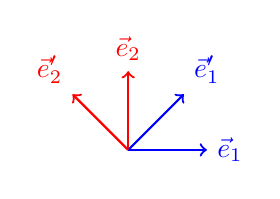
\begin{tikzpicture}[scale=0.5]
\coordinate (O) at (0,0);
\coordinate (X) at (2,0);
\coordinate (Y) at (0,2);
\coordinate (a) at (1.414,1.414);
\coordinate (b) at (-1.414,1.414);
\draw[->,thick,blue](O)--(X) node[pos=1,right] {$\vec{e}_1$};
\draw[->,thick,red](O)--(Y) node[pos=1,above] {$\vec{e}_2$};
\draw[->,thick,blue](O)--(a) node[pos=1,above right] {$\vec{e}'_1$};
\draw[->,thick,red](O)--(b) node[pos=1,above left] {$\vec{e}'_2$};
\end{tikzpicture}
\end{equation*}
\pp
$\Rightarrow (e_1',e_2') = (e_1,e_2)\begin{pmatrix}
\cos\theta&-\sin\theta\\\sin\theta&\cos\theta\\
\end{pmatrix}$
\pp
$\Rightarrow \begin{pmatrix} x\\y\\\end{pmatrix}= \begin{pmatrix}
\cos\theta&-\sin\theta\\\sin\theta&\cos\theta\\
\end{pmatrix}\begin{pmatrix} x'\\y'\\\end{pmatrix}.$
\pp
$\Rightarrow
\begin{pmatrix} x'\\y'\\\end{pmatrix}
= \begin{pmatrix}
\cos\theta&-\sin\theta\\\sin\theta&\cos\theta\\
\end{pmatrix}^{-1} \begin{pmatrix} x\\y\\\end{pmatrix}= \begin{pmatrix}
\cos\theta&\sin\theta\\-\sin\theta&\cos\theta\\
\end{pmatrix} \begin{pmatrix} x\\y\\\end{pmatrix}.$
\end{frame}








\subsection{线性方程组解集的结构}

\subsubsection{解空间}
\begin{frame}\frametitle{解空间}
\begin{example}
证明$V=\{(x_1,x_2,x_3)\in\bR^3\mid x_1+x_2+x_3=0\}$为$\bR^3$的子空间.求$V$的维数并找出其一组基.
\end{example}
\pp
\yang{通解: $X = t_1\begin{pmatrix} 1\\-1\\0\end{pmatrix} + t_2\begin{pmatrix} 1\\0\\-1\end{pmatrix}$.}
\pp
\begin{example}
证明 $W=\{(x_1,x_2,x_3)\in\bR^3\mid x_1+x_2+x_3=0,2x_1-x_2+x_3=3\}$不是$\bR^3$的子空间.
\end{example}
\pp
设$A\in \bF^{m\times n}$, $b\in \bF^m$为非零向量.\pp 则 \begin{enumerate}
\item $V:=\{X\in \bF^n\mid AX=0\}$为子空间;
\item $W:=\{X\in \bF^n\mid AX=b\}$不是子空间.
\end{enumerate}
接下来学习$V$和$W$更进一步地性质.
\end{frame}

%







\subsubsection{有(唯一)解的判定}
\begin{frame}\frametitle{有(唯一)解的判定}
\begin{theorem}
设$A\in \bF^{m\times n}$, $b\in \bF^m$.\pp 则
\begin{enumerate}
\item $AX=b$有解 $\Leftrightarrow$ $\rank(A)=\rank(A,b)$.\pp
\item $AX=b$有唯一解 $\Leftrightarrow$ $\rank(A)=\rank(A,b)=n$.
\end{enumerate}
\end{theorem}
\pp
\begin{example}
设$A\in \bF^{m\times n}$.\pp 则
\begin{enumerate}
\item $AX=0$一定有解;\pp
\item $AX=0$有非零解 $\Leftrightarrow$ $\rank(A)<n$ $\xLeftrightarrow{\text{若$A$为方阵}}$ $\det(A)=0$.
\end{enumerate}
\end{example}

\end{frame}





\subsubsection{齐次线性方程组的解空间}
\begin{frame}\frametitle{齐次线性方程组的解空间}
\pp
\begin{definition}[基础解系]
设$A\in \bF^{m\times n}$.\pp 称解空间\footnote{$V$也称为矩阵$A$的\blue{零空间}，记为\blue{$N(A)$}.}
\[V=\{X\in \bF^n\mid AX=0\}\]
的一组基为齐次线性方程组$AX=0$的一个\blue{基础解系}.
\end{definition}
\pp
\begin{theorem}[解空间大小]
\[\dim(V) = n-\rank(A).\]
\end{theorem}

\end{frame}









% ========== 2023年04月23号 第15次课 习题课 ==========


% ========== 2023年04月25号 第16次课 一般线性空间 ==========
%\frame{\titlepage}



\renewcommand{\mydate}{2025年04月17号\ 第十六次课}


\subsubsection{齐次线性方程组的解空间与线性映射的核*}
\begin{frame}\frametitle{齐次线性方程组的解空间与线性映射的核*}
\pp
给定矩阵$A\in\bF^{m\times n}$.\pp 通过$\mA(\vec{x}):=A\vec{x}$,我们可定义一个线性映射
\[\mA\colon \bF^n \rightarrow \bF^m.\]
\pp
\begin{proposition}
线性映射$\mA$的核正好为齐次线性方程组$AX=0$的解空间.\pp 即
\[\ker\mA = \{X\in \bF^n \mid AX=0\}.\]
\end{proposition}
\pp
此外,我们还有
\begin{proposition}
\begin{itemize}
\item 线性映射$\mA$的像由$A$的全体列向量生成;
\footnote{称$A$的列向量生成的子空间为$A$的\blue{列空间}.
类似地, 称$A$的行向量生成的子空间为$A$的\blue{行空间}.}
\pp
\item $\dim(\ker\mA) + \dim(\mathrm{im}\mA) = n$.
\end{itemize}
\end{proposition}
\end{frame}





\subsubsection{非齐次线性方程组的解空间}
\begin{frame}\frametitle{非齐次线性方程组的解空间}
如何描述非齐次线性方程组的解空间?
\pp
\[W:=\{X\in \bF^n\mid AX=b\}\]
$W$和$V$有什么联系?
\pp
基本事实:
\begin{itemize}
\item $\forall \alpha,\beta \in W$ $\Rightarrow$ $\alpha-\beta\in V$.\pp
\item $\forall \alpha\in W,\gamma\in V$ $\Rightarrow$ $\alpha+\gamma\in W$.
\end{itemize}
\pp
\begin{theorem}
若$W$非空,任取$\gamma_0\in W$,记 $\gamma_0+V:=\{\gamma_0+\alpha\mid \alpha \in V\}$.\pp 则
\[W=\gamma_0+V.\]
\end{theorem}
\pp
\yang{几何解释?}
\end{frame}






\subsection{一般线性空间的定义}



\subsubsection{一般线性空间引入}
\begin{frame}\frametitle{一般线性空间}
\pp
\blue{$n$维数组空间} = 赋予了加法和数乘运算的$n$维数组向量组成的集合.
\pp
\begin{equation*}
\xymatrix{
\text{加法,数乘} \ar[r] & \text{线性组合} \ar[r] & \text{线性相关(无关),等价} \ar[d]\\
& \text{秩,基,维数} \ar[dl] \ar[d] \ar[dr] &\text{极大无关组} \ar[l]\\
\text{坐标}&\text{过渡矩阵}&\text{扩充基}\\
}
\end{equation*}
\pp
\blue{问题:} 能否赋予其他集合``+''和``$\cdot$''，使得其满足类似的性质和结构?
\pp
\begin{example}
$\bF_n[x]:=\{a_0+a_1x+\cdots+a_nx^n \mid a_i\in \bF \text{ 对所有的 } i=0,1,\cdots,n\}$. \pp
\begin{itemize}
\item 加法 $(a_0+\cdots+a_nx^n)+(b_0+\cdots+b_nx^n):=(a_0+b_0)+\cdots+(a_n+b_n)x^n$;\pp
\item 数乘 $\lambda(a_0+\cdots+a_nx^n):=(\lambda a_0)+\cdots+(\lambda a_n)x^n$.
\end{itemize}
\pp
$\Rightarrow$ 多项式的线性相关,线性无关,极大无关组,秩,基.\\
e.g. $x^2+1$, $x^2$, $1$ 线性相关, $1,x,\cdots,x^n$为一组基.
\end{example}
\end{frame}





\begin{frame}\frametitle{一般线性空间}
\begin{example}
$\bF^{m\times n}$ 数域$\bF$上的全体$m\times n$矩阵. \pp
\begin{itemize}
\item 矩阵的加法; \pp
\item 矩阵的数乘. \pp
\end{itemize}
$\Rightarrow$ 矩阵的线性相关,线性无关,极大无关组,秩,基.\pp \\
e.g.
$\begin{pmatrix}1&0\\0&0\end{pmatrix}$,
$\begin{pmatrix}0&1\\0&0\end{pmatrix}$,
$\begin{pmatrix}0&0\\1&0\end{pmatrix}$,
$\begin{pmatrix}0&0\\0&1\end{pmatrix}$构成$\bF^{2\times2}$的一组基.
\end{example}
\pp
\begin{example}
$E_n:=\{a_1x_1+\cdots+a_nx_n=b\mid a_i,b\in \bF\}$.\pp
\begin{itemize}
\item 加法 $(a_1x_1+\cdots+a_nx_n=b)+(a_1'x_1+\cdots+a_n'x_n=b'):=\Big((a_1+a_1')x_1+\cdots+(a_n+a_n')x_n=(b+b')\Big)$;\pp
\item 数乘 $\lambda(a_1x_1+\cdots+a_nx_n=b) = (\lambda a_1x_1+\cdots+\lambda a_nx_n=\lambda b)$\pp
\end{itemize}
$\Rightarrow$ 线性方程组的线性相关,线性无关,极大无关组(等价的独立方程组),秩(独立方程的个数),基.
\end{example}
\end{frame}





\subsubsection{一般线性空间定义}
\begin{frame}\frametitle{一般线性空间定义}
设$V$为一个非空集. $\bF$为一个数域. 若$V$上存在两个运算\pp
\begin{enumerate}
\item \blue{加法}: 任意$V$中的有序对$(\alpha,\beta)$,存在唯一的$\gamma\in V$与之对应.记为$\alpha+\beta$. 即, $V\times V \rightarrow V \quad (\alpha,\beta)\mapsto \alpha+\beta$. \pp
\item \blue{数乘}: 任意$\lambda\in \bF$, 任意$\alpha\in V$, 存在唯一的$\gamma\in V$与之对应.记为$\lambda\alpha$. 即, $\bF\times V\rightarrow V \quad (\lambda,\alpha)\mapsto \lambda \alpha$.
\pp
\end{enumerate}
满足如下规律(\blue{八大公理}): \pp
\begin{enumerate}
\item A1): $\alpha+\beta=\beta+\alpha$,\quad $(\forall\alpha,\beta)$; \pp
\item A2): $\alpha+(\beta+\gamma)=(\alpha+\beta)+\gamma$,\quad $(\forall\alpha,\beta,\gamma)$; \pp
\item A3): $\exists\theta\in V\quad s.t. \quad \alpha+\theta=\alpha=\theta+\alpha$,\quad $(\forall\alpha)$, 这个$\theta$也常记为$0$; \pp
\item A4): $\forall \alpha \quad \exists \beta\in V \quad s.t. \quad \alpha+(\beta)=\theta=(\beta)+\alpha$, 称$\beta$为$\alpha$的负元记为$-\alpha$,定义减法为: $\gamma-\alpha=\gamma+(-\alpha)$; \pp
\item D1): $(\lambda+\mu)\alpha=\lambda \alpha + \mu \alpha$,\quad $(\forall \lambda,\mu,\alpha)$; \pp
\item D2): $\lambda (\alpha+\beta) =\lambda \alpha + \lambda \beta$,\quad $(\forall\lambda,\alpha,\beta)$; \pp
\item M1): $\lambda(\mu \alpha)=(\lambda \mu)\alpha$,\quad $(\forall\lambda,\mu,\alpha)$; \pp
\item M2): $1\alpha = \alpha$,\quad $(\forall\alpha)$;
\end{enumerate}\pp
则称$V$为$\bF$上的\blue{线性空间}. \pp $V$中的元素称为\blue{向量}.  \pp
\end{frame}





\subsubsection{公理体系的完备性}
\begin{frame}\frametitle{公理体系的完备性}
八条公理保证了抽象的线性空间有好的性质和结构.\pp
\begin{example}
设$\alpha_1,\cdots,\alpha_m$为$\bF$上的线性空间$V$上的一组向量.\pp 若存在一组不全为零的常数$\lambda_1,\cdots,\lambda_m$使得
\[\lambda_1\alpha_1 + \lambda_2\alpha_2 + \cdots \lambda_m\alpha_m =\theta,\]
\pp
则存在 $i$ 使得
\[\alpha_i = -\frac{\lambda_1}{\lambda_i}\alpha_1 -\frac{\lambda_{i-1}}{\lambda_{i}}\alpha_{i-1} -\frac{\lambda_{i+1}}{\lambda_{i}}\alpha_{i+1} -\frac{\lambda_m}{\lambda_i}\alpha_m.\]
\end{example}
\end{frame}





\subsubsection{线性空间的一种判定方法}
\begin{frame}\frametitle{线性空间的一种判定方法}
\begin{proposition}
设集合$V$上带有两个运算
\[\oplus\colon V\times V\rightarrow V、\qquad \text{和} \qquad \odot \colon \bF\times V\rightarrow V.\]
\pp
若存在正整数$n$和一个双射
\[\varphi\colon V\rightarrow \bF^n\]
满足以下两条
\pp
\begin{enumerate}
\item $\varphi(a\oplus b) = \varphi(a) + \varphi(b)$ \quad $(\forall a,b\in V)$; \pp
\item $\varphi(\lambda \odot a) = \lambda \varphi(a)$ \quad $(\forall a\in V),\forall\lambda\in \bF$,
\end{enumerate}
\pp
则$V$为$\bF$上的线性空间.
\end{proposition}
\begin{example}
$\bF=\bR$, $V:=\bR^+:=\{r\in\bR\mid r > 0\}$, $r_1\oplus r_2:=r_1r_2$, $\lambda\circ \alpha:=\alpha^\lambda$.
\end{example}
\end{frame}









% ========== 2023年04月27号 第17次课 一般线性空间 ==========
%\frame{\titlepage}





\subsubsection{常见的线性空间}
\begin{frame}\frametitle{常见的线性空间}

\begin{proposition}
\begin{enumerate}
\item 零向量$\theta$唯一;\pp
\item 负向量唯一;\pp
\item $0\alpha =\theta$, $(-1)\alpha=-\alpha$, $\lambda\theta=\theta$;\pp
\item $\lambda\alpha = \theta$ $\Rightarrow$ $\lambda=0$ 或 $\alpha=\theta$.
\end{enumerate}
\end{proposition}

\begin{example}
\begin{enumerate}
\item $\bF^n$;\pp
\item $E_n$: $n$元线性方程全体;\pp
\item $\bF_n[x]$: $\bF$上次数不超过$n$的多项式全体;\pp
\item $\bF^{m\times n}$;\pp
\item $\bF=\bR$, $V=\bC$;\pp
\item $\bF=\bR$, $V:=\bR^+:=\{r\in\bR\mid r > 0\}$, $r_1\oplus r_2:=r_1r_2$, $\lambda\circ \alpha:=\alpha^\lambda$.\pp
\item $C_n:=\{a_0+a_1\cos\theta+b_1\sin\theta+\cdots+a_n\cos(n\theta)+b_n\sin(n\theta)\mid a_i,b_i\in \bF\}$;\pp
\item $C[a,b]$ 区间$[a,b]$上的连续函数全体;
\end{enumerate}
\end{example}
\end{frame}


\renewcommand{\mydate}{2025年04月22号\ 第十七次课}


\subsubsection{线性空间反例}
\begin{frame}\frametitle{线性空间反例}

\begin{example}[反例]
\begin{enumerate}
\item $\bF=\bR$, $V=\bR^+$, 通常$+\times$ \pp
\item $\bF=\bR$, $v_0\in \bF^n$, $V:=\{v\in \bF^n\mid  v\nparallel v_0\}$, 通常$+\times$;\pp
\item $\bF=\bC$, $V=\bR_n[x]$ 通常$+\times$; \pp
\end{enumerate}
\end{example}

注: 一般线性空间没有长度和夹角等几何概念.
\end{frame}





\subsubsection{子空间}
\begin{frame}\frametitle{子空间}
\begin{definition}
设$V$为$\bF$-线性空间, $W$为$V$的非空子集, 若
\begin{enumerate}
\item 任取$\alpha,\beta\in W$,都有$\alpha+\beta\in W$;
\item 任取$\alpha\in W$以及$\lambda\in \bF$,都有$\lambda\alpha\in W$.
\end{enumerate}
则称$W$为$V$的\blue{子空间}.
\end{definition}
\pp
\begin{example}
\begin{enumerate}
\item 平凡子空间: $W=\{0\}$ 或者 $W=V$.\pp
\item 生成子空间: 任意子集 $S\subseteq V$, \\
$\langle S\rangle:=\{\lambda_1\alpha_1+\cdots+\lambda_n\alpha_n\mid \lambda_1,\cdots,\lambda_n\in \bF,\alpha_1,\cdots,\alpha_n\in S\}$.\pp
\item $\bF_n[x],C_n \subset C[a,b]$\pp
\item $W=\{P\in \bF_n[x]\mid P(x)=P(-x)\}\subset \bF_n[x]$;\pp
\item 任意 $A\in \bF^{n\times n}$, $W:=\{X\in \bF^{n\times n}\mid AX=0\}\subseteq \bF^{n\times n}$.
\end{enumerate}
\end{example}
\end{frame}

%









\subsection{一般线性空间的理论}





\subsubsection{数组向量空间上的概念以及性质推广到一般线性空间}
\begin{frame}\frametitle{数组向量空间上的概念以及性质推广到一般线性空间}
前面关于数组空间的绝大部分结论都可以平行的推广到一般线性空间上(只需要,证明过程中只涉及加法和数乘).
\pp
\begin{equation*}
\xymatrix{
\text{加法,数乘} \ar[r] & \text{线性组合} \ar[r] & \text{线性相关(无关),等价} \ar[d]\\
& \text{秩,基,维数} \ar[dl] \ar[d] \ar[dr] &\text{极大无关组} \ar[l]\\
\text{坐标}&\text{过渡矩阵}&\text{扩充基}\\
}
\end{equation*}

\end{frame}





\subsubsection{线性相关性}
\begin{frame}\frametitle{线性相关性}
\begin{theorem}[线性相关等价刻画] \small
给定向量空间$v$上的一组向量 $\alpha_1$, $\alpha_2$, $\cdots$, $\alpha_m$. 则以下几条相互等价:\pp
\begin{enumerate}
\item $\alpha_1$, $\alpha_2$, $\cdots$, $\alpha_m$ 线性相关. 即,存在不全为零的$\lambda_1,\lambda_2,\cdots,\lambda_{m}$使得\\ $\qquad\Sigma_{i=1}^m \lambda_i\alpha_i=\theta$. \pp
\item 存在$i\in\{1,\cdots,m\}$以及$\lambda_1\cdots\lambda_{i-1},\lambda_{i+1},\cdots,\lambda_m\in \bF$ 使得\\
$\qquad\alpha_i = \Sigma_{j\neq i} \lambda_j \alpha_j$.\pp
\item 存在$i\in\{1,\cdots,m\}$ 使得\\
$\qquad\alpha_i \in \langle \alpha_1,\cdots,\alpha_{i-1},\alpha_{i+1},\cdots,\alpha_m\rangle$.\pp
\item 存在$i\in\{1,\cdots,m\}$使得\\
$\qquad\langle \alpha_1,\alpha_{2},\cdots,\alpha_m\rangle = \langle \alpha_1,\cdots,\alpha_{i-1},\alpha_{i+1},\cdots,\alpha_m\rangle$.
\end{enumerate}
\end{theorem}
\pp
\yang{注: 这时候没有与``$AX=0$有非零解''的等价形式.}

\begin{theorem}
若$S_1\subseteq S\subseteq V$,\pp 则
\begin{enumerate}
\item $S_1$线性相关 $\Rightarrow$ $S$线性相关;\pp
\item $S$线性无关 $\Rightarrow$ $S_1$线性无关;
\end{enumerate}
\end{theorem}

\end{frame}





\subsubsection{极大无关组}
\begin{frame}\frametitle{极大无关组}

\pp
\begin{definition}[极大线性无关组]
设$\alpha_1$, $\alpha_2$, $\cdots$, $\alpha_m$为向量空间$v$上的一组向量.\pp 若
\begin{itemize}
\item 子向量组$\alpha_{i_1}$, $\alpha_{i_2}$, $\cdots$, $\alpha_{i_r}$线性无关,且\pp
\item 任加另一个向量$\alpha_{i_{r+1}}$后,向量组$\alpha_{i_1}$, $\alpha_{i_2}$, $\cdots$, $\alpha_{i_{r+1}}$线性相关,
\end{itemize}
\pp
则称$\alpha_{i_1}$, $\alpha_{i_2}$, $\cdots$, $\alpha_{i_r}$为$\alpha_1$, $\alpha_2$, $\cdots$, $\alpha_m$的\blue{极大无关组}.
\end{definition}
\pp
\begin{theorem}
若$S_1\subseteq S\subseteq V$, 则以下几条等价:\pp
\begin{enumerate}
\item $S_1$为$S$的极大无关组;\pp
\item $\left\{\begin{array}{l}
\text{$S_1$线性无关},且\\
\text{$S$可由$S_1$线性表示}\\
\end{array}\right.$\pp
\item $\left\{\begin{array}{l}
\text{$S_1$线性无关},且\\
\text{$S$与$S_1$等价}\\
\end{array}\right.$\pp
\item $\left\{\begin{array}{l}
\text{$S_1$线性无关},且\\
\langle S\rangle=\langle S_1\rangle\\
\end{array}\right.$
\end{enumerate}
\end{theorem}
\end{frame}





\subsubsection{向量组的等价与秩}
\begin{frame}\frametitle{向量组的等价与秩}
\begin{definition}[向量组等价]
两个向量组称为\blue{等价},若它们可以相互线性表示.
\end{definition}
\pp
\begin{theorem}
两个等价线性无关的向量组个数相同.
\end{theorem}
\pp
\begin{definition}[秩]
一个向量组的\blue{秩}定义为其某个极大无关组中向量的个数.
\end{definition}
\pp
\begin{theorem}
设$S,T\subseteq V$.\pp 则
\begin{enumerate}
\item $S$线性无关 $\Leftrightarrow$ $\rank(S)=\#S$;\pp
\item $S$线性相关 $\Leftrightarrow$ $\rank(S)<\#S$;\pp
\item $T$可由$S$线性表示 $\Rightarrow$ $\rank(T)\leq
\rank(S)$;\pp
\item $S\sim T$ $\xLeftrightarrow{T\text{可由}S\text{线性表示}}$ $\rank(T) = \rank(S)$;\pp
\item $T$可由$S$线性表示且$T$的线性无关 $\Rightarrow$ $\#T\leq \#S$.
\end{enumerate}
\end{theorem}
\end{frame}





\subsubsection{基、维数与坐标}
\begin{frame}\frametitle{基、维数与坐标}
\begin{definition}
\begin{enumerate}
\item 设$V$为线性空间.\pp 若$S\subseteq V$线性无关,且 $V=\langle S\rangle$,\pp 则称$S$为$V$的\blue{一组基}. \pp
\item 设$S$为一组基.\pp 若$S$为有限集,则称$V$为\blue{有限维空间},\pp 否则称之为\blue{无限维线性空间}.\pp 称$S$的个数为$V$的\blue{维数},\pp 记作 \blue{$\dim_\bF V$}.\pp
\item 若$S=\{\alpha_1,\cdots,\alpha_n\}$为$V$的一组基,则对任意$\alpha\in V$,存在唯一的$n$维数组向量 $(\lambda_1,\cdots,\lambda_n)\in \bF^n$使得
$\alpha = \sum\limits_{i=1}^n \lambda_i\alpha_i.$ \pp
称向量$(\lambda_1,\cdots,\lambda_n)$为$\alpha$在$S$下的\blue{坐标}.
\end{enumerate}
\end{definition}
\pp
\begin{theorem}
\begin{enumerate}
\item $n$维空间中的任意$n+1$个向量线性相关. \pp
\item $n$维空间中的任意$n$个线性无关的向量组为一组基.\pp
\item $n$维空间中的任意线性无关的向量组可扩充为一组基.
\end{enumerate}
\end{theorem}
\end{frame}






\begin{frame}\frametitle{例子}
\begin{example}
$\{1,\cos\theta,\sin\theta,\cos(2\theta),\sin(2\theta)\}$为$\{1,\cos\theta,\sin\theta,\cos^2(x),\sin^2(x),\cos(2\theta),\sin(2\theta)\}$的一个极大无关组.
\end{example}
\pp
\begin{example}
设 $T\subseteq S\subseteq V$. 则
\[\rank(S)-\rank(T) \leq \#S- \#T.\]
\end{example}
\pp
\yang{证明: 设$S_1$为$S$的极大无关组,则$S_1\cap T$线性无关.\pp 因此
\[\rank(T) \geq \rank(S_1\cap T) =\#S_1+\#T-\#(S_1\cup T)\geq \rank(S)+\#T-\#S.\]}

\pp
\begin{example}
\begin{enumerate}
\item $\dim_\bR \bC = 2$; \pp $\dim_\bF \bF[x] = \infty$; \pp $\dim_\bF \bF^{m\times n}=mn$. \pp
\item 记 $W=\{f(x)\in\bF[x]\mid\deg f(x)\leq n,f(2)=0\}$. 则$W$是$\bF[x]$的子空间.则$W$有一组基\underline{\qquad\qquad\qquad}.
\end{enumerate}
\end{example}
\end{frame}





\begin{frame}\frametitle{例子}
\begin{example}
求线性空间$\bF_{n-1}[x]$从基$\{1,x,\cdots,x^{n-1}\}$到基$\{1,x+1,\cdots,(x+1)^{n-1}\}$的过渡矩阵.
\end{example}
\pp
\begin{example}矩阵
$\begin{pmatrix}1&0\\0&0\\\end{pmatrix}$,
$\begin{pmatrix}1&2\\0&0\\\end{pmatrix}$,
$\begin{pmatrix}1&2\\3&0\\\end{pmatrix}$,
$\begin{pmatrix}1&2\\3&4\\\end{pmatrix}$构成线性空间$\bF^{2\times2}$的一组基.\pp 这组基到$\bF^{2\times2}$的自然基$E_{11},E_{12},E_{21},E_{22}$的过渡矩阵为\underline{\qquad\qquad\qquad}.
\end{example}
\end{frame}



\subsection{子空间*}




% ========== 2023年05月04号 第18次课 子空间运算与线性映射 ==========
%\frame{\titlepage}





\subsubsection{子空间的运算*}
\begin{frame}\frametitle{子空间的运算*}
\yang{如何从已有的子空间构造新的子空间?}
\pp
\yang{子空间的交还是子空间.}
\pp
\begin{theorem}
设 $W_i$($i\in I$)为$V$的子空间,则$\cap_{i\in I}W_i$也为$V$的子空间.\pp 特别地,设$W_1$, $W_2$为$V$的子空间,则$W_1\cap W_2$也为$V$的子空间.
\end{theorem}

\yang{并集呢?}
\pp
\yang{几何解释?}
\pp
\yang{包含并集的最小子空间?}
\pp
\begin{theorem}
设$W_1$, $W_2$为$V$的子空间,则$W_1$与$W_2$的和
\[W_1+W_2:=\{\alpha_1+\alpha_2 \mid \alpha_1\in W_1,\alpha_2\in W_2\}\]
构成$V$的子空间,并且是包含 $W_1\cup W_2$的最小子空间.
\end{theorem}

\end{frame}





\subsubsection{维数公式}
\begin{frame}\frametitle{维数公式}
\begin{lemma}
$\langle\alpha_1,\cdots,\alpha_r\rangle + \langle\beta_1,\cdots,\beta_s\rangle = \langle\alpha_1,\cdots,\alpha_r,\beta_1,\cdots,\beta_s\rangle$.
\end{lemma}
\pp
\begin{theorem}[维数公式]设$W_1$, $W_2$为$V$的子空间,则
\[\dim(W_1+W_2) = \dim(W_1) + \dim(W_2) - \dim(W_1\cap W_2).\]
\end{theorem}
\pp
\yang{证明思路:扩充 $W_1\cap W_2$ 的一组基.\\ \pp
记 $r=\dim W_1$, $s=\dim W_2$ 以及 $t=\dim W_1\cap W_2$. \pp 将$W_1\cap W_2$一组基$\alpha_1,\cdots,\alpha_t$扩充为
\[\left\{{
\text{$W_1$的一组基: } \alpha_1,\cdots,\alpha_t,\beta_1,\cdots,\beta_{r-t}
\atop
\text{$W_2$的一组基: } \alpha_1,\cdots,\alpha_t,\gamma_1,\cdots,\gamma_{s-t}
}\right.\]
\pp
则 $W_1+W_2 = \langle\alpha_1,\cdots,\alpha_t,\beta_1,\cdots,\beta_{r-t},\gamma_1,\cdots,\gamma_{s-t}\rangle$. \pp 下面仅需证明这$r+s-t$个向量线性无关.
}
\end{frame}






\begin{frame}\frametitle{维数公式}

\begin{corollary}
设$W_1$, $W_2$为$V$的子空间.\pp 则
\begin{enumerate}
\item $\dim(W_1+W_2) \leq \dim(W_1) + \dim(W_2)$;\pp
\item $\dim(W_1+W_2) = \dim(W_1) + \dim(W_2)\Leftrightarrow W_1\cap W_2 = \{0\}$;\pp
\item $\dim(W_1\cap W_2) \geq \dim(W_1) + \dim(W_2) - \dim(V)$.\pp 特别地,若 $\dim(W_1) + \dim(W_2) > \dim(V)$,则$W_1\cap W_2\neq\{0\}$.
\end{enumerate}
\end{corollary}
\end{frame}




\subsubsection{直和}
\begin{frame}\frametitle{直和}

\begin{definition}[直和]
设$W_1$, $W_2$为$V$的子空间.\pp 若任意$\alpha\in W_1+W_2$可\blue{唯一地}写成
\[\alpha = \alpha_1 + \alpha_2 \quad (\alpha_1\in W_1\ \&\ \alpha_2\in W_2),\]
则称 $W_1+W_2$为\blue{直和},记为$W_1\oplus W_2$.\pp 若$V=W_1\oplus W_2$,则称$W_1$为$W_2$的\blue{补空间}.
\end{definition}
\pp
注:补空间不唯一(例子). 如何构造补空间?扩充基!
\pp
\begin{theorem}
设$W_1$, $W_2$为$V$的子空间.则以下几条等价:\pp
\begin{enumerate}
\item $W_1+W_2$为直和;\pp
\item $W_1\cap W_2=\{0\}$;\pp
\item $\dim(W_1+W_2) = \dim(W_1) + \dim(W_2)$;\pp
\item 任取$W_1$的一组基$\alpha_1,\cdots,\alpha_r$和$W_2$的一组基$\beta_1,\cdots,\beta_s$,则$\alpha_1,\cdots,\alpha_r,\beta_1,\cdots,\beta_s$构成$W_1+W_2$的一组基.
\end{enumerate}
\end{theorem}
\end{frame}






\begin{frame}\frametitle{直和例子}
\begin{example}
\begin{center}
$\bF^{n\times n}$ = \{对称矩阵\} $\oplus$ \{反对称矩阵\}.
\end{center}
\end{example}
\pp
\begin{example}令 $W_1=\{(x_1,\cdots,x_n)\in \bF^n\mid x_1+\cdots+x_n=0\}$ 和 $W_2=\{(x_1,\cdots,x_n)\in \bF^n\mid x_1=x_2=\cdots=x_n\}$,则
\[\bF^{n} = W_1 \oplus W_2.\]
\end{example}
\pp
\begin{example}
\begin{center}
\{函数\} = \{奇函数\} $\oplus$ \{偶函数\}.
\end{center}
\end{example}
\end{frame}

\renewcommand{\mydate}{2025年04月24号\ 第十八次课}

%\setcounter{framenumber}{30}
\makeatletter
\ifodd\value{page}
\else
\begin{frame}[plain]
\end{frame}
\fi
\makeatother


\section{线性映射}


\title{第七章 \quad 线性映射}
\author{}
\date{}

\frame{\titlepage}

\subsection{线性映射}


\subsubsection{数组向量空间之间的线性变换与矩阵}
\begin{frame}\frametitle{数组向量空间之间的线性变换与矩阵}
给定一个数组向量空间之间的映射$\sA\colon \bF^n\rightarrow \bF^m$.
\pp
若$\sA$满足
\begin{equation}\label{equ:linearoperator}\tag{$*$}
\begin{split}
\blue{\text{(保持加法)\quad }} &\sA(\vec{a} + \vec{b}) = \sA(\vec{a}) + \sA(\vec{b});\\
\pp
\blue{\text{(保持数乘)\quad }} &\sA(\lambda\vec{a}) = \lambda\sA(\vec{a})
\end{split}
\end{equation}
\pp
则$\sA$称为从$\bF^n$到$\bF^m$的一个\blue{线性映射}.

\pp
\bigskip
我们有如下一一对应:
\begin{center}
\fbox{
从$\bF^n$到$\bF^m$的全体线性映射 \qquad $\xleftrightarrow[\sA(\vec{x})=A\vec{x}]{\quad 1:1\quad }$ \quad $\bF^{m\times n}$ }
\end{center}
\end{frame}






\begin{frame}\frametitle{例子}

\begin{example}[伸缩变换]
$\begin{pmatrix} x\\y\\\end{pmatrix}\mapsto \begin{pmatrix} k_1x\\k_2y\\\end{pmatrix} = \begin{pmatrix} k_1&\\&k_2\\\end{pmatrix}\begin{pmatrix} x\\y\\\end{pmatrix}$.
\end{example}
\pp
\begin{example}[旋转变换]
$\begin{pmatrix} x\\y\\\end{pmatrix}\mapsto \begin{pmatrix} x\cos\theta-y\sin\theta\\x\sin\theta+y\cos\theta\\\end{pmatrix} = \begin{pmatrix} \cos\theta&-\sin\theta\\\sin\theta&\cos\theta\\\end{pmatrix}\begin{pmatrix} x\\y\\\end{pmatrix}$.
\end{example}
\pp
\begin{example}
\begin{itemize}
\item[] $\bullet$ $\begin{pmatrix}1&\\&1\end{pmatrix}$ $\leftrightarrow$ \blue{恒等变换};
\pp
\qquad $\bullet$ $\begin{pmatrix}0&\\&0\end{pmatrix}$ $\leftrightarrow$ \blue{零变换};
\pp
\item[] $\bullet$  $\begin{pmatrix}\lambda&\\&\mu\end{pmatrix}$ $\leftrightarrow$ \blue{伸缩变换};
\pp
\qquad $\bullet$  $\begin{pmatrix}\cos\theta&-\sin\theta\\\sin\theta&\cos\theta\end{pmatrix}$ $\leftrightarrow$ \blue{旋转变换};
\pp
\item[] $\bullet$  $\begin{pmatrix}1&0\\0&-1\end{pmatrix}$ $\leftrightarrow$ \blue{反射变换};
\pp
\qquad $\bullet$  $\begin{pmatrix}1&\\&0\end{pmatrix}$ $\leftrightarrow$ \blue{投射变换};
\end{itemize}
\end{example}
\end{frame}



% ========== 2023年05月09号 第19次课 线性映射在基下的矩阵 ==========
%\frame{\titlepage}





\subsubsection{一般线性空间之间的线性变换}
\begin{frame}\frametitle{一般线性空间之间的线性变换}

接下来将线性映射推广到一般的线性空间上.

\begin{definition}[线性映射,线性变换和同构]
设$V$和$W$为两个$\bF$-线性空间.\gray{(注意:这里$V$和$W$不再要求是数组向量空间,而只是一般的线性空间.)}

\begin{enumerate}
\item 若映射$\sA\colon V\rightarrow W$满足
\begin{itemize}
\item  $\sA(P_1 + P_2) = \sA( P_1) + \sA(P_2)$;
\item  $\sA(\lambda P_1) = \lambda\sA( P_1)$.
\end{itemize}
则称$\sA$为从$V$到$W$的\blue{线性映射}.
\item 若$V=W$,则称线性映射$\sA$为$V$上的一个\blue{线性变换}.
\item 若线性映射$\sA$为双射,则称$\sA$为线性空间$V$到$W$的一个\blue{同构映射}. 若两个线性空间之间存在同构映射,则称它们互相\blue{同构}.
\end{enumerate}
\end{definition}
\pp
\begin{proposition}[同构基本性质]
\begin{itemize}
\item 同构映射的逆映射也是同构映射.
\pp
\item 同构为等价关系.
\pp
\item (同一域上的)有限维线性空间同构当且仅当它们维数相同.
\end{itemize}
\end{proposition}

\end{frame}






\begin{frame}\frametitle{例子}
\pp
\begin{example}
\begin{enumerate}
\item \blue{单位变换(恒等变换)}: $\varepsilon\colon V\rightarrow V$, $x\mapsto x$;
\pp
\item \blue{零映射}: $\varepsilon\colon V\rightarrow W$, $x\mapsto 0$;
\pp
\item \blue{微分变换}:
\[\sA\colon \bF_n[x] \rightarrow \bF_n[x],\quad p(x)\mapsto \frac{\mathrm{d}}{\mathrm{d}x}p(x).\]
\pp
\item \blue{积分变换}:
\[\sA\colon C[a,b]\rightarrow C[a,b],\quad f\mapsto \int_{a}^{b}K(x,t)f(t)\mathrm{d}t\]
其中 $K(x,t)$为$[a,b]\times[a,b]$上的实值连续函数.
\pp
\item \blue{线性化变换}: 记$V$为$[a,b]$上的函数集合. \[\sA:V\rightarrow V,\quad f\mapsto (1-x)f(a)+xf(b).\]
\pp
\item \blue{矩阵对应的线性映射}: $A\in \bF^{m\times n}$. \[\sA\colon \bF^n\rightarrow \bF^m,\quad x\mapsto Ax \text{(列向量)}.\]
\end{enumerate}
\end{example}
\end{frame}






\begin{frame}\frametitle{例子与反例}
\begin{example}
\begin{enumerate}\setcounter{enumi}{6}
\item \blue{投影映射}: $\sA\colon \bF^n\rightarrow \bF^r$, $(x_1,\cdots,x_n)\mapsto (x_1,\cdots,x_r)$;
\pp
\item \blue{嵌入映射}: $\sA\colon \bF^r\rightarrow \bF^n$, $(x_1,\cdots,x_r)\mapsto (x_1,\cdots,x_r,0,\cdots,0)$;
\pp
\item $\sA\colon \bF^n\rightarrow \bF^n$, $(x_1,x_2,\cdots,x_n)\mapsto (x_n,x_{n-1},\cdots,x_1)$;
\pp
\item 设$A\in \bF^{p\times m}$以及$B\in \bF^{n\times q}$为固定矩阵,
\[\sA\colon \bF^{m\times n}\rightarrow \bF^{p\times q},\quad X\mapsto AXB.\]
\pp
\item 设$V$为$\bF$上的线性空间, $\alpha_1,\cdots,\alpha_n$为 $V$中的任意 $n$个向量.
\[\sA\colon \bF^n \rightarrow V,\quad (x_1,\cdots,x_n) \mapsto x_1\alpha_1+\cdots+x_n\alpha_n.\]
\end{enumerate}
\end{example}
\pp

\begin{example}[反例]
\begin{enumerate}
\item $\sA\colon \bC^3 \rightarrow \bC^3$,  $(x,y,z)\mapsto (x^2,xy,z^2)$ 不是$\bC$-线性的.
\pp
\item $\sA\colon \bC \rightarrow \bC$, $z\mapsto \overline{z}$ 是$\bR$-线性的但不是$\bC$-线性的.
\end{enumerate}
\end{example}
\end{frame}





\subsubsection{线性变换基本性质}
\begin{frame}\frametitle{线性变换基本性质}

\begin{proposition}[线性映射的基本性质]
设$\sA$为从$\bF$-线性空间$V$到$\bF$-线性空间$W$的线性映射.
\pp
则
\begin{enumerate}
\item $\sA(0)=0$;
\pp
\item $\sA(-\alpha) = -\sA(\alpha)$, ($\forall \alpha\in V$);
\pp
\item 设$\alpha_1,\cdots,\alpha_n$为$V$的一组基. 若$\alpha = \lambda_1\alpha_1 + \cdots + \lambda_n\alpha_n$,则
\[\sA(\alpha) = \lambda_1\sA(\alpha_1) + \cdots + \lambda_n\sA(\alpha_n).\]
\pp
\yang{即,线性映射$\sA$由$\sA(\alpha_1),\cdots,\sA(\alpha_n)$这$n$个向量唯一确定.}
\pp
\item 若$\beta_1,\cdots,\beta_m$线性相关,则$\sA{\beta_1},\cdots,\sA{\beta_m}$也线性相关.
\pp
\item 若$\sA{\beta_1},\cdots,\sA{\beta_m}$线性无关,则$\beta_1,\cdots,\beta_m$也线性无关.
\end{enumerate}
\end{proposition}
\end{frame}





\subsection{线性映射与矩阵的对应}



\subsubsection{线性映射的矩阵*}
\begin{frame}\frametitle{线性映射的矩阵*}
设$\sA$为从$n$维$\bF$-向量空间$V$到$m$维$\bF$-向量空间的一个线性变换.分别取定$V$和$W$的一组基$\alpha_1,\cdots,\alpha_n$和$\beta_1,\cdots,\beta_m$.
\pp
对任意$j=1,2,\cdots,n$, 设$\sA(\alpha_j)\in W$ 在基$\beta_1,\cdots,\beta_m$下的坐标为$(a_{1j},\cdots,a_{mj})^T$,
\pp
即
\[\sA(\alpha_j) = a_{1j}\beta_1 + \cdots + a_{mj}\beta_m.\]
\pp
则这一式子可改写为
\[\blue{\sA(\alpha_1,\cdots,\alpha_n)  := \Big(\sA(\alpha_1),\cdots,\sA(\alpha_n)\Big) = (\beta_1,\cdots,\beta_m)A},\]
其中 $A:=(a_{ij})_{m\times n}\in F^{m\times n}$.
\pp
称 $A$ 为\blue{线性映射 $\sA$ 在基 $\alpha_1,\cdots,\alpha_n$和$\beta_1,\cdots,\beta_m$下的矩阵}.
\pp
\begin{example}
设$A \in\bF^{m\times n}$. 定义从$\bF^n$到$\bF^m$的线性变换
\[\sA(X) = AX.\]
则$\sA$在自然基下的矩阵为$A$.
\end{example}
\pp
\yang{证: 记$e_1,\cdots,e_n$为$\bF^n$的自然基, $e'_1,\cdots,e'_m$为$\bF^m$的自然基.则
$\sA(e_1,\cdots,e_n):=(\sA e_1,\cdots,\sA e_n)=(A e_1,\cdots,A e_n)=A(e_1,\cdots,e_n)=AI_n=A=I_mA=(e'_1,\cdots,e'_m)A$.}
\end{frame}





\begin{frame}\frametitle{线性映射的矩阵*}
\begin{example}[从矩阵出发构造线性映射]
分别取定$\bF$-线性空间$V$和$W$的一组基$\alpha_1,\cdots,\alpha_n$和$\beta_1,\cdots,\beta_m$.
\pp
对于给定矩阵$B=(b_{ij})_{m\times n}\in \bF^{m\times n}$,如下给出一个从 $V$到 $W$的映射$\sB$.
\pp
对任意的$\lambda_1\alpha_1+\cdots+\lambda_n\alpha_n\in V$, 定义\footnote{这一定义也可改写为$\sB\left((\alpha_1,\cdots,\alpha_n)\begin{pmatrix}\lambda_1\\\vdots\\\lambda_n\\\end{pmatrix}\right) = (\beta_1,\cdots,\beta_n)B\begin{pmatrix}\lambda_1\\\vdots\\\lambda_n\\\end{pmatrix}$.}
\[\sB\left(\sum_{j=1}^n\lambda_j\alpha_j\right) := \sum_{i=1}^{m} \left(\sum_{j=1}^{n} b_{ij}\lambda_j\right) \beta_i.\]
\pp
则 $\sB$为从 $V$到 $W$的一个线性映射,且其在基$\alpha_1,\cdots,\alpha_n$和$\beta_1,\cdots,\beta_m$下的矩阵正好为$B$.
\end{example}
\pp
从而,我们得到如下一一对应:
\begin{center}
\fbox{
$\left\{\text{从$V$到$W$的}\atop \text{全体线性映射}\right\}$ \quad $\xleftrightarrow[1:1 \atop \sA(\alpha_1,\cdots,\alpha_n) = (\beta_1,\cdots,\beta_n)A]{\text{基} \alpha_1,\cdots,\alpha_n \atop \text{基} \beta_1,\cdots,\beta_m }$ \quad $\bF^{m\times n}$ }
\end{center}
\end{frame}





\subsubsection{线性映射的坐标表示*}
\begin{frame}\frametitle{线性映射的坐标表示*}
\begin{theorem} 设 $A$ 为线性映射 $\sA\colon V\rightarrow W$ 在基 $\alpha_1,\cdots,\alpha_n$和$\beta_1,\cdots,\beta_m$下的矩阵. \pp
若$X$为向量$v\in V$在基$\alpha_1,\cdots,\alpha_n$下的坐标,以及$Y$为$\sA(v)$在基$\beta_1,\cdots,\beta_m$下的坐标, 则
\[Y=AX.\]
\end{theorem}
\pp
换言之,线性映射的作用可以通过对坐标左乘矩阵$A$实现.
\pp
即,下图交换
\begin{equation*}
\xymatrix@C=5cm@R=2cm{
V
\ar[r]^{\text{基 }\alpha_1,\cdots,\alpha_n}_{1:1} \ar[d]^-{\sA}_{v\mapsto \sA(v)}
\ar@{}[dr]|{\tiny \blue{\sA(\alpha_1,\cdots,\alpha_n) = (\beta_1,\cdots,\beta_n)A}}
& \bF^n
\ar[d]_-{A}^{X\mapsto AX}\\
W \ar[r]^{\text{基 }\beta_1,\cdots,\beta_n}_{1:1} & \bF^m \\
}
\end{equation*}
\pp
\yang{证明思路: $\sA(v)=\sA((\alpha_1,\cdots,\alpha_n)X) = \sA(\alpha_1,\cdots,\alpha_n)\cdot X=(\beta_1,\cdots,\beta_m)A \cdot X= (\beta_1,\cdots,\beta_m) \cdot AX$.}
\end{frame}



\renewcommand{\mydate}{2025年04月29号\ 第十九次课}


\subsubsection{线性代数的核心*}
\begin{frame}\frametitle{线性代数的核心*}

\begin{table}[]
\begin{tabular}{|cc|}
\cline{1-2}
\multicolumn{2}{|c|}{几何 $\xleftrightarrow[\text{基}]{\text{坐标系}}$ 代数} \\ \cline{1-2}
\multicolumn{1}{|c|}{线性空间} & 数组空间\\ \cline{1-2}
\multicolumn{1}{|c|}{向量}   & 坐标 \\ \cline{1-2}
\multicolumn{1}{|c|}{\qquad 线性映射\qquad \qquad } & 基下矩阵 \\ \cline{1-2}
\multicolumn{1}{|c|}{内积} & 矩阵 \\ \cline{1-2}
\multicolumn{1}{|c|}{二次型} & 矩阵 \\ \cline{1-2}
\multicolumn{1}{|c|}{张量} & 由数组成的高维阵列 \\ \cline{1-2}
\multicolumn{1}{|c|}{...} & ... \\ \cline{1-2}
\end{tabular}
\end{table}

\end{frame}




\subsection{线性变换与方阵的对应}




\subsubsection{线性变换的矩阵}
\begin{frame}\frametitle{线性变换的矩阵}
现在,我们考虑$W$等于$V$的情形.

\pp \bigskip
设$\sA$为$V$上的线性变换.固定$V$的一组基$\alpha_1,\cdots,\alpha_n$. 则存在矩阵$A:=(a_{ij})_{n\times n}$使得
\[\sA(\alpha_1,\cdots,\alpha_n) = (\alpha_1,\cdots,\alpha_n)A.\]
\pp
称矩阵$A$为\blue{线性变换$\sA$在基$(\alpha_1,\cdots,\alpha_n)$下的矩阵}.
\pp

\begin{example}
设$V=\bF^{2\times 2}$.记$A=\begin{pmatrix}1&2\\3&4\end{pmatrix}\in V$. 定义$V$上的线性变换$\sA$
\[\sA(M):=AM.\]
求$\sA$在$e_{11},e_{12},e_{21},e_{22}$下的矩阵.
\end{example}
\pp

\begin{center}
\fbox{
$\left\{\text{从$V$到$V$的}\atop \text{全体线性变换}\right\}$ \quad $\xleftrightarrow[1:1 \atop \sA(\alpha_1,\cdots,\alpha_n) = (\alpha_1,\cdots,\alpha_n)A]{\text{基} \alpha_1,\cdots,\alpha_n}$ \quad $\bF^{n\times n}$ }
\end{center}
\end{frame}





\subsubsection{线性变换的坐标表示}
\begin{frame}\frametitle{线性变换的坐标表示}
向量$x$和$\sA x$在同一组基下坐标之间的关系.
\pp
\begin{theorem}
设$\sA\colon V\rightarrow V$在基$\alpha_1,\cdots,\alpha_n$下的矩阵为$A$.
\pp
若向量$x\in V$在基$\alpha_1,\cdots,\alpha_n$下的坐标$X\in \bF^n$, 向量$\sA x$在基$\alpha_1,\cdots,\alpha_n$下的坐标为 $Y\in \bF^n$,
\pp
则
\[Y=AX.\]
\end{theorem}
\pp
\begin{equation*}
\xymatrix@C=5cm@R=2cm{
V
\ar[r]^{\text{基 }\alpha_1,\cdots,\alpha_n}_{1:1} \ar[d]_-{\sA}
\ar@{}[dr]|{\tiny \sA(\alpha_1,\cdots,\alpha_n) = (\alpha_1,\cdots,\alpha_n)A}
& \bF^n
\ar[d]^-{A}\\
V \ar[r]^{\text{基 }\alpha_1,\cdots,\alpha_n}_{1:1} & \bF^n \\
}
\end{equation*}
\end{frame}






\begin{frame}\frametitle{}

\begin{example}
记 $\alpha_1=\begin{pmatrix}2\\3\\5\end{pmatrix}$, $\alpha_2=\begin{pmatrix}0\\1\\2\end{pmatrix}$, $\alpha_3=\begin{pmatrix}1\\0\\0\end{pmatrix}$,
$\beta_1=\begin{pmatrix}1\\2\\0\end{pmatrix}$, $\beta_2=\begin{pmatrix}2\\4\\-1\end{pmatrix}$, $\beta_3=\begin{pmatrix}3\\0\\5\end{pmatrix}$.
\pp
设$\sA$为$\bF^3$上线性变换满足 $\sA(\alpha_i)=\beta_i$ ($i=1,2,3$).
\pp
求
\begin{enumerate}
\item $\sA$在$\alpha_1,\alpha_2,\alpha_3$下的矩阵;
\item $\sA$在自然基下的矩阵.
\end{enumerate}
\end{example}
\pp
\yang{解答:}
\begin{enumerate}
\item \yang{$A=(\alpha_1,\alpha_2,\alpha_3)^{-1}(\beta_1,\beta_2,\beta_3)=\begin{pmatrix}
4&9&-5\\-10&-23&15\\-7&-16&13\\\end{pmatrix}$;}
\item \yang{$B=(\beta_1,\beta_2,\beta_3)(\alpha_1,\alpha_2,\alpha_3)^{-1}=\begin{pmatrix}
3&-20&11\\0&-16&10\\5&-15&7\\\end{pmatrix}$.}
\end{enumerate}

\end{frame}









% ========== 2023年05月11号 第20次课 线性映射的矩阵与相抵关系,线性变换的矩阵与相似关系,对偶空间 ==========
%\frame{\titlepage}





\subsubsection{矩阵对应的线性变换}
\begin{frame}\frametitle{矩阵对应的线性变换}
设$\alpha_1,\cdots,\alpha_n$为$n$维$\bF$-线性空间$V$的一组基.
\begin{equation*}
\xymatrix@C=2cm@R=0cm{
\text{$V$上的线性变换}
\ar[r]^{\alpha_1,\cdots,\alpha_n}_{1:1}	& \bF^{n\times n} \\
\sA \ar@{|->}[r] & \text{ $\sA$在$\alpha_1,\cdots,\alpha_n$下的矩阵}\\
?? & B \ar@{|->}[l]\\
}
\end{equation*}
反之,给定$n$阶矩阵$B=(b_{ij})_{n\times n}$,我们可以如下定义一个映射(对于任意$\alpha=x_1\alpha_1+\cdots+x_n\alpha_n\in V$)
\[\sB(\alpha):=\sum_{i=1}^n\left(\sum_{j=1}^n b_{ij}x_j\right)\alpha_i = (\alpha_1,\cdots,\alpha_n)B\begin{pmatrix}x_1\\\vdots\\x_n\end{pmatrix}\]
\begin{proposition}
映射$\sB$为$V$上的线性变换,且其在$\alpha_1,\cdots,\alpha_n$下的矩阵为$B$.
\end{proposition}
\end{frame}





\subsubsection{线性映射的运算*}
\begin{frame}\frametitle{线性映射的运算*}
设$U$, $V$和$W$为有限维$\bF$-线性空间.
\pp
\begin{enumerate}
\item \blue{(加法)} 设$\sA$和$\sB$为从$V$到$W$的两线性映射. 对任意$v\in V$,定义
\[(\sA+\sB)(v):=\sA(v)+\sB(v);\]
\pp
\item \blue{(数乘)} 设$\sA$为从$V$到$W$的线性映射. 对于任意$v\in V$,定义
\[(\lambda\sA)(v):=\lambda\sA(v);\]
\pp
\item \blue{(合成)} 设$\sA$为从$V$到$W$的线性映射,$\sB$为从$U$到$V$的线性映射. 对于任意$u \in U$,定义
\[(\sA\circ\sB)(u):=\sA\left(\sB(u)\right).\]
\end{enumerate}
\pp
\begin{proposition}
\begin{enumerate}
\item 以上三者均为线性映射的运算.即, $\sA+\sB$, $\lambda\sA$和$\sA\circ\sB$仍为线性变换.
\pp
\item 若各自取定$U$, $V$和$W$的一组基, 设$\sA$,$\sB$在这些基下的矩阵分别为$A$,$B$, 则$\sA+\sB$, $\lambda\sA$和$\sA\circ\sB$在这些基下的矩阵分别为 $A+B$, $\lambda A$ 和 $AB$.
\pp
\item 从$V$到$W$上的全体线性映射组成的集合,记为 $\blue{\mathrm{Hom}(V,W)}$, 在线性映射的加法和数乘下构成$\bF$-线性空间.
\end{enumerate}
\end{proposition}
\end{frame}




\subsubsection{多项式在线性变换处取值}
\begin{frame}\frametitle{多项式在线性变换处取值}
设$\sA$和$\sB$为$\bF$-线性空间$V$上的线性变换.
\pp
记 $\blue{\sA^0}:=\mathrm{id}(:=\varepsilon)$.
\pp
对任意正整数$k$, 定义
\[\blue{\sA^k}:=\underbrace{\sA\circ\sA\circ\cdots\circ\sA}_{k\text{次}}.\]
\pp
对于$f(x)=a_0+a_1x+\cdots+a_nx^n\in \bF[x]$,定义
\[\blue{f(\sA)} := a_0\cdot\varepsilon + a_1\sA + \cdots a_n\sA^n.\]
\pp
\begin{example}
若$\sA$在$V$的某组基$e_1,\cdots,e_n$下的矩阵为$A$.则 $f(\sA)$在基$e_1,\cdots,e_n$下的矩阵为$f(A)$.
\end{example}
\pp
更一般地, 记 $\exp(x)=1+\frac{x}{1!}+\frac{x^2}{2!}+\frac{x^3}{3!}+\cdots$.
\pp
定义
\[\exp(\sA)=\varepsilon +\frac{\sA}{1!}+\frac{\sA^2}{2!}+\frac{\sA^3}{3!}+\cdots.\]
\pp
\begin{proposition}
若$\sA\sB=\sB\sA$,则$\exp(\sA+\sB) = \exp(\sA)\exp(\sB)$.
\end{proposition}
\end{frame}




\subsection{线性函数与对偶空间*}

\subsubsection{线性函数与对偶空间*}
\begin{frame}\frametitle{线性函数与对偶空间*}
我们考虑$W=\bF$的情形.

\pp
称从$V$到$\bF$的线性映射为$V$上的\blue{线性函数}.
\pp
记
\[\blue{V^*} = \mathrm{Hom}(V,\bF) = \{f\colon V\rightarrow \bF\mid f \text{为线性函数}\}.\]
为$V$上全体线性函数组成的集合.
\pp
由线性映射的加法和数乘,我们有线性函数的加法和数乘
\begin{equation*}
\begin{split}
& (\blue{f+g})(v) := f(v) + g(v) \\
& (\blue{\lambda f})(v) := \lambda f(v) \\
\end{split}
\end{equation*}
\pp
\begin{proposition}
在线性函数的加法和数乘下, $V^*$构成$\bF$-线性空间.\pp 称之为$V$的\blue{对偶空间}.
\end{proposition}
\end{frame}


\renewcommand{\mydate}{2025年05月13号\ 第二十次课}



\subsubsection{对偶空间基本性质*}
\begin{frame}\frametitle{对偶空间基本性质*}
\pp
\begin{proposition}[对偶空间的维数与基]
\begin{itemize}
\item 对偶空间$V^*$的维数与$V$的维数相同.
\pp
\item 若$e_1,\cdots,e_n$为$V$的一组基,则$V^*$存在唯一的一组基$f_1,\cdots,f_n$满足
\[f_j(e_i)=\delta_{ij}=\left\{{1, \quad \text{若 }i=j;\atop 0,\quad \text{若 }i\neq j}\right..\]
\pp
称$f_1,\cdots,f_n$为$e_1,\cdots,e_n$的\blue{对偶基}.
\end{itemize}
\end{proposition}
\pp
我们有如下自然的\blue{取值映射(evaluation map)}:
\[ev\colon V^*\times V\rightarrow \bF; \quad (f,v)\mapsto f(v).\]
\pp
\begin{proposition}
\[ V\cong V^{**} \quad v \mapsto ev(-,v) \]
\end{proposition}
\pp
注: 若我们不要求$V$为有限维的,则映射$V\rightarrow V^{**}$仅为单射.
\end{frame}



\subsubsection{向量的逆变性与对偶向量的协变性*}
\begin{frame}\frametitle{向量的逆变性与对偶向量的协变性*}

\begin{proposition}[向量的逆变性与对偶向量的协变性]
设$e_1,\cdots,e_n$以及 $e'_1,\cdots,e'_n$为$V$为有限维$\bF$-线性空间的两组基.
\pp
设过渡矩阵为 $A$,即
\[(e'_1,\cdots,e'_n) = (e_1,\cdots,e_n)\blue{A}.\]
\pp
记这两组基的对偶基分别为$f_1,\cdots,f_n$和$f'_1,\cdots,f'_n$.
\pp
\begin{enumerate}
\item (向量的逆变性) 设$v\in V$在两组基下坐标为$X$和$X'$. 即,
\[v = (e_1,\cdots,e_n)X = (e'_1,\cdots,e'_n)X'.\]
\pp
则
\[\blue{X' = A^{-1}X} \quad \text{或} \quad \blue{(x'_1,\cdots,x'_n) = (x_1,\cdots,x_n) (A^{-1})^T}.\]
\pp
\item (对偶向量协变性) 设对偶向量$f$在两组对偶基下坐标为$Y$和$Y'$.即,
\[f  = (f_1,\cdots,f_n)Y = (f'_1,\cdots,f'_n)Y'.\]
\pp
则
\[\blue{Y' = A^TY}  \quad \text{或} \quad \blue{(y'_1,\cdots,y'_n) = (y_1,\cdots,y_n)A}.\]
\end{enumerate}
\end{proposition}
\pp
\yang{证明思路:\[(f'_1,\cdots,f'_n) = (f_1,\cdots,f_n) (A^{-1})^T.\]}
\end{frame}





\subsection{线性映射(变换)在不同基下的矩阵与相抵(相似)关系*}

\subsubsection{线性映射在不同基下的矩阵与相抵关系*}
\begin{frame}\frametitle{线性映射在不同基下的矩阵与相抵关系*}
设$\sA$为从$n$维$\bF$-向量空间$V$到$m$维$\bF$-向量空间的一个线性映射.
\pp
设线性映射 $\sA$ 在基 $\alpha_1,\cdots,\alpha_n$和$\beta_1,\cdots,\beta_m$下矩阵为$A$. 即
\[\sA(\alpha_1,\cdots,\alpha_n) = (\beta_1,\cdots,\beta_m)A.\]
\pp
设线性映射 $\sA$ 在另外两组基 $\alpha'_1,\cdots,\alpha'_n$和$\beta'_1,\cdots,\beta'_m$下矩阵为$B$. 即
\[\sA(\alpha'_1,\cdots,\alpha'_n) = (\beta'_1,\cdots,\beta'_m)B. \pp\]
\vspace{-4mm}
\begin{theorem}
记从线性空间$V$的基$\alpha_1,\cdots,\alpha_n$到基$\alpha'_1,\cdots,\alpha'_n$的过渡矩阵为$Q$,
\pp
以及从线性空间$W$的基$\beta_1,\cdots,\beta_m$到基$\beta'_1,\cdots,\beta'_m$的过渡矩阵为$P$.
\pp
则
\[B = P^{-1}AQ.\]
\end{theorem}
\pp
\yang{$\sA(\alpha'_1,\cdots,\alpha'_n)=\sA(\alpha_1,\cdots,\alpha_n)Q = (\beta_1,\cdots,\beta_m)AQ=(\beta'_1,\cdots,\beta'_m)P^{-1}AQ$.}
\pp
\begin{corollary}
线性映射在不同基下的矩阵之间相抵.
\end{corollary}
\pp
\yang{注: 反之亦然.即,相抵的矩阵是同一个线性映射在不同基下的矩阵.}
\pp

\yang{相抵标准形的几何意义？}
\end{frame}




\subsubsection{线性变换在不同基下的矩阵与相似关系}
\begin{frame}\frametitle{线性变换在不同基下的矩阵与相似关系}
\begin{theorem}
设线性空间$V$上的线性变换$\sA$在两组基$\alpha_1,\cdots,\alpha_n$和$\beta_1,\cdots,\beta_n$下的矩阵为$A$和$B$.
\pp
设$\alpha_1,\cdots,\alpha_n$到$\beta_1,\cdots,\beta_n$的过渡矩阵为$T$.
\pp
则
\[B = T^{-1}AT.\]
\end{theorem}
\pp
\begin{example}
设线性变换$\sA\colon \bF^3\rightarrow \bF^3$满足
\[\small \sA\left(
\begin{pmatrix}2\\3\\5\end{pmatrix},
\begin{pmatrix}0\\1\\2\end{pmatrix},
\begin{pmatrix}1\\0\\0\end{pmatrix}
\right)
=
\left(
\begin{pmatrix}2\\3\\5\end{pmatrix},
\begin{pmatrix}0\\1\\2\end{pmatrix},
\begin{pmatrix}1\\0\\0\end{pmatrix}
\right)
\begin{pmatrix}4&9&-5\\-1&-23&15\\-7&-16&13\end{pmatrix}.
\]
\pp
求$\sA$在基$\small \begin{pmatrix}1\\0\\1\end{pmatrix},
\begin{pmatrix}2\\1\\2\end{pmatrix},
\begin{pmatrix}-2\\0\\-1\end{pmatrix}$下的矩阵.
\end{example}
\pp
\yang{解:\tiny
$T=\begin{pmatrix}2&0&1\\3&1&0\\5&2&0\end{pmatrix}^{-1}\begin{pmatrix}1&2&-2\\0&1&0\\1&2&-1\\\end{pmatrix}$.
$C=T^{-1}\begin{pmatrix}4&9&-5\\-1&-23&15\\-7&-16&13\end{pmatrix}T = \begin{pmatrix}-10&2&3\\10&4&10\\-2&1&0\end{pmatrix}.$}
\end{frame}





\subsubsection{矩阵的相似}
\begin{frame}\frametitle{矩阵的相似}

\begin{definition}[相似]
设$A,B\in \bF^{n\times n}$为两个$n$阶方阵.
\pp
若存在可逆阵$T\in \bF^{n\times n}$使得$B=T^{-1}AT$,则称$A$与$B$\blue{相似}.
\pp
记为 $A\sim B$.
\end{definition}
\pp
\begin{proposition}
相似为等价关系.
\end{proposition}
\pp
根据相似关系,将全体$n$阶矩阵分为若干类. \blue{相似类,代表元.}

\pp
\begin{theorem}
一个线性变换在不同基下矩阵相似.
\pp
反之任意属于该相似类的矩阵,均为该线性变换在某组基下的矩阵.
\end{theorem}
\pp
\yang{证明思路:设$\sA(\alpha_1,\cdots,\alpha_n)=(\alpha_1,\cdots,\alpha_n)A$. 若 $B=T^{-1}AT$, 记$(\beta_1,\cdots,\beta_n)=(\alpha_1,\cdots,\alpha_n)T$,则 $\sA(\beta_1,\cdots,\beta_n)=(\beta_1,\cdots,\beta_n)B$.}

\pp
\blue{相似不变量.e.g.行列式,秩.}

\pp
类比于相抵关系,对相似关系我们有如下基本问题:
\pp
\begin{enumerate}
\item 两个矩阵相似充要条件
\pp
\item 相似等价类中的最简代表元
\end{enumerate}
\end{frame}









% ========== 2023年05月16号 第21次课 习题课








% ========== 2023年05月18号 第22次课 习题课








% ========== 2023年05月23号 第23次课 特征值与特征向量 ==========
%\frame{\titlepage}



\subsection{特征值与特征向量}

\subsubsection{伸缩变换与特征向量}
\begin{frame}\frametitle{伸缩变换与特征向量}

设线性变换$\sA$在基${1 \choose 0}$,${0 \choose 1}$下的矩阵为$\begin{pmatrix}\lambda&\\&\mu\end{pmatrix}$.

\pp

\begin{tikzpicture}
\draw[->](-1.5,0)--(1.5,0)node[right]{$x$};
\draw[->](0,-1.5)--(0,1.5)node[above]{$y$};
\draw(0,0)circle(1);
\node at (1.1,1.3) {$\bullet (a,b)$};
\node at (3.5,0) {$\xRightarrow{\sA}$};
\draw[->](4.5,0)--(7.5,0)node[right]{$x$};
\draw[->](6,-1.5)--(6,1.5)node[above]{$y$};
\draw(6,0) ellipse [x radius=1.2, y radius=0.6];
\node at (7.32,0.78) {$\bullet (\lambda a,\mu b)$};
\end{tikzpicture}

\blue{问题:}
\pp
\begin{enumerate}
\item 是否任意线性变换都由某组基下的各个方向伸缩给出?(答:错误.)
\pp
\item 哪些线性变换可以由某组基下的伸缩给出? 即,哪些线性变换在合适的基下为对角阵?
\end{enumerate}
\pp
为了研究回答这些问题,我们需要引入特征值和特征向量等概念.
\end{frame}





\subsubsection{线性变换的特征值,特征向量以及特征子空间}
\begin{frame}\frametitle{线性变换的特征值,特征向量以及特征子空间}
\pp
\begin{definition}[线性变换的特征值,特征向量以及特征子空间]
设$\sA$为$n$维$\bF$-向量空间$V$上的线性变换.
\pp
若存在$\lambda\in F$以及\CJKunderdot{非零}向量$\alpha\in V$,使得
\[\sA\alpha = \lambda\alpha,\]
则称$\lambda$为$\sA$的一个\blue{特征值},
\pp
称$\alpha$为属于特征值$\lambda$的一个\blue{特征向量}.
\pp
称
\[\blue{V_\sA(\lambda)} :=\ker(\sA-\lambda \varepsilon)=\{\alpha\in V\mid \sA\alpha=\lambda\alpha\}\]
为属于$\lambda$的\blue{特征子空间}.
\end{definition}

\pp
\begin{figure}
\centering
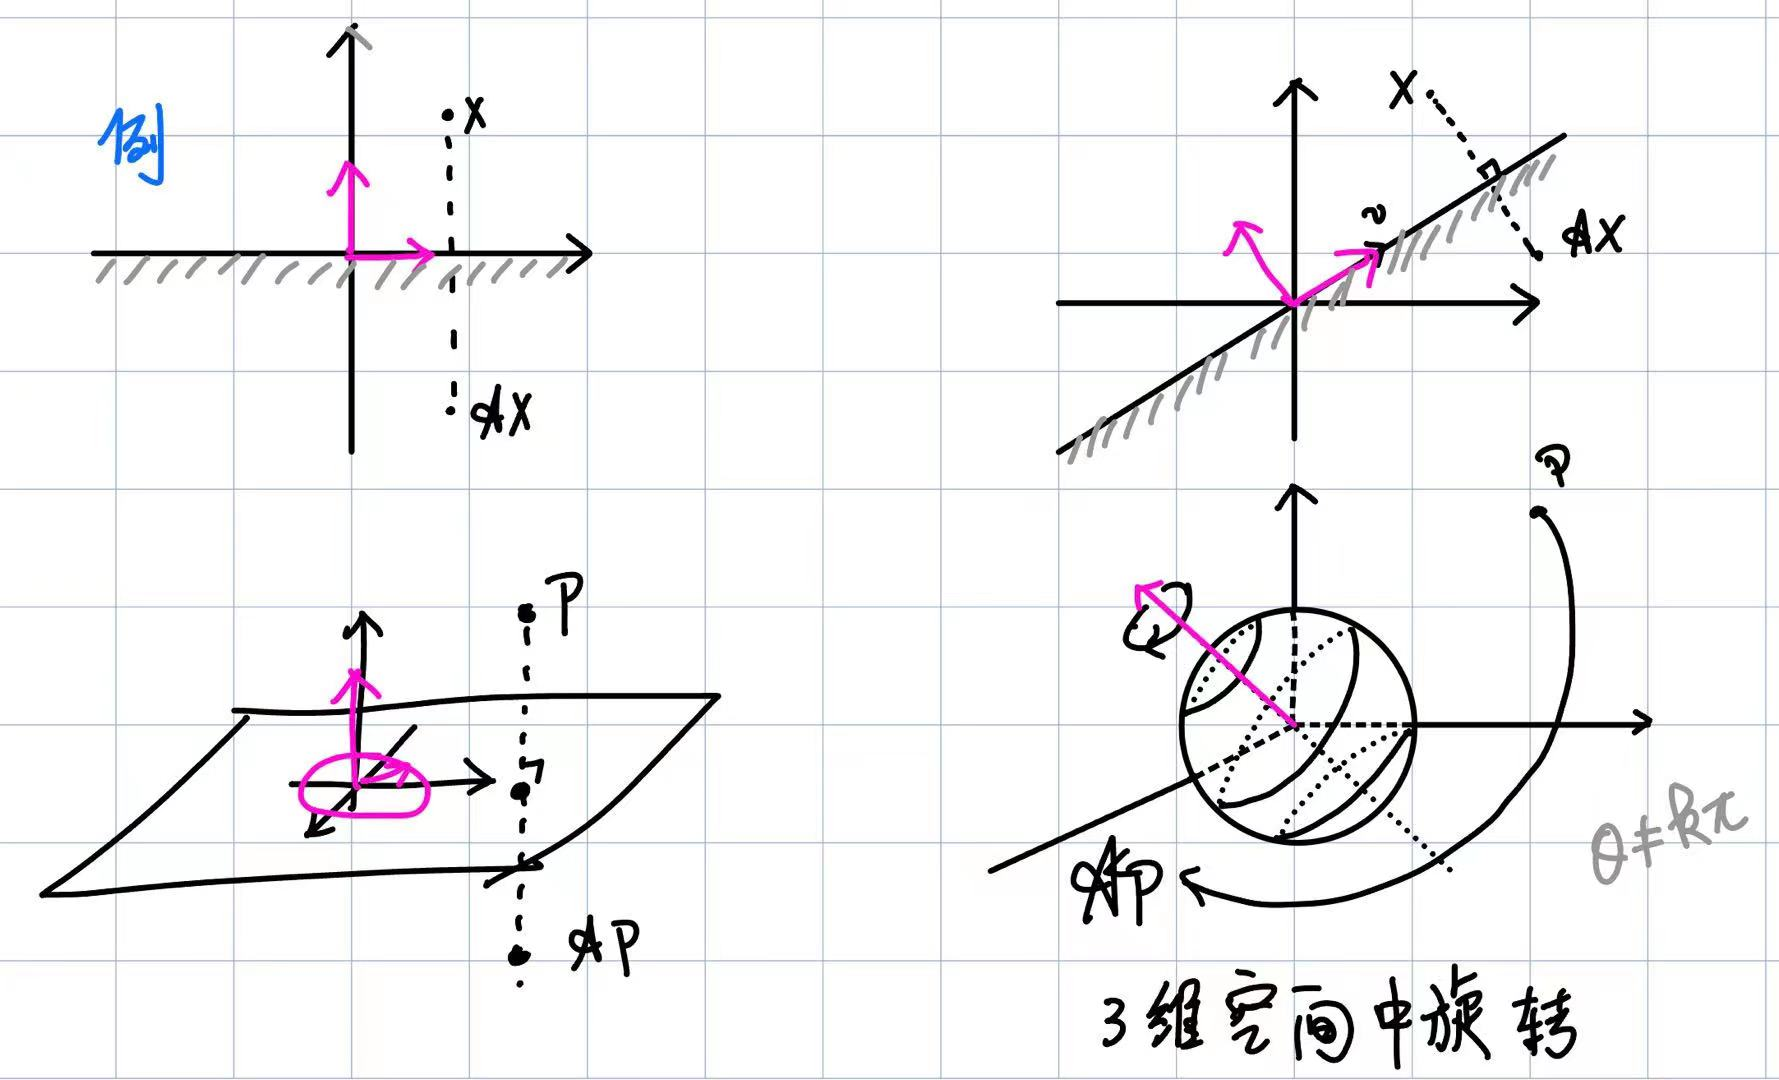
\includegraphics[width=0.6\linewidth]{pic/1e421ae12c6832e0ba34a69ad44cb6b}
\caption{}
\label{fig:1e421ae12c6832e0ba34a69ad44cb6b}
\end{figure}
\end{frame}






\subsubsection{矩阵的特征值和特征向量}
\begin{frame}\frametitle{如何求特征值和特征向量}
\blue{思路:} 通过代数(矩阵)来解决几何问题(特征值,特征向量).

\pp
设$\alpha_1,\cdots,\alpha_n$为$\bF$-线性空间$V$的一组基.
\pp
\begin{center}
\fbox{
$\left\{\text{$V$上的全体}\atop \text{线性变换}\right\}$ \quad $\xleftrightarrow[1:1 \atop \sA(\alpha_1,\cdots,\alpha_n) = (\alpha_1,\cdots,\alpha_n)A]{\text{基} \alpha_1,\cdots,\alpha_n}$ \quad $\bF^{n\times n}$ }
\end{center}
\pp
\begin{definition}[矩阵的特征值,特征向量以及特征子空间]
设$A$为$\bF$系数的$n$阶方阵.
\pp
若存在$\lambda\in F$及\CJKunderdot{非零}数组向量$x\in \bF^n$,使得
\[Ax = \lambda x,\]
\pp
则称$\lambda$为方阵$A$的\blue{特征值},
\pp
称$x$为属于特征值$\lambda$的一个\blue{特征向量}.
\pp
称
\[V_A(\lambda):=\{x\in \bF^n\mid Ax=\lambda x\}\]
为属于$\lambda$的\blue{特征子空间}.
\end{definition}
\end{frame}


\renewcommand{\mydate}{2025年05月15号\ 第二十一次课}


\subsubsection{如何求特征值和特征向量}
\begin{frame}\frametitle{如何求特征值和特征向量}
求$\sA$的特征值和特征向量可以转换为求$A$的特征值和特征向量.
\pp
\begin{proposition}
设$\alpha_1,\cdots,\alpha_n$为$\bF$-线性空间$V$的一组基.
\pp
设$V$上的线性变换在基$\alpha_1,\cdots,\alpha_n$下矩阵为$A$.
\pp
则
\begin{enumerate}
\item $\sA$与$A$有相同的特征值;
\pp
\item 若$\lambda$为$\sA$的特征值,则 $V_\sA(\lambda)=\{(\alpha_1,\cdots,\alpha_n)x\mid x\in V_A(\lambda)\}$.
\end{enumerate}
\end{proposition}
\pp
\yang{\tiny 证明思路: $x\in V_A(\lambda) \Leftrightarrow Ax=\lambda x \Leftrightarrow \sA((\alpha_1,\cdots,\alpha_n)x)=\lambda (\alpha_1,\cdots,\alpha_n)x \Leftrightarrow (\alpha_1,\cdots,\alpha_n)x\in V_{\sA}(\lambda)$.}
\pp
\begin{proposition}
设$\lambda$为方阵$A$的特征值.
\pp
则
\begin{enumerate}
\item $f(\lambda)$为$f(A)$的特征值;
\pp
特别地, $\lambda^k$为方阵$A^k$的特征值;
\pp
\item $\lambda$为方阵$A^T$的特征值;
\pp
\item 若$\lambda\neq0$,则$\frac1\lambda\det(A)$为$A^*$的特征值.
\pp
特别地,若$A$可逆,则$\frac1\lambda$为$A^{-1}$的特征值.
\pp
\item 若$A$为实矩阵且$AA^T=1$,则$|\lambda|=1$.
\end{enumerate}
\end{proposition}
\pp
注:实矩阵的特征值不一定还是实数!
\end{frame}





\subsubsection{矩阵特征值和特征向量一般求解方法}
\begin{frame}\frametitle{矩阵特征值和特征向量一般求解方法}
\begin{example}
求矩阵$A=\begin{pmatrix}1&1\\1&3\end{pmatrix}$的特征值和特征向量.
\end{example}
\pp
\yang{\tiny 解:
$A\left({x\atop y}\right)=\lambda \left({x\atop y}\right)$
\pp
$\Rightarrow$ $\begin{pmatrix}1-\lambda&1\\1&3-\lambda\\\end{pmatrix}\left({x\atop y}\right)=0$
\pp
$\Rightarrow$ $\det \begin{pmatrix}1-\lambda&1\\1&3-\lambda\\\end{pmatrix}=0$
\pp
$\Rightarrow$  $\lambda=2\pm\sqrt{2}$.

\pp
解方程组: $A\left({x\atop y}\right)= 2\pm\sqrt{2}\left({x\atop y}\right)$ 得 $\left({x\atop y}\right)=t\left({1\atop 1\pm\sqrt{2}}\right)$.
}

\pp
对于方阵$A$的特征值的计算,我们有如下一般方法:
\pp
\begin{equation*}
\begin{split}
\text{$\lambda_0$为$A$的特征值}
& \Leftrightarrow  \exists x\neq 0\quad s.t.\ Ax=\lambda_0x\\
\pp
& \Leftrightarrow  \text{线性方程组} (\lambda_0I_n-A)X=0 \text{有非零解}\\
\pp
& \Leftrightarrow  \det(\lambda_0I_n-A)=0\\
\end{split}
\end{equation*}
\pp
即,\fbox{$\lambda_0$为$A$的特征值当且仅当$\lambda_0$为多项式$\det(\lambda I_n-A)$的根.}
\pp
称行列式$\det(\lambda I-A)$为$A$的\blue{特征多项式}.记为\blue{$P_A(\lambda)$}.

\pp
\blue{注:}\begin{enumerate}
\item 数域$\bF$上的多项式在$\bF$上不一定有根!
\pp
\item (代数基本定理) 复数域$\bC$上的非常值多项式在$\bC$上一定有根.
\end{enumerate}
\pp
\yang{在计算特征值和特征向量时,总是假设$\bF=\bC$.}
\end{frame}






\begin{frame}\frametitle{矩阵特征值和特征向量一般求解方法}
设$A$为$n$阶复矩阵.求解过程分为如下两步:
\pp
\begin{enumerate}
\item 求 $P_A(\lambda)=\det(\lambda I_n - A)$,并做分解
\[P_A(\lambda) = (\lambda-\lambda_1)^{n_1}\cdot(\lambda-\lambda_2)^{n_2}\cdot\cdots\cdot(\lambda-\lambda_s)^{n_s}\]
其中$\lambda_i\in\bC$, $n_i\geq1$, $n_1+n_2+\cdots+n_s=n$.
\pp
我们称$n_i$为特征值$\lambda_i$的\blue{重数}.
\pp
\item 给定$i=1,\cdots,s$.解齐次线性方程组 $(\lambda_iI_n-A)X=0$得解空间$V_A(\lambda_i)$或者基础解系.
\end{enumerate}
\pp
\begin{example}
求矩阵$A=\begin{pmatrix}3&-1&-2\\2&0&-2\\2&-1&-1\end{pmatrix}$的特征值和特征向量.
\end{example}
\pp
\yang{答案: $P_A(\lambda)=\lambda(\lambda-1)^2$.
\pp
\begin{itemize}
\item \yang{ $(0\cdot I - A) \vec{x}=0$ $\Rightarrow$ $\vec{x}=c_1\begin{pmatrix}
1\\1\\1\\\end{pmatrix}$;}
\pp
\item \yang{$(1\cdot I - A) \vec{x}=0$ $\Rightarrow$ $\vec{x}=c_2\begin{pmatrix}
1\\2\\0\\\end{pmatrix} + c_3\begin{pmatrix}
0\\-2\\1\\\end{pmatrix}$.}
\end{itemize}
}
\end{frame}






\begin{frame}\frametitle{矩阵特征值和特征向量一般求解方法}
\begin{example}
设$A=\begin{pmatrix}1&1\\0&2\end{pmatrix}$. 设$\sA$为$V=\bF^{2\times 2}$上的线性变换满足$\sA(M)=AM$.
\pp
求$\sA$的特征值和特征向量.
\end{example}
\pp
\yang{答案: $\sA(E_{11},E_{12},E_{21},E_{22}) = (E_{11},E_{12},E_{21},E_{22})B$, 其中$B=\begin{pmatrix}
1&0&1&0\\0&1&0&1\\0&0&2&0\\0&0&0&2\\\end{pmatrix}$.
\pp
$\Rightarrow P_{\sA}(\lambda) =  P_{B}(\lambda) =(\lambda-1)^2(\lambda-2)^2$.
\pp

\begin{itemize}
\item \yang{ $(I_4 - B) \vec{x}=0$ $\Rightarrow$ 基础解系 $\begin{pmatrix}
1\\0\\0\\0\\\end{pmatrix},\begin{pmatrix}
0\\1\\0\\0\\\end{pmatrix}$
\pp
$\Rightarrow$ 特征子空间 $\langle E_{11},E_{12}\rangle$}
\pp
\item \yang{$(2I_4 - B) \vec{x}=0$ $\Rightarrow$ 基础解系$\begin{pmatrix}
1\\0\\1\\0\\\end{pmatrix},\begin{pmatrix}
0\\1\\0\\1\\\end{pmatrix}$
\pp
$\Rightarrow$ 特征子空间 $\langle E_{11}+E_{21},E_{12}+E_{22}\rangle$.}
\end{itemize}
}
\end{frame}





\subsection{相似不变量}

\subsubsection{相似不变量}
\begin{frame}\frametitle{相似不变量}
可以用矩阵来定义线性变换的哪些不变量(即,不依赖于基的选取的量).
\pp
\begin{proposition}
相似的矩阵具有相同的特征多项式和特征值.
\end{proposition}
\pp
\yang{证明:设 $B=T^{-1}AT$.则
\[P_B(\lambda)=\det(\lambda I-T^{-1}AT)=\det(T^{-1})\det(\lambda I-A)\det(T)=P_A(\lambda).\]}
\pp
即,可以用矩阵来定义线性变换的特征多项式和特征值.
\pp
有没有其它相似不变量呢?
\begin{theorem}
设$A$为$n$阶复矩阵的$n$个特征值分别为$\lambda_1,\cdots,\lambda_n$(可能有重复的).
\pp
则
\begin{enumerate}
\item $\mathrm{tr}(A)=\sum_{i=1}^{n}\lambda_i$;
\pp

\item $\det(A)=\lambda_1\lambda_2\cdots\lambda_n$.
\end{enumerate}
\end{theorem}
\pp
\yang{证明思路:展开$P_A(\lambda)$并使用根与系数之间的关系.}
\pp
\begin{corollary}
一个$n$阶方阵可逆当且仅当其$n$个特征值均不为零.
\end{corollary}
\end{frame}









% ========== 2023年05月25号 第24次课 相似对角化 ==========
%\frame{\titlepage}





\subsubsection{相似不变量的应用}
\begin{frame}\frametitle{相似不变量的应用}
\begin{example}
设$n$阶方阵$A$的全体特征值为$\lambda_1,\lambda_2,\cdots,\lambda_n$.
\pp
\begin{itemize}
\item 求$I+A$的全体特征值和行列式;
\pp
\item 更一般地,求矩阵$f(A)$的全体特征值.
\end{itemize}
\end{example}
\pp
\yang{解题思路: $P_{I+A}(\lambda)=P_A(\lambda-1)$.
\pp
 设$\lambda-f(x)=a_0\prod\limits_{i=1}^d (\alpha_i-x)$.
\pp
则
\begin{equation*} \tiny
\begin{split}
\det\left(\lambda I- f(A)\right) & = \det\left(a_0\prod_{i=1}^d(\alpha_i I-A)\right)
\pp
= a_0^n\prod_{i=1}^d\det(\alpha_i I-A) \\
\pp
& = a_0^n \prod_{i=1}^d \prod_{j=1}^n(\alpha_i-\lambda_j)
\pp
= \prod_{j=1}^n \left(a_0\prod_{i=1}^d (\alpha_i-\lambda_j)\right)
\pp
= \prod_{j=1}^n(\lambda - f(\lambda_j))\\
\end{split}
\end{equation*}
}

\pp
\begin{example}
若$A=\begin{pmatrix}1&0&0\\0&0&1\\0&1&x\end{pmatrix}$和$B=\begin{pmatrix}y&0&0\\0&-1&1\\0&0&1\end{pmatrix}$相似.求$x,y$.
\end{example}
\pp
提示:相似不变量.
\end{frame}



\subsection{相似对角化}

\subsubsection{矩阵的相似对角化}
\begin{frame}\frametitle{矩阵的相似对角化}

现在我们回到原始问题: 哪些线性变换由伸缩给出?
\pp
\begin{definition}[可对角化]
相似于对角矩阵的方阵称为\blue{可对角化}的.
\pp
我们称一个线性变换为\blue{可对角化}的,若它在某组基下的矩阵可对角化.
\end{definition}
\pp
\blue{问题:} 如何判断一个线性变换是否可对角化.
\pp
\begin{example}[不是所有的线性变换和矩阵都可对角化]
$A=\begin{pmatrix}
2&1\\0&2\\\end{pmatrix}$.
\end{example}
\end{frame}






\renewcommand{\mydate}{2025年05月20号\ 第二十二次课}



\subsubsection{可对角化的判定准则}
\begin{frame}\frametitle{可对角化的判定准则}
若 $ A=T\mathrm{diag}(\lambda_1,\cdots,\lambda_n)T^{-1}$. 记$T=(\eta_1,\cdots,\eta_n)$.
\pp
则
\begin{enumerate}
\item $\eta_1,\cdots,\eta_n$线性无关,
\pp
\item $A\eta_i=\lambda_i\eta_i$.
\end{enumerate}
\pp
\begin{theorem}[利用特征向量来判定]
方阵$A$可对角化 $\Leftrightarrow$ $A$有$n$个线性无关的特征向量.
\end{theorem}
\pp
\yang{有没有简单一点的办法来判断呢?

\pp
有时候,可以用相似不变量来判断.(不需要求特征向量!)}
\pp
\begin{lemma}
属于不同特征值的特征向量线性无关.
\pp 即,若$\lambda_1,\cdots,\lambda_k$为方阵$A$的两两不同的特征值,$\eta_i$为属于$\lambda_i$的特征向量,则$\eta_1,\cdots,\eta_k$线性无关.
\end{lemma}
\pp
\yang{证明思路:范德姆行列式不为零!}
\pp
\begin{corollary}[利用特征值来判定]
若$n$阶方阵有$n$个两两不同的特征值,则$A$可对角化.
\end{corollary}
\pp
\yang{优点:不需要求解特征向量; 缺点:不是充要条件,有重根咋办?}
\end{frame}





\subsubsection{利用重数*}
\begin{frame}\frametitle{重数*}
一般地,我们可以用特征值的重数来判定是否可对角化.
\pp
\begin{definition}[代数重数,几何重数]
设$A$为$n$阶复矩阵的特征多项式有分解
\[P_A(\lambda) = (\lambda-\lambda_1)^{n_1}(\lambda-\lambda_2)^{n_2}\cdots(\lambda-\lambda_s)^{n_s}.\]
\pp
称$n_i$为$\lambda_i$的\blue{代数重数},
\pp
称子空间$V_A(\lambda_i)$的维数为$\lambda_i$的\blue{几何重数}.
\end{definition}
\pp
\begin{theorem}[利用特征值的重数来判定]
\begin{enumerate}
\item $1\leq$ 几何重数 $\leq$ 代数重数.
\pp
\item $A$可对角化 $\Leftrightarrow$ 每个特征值的几何重数与代数重数相等.
\end{enumerate}
\end{theorem}
\pp
\yang{证明思路:将$V_A(\lambda_i)$的一组基扩充为整个空间的一组基.}
\end{frame}






\begin{frame}\frametitle{重数*}

\begin{example}
什么时候$A=\begin{pmatrix}0&0&x\\1&1&y\\1&0&0\end{pmatrix}$可对角化?
\end{example}
\pp
\yang{
解题思路: $P_A(\lambda)=(\lambda-1)(\lambda^2-x)$.
\pp
\begin{itemize}
\item \yang{$x\neq 0,1$ $\Rightarrow$ 三个不同特征值.}
\pp
\item \yang{$x=0$  $\Rightarrow$  $0$的代数重数为$2$而几何重数为$1$.}
\pp
\item \yang{$x=1$  $\Rightarrow$  $-1$的重数为$1$. $1$的代数重数为$2$,几何重数为$2$($y=-1$)或者$1$($y\neq-1$).}
\end{itemize}
}
\end{frame}



\renewcommand{\mydate}{2025年05月22号\ 第二十三次课}


\subsubsection{利用极小多项式*}
\begin{frame}\frametitle{极小多项式*}
\begin{theorem}[哈密尔顿-凯莱定理]
$P_A(A)=0$.
\end{theorem}
\pp
特别地,任意方阵$A$都存在零化多项式.称次数最小的首一零化多项式为$A$的\blue{极小多项式}.
(注:极小多项式为相似不变量.)
\pp
\begin{proposition}
\begin{enumerate}
\item 极小多项式整除其他任意零化多项式.特别地,极小多项式为特征多项式的因子.
\pp
\item 一个数为特征值当且仅当其为极小多项式的根.
\end{enumerate}
\end{proposition}
\pp
\begin{theorem}[利用极小多项式]
方阵可对角化当且仅当其极小多项式无重根.
\end{theorem}
\pp
%\yang{证明思路: 设极小多项式为$\prod\limits_{i=1}^d(x-\lambda_i)$,记 $f_j(x)=\prod\limits_{j=1\atop j\neq i}^d(x-\lambda_j)$ 以及 $V_i:=V_A(\lambda_i)$. 我们仅需证明$\bF^n=\bigoplus_{i} V_i$.
%
%存在多项式$g_1(x),\cdots,g_d(x)$使得
%$1=\sum_{j=1}^d f_i(x)g_i(x)$.
%}
\begin{corollary}[利用零化多项式]
方阵可对角化当且仅当其存在无重根的零化多项式.
\end{corollary}
\pp
\blue{例:} 设方阵 $A$满足 $A^2=A$, $A^2=I$ 或 $A^3=A$ 等.则$A$可对角化.
\end{frame}









% ========== 2023年05月30号 第25次课 上三角化,若当标准形 ==========
%\frame{\titlepage}


\subsection{相似上三角化与若当标准形}


\subsubsection{相似上三角化}
\begin{frame}\frametitle{相似上三角化}
不是每个矩阵都可以对角化,但总是可上三角化!
\pp
\begin{theorem}
\begin{enumerate}
\item 任意$n$阶复方阵$A$都相似于一个上三角形矩阵$J$,
\pp
且
\item $J$的对角线上的元素为$A$的全体特征值.
\end{enumerate}
\end{theorem}
\pp
\yang{证明思路:将$A$的一个特征向量$\xi_1$扩充为$\bC^n$的一组基$\xi_1,\cdots,\xi_n$,并记组成的可逆矩阵$(\xi_1,\cdots,\xi_n)$为$P$.
\pp
则
\[AP=P\begin{pmatrix} \lambda & * \\ & A_{22}
\end{pmatrix}.\]
\pp
对矩阵阶数归纳,不妨设$A_{22}=Q\begin{pmatrix}\lambda_2&&*\\&\ddots&\\&&\lambda_n\\\end{pmatrix}Q^{-1}$.
\pp
则
\[A= P\begin{pmatrix} 1 &  \\ & Q\end{pmatrix} \cdot \begin{pmatrix}\lambda_1&&*\\&\ddots&\\&&\lambda_n\\\end{pmatrix} \left(P\begin{pmatrix} 1 &  \\ & Q\end{pmatrix} \right)^{-1}.\]
}

\pp
\blue{注:} $J$的取法不唯一.(例:${0\ 1\choose0\ 0}$和${0\ 2\choose0\ 0}$.)

\pp
\blue{例:} 若复二阶矩阵$A$满足$A^2=0$,则$A=0$或者$A$相似于${0\ 1\choose0\ 0}$.
\end{frame}






\subsubsection{若当矩阵*}
\begin{frame}\frametitle{若当矩阵*}
相似等价类中的最简代表元是什么?
\pp
为了回答这一问题,我们需要引进:
\begin{definition}[若当块,若当矩阵]
\pp
\begin{enumerate}
\item 给定任意正整数$m$和复数$\lambda$. 称矩阵 $J_m(\lambda)=\begin{pmatrix}
\lambda&1&&\\&\lambda&\ddots&\\
&&\ddots&1\\&&&\lambda\\\end{pmatrix}$为\blue{若当块}.
\pp
\item 称由若当块组成的对角分块矩阵 $J=\begin{pmatrix}
J_{m_1}(\lambda_1)&&&\\&J_{m_2}(\lambda_2)&&\\
&&\ddots&\\&&&J_{m_s}(\lambda_s)\\\end{pmatrix}$为\blue{若当矩阵}.
\end{enumerate}
\end{definition}
\end{frame}





\subsubsection{相似等价类中的最简代表元(若当标准形)*}
\begin{frame}\frametitle{相似等价类中的最简代表元(若当标准形)*}
\begin{theorem}
\begin{enumerate}
\item 任意复方阵都与某若当矩阵相似,
\pp
并且
\item 不计若当块排序下,这个若当矩阵取法唯一.
\pp
称之为给矩阵的\blue{若当标准形}
\end{enumerate}
\end{theorem}
\pp
\begin{example}
设$\lambda$为$5$阶复矩阵$A$的$5$重特征值.请分析$A$的若当标准形.
\end{example}
\pp
\begin{example}
求矩阵$A=\begin{pmatrix}3&-2&1\\2&-2&2\\3&-6&5\end{pmatrix}$的若当标准形.
\end{example}

\yang{\[T^{-1}AT = \begin{pmatrix}2&1&\\&2&\\&&2\\\end{pmatrix}, \qquad T = \begin{pmatrix}
1 & 1 & -1 \\ 2 & 0 & 0 \\ 3 & 0 & 1 \\ \end{pmatrix}.\]}
\end{frame}





\subsubsection{若当标准形在求解常微分方程组上的一个应用*}
\begin{frame}\frametitle{若当标准形在求解常微分方程组上的一个应用*}
利用若当标准形, 可完全解决常系数线性微分方程组的求解问题.

\pp

\begin{example}
设$x,y,z$都是$t$的函数，求解常微分方程组
\begin{equation*}
\begin{cases}
\frac{\mathrm{d}x}{\mathrm{d}t}  = 3x - 2y + \ z\\
\frac{\mathrm{d}y}{\mathrm{d}t}  = 2x - 2y + 2z\\
\frac{\mathrm{d}z}{\mathrm{d}t}  = 3x - 6y + 5z\\
\end{cases}
\end{equation*}
\end{example}
\pp
\bigskip


改写原方程组为 $\frac{\mathrm{d}\mathbf{x}}{\mathrm{d}t} = A\mathbf{x}$. 作线性代换 $\mathbf{x} = T\mathbf{x}^*$, 则
\[\frac{\mathrm{d}\mathbf{x}^*}{\mathrm{d}t} = T^{-1}AT\mathbf{x}^*. \quad \text{ 即, } \quad
\begin{cases}
\frac{\mathrm{d}x^*}{\mathrm{d}t} = 2x^* + y^* \\
\frac{\mathrm{d}y^*}{\mathrm{d}t} = 2y^* \\
\frac{\mathrm{d}z^*}{\mathrm{d}t} = 2z^*
\end{cases}
\]
解此方程组得 $z^* = c_1e^{2t},\ y^* = c_2e^{2t},\ x^* = (c_2t + c_3)e^{2t}.$
再利用 $\mathbf{x} = T\mathbf{x}^*$, 即得到通解是
\[
\begin{cases}
x(t) = (c_2t + c_2 + c_3 - c_1)e^{2t} \\
y(t) = (2c_2t + 2c_3)e^{2t}  \qquad \text{其中 $c_1, c_2, c_3$ 为任意常数.}\\
z(t) = (3c_2t + 3c_3 + c_1)e^{2t}
\end{cases}
\]







\end{frame}






\renewcommand{\mydate}{2025年05月27日\ 二十四次课}


%\setcounter{framenumber}{30}
\makeatletter
\ifodd\value{page}
\else
\begin{frame}[plain]
\end{frame}
\fi
\makeatother


\section{内积空间及变换}

\title{第八章 \quad 内积空间及变换}
\author{}
\date{}

\frame{\titlepage}

\subsection{欧氏空间的定义}

\subsubsection{距离与夹角}
\begin{frame}\frametitle{距离与夹角}
三维空间中有距离,夹角等概念 $\xRightarrow{\text{坐标系}}$ 三维数组向量空间$\bR$上向量的模长和夹角.
\pp

比较容易地推广到$\bR^n$: $|(x_1,\cdots,x_n)|:=\sqrt{x_1^2+\cdots+x_n^2}$.
\pp

问题: 如何推广到抽象的线性空间上呢?
\pp
\begin{table}[]
\begin{tabular}{||r||c||l||}\hline\hline
线性空间 & $\xleftrightarrow[1:1]{\text{基} \alpha_1,\cdots,\alpha_n}$ & $\bR^n$ \\ \hline\hline
向量$v$ & $\longleftrightarrow$ & 坐标 \\ \hline
线性变换$\sA$ & $\longleftrightarrow$ & A \\ \hline
?? & $\longleftrightarrow$ & 长度,夹角 \\ \hline
$\sA$(保持长度) & $\longleftrightarrow$ & ?? \\\hline
$\sA$(??) & $\longleftrightarrow$ & 转置矩阵 \\ \hline
$\sA$(??) & $\longleftrightarrow$ & 对称矩阵 \\ \hline\hline
\end{tabular}
\end{table}
\end{frame}






\begin{frame}\frametitle{距离与夹角}
回顾$\bR^3$上的模长与夹角公式:
\pp
\begin{equation*}
\begin{split}
|a| & = \sqrt{(a,a)}\\
\pp
\theta & = \arccos\frac{(a,b)}{\sqrt{(a,a)(b,b)}}
\end{split}
\end{equation*}
\pp
容易看出模长和夹角可以由内积完全确定.
\pp
反之,内积可由模长唯一确定
\[(a,b)=\frac{|a+b|^2-|a|^2-|b|^2}{2}.\]
\pp
总结 $\bR^3$上内积有如下基本性质:
\begin{enumerate}
\item 对称性
\item 线性性
\item 正定性
\end{enumerate}
\pp
\yang{为了在一般的$\bR$-线性空间上定义度量,我们需要引入一般空间上的内积.}
\end{frame}








\subsubsection{欧氏空间的定义}
\begin{frame}\frametitle{欧氏空间的定义}
\begin{definition}[内积,欧氏空间]
\pp
设$V$为有限维$\bR$-线性空间.
\pp
若存在一个映射$(-,-)\colon V\times V \rightarrow \bR$满足:
\pp
\begin{enumerate}
\item 对称性: $(a,b)=(b,a)$;
\pp
\item 双线性: $(\lambda a,b)=\lambda(a,b)$, $(a+b,c)=(a,c)+(b,c)$;
\pp
\item 正定性: $(a,a)\geq0$,且等号成立当且仅当$a=0$,
\end{enumerate}
\pp
则称$(a,b)$为$a$和$b$的\blue{内积}.
\pp 带内积的$\bR$-线性空间称为\blue{欧氏空间}(或,\blue{欧几里得空间}).
\end{definition}
\pp
\begin{center}
欧式空间 = $\bR$-线性空间 + 内积;\\
$\bR$-线性空间 = 集合 + 加法 + ($\bR$)数乘\\
\end{center}
\pp
注: 内积$(-,-)$对第二个分量也是线性的.
\pp
\begin{proposition}[内积的基本性质]
\begin{enumerate}
\item $\left(\sum_{i=1}^{k}\lambda_ia_i,\sum_{j=1}^{m}\mu_jb_j\right) = \sum_{i=1}^{k}\sum_{j=1}^{m} \lambda_i\mu_j(a_i,b_j)$;
\pp
\item $(a,0)=0$;
\pp
\item 内积结构由一组基之间的内积完全确定.
\end{enumerate}
\end{proposition}
\end{frame}





\subsubsection{模长与夹角}
\begin{frame}\frametitle{模长与夹角}
\pp

为了定义夹角,我们需要引入:

\begin{theorem}[Cauchy-Schwarz 不等式]
\pp
设$V$为欧式空间. 对于任意$a,b\in V$,我们有
\[|(a,b)|\leq \sqrt{(a,a)\cdot(b,b)}.\]
\end{theorem}
\pp
\yang{证明思路:考虑二次多项式$(xa+b,xa+b)$的判别式.}

\pp
\yang{可以定义夹角了!(不确定原理.)}
\pp
\begin{definition}[长度,夹角]
设$V$为欧氏空间. 对于任意向量 $a,b\in V$,
\begin{enumerate}
\item 称$|a|:=\sqrt{(a,a)}$为$a$的\blue{长度}(或,\blue{模长});
\pp
\item 称$|a-b|$为$a$和$b$之间的\blue{距离}.记为\blue{$d(a,b)$}.
\pp
\item 若$a,b$不为零,定义$a$和$b$之间的\blue{夹角}为 $\theta = \arccos\frac{(a,b)}{|a|\cdot|b|}$.
\pp
特别地,当$(a,b)=0$时,称$a$与$b$\blue{正交}或\blue{垂直},记为 \blue{$a\perp b$}.
\pp
\item 称$a$为\blue{单位向量},若$|a|=1$.
\pp
若$b\neq0$,称$\frac{1}{|b|}b$为$b$的\blue{单位化}.
\end{enumerate}
\end{definition}
\end{frame}





\subsubsection{距离基本性质}
\begin{frame}\frametitle{距离基本性质}
\pp
\begin{proposition}
\begin{enumerate}
\item 对称性: $d(a,b)=d(b,a)$;
\pp
\item 正定性: $d(a,b)\geq0$, 等号成立当且仅当$a=b$;
\pp
\item 三角不等式: $d(a,c)\leq d(a,b)+ d(b,c)$;
\pp
\item 勾股定理: $a\perp b$ 当且仅当 $|a|^2+|b|^2=|a+b|^2$;
\pp
\item 菱形定理: 若$|a|=|b|$,则$(a+b)\perp(a-b)$.
\end{enumerate}
\end{proposition}
\end{frame}





\begin{frame}\frametitle{内积的基本例子}
\pp
\begin{example}
设$V=\bR^n$,对于任意两向量 $a=(a_1,\cdots,a_n)$和 $b=(b_1,\cdots,b_n)$, 定义
\[(a,b)=a_1b_1+\cdots+a_nb_n.\]
\pp
则$(-,-)$为$V$上的一个内积.这一内积给出通常的模长和夹角.
\pp
此时Cauchy-Schwarz公式为
\[\left(\sum_{i=1}^n a_ib_i\right)^2 \leq \left(\sum_{i=1}^n a_i^2\right)\cdot\left(\sum_{i=1}^n b_i^2\right).\]
\end{example}
\pp
\begin{example}
类似的$(a,b)=a_1b_1+2a_2b_2+\cdots+na_nb_n$也可以定义$V=\bR^n$上的一个内积.
\end{example}
\end{frame}






\begin{frame}\frametitle{内积的基本例子}

\yang{构造一个内积使得给定的一组基均为单位向量且两两垂直.}
\pp
\begin{example}
设$\alpha_1,\cdots,\alpha_n$为$n$维$\bR$-线性空间$V$上的一组基.
\pp
对于任意向量$\alpha,\beta\in V$,定义
\[(\alpha,\beta)=a_1b_1+a_2b_2+\cdots+a_nb_n,\]
其中$(a_1,a_2,\cdots,a_n)$和$(b_1,b_2,\cdots,b_n)$分别为$\alpha$和$\beta$在基$\alpha_1,\cdots,\alpha_n$下的坐标.
\pp
则$(-,-)$为$V$上的内积.在此内积下$\alpha_1,\cdots,\alpha_n$均为单位向量且两两垂直.
\pp
即,
\[(\alpha_i,\alpha_j)=\delta_{ij}=\left\{\begin{array}{ll}
1,& i=j;\\
0,& i\neq j.\\
\end{array}\right.\]
\end{example}
\pp
\yang{任意有限维实线性空间一定存在内积. 注:任意内积均为这一形式!}
\end{frame}




\subsubsection{Hilbert空间*}
\begin{frame}\frametitle{Hilbert空间*}

在无穷维空间上也可类似的定义内积.
\pp
\begin{example}[无限维空间上的内积]
对应任意$[a,b]$上的连续函数$f,g\in C[a,b]$,定义
\[(f,g):=\int_a^b f(x)g(x)\mathrm{d}x.\]
\pp
类似地,定义连续函数的模长,夹角和正交等概念.此时Cauchy-Schwarz公式为
\[\left(\int_a^b f(x)g(x)\mathrm{d}x\right)^2\leq\left(\int_a^b f(x)^2\mathrm{d}x\right)\cdot\left(\int_a^b g(x)^2\mathrm{d}x\right).\]
\pp
当$a=-\pi$,$b=\pi$时,三角函数$1,\cos x,\sin x,\cos2x,\sin2x,\cdots$在这一内积下两两正交.
\end{example}
\pp
我们称带内积\blue{完备的}$\bR$-线性空间为\blue{Hilbert空间}.

\end{frame}



\subsection{度量矩阵(内积的矩阵表示)}

\subsubsection{内积的矩阵表示}
\begin{frame}\frametitle{内积的矩阵表示}
\pp
设$\alpha_1,\cdots,\alpha_n$为欧氏空间$V$的一组基.
\pp
任取$\alpha = a_1\alpha_1+\cdots+a_n\alpha_n$, $\beta = b_1\alpha_1+\cdots+b_n\alpha_n\in V$,则
\begin{equation}\label{equ:innerprod}
(\alpha,\beta)=\sum_{i=1}^n\sum_{j=1}^n a_ib_j(\alpha_i,\alpha_j).
\end{equation}
\pp
因此内积$(-,-)$由值$g_{ij}:=(\alpha_i,\alpha_j)$($1\leq ij\leq n$)唯一确定.
\pp
记
\[G:=(g_{ij})_{n\times n}.\]
称$G$为内积$(-,-)$在基$\alpha_1,\cdots,\alpha_n$下的\blue{度量矩阵}.
\pp
记
\[x=\begin{pmatrix}a_1\\\vdots\\a_n\end{pmatrix},y=\begin{pmatrix}b_1\\\vdots\\b_n\end{pmatrix}\]
则\eqref{equ:innerprod}可简写为
\[\blue{(\alpha,\beta)=x^TGy.}\]
\end{frame}


\renewcommand{\mydate}{2025年05月29日\ 二十五次课}



\begin{frame}\frametitle{}
通过度量矩阵我们有如下映射
\begin{equation*}
\xymatrix@C=2cm@R=0cm{
\text{$V$上的内积}
\ar[r]^-{\text{基}\alpha_1,\cdots,\alpha_n}	& \bR\text{上的$n$阶矩阵} \\
(-,-) \ar@{|->}[r] & G=\Big((\alpha_i,\alpha_j)\Big)_{n\times n} \\
}
\end{equation*}
\pp

\yang{问题: 哪些矩阵落在这个映射的像集里面?即,哪些矩阵能够成为某个内积的度量矩阵?}
\pp

\begin{proposition}[度量矩阵的基本性质]
\begin{enumerate}
\item 设$G$为$V$上某内积$(-,-)$在基$\alpha_1,\cdots,\alpha_n$下的度量矩阵.
\pp
则
\begin{itemize}
\item $G$为实对称矩阵;
\pp
\item 对任意$x\in\bR^n$,都有$x^TGx\geq0$,且等号成立当且仅当$x=0$.
\end{itemize}
\pp
称满足如上性质的矩阵为\blue{正定矩阵}.
\pp
因此内积的度量矩阵为正定矩阵.
\pp
\item 反之,对于任意给定的正定矩阵$G$, 通过
\[(\alpha,\beta):=x^TGy\]
可以构造出$V$上的一个内积,其中$x,y$为$\alpha$和$\beta$的坐标.
\end{enumerate}
\end{proposition}
\end{frame}






\begin{frame}\frametitle{}
\yang{问题:
\begin{enumerate}
\item 不同基下度量矩阵之间的关系?
\pp
\item 度量矩阵的最简形式,在哪组基下度量矩阵为最简单形式?
\end{enumerate}
}
\pp
\begin{proposition}
设$P$为欧氏空间的两组基$\alpha_1,\cdots,\alpha_n$和$\eta_1,\cdots,\eta_n$为之间的过渡矩阵
\[(\eta_1,\cdots,\eta_n) = (\alpha_1,\cdots,\alpha_n)P.\]
\pp
设内积在$\alpha_1,\cdots,\alpha_n$和$\eta_1,\cdots,\eta_n$下的度量矩阵为$G$和$\overline{G}$. 即,
\[G=\Big((\alpha_i,\alpha_j)\Big)_{n\times n},\quad \overline{G}=\Big((\eta_i,\eta_j)\Big)_{n\times n}.\]
\pp
则
\[\overline{G}=P^TGP.\]
\end{proposition}
\pp
\yang{证明思路: $\overline{G}_{(i,j)}=(\eta_i,\eta_j)=\left(\sum\limits_{s=1}^{n}p_{si}\alpha_s,\sum\limits_{t=1}^{n}p_{tj}\alpha_t\right)=\sum\limits_{s=1}^n\sum\limits_{t=1}^n p_{si}G_{(s,t)} p_{tj} = (P^TGP)_{(i,j)}$.}
\end{frame}





\subsubsection{相合关系及其基本性质}
\begin{frame}\frametitle{相合关系及其基本性质}
\begin{definition}[相合]
称两个矩阵$G$和$\overline{G}$ \blue{相合},若存在可逆阵$P$使得
\[\overline{G}=P^TGP.\]
\end{definition}
\pp
\begin{proposition}
\begin{enumerate}
\item 内积在不同基下的度量矩阵相合;
\pp
\item 相合为等价关系.
\end{enumerate}
\end{proposition}
\pp
实对称矩阵的相合分类,以及相合标准形(第八章).

\end{frame}




\subsection{标准正交基}


\subsubsection{标准正交基}
\begin{frame}\frametitle{标准正交基}
\yang{度量矩阵的最简形式?为了回答这一问题,我们需要引入标准正交基.}

\pp
\begin{definition}[标准正交基]
设$V$为$n$维欧氏空间.
\begin{enumerate}
\item 称由一组两两正交的非零向量为\blue{正交向量组};
\pp
\item 称由正交向量组构成的基为\blue{正交基};
\pp
\item 称由单位向量组成的正交基为\blue{标准正交基}.
\end{enumerate}
\end{definition}
\pp
\begin{example}设$(-,-)$为$\bR^n$上的一内积.
\pp
\begin{enumerate}
\item 若$((x_1,\cdots,x_n),(y_1,\cdots,y_n))=\sum_{i=1}^nx_iy_i$.
\pp
则自然基
\[e_1,\cdots,e_n\]
为一组标准正交基.
\pp
\item 若$((x_1,\cdots,x_n),(y_1,\cdots,y_n))=\sum_{i=1}^nix_iy_i$.
\pp
则
\[e_1,\frac{e_2}{\sqrt{2}}\cdots,\frac{e_n}{\sqrt{n}}\]
为一组标准正交基.
\end{enumerate}
\end{example}
\end{frame}









% ========== 2023年06月06号 第27次课 标准正交基,正交变换 ==========
%\frame{\titlepage}






\begin{frame}\frametitle{标准正交基}
\yang{度量矩阵的最简形式?为了回答这一问题,我们需要引入标准正交基.}

\begin{definition}[标准正交基]
设$V$为$n$维欧氏空间.
\begin{enumerate}
\item 称由一组两两正交的非零向量为\blue{正交向量组};
\item 称由正交向量组构成的基为\blue{正交基};
\item 称由单位向量组成的正交基为\blue{标准正交基}.
\end{enumerate}
\end{definition}

\begin{proposition}
正交向量组线性无关.
\end{proposition}
\pp

\begin{theorem}[标准正交基使度量矩阵最简]
设$V$为$n$维欧氏空间. 设$G$为内积在基$\alpha_1,\cdots,\alpha_n$下的度量矩阵.
\pp
则
\begin{center}
$\alpha_1,\cdots,\alpha_n$为标准正交基 \quad $\Leftrightarrow$ \quad $G=I_n$.
\end{center}
\end{theorem}
\pp
下面将讨论标准正交基的存在性.
\end{frame}





\subsubsection{Schmidt正交化}
\begin{frame}\frametitle{Schmidt正交化}

\begin{theorem}[Schmidt正交化]
给定欧氏空间的任意一组基$\alpha_1,\cdots,\alpha_n$,则存在一组标准正交基$e_1,\cdots,e_n$使得(对所有的$i=1,2,\cdots,n$)
\[\langle\alpha_1,\cdots,\alpha_i\rangle = \langle e_1,\cdots,e_i\rangle.\footnote{\text{也等价于 $(\alpha_1,\cdots,\alpha_i) = (e_1,\cdots,e_i)R$, 其中$R$为可逆上三角矩阵.}}\]

\end{theorem}
\pp
\yang{几何解释?}
\yang{证明思路: 递归地定义 $\beta_k=\alpha_k - \sum_{i=1}^{k-1}(\alpha_k,e_i)e_i\neq0$ 以及 $e_k=\frac{\beta_k}{|\beta_k|}$.}
\pp

\begin{corollary}[实可逆阵的QR分解]
对任意可逆实矩阵 $A$, 存在方阵$Q$和上三角矩阵$R$使得$A=QR$, 其中$Q$的列向量构成$\mathbb R^n$的标准正交基.
\end{corollary}
\end{frame}



\renewcommand{\mydate}{2025年06月03日\ 二十六次课}


\begin{frame}\frametitle{Schmidt正交化}
\begin{example}
将
$\alpha_1=\begin{pmatrix}1\\1\\0\\0\end{pmatrix}$,
$\alpha_2=\begin{pmatrix}1\\0\\1\\0\end{pmatrix}$,
$\alpha_3=\begin{pmatrix}-1\\0\\0\\1\end{pmatrix}$,
$\alpha_4=\begin{pmatrix}1\\-1\\-1\\0\end{pmatrix}$标准正交化.
\end{example}
\pp
\begin{corollary}
对任意正定矩阵$A$,存在可逆实矩阵$P$使得$A=P^TP$.
\end{corollary}
\end{frame}



\subsection{正交变换}

\subsubsection{正交变换}
\begin{frame}\frametitle{正交变换}
\begin{table}[]
\begin{tabular}{||r||c||l||}\hline\hline
$n$维欧氏空间 & $\xleftrightarrow[1:1]{\text{标准正交基基} \alpha_1,\cdots,\alpha_n}$ & $\bR^n$(带标准内积) \\ \hline\hline
线性变换$\sA$ & $\xleftrightarrow[1:1]{\sA(\alpha_1,\cdots,\alpha_n)=(\alpha_1,\cdots,\alpha_n)A}$ & 矩阵A \\ \hline
$\sA$(保持内积) & $\longleftrightarrow$ & ?? \\\hline
\end{tabular}
\end{table}

\pp
\begin{example}空间(平面)的旋转和镜面反射等.
\end{example}
\pp

\begin{definition}[正交变换]
设$\sA$为欧氏空间$V$上的线性变换.若$\sA$ \CJKunderdot{保持内积},即(对任意$a,b\in V$,
\[(\sA a,\sA b)=(a,b),\]
则称$\sA$为\blue{正交变换}.
\end{definition}
\end{frame}





\subsubsection{正交变换的等价刻画}
\begin{frame}\frametitle{正交变换的等价刻画}
\pp
\begin{theorem}
设$\sA$为欧氏空间$V$上的线性变换.则以下几条等价
\begin{enumerate}
\item $\sA$ 正交;
\pp
\item $\sA$ 保持向量长度;
\pp
\item $\sA$ 将标准正交基变为标准正交基.
\end{enumerate}
\end{theorem}
\pp
\yang{\tiny 证明思路:(1)$\Leftrightarrow$(2) \& (1)$\Leftrightarrow$(3)

\pp
(1)$\Rightarrow$(2): $|\sA(\alpha)|=\sqrt{(\sA(\alpha),\sA(\alpha))}=\sqrt{(\alpha,\alpha)}=|\alpha|;$
\pp

(2)$\Rightarrow$(1): $(\sA(\alpha),\sA(\beta)) = \frac{|\sA(\alpha+\beta)|^2-|\sA(\alpha)|^2-|\sA(\beta)|^2}{2}$
\[= \frac{|\alpha+\beta|^2-|\alpha|^2-|\beta|^2}{2}
=(\alpha,\beta)\]
\pp
(1)$\Rightarrow$(3):
$e_1,\cdots,e_n$ = 标准正交基 $\Rightarrow$ $(\sA(e_i),sA(e_j))=(e_i,e_j)=\delta_{ij}$
\begin{center}
$\Rightarrow$ $\sA(e_1),\cdots,\sA(e_n)$ = 标准正交基.
\end{center}
\pp
(3)$\Rightarrow$(1):设$\sA$将标准正交基$e_1,\cdots,e_n$映为另一组标准正交基$\sA(e_1),\cdots,\sA(e_n)$. 任取
\[\alpha = \sum_{i=1}^n a_ie_i\quad \text{和}\quad \beta = \sum_{i=1}^{n}b_ie_i.\]
则
\begin{equation*}
\begin{split}
(\sA(\alpha),\sA(\beta)) & = \left(\sum_{i=1}^n a_i\sA(e_i),\sum_{i=1}^{n}b_j\sA(e_j)\right) = \sum_{i=1}^n\sum_{j=1}^{n}a_ib_j\left(\sA(e_i),\sA(e_j)\right)\\
&= \sum_{i=1}^n\sum_{j=1}^{n}a_ib_j\delta_{ij}= \sum_{i=1}^n\sum_{j=1}^{n}a_ib_j(e_i,e_j)= (\alpha,\beta)\\
\end{split}
\end{equation*}
}
\end{frame}





\subsubsection{正交变换基本性质}
\begin{frame}\frametitle{正交变换基本性质}
\pp
\begin{theorem}[全体正交变换在复合运算下构成群]
\pp
设$V$为欧氏空间.
则
\begin{enumerate}
\item 单位变换为正交变换;
\pp
\item 正交变换的复合仍然为正交变换;
\pp
\item 正交变换可逆且其逆也为正交变换.
\end{enumerate}
\end{theorem}
\pp
\yang{证明思路: 保持长度.}

\pp
\yang{注: 正交变换群描述了欧氏空间的对称性.}
\end{frame}





\subsubsection{正交变换在标准正交基下的矩阵}
\begin{frame}\frametitle{正交变换在标准正交基下的矩阵}
设正交变换$\sA$在标准正交基$e_1,\cdots,e_n$下的矩阵为$A$.

\yang{这个矩阵$A$满足什么特别的性质?}
\pp
\begin{equation*}
\begin{split}
\sA\text{正交}
& \Leftrightarrow \sA e_1,\cdots,\sA e_n \text{为标准正交基}\\
\pp
& \Leftrightarrow (\sA e_i,\sA e_j)=\delta_{ij} (\text{对任意的}1\leq i,j\leq n)\\
\pp
& \Leftrightarrow \left(\sum_{\ell=1}^{n} a_{\ell i}e_\ell,\sum_{k=1}^na_{kj} e_k\right)=\delta_{ij} (\text{对任意的}1\leq i,j\leq n)\\
\pp
& \Leftrightarrow \sum_{k=1}^{n} a_{ki}a_{kj}=\delta_{ij} (\text{对任意的}1\leq i,j\leq n)\\
\pp
& \Leftrightarrow A^TA=I_n\\
\end{split}
\end{equation*}
\pp
\begin{definition}[正交矩阵]
若$n$阶实方阵$A$满足$A^TA=I_n$(或$A^{-1}=A^T$),则称$A$为\blue{正交矩阵}.
\end{definition}
\pp
注:正交矩阵的行向量(或列向量)构成$\bR^n$的标准正交基(在标准内积下).
\end{frame}









% ========== 2023年06月08号 第28次课 正交变换与对称变换 ==========
%\frame{\titlepage}






\begin{frame}\frametitle{正交变换在标准正交基下的矩阵}
\begin{theorem}
设$\sA$为欧氏空间$V$上的线性变换,则$\sA$为正交变换当且仅当$\sA$在标准正交基下的矩阵$A$为正交矩阵.
\end{theorem}
\pp

\begin{center}
正交变换$\sA$ $\xleftrightarrow[1:1]{\text{标准正交基}}$ 正交矩阵$A$
\end{center}
\pp

\begin{definition}[第一类变换,第二类变换]
设$A$为正交矩阵.则 $A^TA=I$.
\pp
因此$\det(A)=\pm1$.
\pp
\begin{enumerate}
\item 若$\det(A)=1$,则称$\sA$为\blue{第一类变换};
\pp
\item 若$\det(A)=-1$,则称$\sA$为\blue{第二类变换}.
\end{enumerate}
\end{definition}
\pp
\begin{example}
三维空间或在二维空间的旋转为第一类变换,而镜面反射为第二类变换.
\end{example}
\end{frame}






\begin{frame}\frametitle{}
\begin{proposition}
设$\sA$为欧氏空间$V$上的正交变换.
\pp
\begin{enumerate}
\item 则$\sA$的特征值模长都为$1$.特别地,实特征值只可能为$\pm1$.
\pp
\item 若$V$的维数为奇数且$\sA$为第一类正交变换,则$1$为$\sA$的特征值.
\end{enumerate}
\end{proposition}
\pp
\yang{证明思路: (1). 设$A$为$\sA$在某组标准正交基下的矩阵.设$A(\xi)=\lambda\xi$,则
\[\overline{\xi}^T\xi = \overline{\xi}^T\overline{A}^TA\xi=\overline{\lambda}\lambda \overline{\xi}^T\xi.\]
因此 $|\lambda|=1$.
\pp

(2).多项式$\varphi_{\sA}(\lambda)$为实系数,其复根共轭成对出现.而实根仅取$\pm1$. 若$1$不为特征值,则$-1$出现奇数次,因此行列式为$-1$.矛盾!
}
\pp
\begin{corollary}
三维空间中的第一类正交变换保持一个向量不变,从而一定为旋转变换.
\end{corollary}
\end{frame}


\renewcommand{\mydate}{2025年06月05日\ 二十七次课}


\subsection{伴随变换}


\subsubsection{转置与伴随变换}
\begin{frame}\frametitle{转置与伴随变换}
\begin{table}[]
\begin{tabular}{||r||c||l||}\hline\hline
$n$维欧氏空间 & $\xleftrightarrow[1:1]{\text{标准正交基基} \alpha_1,\cdots,\alpha_n}$ & $\bR^n$(带标准内积) \\ \hline\hline
线性变换$\sA$ & $\xleftrightarrow[1:1]{\sA(\alpha_1,\cdots,\alpha_n)=(\alpha_1,\cdots,\alpha_n)A}$ & 矩阵$A$ \\ \hline
正交变换$\sA$ & $\xleftrightarrow[1:1]{\sA(\alpha_1,\cdots,\alpha_n)=(\alpha_1,\cdots,\alpha_n)A}$ & 正交矩阵$A$ \\ \hline
?? & $\longleftrightarrow$ & 转置矩阵 $A^T$ \\\hline
\end{tabular}
\end{table}
\pp
\begin{theorem}
设$\sA$为欧氏空间$V$上的线性变换.
设$\sA$在标准正交基$e_1,\cdots,e_n$下的矩阵为$A$.
\pp
则
\begin{enumerate}
\item \blue{存在唯一}的$V$上的线性变换,记为$\sA^*$,满足
\[(\sA \alpha,\beta) =(\alpha,\sA^*\beta), \quad(\forall \alpha,\beta\in V).
\]
\pp
\item 线性变换$\sA^*$在基$e_1,\cdots,e_n$下的矩阵为$A^T$.
\end{enumerate}
\pp
称$\sA^*$为$\sA$的\blue{伴随变换}.
\end{theorem}
\pp
\yang{
证明思路: 存在性: 证明矩阵$A^T$对应的线性变换满足性质. 唯一性: 若$\sB$也满足条件,则仅需证明 $|(\sA^*-\sB)(\beta)|=0$ 对所有的$\beta$成立.
}
\end{frame}





\subsubsection{伴随变换的基本性质}
\begin{frame}\frametitle{伴随变换的基本性质}
\pp
\begin{proposition}
\begin{enumerate}
\item $(\sA^*)^*=\sA$;
\pp
\item $(\sA+\sB)^*=\sA^*+\sB^*$;
\pp
\item $(\lambda \sA)^* = \lambda \sA^*$;
\pp
\item $(\sA\circ\sB)^* = \sB^*\circ\sA^*$;
\end{enumerate}
\end{proposition}
\pp
\begin{proposition}
设$\sA$为欧氏空间上的线性变换.则
\begin{center}
$\sA$ 正交 \quad $\Leftrightarrow$ \quad $\sA^*\sA=\varepsilon$ \quad $\Leftrightarrow$ \quad $\sA^*$ 正交.
\end{center}
\end{proposition}
\end{frame}





\subsubsection{对称变换与对称矩阵}
\begin{frame}\frametitle{对称变换与对称矩阵}
\pp
\begin{definition}[对称变换,自伴随变换]
设$\sA$为欧氏空间$V$上的线性变换.
\pp
若$\sA=\sA^*$,则称$\sA$为$V$上的\blue{对称变换}(或\blue{自伴随变换}).
\end{definition}
\pp
注: $\sA$对称 $\Leftrightarrow$ $(\sA a,b)=(a,\sA b)$ $\forall a,b\in V$.

\pp
\begin{theorem}
设$A$为某欧氏空间上的线性变换$\sA$在某组标准正交基下的矩阵.则
\begin{center}
$\sA$ 为对称变换 $\Leftrightarrow$ $A$为实对称矩阵.
\end{center}
\end{theorem}
\pp
\yang{证明: $\sA$对称 $\Leftrightarrow$ $\sA^*=\sA$ $\Leftrightarrow$ $A^T=A$ $\Leftrightarrow$ $A$对称.}

\pp
\begin{theorem}
对称变换的不同特征值对应的特征向量正交.
\end{theorem}
\pp
\yang{证明思路: $(\sA(\xi_1),\xi_2) = (\xi_1,\sA(\xi_2))$ $\Rightarrow$ $(\lambda_1-\lambda_2)\cdot(\xi_1,\xi_2)=0$.}

\pp
\begin{corollary}
实对称矩阵$A$的属于不同特征值的特征向量正交.
\end{corollary}
\end{frame}


\subsection{实对称矩阵的对角化}


\subsubsection{实对称矩阵的对角化}
\begin{frame}\frametitle{实对称矩阵的对角化}
\yang{下面将证明实对称矩阵总是可对角化的.}
\pp
\begin{proposition}
实对称矩阵的特征值都为实数.
\end{proposition}
\pp
\yang{证明思路: 设$A\xi=\lambda\xi$($\xi\neq0$). 由于$A$为实矩阵, $A\overline{\xi}=\overline{A\xi}=\overline{\lambda}\cdot\overline\xi$.
由于$A$对称,我们有$(A\overline\xi)^T\xi = \overline\xi^T(A\xi)$. 因此 $\overline{\lambda}=\lambda$.
}
\pp

\begin{theorem}
任意$n$阶实对称矩阵$A$,存在$n$阶正交矩阵$T$使得$T^{-1}AT$为对角矩阵.
\end{theorem}

\pp
\yang{证明思路:将一个单位特征向量扩充为一组标准正交基,并得正交阵$T_n$.则 $T_n^{-1}AT_n=\begin{pmatrix}\lambda_1&\\&A_{n-1}\\\end{pmatrix}$,其中$A_{n-1}$仍然为实对称.归纳即可得证.}
\pp
\begin{example}
设$A=\begin{pmatrix}1&2&2\\2&1&2\\2&2&1\end{pmatrix}$.求正交矩阵$T$使得$T^{-1}AT$为对角矩阵.
\end{example}
\pp
\yang{提示:$P_A(\lambda)=(\lambda-5)(\lambda+1)^2$.}
\end{frame}





\renewcommand{\mydate}{2025年06月10日\ 二十八次课}


\subsection{欧氏空间的子空间}


\subsubsection{欧氏空间的子空间}
\begin{frame}\frametitle{欧氏空间的子空间}
\pp
\begin{definition}[正交]
设$V_1,V_2$为欧氏空间$V$的两子空间.
\pp
若对任意$a_1\in V_1$,$a_2\in V_2$都有$(a_1,a_2)=0$,则称$V_1$和$V_2$\blue{相互正交},记为\blue{$V_1\perp V_2$}.
\pp
若一个向量$a$满足$\langle a\rangle\perp V_1$,则称$a$与$V_1$\blue{正交},记为\blue{$a\perp V_1$}.
\end{definition}
\pp
\begin{theorem}
\begin{enumerate}
\item 若$V_1\perp V_2$,则$V_1+V_2$为直和;
\pp
\item 若$V_1,V_2,\cdots,V_r$两两正交,则$V_1+V_2+\cdots+V_r$为直和.
\end{enumerate}
\end{theorem}
\pp

\begin{definition}[正交补]
若$V_1\perp V_2$且$V=V_1+V_2$,则称$V_1,V_2$互为\blue{正交补(空间)}.
\end{definition}
\pp

\begin{theorem}
欧氏空间的任意子空间的正交补存在且唯一.
\end{theorem}
\end{frame}



\subsubsection{正交投影}
\begin{frame}\frametitle{正交投影}
\begin{definition}[正交投影]
设\(W\)是欧氏空间\(\mathbb{R}^n\)的子空间, \(\boldsymbol{x} \in \mathbb{R}^n\). 若\(\boldsymbol{y} \in W\)满足\(\boldsymbol{x}-\boldsymbol{y} \perp W\), 则称\(\boldsymbol{y}\)为\(\boldsymbol{x}\)在\(W\)上的\blue{正交投影}, 记为\(\boldsymbol{y} = P\boldsymbol{x}\).
\end{definition}
\pp
\begin{theorem}[存在、唯一]
设\(W\)为欧氏空间\(\mathbb{R}^n\)的子空间. 设\(\boldsymbol{u}_1,\boldsymbol{u}_2,\ldots,\boldsymbol{u}_r\)是$W$的一组标准正交基. \pp 则
\begin{enumerate}
\item 对任意\(\boldsymbol{x} \in \mathbb{R}^n\)在\(W\)上的正交投影存在唯一, 且 \\
$P\boldsymbol{x} = (\boldsymbol{x},\boldsymbol{u}_1)\boldsymbol{u}_1 + (\boldsymbol{x},\boldsymbol{u}_2)\boldsymbol{u}_2 + \ldots + (\boldsymbol{x},\boldsymbol{u}_r)\boldsymbol{u}_r.$ \pp
\item  对任意\(\boldsymbol{y} \in W\),
$|\boldsymbol{x} - \boldsymbol{y}| \geq |\boldsymbol{x} - P\boldsymbol{x}|$.
等号成立当且仅当\(\boldsymbol{y} = P\boldsymbol{x}\).
\end{enumerate}
\end{theorem}
\pp
\begin{example}
\begin{enumerate}
\item 求$(2,1,3)$在$\langle(1,1,0),(1,0,-1)\rangle$上的正交投影. \pp
\item 设\(A \in \mathbb{R}^{m\times n}\), \(\boldsymbol{b} \in \mathbb{R}^m\), 且\(A\)列满秩. 求线性方程组\(A\boldsymbol{x} = \boldsymbol{b}\)的\blue{最小二乘解}, 即求\(\boldsymbol{x} \in \mathbb{R}^n\)使得\(\vert A\boldsymbol{x}-\boldsymbol{b}\vert\)达到最小.
\end{enumerate}
\end{example}
\pp
\yang{考虑$A$的列空间$C(A)$. $\boldsymbol{x}=(A^TA)^{-1}A^T\boldsymbol{b}$.}
\end{frame}



\subsection{酉空间*}

\subsubsection{酉空间*}
\begin{frame}\frametitle{酉空间*}
\begin{equation*}
\xymatrix{
\text{$\bR$-线性空间} \ar@{}[r]|-{+} & \text{内积} \ar@{=>}[r] \ar@{=>}[d]& \text{欧氏空间} \ar@{=>}[d]\ar@/_30pt/@{=>}[dd]\\
&\text{度量矩阵} \ar@{=>}[d] & \text{正交变换} \ar@{=>}[r] & \text{正交矩阵}\\
&\text{正定矩阵} & \text{伴随变换} \ar@{=>}[d] \ar@{=>}[r] & \text{转置}\\
&               & \text{自伴随变换}\ar@{=>}[r] & \text{对称矩阵}\\
}
\end{equation*}
\pp
\begin{equation*}
\xymatrix{
\text{$\bC$-线性空间} \ar@{}[r]|-{+} & \text{内积(??)} \ar@{=>}[r] & \text{??空间} \\
}
\end{equation*}
\end{frame}





\subsubsection{复数模长和复数组向量模长*}
\begin{frame}\frametitle{复数模长和复数组向量模长*}
\pp
\begin{enumerate}
\item $x\in \bR$ $\Rightarrow$ $|x| =\sqrt{x\cdot x}$;
\pp
\item $x=(x_1,\cdots,x_n)\in \bR^n$ $\xRightarrow{\text{标准内积下}}$ $|x|=\sqrt{x_1x_1+\cdots+x_nx_n}$;
\pp
\item $z\in \bC$ $\Rightarrow$ $|z| =\sqrt{\overline{z}\cdot z}$;
\end{enumerate}
\pp
很自然地,我们可以如下定义复数组向量的长度:
\begin{center}
$z=(z_1,\cdots,z_n)\in \bC^n$ $\Rightarrow$ $|z|=\sqrt{\overline{z_1}z_1+\cdots+\overline{z_n}z_n}$;
\end{center}
\pp
对于任意复矩阵$A$,记
\[A^H:= \overline{A}^T\]
称其为$A$的\blue{共轭转置}.
\pp
则复数组(列)向量的长度公式可写为
\[|z|^2 = z^H\cdot z.\]
\pp
注:共轭转置保持加法,但只是在共轭意义下保持数乘.
\end{frame}





\subsubsection{复向量空间上的内积定义*}
\begin{frame}\frametitle{复向量空间上的内积定义*}
\pp
\begin{definition}[酉空间]
设$V$为复线性空间.
\pp
若映射
\[(-,-)\colon V\times V\longrightarrow \bC\]
满足
\pp
\begin{enumerate}
\item 共轭对称性 $(a,b)=\overline{(b,a)}$;
\pp
\item 线性性 $(a,\lambda b + \mu c)=\lambda(a,b)+\mu(a,c)$;
\pp
\item 正定性 $(a,a)\geq0$,且等号成立当且仅当$a=0$,
\end{enumerate}
\pp
则称$(a,b)$为$a$和$b$的\blue{内积}.
\pp
定义内积的复线性空间称为\blue{酉空间}.
\end{definition}
\pp
注: $(\lambda a,b)=\overline{\lambda}(a,b)$.
\end{frame}





\subsubsection{正定复矩阵*}
\begin{frame}\frametitle{正定复矩阵*}
\begin{definition}设$V$为$n$维酉空间.$G$为$n$阶复矩阵.
\pp
\begin{enumerate}
\item 称$G$为\blue{正定复矩阵},
\pp
若
\begin{enumerate}
\item $G^H=G$;
\pp
\item 任意给定列向量$z\in\bC^n$都有$z^HGz\geq0$,并且等号成立当且仅当$z=0$.
\end{enumerate}
\pp
\item 向量$a$的\blue{长度(或模长)}定义为 $|a|:=\sqrt{(a,a)}$.
\pp
\item \blue{垂直(正交)},\blue{标准正交基},\blue{Schmit正交化},\blue{正交补},\blue{Schwarz不等式},$\cdots$
\end{enumerate}
\end{definition}
\end{frame}





\subsubsection{共轭变换(伴随变换)*}
\begin{frame}\frametitle{共轭变换(伴随变换)*}
\pp
\begin{definition}[共轭变换,伴随变换]
设$\sA$为酉空间$V$上的一个线性变换.
\pp
则
\begin{itemize}
\item \blue{存在唯一}的$V$上的线性变换$\sA^*$满足对任意$a,b\in V$
\[(\sA a,b)=(a,\sA^*b).\]
\pp
称$\sA^*$是$\sA$的\blue{共轭变换}(或\blue{伴随变换}).
\pp
\item 若$\sA$在标准正交基下矩阵为$A$,则$\sA^*$在同一组标准正交基下矩阵为$A^H$.
\end{itemize}
\end{definition}
\end{frame}





\subsubsection{酉变换*}
\begin{frame}\frametitle{酉变换*}
设$\sU$为酉空间$V$上的线性变换.
\pp
则
\begin{equation*}
\begin{split}
\text{$\sU$为\blue{酉变换}} &\xLeftrightarrow{\text{定义}} \text{$\sU$保持内积}\\
\pp
&\Leftrightarrow \text{$\sU$保持向量长度}\\
\pp
&\Leftrightarrow \text{$\sU$将标准正交基变为标准正交基}\\
\pp
&\Leftrightarrow \sU^*\sU=\mathrm{id}_V\\
\pp
&\Leftrightarrow \text{$\sU$在标准正交基下的矩阵$U$为\blue{酉矩阵}(即,\blue{$U^HU=I$})}\\
\end{split}
\end{equation*}
\pp

\begin{theorem}
酉空间$V$上的全体酉变换组成的集合$U(V)$在复合的作用下构成群.
\end{theorem}
\end{frame}





\subsubsection{Hermite变换*}
\begin{frame}\frametitle{Hermite变换*}
设酉空间$V$上的线性变换$\sA$在某组标准正交基下矩阵为$A$.
\pp
则\footnote{在物理中,Hermite变换代表可观测量.}
\begin{equation*}
\begin{split}
\text{$\sA$为\blue{Hermite变换}} &\xLeftrightarrow{\text{定义}} \text{$\sA^*=\sA$(\blue{自伴随})}\\
\pp
&\Leftrightarrow (\sA a,b)=(a,\sA b),\quad (\forall a,b\in V)\\
\pp
&\Leftrightarrow \text{$A$为\blue{Hermite矩阵}(即, \blue{$A^H=A$}).}\\
\end{split}
\end{equation*}
\end{frame}





\subsubsection{规范变换*}
\begin{frame}\frametitle{规范变换*}
设$\sA$为酉空间$V$上的线性变换$\sA$.
\pp
\begin{equation*}
\begin{split}
\text{$\sA$为\blue{规范变换}} &\xLeftrightarrow{\text{定义}} \text{$\sA^*\sA=\sA\sA^*$}\\
\pp
&\Leftrightarrow A\text{酉相似于对角阵}\\
\pp
&\Leftrightarrow \text{$A$在某组标准正交基下为对角阵.}\\
\end{split}
\end{equation*}
\pp
\begin{corollary}设$\sU$为酉变换.
\pp
则
\begin{enumerate}
\item $\sU$的特征值$\lambda$模为$1$.即,存在$\theta\in[0,2\pi)$使得$\lambda=e^{i\theta}$.
\pp
\item $\sU$在某组标准正交基下矩阵为对角阵$\mathrm{diag}(e^{i\theta_1},e^{i\theta_2},\cdots,e^{i\theta_n})$.
\end{enumerate}
\end{corollary}
\pp
\yang{证明思路:$D^HD=I$ $\Rightarrow$ $|\lambda_i|=1$.}
\pp
\begin{corollary}设$\sA$为Hermite变换.
\pp
则
\begin{enumerate}
\item $\sA$的特征值全为实数;
\pp
\item $\sA$在某组标准正交基下的矩阵为实对角矩阵.
\end{enumerate}
\end{corollary}
\pp
\yang{证明思路:$D^H=D$ $\Rightarrow$ $\lambda_i\in\bR$.}

\pp
\blue{问题:} 反Hermite变换?
\end{frame}





\renewcommand{\mydate}{2025年06月12日\ 二十九次课}
\makeatletter
\ifodd\value{page}
\else
\begin{frame}[plain]
\end{frame}
\fi
\makeatother

\section{实二次型}


\title{第九章 \quad 实二次型}
\author{}
\date{}

\frame{\titlepage}


\subsection{正交相合标准形与相合规范形}


\subsubsection{实对称矩阵的正交相合标准形}
\begin{frame}\frametitle{实对称矩阵的正交相合标准形}

遗留问题:相合等价关系的标准形.
\pp


下面我们仅考虑实对称矩阵的相合标准形\footnote{注:若矩阵$A,B$相合,则$A$对称当且仅当$B$对称.}.
\pp

\bigskip

由于任意实对称矩阵正交相似于对角阵,因此我们有如下结论.
\begin{proposition}[正交相合标准形]
设$n$阶实对称矩阵$A$的全体特征值为$\lambda_1,\cdots,\lambda_n$.则存在正交矩阵$P$使得
\[P^TAP=\mathrm{diag}(\lambda_1,\cdots,\lambda_n).\]
从而矩阵$A$相合于对角矩阵$\mathrm{diag}(\lambda_1,\cdots,\lambda_n)$.
\pp
称这个对角阵为$A$的\blue{正交相合标准形}.
\end{proposition}
\end{frame}







\subsubsection{实对称矩阵的相合规范形}
\begin{frame}\frametitle{实对称矩阵的相合规范形}
实对称矩阵的特征值分为三类:正,负,零.
\pp
\begin{theorem}[相合规范形]
设$A$为实对称矩阵,则存在可逆阵$P$使得
\[P^TAP = \mathrm{diag}(I_r,-I_s,0). \qquad \text{($A$的\blue{相合规范形})}\]
其中$r,s$由$A$唯一确定不依赖于$P$的选取,且满足
\[r+s=\rank(A)\leq n.\]
\pp
称$r$为$A$的\blue{正惯性指数},称$s$为$A$的\blue{负惯性指数},称$r-s$为$A$的\blue{符号差}.
\end{theorem}
\pp
\yang{\tiny 证明思路:存在性,显然.
\pp 反证唯一性:若$\mathrm{diag}(I_r,-I_s,0)$与$\mathrm{diag}(I_{r'},-I_{s'},0)$相合,设$P^T\mathrm{diag}(I_{r'},-I_{s'},0)P = \mathrm{diag}(I_{r},-I_{s},0)$,则$r+s=r'+s'$.
\pp
不妨设$r<r'$(则$s>s'$). 记$y=Px$. 则齐次方程组
$x_1=\cdots=x_r=y_{r'+1}=\cdots=y_{n}=0$ 有非零解$x_0=(0,\cdots,0,a_{r+1},\cdots,a_n)^T\neq0$.
\pp
令$y_0=Px_0=(b_1,\cdots,b_{r'},0,\cdots,0)^T$.则
\begin{equation*}
\begin{split}
0 < b_1^2+\cdots+b_{r'}^2 & =(Px_0)^T\mathrm{diag}(I_{r'},-I_{s'},0)(Px_0) \\ & =x_0^T\mathrm{diag}(I_{r},-I_{s},0)x_0=-a_{r+1}^2-\cdots-a_{r+s}^2\leq0. \\
\end{split}
\end{equation*}
}
\pp
注:规范形唯一.其中$r$, $s$分别为$A$的正特征值和负特征值的个数.
\pp
\begin{corollary}
$n$阶实对称矩阵$A$正定当且仅当其正惯性指数为$n$.
\end{corollary}
\end{frame}




\subsection{二次型}


\subsubsection{二次型的定义}
\begin{frame}\frametitle{二次型的定义}
在各个领域我们会碰到很多二次齐次多项式.
\pp
例如,三维空间和四维时空中点到原点的距离.
\pp
\begin{example}
\begin{enumerate}
\item 空间距离公式 \[d^2=x^2+y^2+z^2=(x,y,z)\begin{pmatrix}x\\y\\z\end{pmatrix};\]
\pp
\item 时空(\blue{Lorentz空间})中的距离公式 $d^2=x^2+y^2+z^2-c^2t^2=(x,y,z,t)\begin{pmatrix}1&&&\\&1&&\\&&1&\\&&&-c^2\end{pmatrix}\begin{pmatrix}x\\y\\z\\t\end{pmatrix}$;
\end{enumerate}
\end{example}
\pp
注:保持时空距离(Lorentz内积)的变换称为\blue{Lorentz变换}.
\end{frame}





\begin{frame}\frametitle{二次型的定义}
\begin{definition}[(实)二次型]
称实数域\footnote{这门课程仅考虑实数域上的二次型.更一般地,可类似的定义任意数域上的二次型.}上的二次齐次多项式为\blue{(实)二次型}.
\end{definition}
\pp
\begin{example}
\begin{enumerate}
\item $Q(x_1,x_2,x_3)=x_1x_2+x_2x_3+x_3x_1$;
\pp
\item $Q(x_1,x_2,\cdots,x_n)=\lambda_1x_1^2+\lambda_2x_2^2+\cdots+\lambda_nx_n^2$;
\pp
\item 欧氏度量 $Q(x,y,z)=x^2+y^2+z^2$;
\pp
\item 时空度量 $Q(x,y,z,t)=x^2+y^2+z^2-c^2t^2$.
\end{enumerate}
\end{example}
\end{frame}





\subsubsection{二次型的矩阵}
\begin{frame}\frametitle{二次型的矩阵}
由于$n$个变元$x_1,x_2,\cdots,x_n$的二次单项式全体集为
\[x_1^2,x_1x_2,\cdots,x_1x_n,\quad x_2^2,\cdots,x_2x_n,\quad x_3^2, \cdots, \quad x_n^2,\]
\pp
因此一般的二次型可表示为
\begin{equation*}\small
\begin{array}{rrrrrrrr}
Q(x_1,\cdots,x_n)=
&a_{11}x_1^2 &+& \red{2a_{12}x_1x_2} &+& \cdots &+& \blue{2a_{1n}x_1x_n}\\
&            &+& a_{22}x_2^2  &+& \cdots &+& \green{2a_{2n}x_2x_n}\\
&            & &               & & \ddots & & \vdots\quad \\
&            & &               & &        &+& a_{nn}x_n^2\\
\end{array}
\end{equation*}
其中$a_{ij}$全部为实数.
\pp
根据$x_ix_j=x_jx_i$,我们也可将上式改写为
\begin{equation*}\small
\begin{array}{rrrrrrrr}
Q(x_1,\cdots,x_n)=
&  a_{11}x_1x_1 &+&  \red{a_{12}x_1x_2} &+& \cdots &+& \blue{a_{1n}x_1x_n}\\
& +\red{a_{12}x_2x_1} &+&  a_{22}x_2x_2 &+& \cdots &+& \green{a_{2n}x_2x_n}\\
&   \vdots\quad & &   \vdots\quad & & \ddots & &   \vdots\quad\\
& +\blue{a_{1n}x_nx_1} & &  \green{a_{2n}x_nx_2} &+& \cdots &+& a_{nn}x_nx_n\\
\end{array}
\end{equation*}
\end{frame}





\begin{frame}\frametitle{二次型的矩阵}
利用矩阵的乘法,可进一步的将二次型改写为
\begin{equation} \label{QuadFormSymMatr}
Q(x_1,\cdots,x_n)=x^TAx,
\end{equation}
\pp
其中$A=(a_{ij})_{n\times n}$\CJKunderdot{实对称}, $x=(x_1,x_2,\cdots,x_n)^T$为变元组成的列向量.
\pp
\begin{proposition}[二次型的矩阵]
\begin{enumerate}
\item 式\eqref{QuadFormSymMatr}中的实对称矩阵$A$由二次型$Q(x_1,\cdots,x_n)$唯一确定,称$A$为\blue{二次型$Q$的矩阵}.
\pp
此外,称$A$的秩为\blue{二次型$Q$的秩},
\pp
称$A$的特征值为\blue{二次型$Q$的特征值}.
\pp
\item 反之,对于任意实对称矩阵,通过式\eqref{QuadFormSymMatr},可以构造一个二次型.
\end{enumerate}
\end{proposition}
\pp
简言之,我们有如下一一对应:
\begin{center}
\blue{二次型 $\xleftrightarrow[1:1]{\qquad Q=x^TAx\qquad}$ 实对称矩阵}\footnote{若我们不要求式\eqref{QuadFormSymMatr}中的矩阵$A$对称,则$A$的选取不唯一.\\例如,给定任意反对称矩阵$A$,二次型$x^TAx$都为零二次型.}
\end{center}
\end{frame}






\begin{frame}\frametitle{例}

\begin{example}求下列二次型对应的矩阵.
\begin{enumerate}
\item $Q(x_1,x_2,x_3)=x_1x_2+x_2x_3+x_3x_1$;
\pp
\item $Q(x_1,x_2,\cdots,x_n)=\lambda_1x_1^2+\lambda_2x_2^2+\cdots+\lambda_nx_n^2$;
\pp
\item 欧氏度量 $Q(x,y,z)=x^2+y^2+z^2$;
\pp
\item 时空度量 $Q(x,y,z,t)=x^2+y^2+z^2-c^2t^2$;
\pp
\item $Q(x_1,\cdots,x_n)=x^TAx$,其中$A$为$n$阶实方阵.
\end{enumerate}
\end{example}

\end{frame}




\subsection{二次型的标准形}


\subsubsection{二次型变元的可逆线性替换}
\begin{frame}\frametitle{二次型变元的可逆线性替换}
给定二次型
\[Q=Q(x_1,\cdots,x_n) = x^TAx. \qquad(A^T=A),\]
\pp
\bigskip

对变量$x_1,\cdots,x_n$做一个可逆(非退化)的线性变换
\[\left\{\begin{array}{c}
x_1=p_{11}y_1 + p_{12}y_2 + \cdots + p_{1n}y_n,\\
x_2=p_{21}y_1 + p_{22}y_2 + \cdots + p_{2n}y_n,\\
\cdots\cdots\cdots\\
x_n=p_{n1}y_1 + p_{n2}y_2 + \cdots + p_{nn}y_n,\\
\end{array}\right.\]
其中系数矩阵$P=(p_{ij})_{n\times n}$可逆.
\pp
则
\[Q=x^TAx = (y^TP^T)A(Py) = y^T(P^TAP)y,\]
其中$x=(x_1,\cdots,x_n)^T$,$y=(y_1,\cdots,y_n)^T$.
\pp
因此,二次型$Q$关于新变元$y_1,\cdots,y_n$的矩阵为$P^TAP$.
\end{frame}



\subsubsection{二次型的标准形}
\begin{frame}\frametitle{二次型的标准形}
通过变元的线性替换,实对称矩阵的相合标准形可以用来化简二次型.
\pp
\begin{definition}[(有理)标准形]
若二次型经过非退化的线性变换$x=Py$化为
\[\widetilde{Q}(y_1,\cdots,y_n) = \lambda_1y_1^2+\cdots+\lambda_ny^2_n,\]
则称$\widetilde{Q}$为$Q$的一个\blue{(有理)标准形}.
\end{definition}
\pp
下面通过对称矩阵的正交合同标准形和规范形,给出两个特殊的(有理)标准形:
\pp
\begin{theorem}[正交标准形]
任意给定实二次型$Q=x^TAx$,存在正交变换$x=Py$将$Q$化为
\[\widetilde{Q}(y_1,\cdots,y_n) = \lambda_1y_1^2+\cdots+\lambda_ny_n^2,\]
这里的$\lambda_1,\cdots,\lambda_n$为$A$的特征值.称$\widetilde{Q}$为$Q$的\blue{正交标准形}.
\end{theorem}
\end{frame}





\subsubsection{规范形(实标准形)}
\begin{frame}\frametitle{规范形(实标准形)}
\begin{theorem}[规范形(实标准形)]
任意给定二次型$Q$,存在线性变换$x=Py$使得
\[Q=y_1^2+\cdots+y_r^2-y_{r+1}^2-\cdots-y_{r+s}^2,\]
其中$r$和$s$不依赖于$P$的选取. 我们称
\begin{itemize}
\item $y_1^2+\cdots+y_r^2-y_{r+1}^2-\cdots-y_{r+s}^2$为$Q$的\blue{规范形}(或\blue{实标准形});
\item $r$和$s$为$Q$的\blue{正负惯性指数}.
\end{itemize}
\end{theorem}
\pp
问题:\begin{enumerate}
\item 如何寻找二次型的标准形?
\pp
\item 如何寻找二次型的规范形?
\pp
\item 如何寻找二次型的正交标准形?
\end{enumerate}
\end{frame}





\subsubsection{配方法(求标准形)}
\begin{frame}\frametitle{配方法(求标准形)}

\begin{example}[含平方项]
$Q(x_1,x_2,x_3)=2x_1^2+x_1x_2+x_3^2$.
\end{example}
\pp
\begin{example}[无平方项]
$Q(x_1,x_2,x_3)=2x_1x_2-6x_2x_3+2x_1x_3$.
\end{example}
\pp
\begin{theorem}
任意二次型都可由配方法化为标准形.
\end{theorem}
\pp
\yang{ \tiny
证明思路:
情形一: $a_{11}\neq0$;
\pp
情形二: $a_{11}=0$ 但对某个指标$i$有$a_{ii}\neq0$;
\pp
情形三: 对角元$a_{ii}$全为零, 但$a_{ij}\neq0$;
\pp
情形四: $A=0$.
}

类似于求解线性方程组的Gauss消元法可以用矩阵的初等变换表示,在这里二次型的配方法也可以用矩阵的初等变换来表示.
\pp
\begin{theorem}[配方法能用矩阵实现的理论依据]
对于任意给定的实对称矩阵$A$都存在初等矩阵$P_1,\cdots,P_r$使得
\[P_r^T\cdots P_1^TAP_1\cdots P_r=\mathrm{diag}(\mu_1,\mu_2,\cdots,\mu_n).\]
\end{theorem}
\end{frame}





\subsubsection{初等变换法(具体算法步骤)}
\begin{frame}\frametitle{初等变换法(具体算法步骤)}
\begin{enumerate}
\item[第一步:]
\pp
\begin{enumerate}
\item 若 $a_{11}\neq 0$,
\begin{itemize}
\item 将第$1$列的$-a_{i1}a_{11}^{-1}$倍加到第$i$列;
\item 将第$1$行的$-a_{1i}a_{11}^{-1}$倍加到第$i$行.
\end{itemize}
$\Rightarrow$可逆阵$P_1$使得 $P_1^TAP_1=\begin{pmatrix}a_{11}&\\&A_{n-1}\end{pmatrix}$.
\pp
\item 若$a_{11}=0$,且存在对角元$a_{ii}\neq0$.
\begin{itemize}
\item 交换第$1$列与第$i$列;
\item 交换第$1$行与第$i$行;
\item 回到第一步.
\end{itemize}
\pp
\item 若对角线全为零且第一行(第一列)不为零.即,存在$i=2,\cdots,n$使得$a_{i1}=a_{1i}\neq0$.
\begin{itemize}
\item 将第$i$行加到第一行;
\item 将第$i$列加到第一列;
\item 回到第一步.
\end{itemize}
\pp
\item 若对角线全为零且第一行和第一列全为零.则 $A=\begin{pmatrix}0&\\&A_{n-1}\end{pmatrix}$.
\end{enumerate}
\pp
\item[第二步:] 递归下去,对$n-1$阶矩阵$A_{n-1}$重复第一步.
\end{enumerate}
\end{frame}









% ========== 2023年06月20号 第31次课 标准形,正定判定 ==========
%\frame{\titlepage}






\begin{frame}\frametitle{初等变换法(具体算法步骤)}
\begin{enumerate}
\item[第一步:]
\pp
\begin{enumerate}
\item 若 $a_{11}\neq 0$,
\begin{itemize}
\item 将第$1$列的$-a_{i1}a_{11}^{-1}$倍加到第$i$列;
\item 将第$1$行的$-a_{1i}a_{11}^{-1}$倍加到第$i$行.
\end{itemize}
$\Rightarrow$可逆阵$P_1$使得 $P_1^TAP_1=\begin{pmatrix}a_{11}&\\&A_{n-1}\end{pmatrix}$.
\pp
\item 若$a_{11}=0$,且存在对角元$a_{ii}\neq0$.
\begin{itemize}
\item 交换第$1$列与第$i$列;
\item 交换第$1$行与第$i$行;
\item 回到第一步.
\end{itemize}
\pp
\item 若对角线全为零且第一行(第一列)不为零.即,存在$i=2,\cdots,n$使得$a_{i1}=a_{1i}\neq0$.
\begin{itemize}
\item 将第$i$行加到第一行;
\item 将第$i$列加到第一列;
\item 回到第一步.
\end{itemize}
\pp
\item 若对角线全为零且第一行和第一列全为零.则 $A=\begin{pmatrix}0&\\&A_{n-1}\end{pmatrix}$.
\end{enumerate}
\pp
\item[第二步:] 递归下去,对$n-1$阶矩阵$A_{n-1}$重复第一步.
\end{enumerate}
\end{frame}






\begin{frame}\frametitle{具体实现方法}
\begin{equation*}
{A \choose I} \xrightarrow[\text{对$I$做初等\blue{列}变换}]{\text{对$A$做\blue{成对}的\blue{行列}初等变换}} {P^TAP\choose P}
\end{equation*}
类似的
\begin{equation*}
(A,I) \xrightarrow[\text{对$I$做初等\blue{行}变换}]{\text{对$A$做\blue{成对}的\blue{行列}初等变换}} (P^TAP,P^T)
\end{equation*}
\pp
\begin{example}
$Q(x_1,x_2,x_3)=x_1^2-x_2^2+x_3^2+4x_1x_3+2x_2x_3$.
\end{example}
\yang{解：
\tiny {
$\setlength{\arraycolsep}{2pt} \left(A\atop I\right) = \left(\begin{array}{rrr}\blue{1}&\blue{0}&\blue{2}\\\blue{0}&\blue{-1}&\blue{1}\\\blue{2}&\blue{1}&\blue{1}\\1&0&0\\0&1&0\\0&0&1\\\end{array}\right)$\pp
$\red{\xrightarrow{-2C_1\rightarrow C_3}}$
$\setlength{\arraycolsep}{2pt} \left(\begin{array}{rrr}1&0&0\\0&-1&1\\2&1&-3\\1&0&-2\\0&1&0\\0&0&1\\\end{array}\right)$\pp
$\red{\xrightarrow{-2r_1\rightarrow r_3}}$
$\setlength{\arraycolsep}{2pt} \left(\begin{array}{rrr}\blue{1}&\blue{0}&\blue{0}\\\blue{0}&\blue{-1}&\blue{1}\\\blue{0}&\blue{1}&\blue{-3}\\1&0&-2\\0&1&0\\0&0&1\\\end{array}\right)$\pp

\makebox[3cm]{ } $\red{\xrightarrow{C_2\rightarrow C_3}}$
$\setlength{\arraycolsep}{2pt} \left(\begin{array}{rrr}1&0&0\\0&-1&0\\0&1&-2\\1&0&-2\\0&1&1\\0&0&1\\\end{array}\right)$
$\red{\xrightarrow{r_2\rightarrow r_3}}$
$\setlength{\arraycolsep}{2pt} \left(\begin{array}{rrr}\blue{1}&\blue{0}&\blue{0}\\\blue{0}&\blue{-1}&\blue{0}\\\blue{0}&\blue{0}&\blue{-2}\\1&0&-2\\0&1&1\\0&0&1\\\end{array}\right)$ \pp

从而得标准形$\widetilde{Q}(y_1,y_2,y_3)=y_1^2-y_2^2-2y_3^2$, 其中
$P = \left(\begin{array}{rrr}1&0&-2\\0&1&1\\0&0&1\\\end{array}\right)$.
}}
\end{frame}





\subsubsection{}
\begin{frame}\frametitle{}

\begin{example}
$Q(x_1,x_2,x_3)=2x_1x_2+4x_1x_3$.
\end{example}
\yang{解：\tiny {
$\left(A,I\right) = \left(\begin{array}{rrrrrr}
\blue{0}&\blue{1}&\blue{2}&1&0&0\\
\blue{1}&\blue{0}&\blue{0}&0&1&0\\
\blue{2}&\blue{0}&\blue{0}&0&0&1\\
\end{array}\right)$ \pp

$\red{\xrightarrow{r_2\rightarrow r_1}}$
$\left(\begin{array}{rrrrrr}
1&1&2&1&1&0\\
1&0&0&0&1&0\\
2&0&0&0&0&1\\
\end{array}\right)$
$\red{\xrightarrow{C_2\rightarrow C_1}}$
$\left(\begin{array}{rrrrrr}
\blue{2}&\blue{1}&\blue{2}&1&1&0\\
\blue{1}&\blue{0}&\blue{0}&0&1&0\\
\blue{2}&\blue{0}&\blue{0}&0&0&1\\
\end{array}\right)$ \pp

$\red{\xrightarrow[-C_1\rightarrow C_3]{-\frac12C_1\rightarrow C_2}}$
$\left(\begin{array}{rrrrrr}
2&0&0&1&1&0\\
1&-\frac12&-1&0&1&0\\
2&-1&-2&0&0&1\\
\end{array}\right)$
$\red{\xrightarrow[-r_1\rightarrow r_3]{-\frac12r_1\rightarrow r_2}}$
$\left(\begin{array}{rrrrrr}
\blue{2}&\blue{0}&\blue{0}&1&1&0\\
\blue{0}&\blue{-\frac12}&\blue{-1}&-\frac12&\frac12&0\\
\blue{0}&\blue{-1}&\blue{-2}&-1&-1&1\\
\end{array}\right)$ \pp

$\red{\xrightarrow{-2r_1\rightarrow r_3}}$
$\setlength{\arraycolsep}{2pt}\left(\begin{array}{rrrrrr}
2&0&0&1&1&0\\
1&-\frac12&-1&-\frac12&\frac12&0\\
0&0&0&0&-2&1\\
\end{array}\right)$
$\setlength{\arraycolsep}{2pt}\red{\xrightarrow{-2C_1\rightarrow C_3}}$
$\left(\begin{array}{rrrrrr}
\blue{2}&\blue{0}&\blue{0}&1&1&0\\
\blue{0}&\blue{-\frac12}&\blue{0}&-\frac12&\frac12&0\\
\blue{0}&\blue{0}&\blue{0}&0&-2&1\\
\end{array}\right)$ \pp

从而得到标准形
\[\widetilde{Q}(y_1,y_2,y_3)=2y_1^2-\frac12y_2^2.\]
其中
\[P = \left(\begin{array}{rrr} 1&1&0\\-\frac12&\frac12&0\\ 0&-2&1\\
\end{array}\right)^T = \left(\begin{array}{rrr} 1&-\frac12&0\\1&\frac12&-2\\ 0&0&1\\
\end{array}\right).\]
}}
\end{frame}

\renewcommand{\mydate}{2025年06月17日\ 三十次课}

\subsection{正定二次型}

\subsubsection{正定二次型}
\begin{frame}\frametitle{正定二次型}
\begin{definition}[正定二次型]
称一个$n$元二次型$Q(x_1,\cdots,x_n)=x^TAx$($A^T=A$)为\blue{正定二次型},如果对于任意向量$x\in\bR^n\setminus\{0\}$都有$Q(x_1,\cdots,x_n)>0$成立.
\end{definition}
\pp
\begin{theorem}
\begin{equation*}
\begin{split}
\text{$Q$正定}
\pp
& \Leftrightarrow \text{$A$正定} \pp \Leftrightarrow \text{$A$相合于单位阵} \\
\pp
& \Leftrightarrow \text{$Q$的(或$A$的)正惯性指数为$n$} \\
\end{split}
\end{equation*}
\end{theorem}
\end{frame}





\subsubsection{正定性判定}
\begin{frame}\frametitle{正定性判定}
\begin{proposition}
设$A$为$n$阶实对称方阵.
\pp
\begin{enumerate}
\item 若$P$可逆,则$P^TAP>0$当且仅当$A>0$.\qquad \blue{相合不变性}
\pp
\item $A>0$ 当且仅当存在可逆阵$P$使得 $A=P^TP$. \quad\blue{相合标准形}
\pp
\item 若$A>0$,则$\det(A)>0$.
\item $A>0$ 当且仅当$A$的特征值全为正.
\end{enumerate}
\end{proposition}
\pp

\begin{theorem}
设$A=(a_{ij})_{n\times n}$为$n$阶实对称方阵.
\pp
则$A$正定当且仅当$A$的各阶顺序主子式均大于零.
\pp
即, $A$正定当且仅当
\[a_{11}>0,\quad \begin{vmatrix}a_{11}&a_{12}\\a_{21}&a_{22}\end{vmatrix}>0,\cdots,\begin{vmatrix}a_{11}&\cdots&a_{1n}\\\cdots&\cdots&\cdots&\\a_{n1}&\cdots&a_{nn}\end{vmatrix}=\det{A}>0,\]
\end{theorem}
\yang{\footnotesize 证明思路:对阶数归纳.
\pp
由归纳假设$A$可写为$A=\begin{pmatrix} (P^{-1})^TP^{-1} & C\\ C^T & a_{nn}\\\end{pmatrix}$.
\pp
记 $R=\begin{pmatrix} P & -PP^TC\\ 0& 1\\\end{pmatrix}$.
\pp
则
$R^TAR = \begin{pmatrix} I_{n-1} &\\ & a_{nn}-C^TPP^TC\\\end{pmatrix}$.}
\pp

\end{frame}






\begin{frame}\frametitle{正定性判定}
\begin{example}
\begin{itemize}
\item 证明: 对任意实数 $x, y$, $f(x, y) = x^2 + 2xy + 2y^2 + 2x + 6y + 6 > 0$.
\pp
\bigskip

\item 给定实二次型 $Q(x, y, z) = \lambda (x^2 + y^2 + z^2) - 2xy - 2yz - 2zx$.
 $\lambda$ 为何值时，$Q(x, y, z)$ 正定？
\pp
\bigskip

\item 设向量组 $\mathbf{a}_1, \mathbf{a}_2, \ldots, \mathbf{a}_m \in \mathbb{R}^n$. 则方阵 $G = ((\mathbf{a}_i, \mathbf{a}_j)_{m \times m})$ 正定当且仅当 $\mathbf{a}_1, \mathbf{a}_2, \ldots, \mathbf{a}_m$ 线性无关.
\end{itemize}
\end{example}
\end{frame}





\begin{frame}[t]\frametitle{半正定}
设 $A$为实对称矩阵，记$Q(x_1,\cdots,x_n)=x^TAx$为$A$对应的二次型.
\bigskip
\begin{definition}[半正定二次型]
称$Q(x_1,\cdots,x_n)$为\blue{半正定二次型},如果对于任意向量$x\in\bR^n\setminus\{0\}$ 都有 $Q(x_1,\cdots,x_n)\geq0$成立. 此时, 称矩阵$A$为\blue{半正定矩阵}，简记为\blue{$A\geq0$}.
\end{definition}
\pp
\bigskip

\begin{proposition}
\begin{equation*}
\begin{split}
\text{$Q$半正定}
& \Leftrightarrow \text{$A$半正定} \\
& \pp \Leftrightarrow \text{$A$相合于$\mathrm{diag}(I_r,0)$} \quad \blue{\text{(相合不变性)}} \\
& \pp \Leftrightarrow \text{存在实矩阵$P$使得$A=P^TP$} \\
& \pp \Leftrightarrow \text{$A$的负惯性指数为$0$} \\
& \pp \Leftrightarrow \text{$A$的特征值均非负} \quad (\Rightarrow \det(A)\geq 0)\\
& \pp \Leftrightarrow \text{$A$的\blue{各阶}主子式均非负} \\
\end{split}
\end{equation*}
\end{proposition}

\end{frame}





\subsubsection{半定性}
\begin{frame}\frametitle{半定性}
\begin{example}
\begin{itemize}
\item 设$A, B, C$为三角形$ABC$的三个内角. 证明: 对任意实数$x, y, z$,
\[x^2 + y^2 + z^2 \geq 2xy\cos(A) + 2yz\cos(B) + 2zx\cos(C).\]
\pp
\yang{提示：$\det=0$.}
\pp
\bigskip

\item 三维欧氏空间$\mathbb{R}^3$中，是否存在向量$\mathbf{a}_1$, $\mathbf{a}_2$, $\mathbf{a}_3$满足
\begin{align*}
(\mathbf{a}_1, \mathbf{a}_1) &= 4, & (\mathbf{a}_2, \mathbf{a}_2) &= 9, & (\mathbf{a}_3, \mathbf{a}_3) &= 4, \\
(\mathbf{a}_1, \mathbf{a}_2) &= \frac{9}{2}, & (\mathbf{a}_1, \mathbf{a}_3) &= -\frac{1}{2}, & (\mathbf{a}_2, \mathbf{a}_3) &= \frac{9}{2}.
\end{align*}
\pp
\yang{提示：$\det=-81/2$.}
\end{itemize}
\end{example}
\end{frame}


\renewcommand{\mydate}{2025年06月19日\ 三十一次课}


\subsubsection{应用}
\begin{frame}\frametitle{应用}
\begin{theorem}[矩阵的奇异值分解] 设 $A \in \mathbb{R}^{m \times n}$，则存在 $m$ 阶正交阵 $U$ 及 $n$ 阶正交阵 $V$ 使得
\begin{equation*}
A = U \begin{pmatrix}\Lambda & O \\O & O\end{pmatrix} V^T
\end{equation*}
其中 $\Lambda = \text{diag}(\sigma_1, \ldots, \sigma_r)$，$\sigma_1 \geq \ldots \geq \sigma_r > 0$ 称为矩阵 $A$ 的\blue{奇异值}.
\end{theorem}
\pp \yang{取正交阵$U$使得$AA^T=U\mathrm{diag}(\sigma_1^2,\cdots,\sigma_r^2,0,\cdots,0)U^T$. 再将$B=U^{-1}A$的非零行向量施密特正交化后扩充得正交矩阵$V$的转置.}
\pp
\begin{theorem}[多元函数的极值] 设 $\Omega \subset \mathbb{R}^n$ 是有界区域, $\mathbf{x}^0 $ 是 $\Omega$ 内一点, $f(\mathbf{x}) \in C^2(\Omega)$, 且 $\dfrac{\partial f}{\partial x_i}(\mathbf{x}^0) = 0$, $i = 1, \ldots, n$, $H(\mathbf{x}^0) = \left( \dfrac{\partial^2 f}{\partial x_i \partial x_j}(\mathbf{x}^0) \right)_{n \times n} > 0$. 则 $f(\mathbf{x})$ 在 $\mathbf{x}^0$ 取极小值.
\end{theorem}
\pp
\yang{ 设$\lambda>0$为$H(x^0)$的最小特征值. 则
\begin{equation*}
\begin{split}
 f(x) & = f(x^0)+\frac12(x-x^0)^TH(x^0)(x-x^0)+o(||x-x^0||^2)\\
& \geq f(x^0)+\frac{\lambda}2||x-x^0||^2+o(||x-x^0||^2)
\end{split}
\end{equation*}
}
\end{frame}





\subsubsection{根据正负惯性指数命名二次型}
\begin{frame}\frametitle{根据正负惯性指数命名二次型}
\begin{enumerate}
\item 正\quad 定 $\Leftrightarrow$ $r=n$ ($\Rightarrow s=0$);
\pp
\item 半正定 $\Leftrightarrow$ $s=0$;
\pp
\item 负\quad 定 $\Leftrightarrow$ $s=n$ ($\Rightarrow r=0$);
\pp
\item 半负定 $\Leftrightarrow$ $r=0$;
\pp
\item 不\quad 定 $\Leftrightarrow$ $r\geq1$且$s\geq1$.
\end{enumerate}
\pp
部分关于正定的结论可以平移到半正定,负定,半负定的二次型上.
\end{frame}



\subsection{二次曲线与二次曲面的分类}

\subsubsection{二次曲线与二次曲面的分类}
\begin{frame}\frametitle{二次曲线与二次曲面的分类}
二次曲线的标准形式
\begin{equation*}
\left\{
\begin{array}{ll}
\text{椭\quad 圆:}   & \frac{x^2}{a^2}+\frac{y^2}{b^2}=1 \\
\text{双曲线:} & \frac{x^2}{a^2}-\frac{y^2}{b^2}=1 \\
\text{抛物线:} & y=ax^2 \\
\text{退\quad 化:} & x^2=\frac{y^2}{a^2} \text{ 或 } \frac{x^2}{a^2}=1 \text{ 或 } x^2=0\\
\end{array}
\right.
\end{equation*}
\pp
平面二次曲线方程:
\[a_{11}x^2+2a_{12}xy+a_{22}y^2+2b_1x+2b_2y+c=0.\]
\pp
\begin{theorem}
任意平面二次曲线均可经过选定合适的直角坐标系变为标准形式.
\end{theorem}
\pp
\yang{证明思路: 通过正交变换化简为(其中$\lambda_1,\lambda_2$不全为零) \[\lambda_1x'^2+\lambda_2y'^2+2b_1x'+2b_2'y'+c'=0.\]
\pp
\begin{enumerate}
\item $\lambda_1\lambda_2>0$ 椭圆型
\pp
\item $\lambda_1\lambda_2<0$ 双曲型 或 退化
\pp
\item $\lambda_1\lambda_2=0$ 抛物型 或 退化
\end{enumerate}
}
\end{frame}









% ========== 2023年06月27号 第32次课 二次曲面分类 ==========
%\frame{\titlepage}





\subsubsection{二次曲面标准形式}
\begin{frame}\frametitle{二次曲面标准形式}
\begin{enumerate}
\item 椭圆面
\[\frac{x^2}{a^2}+\frac{y^2}{b^2}+\frac{z^2}{c^2}=1;\]
\pp
\item 单叶双曲面
\[\frac{x^2}{a^2}+\frac{y^2}{b^2}-\frac{z^2}{c^2}=1;\]
\pp
\item 双叶双曲面
\[\frac{x^2}{a^2}-\frac{y^2}{b^2}-\frac{z^2}{c^2}=1;\]
\pp
\item 二次锥面
\[\frac{x^2}{a^2}+\frac{y^2}{b^2}=\frac{z^2}{c^2};\]
\end{enumerate}
\end{frame}






\begin{frame}\frametitle{}
\begin{enumerate}\setcounter{enumi}{4}
\item 椭圆抛物面
\[z=\frac{x^2}{a^2}+\frac{y^2}{b^2};\]
\pp
\item 双曲抛物面(马鞍面)
\[z=\frac{x^2}{a^2}-\frac{y^2}{b^2};\]
\pp
\item 二次柱面(方程中不含第三个变量)
\pp
\begin{itemize}
\item 椭圆柱面   $\frac{x^2}{a^2}+\frac{y^2}{b^2}=1$;
\pp
\item 双曲柱面   $\frac{x^2}{a^2}-\frac{y^2}{b^2}=1$;
\pp
\item 抛物柱面   $y=ax^2$;
\end{itemize}
\pp
\item 退化二次曲面
\pp
\begin{itemize}
\item 两个相交平面 $x^2=\frac{y^2}{a^2}$;
\pp
\item 两个平行平面 $\frac{x^2}{a^2}=1$;
\pp
\item 两个重合平面 $x^2=0$.
\end{itemize}
\end{enumerate}
\end{frame}






\begin{frame}\frametitle{}
二次曲面方程:
\begin{equation*}
\begin{split}
a_{11}x^2+a_{22}y^2+a_{33}z^2+& 2a_{12}xy+2a_{13}xz+2a_{23}yz\\
&+2b_1x+2b_2y+2b_3z+c=0
\end{split}
\end{equation*}
\pp
\begin{theorem}
任意二次曲面可经过选择合适的直角坐标系变为标准形式.
\end{theorem}
\pp
\yang{证明思路: 二次曲面通过正交变换可化简为(其中$\lambda_1,\lambda_2,\lambda_3$不全为零) \[\lambda_1x'^2+\lambda_2y'^2+\lambda_3z'^2+2b'_1x'+2b'_2y'+2b'_3z'+c'=0.\]
\pp
\begin{enumerate}
\item $\lambda_1\lambda_2\lambda_3\neq 0$ $\xRightarrow{\text{化简}}$ $\lambda_1\widetilde{x}^2+\lambda_2\widetilde{y}^2+\lambda_3\widetilde{z}^2=\lambda_4$
\pp
\begin{itemize}
\item $\lambda_4\neq 0$ $\Rightarrow$ 椭圆型或双曲型
\pp
\item $\lambda_4 = 0$ $\Rightarrow$ 二次锥面
\end{itemize}
\pp
\item $\lambda_1,\lambda_2,\lambda_3$中两个非零(不妨设$\lambda_1\lambda_2\neq0$且$\lambda_3=0$) $\xRightarrow{\text{化简}}$ $\lambda_1\widetilde{x}^2+\lambda_2\widetilde{y}^2=\widetilde{b}_3\widetilde{z}+\widetilde{c}$.
\pp
\begin{itemize}
\item $\widetilde{b}_3\neq0$ (可设$\widetilde{c}=0$) $\Rightarrow$ 抛物面
\pp
\item $\widetilde{b}_3=0$ 且 $\widetilde{c}\neq0$ $\Rightarrow$ 椭圆柱面 或 双曲柱面
\pp
\item $\widetilde{b}_3=0=\widetilde{c}$ $\Rightarrow$ 两相交平面
\end{itemize}
\end{enumerate}
}
\end{frame}






\begin{frame}\frametitle{}
\begin{enumerate}\setcounter{enumi}{2}
\item $\lambda_1,\lambda_2,\lambda_3$中仅一个非零(不妨设$\lambda_1\neq0$且$\lambda_2=0=\lambda_3$) $\xRightarrow{\text{化简}}$ $\lambda_1\widetilde{x}^2 = \widetilde{b}_2\widetilde{y}+\widetilde{c}$.
\pp
\begin{itemize}
\item  $\widetilde{b}_2\neq0$ (可设$\widetilde{c}=0$) $\Rightarrow$
\pp
\item $\widetilde{b}_2=0$且$\widetilde{c}\neq0$ $\Rightarrow$ 两平行的平面
\pp
\item $\widetilde{b}_2=0=\widetilde{c}$ $\Rightarrow$ 两重合的平面
\end{itemize}
\end{enumerate}
\pp
\begin{example}
$x^2+4y^2+z^2-4xy-8xz-4yz-1$.
\end{example}
\pp
\yang{
答: 正交方阵 $P=\begin{pmatrix}
\frac{\sqrt{5}}{5}&\frac{4\sqrt{5}}{15}&\frac{2}{3}\\
-\frac{2\sqrt{5}}{5}&\frac{2\sqrt{5}}{15}&\frac{1}{3}\\
0&-\frac{\sqrt{5}}{3}&\frac{2}{3}\\
\end{pmatrix}$
\[P^TAP=\mathrm{diag}(5,5,-4).\]
\pp
$(x,y,z)^T=P(x',y',z')^T$ $\Rightarrow$ $5x'^2+5y'^2-4z'^2=1$
\pp
$\Rightarrow$ 单叶双曲面.

\bigskip
方法二(配方):
\pp

$\Rightarrow$ $(x-2y-4z)^2-15z^2-20yz-1=0$
\pp

$\Rightarrow$ $(x-2y-4z)^2-15(z+\frac23y)^2+\frac{20}3y^2=1$
\pp

$\Rightarrow$ $\widetilde{x}^2+\widetilde{y}^2-\widetilde{z}^2=1$
\pp

$\Rightarrow$ 单叶双曲面.
}
\end{frame}









% ========== 2023年06月27号 第32次课 酉空间 ==========
%\frame{\titlepage}










%\setcounter{framenumber}{30}
\makeatletter
\ifodd\value{page}
\else
\begin{frame}[plain]
\end{frame}
\fi
\makeatother


\section{张量简介*}


\title{第十章 \quad 张量简介*}
\author{}
\date{}

\frame{\titlepage}

\subsection{引言(张量)*}

\subsubsection{张量简介*}
\begin{frame}\frametitle{张量简介*}
在物理学中, 张量的任务是描述物理量坐标变换时的变换规律。其提供了一个简明的数学框架用来描述和解决力学（应力、弹性、流体力学、惯性矩等）、电动力学（电磁张量、麦克斯韦张量、介电常数、磁化率等）、广义相对论（应力-能量张量、曲率张量等）物理问题。

\pp
\bigskip

有两种定义张量的方法:\pp
\begin{enumerate}
\item 通常定义张量的物理学或传统数学方法,是把张量看成一个多维数组,当变换坐标或变换基底时,其分量会按照一定的规则变换.\pp
\item 现代数学中的方法,是把张量定义成某个向量空间或其对偶空间上的多重线性映射,这向量空间在需要引入基底之前不固定任何坐标系统。
\end{enumerate}\pp

\bigskip
经典物理学中将一阶张量归结为向量(矢量)、二阶张量归结为并矢．但到了相对论力学、电动力学和引力理论中,空间成为非欧氏的,甚至是弯曲的,这时就不可避免地需要运用张量分析.
\end{frame}




\subsubsection{物理学中的张量--应力张量(stress tensor)*}
\begin{frame}\frametitle{物理学中的张量--应力张量(stress tensor)*}
应力张量是描述物体内部应力分布的重要工具.
\pp

下面我们看P处的应力张量:
\begin{center}
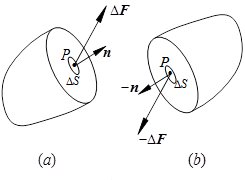
\includegraphics[width=0.3\linewidth]{pic/2013-07-30-01}
\end{center}

\pp
\begin{center}
 面积元 $\Delta S$  $\xmapsto[\text{应力张量}]{\text{$P$处应力分布}}$ 作用力 $\Delta F$.
\end{center}

\pp
若将面积元和作用力视为空间向量,则应力张量为三维空间的一个\blue{线性变换}.
\pp

通过选定三维空间的一个(直角)坐标系,则应力张量可表示为一个$3$阶方阵.
\begin{center}
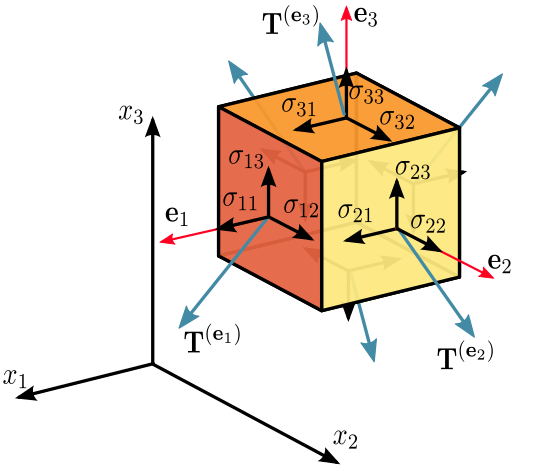
\includegraphics[width=0.2\linewidth]{pic/Components_stress_tensor}
\end{center}
\end{frame}



\subsection{本课程中的张量*}

\subsubsection{线性代数(B1)课程中学到的张量*}
\begin{frame}\frametitle{线性代数(B1)课程中学到的张量*}
给定域$\bF$上的一个线性空间$V$. 设$P$为从基$e=(e_1,\cdots,e_n)$到基$e'=(e'_1,\cdots,e'_n)$的过渡矩阵.
\pp
即
\[(e'_1,\cdots,e'_n)=(e_1,\cdots,e_n)P \qquad \text{或}\qquad  \blue{e'_j = \sum_{i=1}^{n} e_i \cdot (P)^i_j}.\]
其中任意矩阵$A$,记$(A)^i_j$为$A$的第$i$行$j$列的元素. 对于任意列向量$X$,记$(X)^i$为$X$的第$i$个元素.
\pp

\bigskip
\begin{enumerate}
\item 线性空间$V$中的向量;  	\hfill{($(1,0)$-型张量)}
\pp
\begin{center}
$V$中向量 $\xrightarrow[v=(e_1,\cdots,e_n)X]{\text{$V$的一组基}}$   坐标 + 坐标变换公式(逆变)
\end{center}
\pp
\[X' = P^{-1}X \qquad \text{或}\qquad  \blue{(X')^i = \sum_{j=1}^{n} (X)^j\cdot (P^{-1})^i_j}\]
\pp

\item 线性空间$V$上的线性变换; \hfill{($(1,1)$-型张量)}
\pp
\begin{center}
线性变换  $\xrightarrow[\sA e =e A]{\text{$V$的一组基}}$  基下矩阵 + 相似变换公式
\end{center}
\pp
\[A'=P^{-1}AP \qquad \text{或}\qquad  \blue{(A')^i_j = \sum_{s=1}^n\sum_{t=1}^n (A)^s_t\cdot (P^{-1})^i_s\cdot (P)^t_j}\]
\end{enumerate}

\end{frame}






\begin{frame}\frametitle{线性代数(B1)课程中学到的张量*}

\begin{enumerate}\setcounter{enumi}{2}
\item 若$\bF=\bR$, 空间$V$上的内积; \hfill{($(0,2)$-型张量)}
\pp
\begin{center}
内积  $\xrightarrow[G:=(g_{ij})_{n\times n}=((e_i,e_j))_{n\times n}]{\text{$V$的一组基}}$  度量矩阵 + 合同变换公式
\end{center}
\pp
\[G'=P^TGP \qquad \text{或}\qquad  \blue{g'_{ij} = \sum_{s=1}^n\sum_{t=1}^n g_{st}\cdot (P)^s_i\cdot (P)^t_j}\]

\bigskip

\item 线性空间$V$的对偶空间中的向量; \hfill{($(0,1)$-型张量)}
\pp
\begin{center}
$V^*$中向量  $\xrightarrow[Y = (f(e_1),\cdots,f(e_n))]{\text{$V$的一组基}}$   对偶基下的坐标 + 坐标变换公式(协变)
\end{center}
\pp
\[Y'=YP \qquad \text{或}\qquad  \blue{(Y')_j = \sum_{i=1}^n (Y)_i\cdot (P)^i_j}.\]
\end{enumerate}
\end{frame}


\subsection{张量的数学理解*}


\subsubsection{(物理学中的)张量在数学上的理解*}
\begin{frame}\frametitle{(物理学中的)张量在数学上的理解*}
从$n$维线性空间$V$出发,通过某些方法构造出一些其他线性空间. 这些线性空间中的向量都称为$V$上的张量.
\pp
例如
\begin{enumerate}
\item 逆变张量 \hfill{$V$}
\pp
\item 协变张量 \hfill{$V^*$}
\pp
\item $(p,q)$-型张量  \hfill{$V^{p,q}:=\underbrace{V\otimes\cdots\otimes V}_{p\text{个}} \otimes \underbrace{V^*\otimes\cdots\otimes V^*}_{q\text{个}}$}
\begin{itemize}
\pp
\item $r$阶(逆变)张量 \hfill $V^{\otimes r}=V^{r,0}=\underbrace{V\otimes\cdots\otimes V}_{r\text{个}}$
\pp
\item  $(1,1)$-型张量  \hfill{$V\otimes V^* \cong \mathrm{Hom}(V,V)$}
\end{itemize}
\pp
\item $r$-阶对称张量 ($r\geq0$) \hfill{$\mathrm{Sym}^r(V)\subset V^{\otimes r}$}
\pp
\item $r$-阶反对称张量($0\leq r\leq n$) \hfill{$\bigwedge^r(V)\subset V^{\otimes r}$}
\pp
\item $(p,q)$-型赝张量 \hfill $V^{p,q}\otimes \bigwedge^n(V)$
\begin{itemize}
\pp
\item 赝标量 \hfill $\bigwedge^n(V)$
\pp
\item 赝矢量 \hfill $V\otimes \bigwedge^n(V)$
\end{itemize}
\end{enumerate}
\pp

\blue{注:} 在这里仅考虑(仿射)线性空间上的张量. 若在欧式空间上我们有自然的同构$V^*\cong V$, $V^{p,q}\cong V^{\otimes(p+q)}$, $V\otimes\bigwedge^nV\cong\bigwedge^{n-1}V$等.
\pp

接下来,我们将通过张量积来定义这些空间.
\end{frame}



\subsection{线性空间张量积*}

\subsubsection{线性空间张量积的非严谨定义*}
\begin{frame}\frametitle{线性空间张量积的非严谨定义*}
\begin{proposition}[张量积的一种简单描述]
设$e_1,\cdots,e_m$为$V$的一组基,以及$\eta_1,\cdots,\eta_n$为$W$的一组基.
\pp
则
\begin{enumerate}
\item \blue{张量积$V\otimes W$} 是以
\[\{e_i\otimes \eta_j\mid 1\leq i \leq m, 1\leq j \leq n\}\]
为一组基的线性空间.
\pp
\item (线性性) 对于任意$v=\sum\limits_{i=1}^{m}a_ie_i\in V$和$w=\sum\limits_{j=1}^{n} b_j\eta_j\in W$, 都有
\[v\otimes w = \sum_{i=1}^{m} \sum_{j=1}^{n} a_ib_j \cdot (e_i\otimes\eta_j)\in V\otimes W.\]
\end{enumerate}
\end{proposition}
\pp

\begin{center}
\begin{tabular}{c|cccc}
 & $\eta_1$  & $\eta_2$ & $\cdots$ & $\eta_n$ \\ \hline
 $e_1$ & $e_1\otimes\eta_1$ &$e_1\otimes\eta_2$  & $\cdots$ & $e_1\otimes\eta_n$ \\
 $e_2$ & $e_2\otimes\eta_1$ &$e_2\otimes\eta_2$  & $\cdots$ & $e_2\otimes\eta_n$ \\
 $\vdots$ &  $\vdots$ &  $\vdots$ &  $\ddots$ &  $\vdots$ \\
$e_m$ & $e_m\otimes\eta_1$ &$e_m\otimes\eta_2$  & $\cdots$ & $e_m\otimes\eta_n$  \\
\end{tabular}
\end{center}
\pp

缺点: 看不出不依赖于基的选取;符号$e_i\otimes \eta_j$的意义;为什么线性?
\end{frame}



\subsection{表象与并矢*}


\subsubsection{张量积的表象,以及并矢*}
\begin{frame}\frametitle{张量积的表象,以及并矢*}
从上述描述可看出,当取定线性空间$V$和$W$的一组基后,这两个线性空间的张量积中的元素(称为\blue{张量})可以用一个矩阵表达.
\pp
我们有
\begin{center}
\[V\otimes W \xrightarrow[1:1]{\text{取定$V$和$W$的一组基}} \bF^{m\times n}\]
\end{center}
\pp

\begin{definition}[二阶张量的另一种写法(并矢)]
设$V$和$W$是有限维$F$-线性空间.\pp
对于任意 $v\in V$, $w\in W$,也称它们的张量积 $v\otimes w \in V\otimes W$为 $v$ 和 $w$的\blue{并矢积},记为 \blue{$vw$}.
\pp
称并矢积的线性组合(即 $V\otimes W$中的元素)为\blue{并矢张量}.
\end{definition}
\pp
注: 取定$V$的一组基后,并矢积对应于秩一矩阵,而并矢张量可对应于任意矩阵。
\end{frame}



\subsection{欧式空间上的张量积*}

\subsubsection{欧式空间上的张量积(非严谨定义)*}
\begin{frame}\frametitle{欧式空间上的张量积(非严谨定义)*}
若 $V$和$W$为欧氏空间(或酉空间),则$V\otimes W$上可如下定义一个内积
\[(v_1\otimes w_1,v_2\otimes w_2) := (v_1,v_2)\times (w_1,w_2).\tag{$*$}\]
\pp

\begin{proposition} 设$V$和$W$为两欧氏(酉)空间.则$V\otimes W$也为欧氏(酉)空间.
\pp
若$e_1,\cdots,e_m$和$\eta_1,\cdots,\eta_n$分别为$V$和$W$的标准正交基,则
\[\{e_i\otimes\eta_j\mid 1\leq i\leq m, 1\leq j\leq n\}\]
为$V\otimes W$的一组标准正交基.
\end{proposition}
\pp

\def\up{\lvert\uparrow\rangle}
\def\dn{\lvert\downarrow\rangle}

\begin{example}
设$V_1$,$V_2$为二维酉空间. 设$\lvert\uparrow\rangle_i$和$\dn_i$为$V_i$($i=1,2$)的标准正交基.
\pp
记
\begin{equation*}
\begin{split}
\up_1\up_2 & :=\up_1\otimes\up_2,\quad \dn_1\up_2  :=\dn_1\otimes\up_2,\\ \up_1\dn_2 & :=\up_1\otimes\dn_2, \quad
\dn_1\dn_2  :=\dn_1\otimes\dn_2.\\
\end{split}
\end{equation*}
\pp
则$\up_1\up_2$, $\dn_1\up_2$, $\up_1\dn_2$, $\dn_1\dn_2$构成$V_1\otimes V_2$的一组标准正交基.
\end{example}
\end{frame}



\subsection{多个线性空间张量积*}

\subsubsection{多个线性空间的张量积的非严谨定义*}
\begin{frame}\frametitle{多个线性空间的张量积的非严谨定义*}
\begin{proposition}[多个线性空间张量积]
设$V_1,V_2\cdots,V_r$为有限维$\bF$-线性空间,维数分别为$n_1,n_2,\cdots,n_r$.
\pp
设$\{e_{ij_i}\mid j_i=1,\cdots,n_i\}$为$V_i$的一组基.
\pp
\begin{enumerate}
\item \blue{张量积$V_1\otimes \cdots \otimes V_r$} 定义为以\\
$\quad \{e_{1,j_1}\otimes e_{2,j_2} \otimes \cdots \otimes e_{r,j_r} \mid 1\leq i \leq r, 1\leq j_i \leq \dim(V_i)\}$\\
为一组基的线性空间.
\pp
\item (线性的) 对所有的$i\in \{1,\cdots,r\}$,任取$v_i=\sum_{j_i=1}^{n_i} a_{ij_i} e_{ij_i}\in V_i$, 有
\[\blue{v_1\otimes v_2\otimes \cdots \otimes v_r} = \sum_{j_1=1}^{n_1} \cdots  \sum_{j_r=1}^{n_r} a_{1j_1} \cdots a_{rj_r} (e_{1j_1}\otimes \cdots\otimes e_{rj_r}).\]
\end{enumerate}
\end{proposition}
\pp

\def\up{\lvert\uparrow\rangle}
\def\dn{\lvert\downarrow\rangle}
\begin{example}
设$V_1$,$V_2,V_3$为二维酉空间. 设$\up_i$和$\dn_i$为$V_i$($i=1,2,3$)的标准正交基. 则$\up_1\up_2\up_3$, $\up_1\up_2\dn_3$, $\up_1\dn_2\up_3$,$\up_1\dn_2\dn_3$,$\dn_1\up_2\up_3$, $\dn_1\up_2\dn_3$, $\dn_1\dn_2\up_3$,$\dn_1\dn_2\dn_3$构成$V_1\otimes V_2\otimes V_3$的标准正交基.
\end{example}
\end{frame}



\subsection{张量及其表象*}


\subsubsection{张量(数、向量与线性变换的高阶推广)*}
\begin{frame}\frametitle{张量(数、向量与线性变换的高阶推广)*}
\begin{enumerate}
\item $V_1\otimes \cdots \otimes V_r$ 中的元素称为\blue{张量}. \pp 张量\footnote{不是所以的张量都能写成$v_1\otimes \cdots \otimes v_r$的形式.}的一般形式为
\[\sum_{j_1=1}^{n_1}\sum_{j_2=1}^{n_2}\cdots \sum_{j_r=1}^{n_r} a_{j_1,\cdots,j_r} \left( e_{1,j_1}\otimes e_{2,j_2} \otimes \cdots \otimes e_{r,j_r}\right).\] \pp
\item 对于每个线性空间$V_i$固定一组基$\{e_{ij}\mid j=1,\cdots,n_i\}$, 则张量通过其系数阵列表示出来: \pp
\begin{enumerate}
\item 当$r=0$时,一个张量就可表示为一个数; \pp
\item 当$r=1$时,一个张量就可表示为一个$n_1$维数组向量; \pp
\item 当$r=2$时,一个张量就可表示为一个$n_1\times n_2$阶的矩阵 $(a_{ij})_{n_1\times n_2}$; \pp
\item 当$r=3$时,一个张量就可表示为一个由数组成的$n_1\times n_2\times n_3$阶三维阵列$(a_{j_1,j_2,j_3})_{n_1\times n_2\times n_3}$;\pp
\item 当$r=4$时,一个张量就可表示为一个由数组成的$n_1\times n_2\times n_3\times n_4$阶四维阵列$(a_{j_1,j_2,j_3,j_4})_{n_1\times n_2\times n_3\times n_4}$.\pp
\item $\cdots$
\end{enumerate}
\end{enumerate}
\pp
注:张量虽然可以用坐标系统来表达为数(标量)的阵列,但张量本身仅仅为张量积中的一个向量,并不依赖于基(参照系)的选择.\\
\pp

我们称这个高维阵列为张量在给定\blue{基下的表象}.下面将考虑表象在不同基下的变换.
\end{frame}





\subsubsection{张量在不同基下表象之间的关系.*}
\begin{frame}\frametitle{张量在不同基下表象之间的关系.*}

\begin{definition}
设$V_1,V_2\cdots,V_r$为有限维$\bF$-线性空间,维数分别为$n_1,n_2,\cdots,n_r$.
\pp
设$\{e_{ij_i}\mid j_i=1,\cdots,n_i\}$为$V_i$的一组基.
\pp
若
\[T = \sum_{j_1=1}^{n_1}\sum_{j_2=1}^{n_2}\cdots \sum_{j_r=1}^{n_r} a_{j_1,\cdots,j_r} \left( e_{1,j_1}\otimes e_{2,j_2} \otimes \cdots \otimes e_{r,j_r}\right).\]
则称$r$维阵列$(a_{j_1,\cdots,j_r})$为$T$的在基$\{e_{ij_i}\mid j_i=1,\cdots,n_i\}$($i=1,\cdots,r$)下的\blue{表象}.
\end{definition}
\pp

\begin{equation*}
\xymatrix@C=2cm@R=0mm{
\bF^{n_1\times n_2\times \cdots \times n_r}  & V_1\otimes \cdots \otimes V_r \ar[r]^{\text{$V_i$的基} e_{i1},e_{i2},\cdots,e_{in_i}}_{1:1} \ar[l]_{\text{$V_i$的基} e'_{i1},e'_{i2},\cdots,e'_{in_i}}^{1:1} &  \bF^{n_1\times n_2\times \cdots \times n_r} \\
(a'_{i_1\cdots i_r})_{n_1\times \cdots \times n_r} & T  \ar@{|->}[r]\ar@{|->}[l] &
(a_{i_1\cdots i_r})_{n_1\times \cdots \times n_r}
}
\end{equation*}

\end{frame}





\begin{frame}\frametitle{张量在不同基下表象之间的关系.*}

\begin{equation*}
\begin{split}
T & = \sum_{j_1=1}^{n_1}\sum_{j_2=1}^{n_2}\cdots \sum_{j_r=1}^{n_r} a_{j_1,\cdots,j_r} \left( e_{1,j_1}\otimes e_{2,j_2} \otimes \cdots \otimes e_{r,j_r}\right) \\
  & = \sum_{j_1=1}^{n_1}\sum_{j_2=1}^{n_2}\cdots \sum_{j_r=1}^{n_r} a'_{j_1,\cdots,j_r} \left( e'_{1,j_1}\otimes e'_{2,j_2} \otimes \cdots \otimes e'_{r,j_r}\right) \\
\end{split}
\end{equation*}
\pp

\bigskip

\begin{theorem}
设从基$e_{i1},e_{i2},\cdots,e_{in_i}$到基$e'_{i1},e'_{i2},\cdots,e'_{in_i}$的过渡矩阵为$P_i$.
\pp
即
 \[(e'_{i1},e'_{i2},\cdots,e'_{in_i}) = (e_{i1},e_{i2},\cdots,e_{in_i})P_i\]
或者 $e_{ij_i} = \sum_{j'_i}^{n_i} e'_{ij'_i} (P_i^{-1})^{j'_i}_{j_i}$.
\pp
则
\blue{\[a'_{j'_1j'_2\cdots j'_r} = \sum_{j_1=1}^{n_1}\sum_{j_2=1}^{n_2}\cdots \sum_{j_r=1}^{n_r} a_{j_1j_2\cdots j_r} \cdot (P_1^{-1})^{j'_1}_{j_1} \cdot (P_2^{-1})^{j'_2}_{j_2} \cdots (P_r^{-1})^{j'_r}_{j_r}.\]}
其中对任意矩阵$A$,记$(A)^i_j$为矩阵$A$的第$i$行第$j$列的元素.
\end{theorem}

\end{frame}



\subsection{$(p,q)$-型张量*}

\subsubsection{$(p,q)$-型张量*}
\begin{frame}\frametitle{$(p,q)$-型张量*}
设$V$为有限维$\bF$-线性空间.记
\[V^{p,q}:= \underbrace{V\otimes\cdots\otimes V}_{p\text{个}}\otimes\underbrace{V^*\otimes\cdots\otimes V^*}_{q\text{个}}.\]
\pp
称向量空间$V^{p,q}$中的向量为$V$上的\blue{$(p,q)$-型张量}.
\pp
\begin{lemma}
任取$V$的一组基 $e_1,\cdots,e_n$. 则我们在其对偶空间上有典则的对偶基
\[f_1,\cdots,f_n,\]
以及$V^{p,q}$上也有典则的一组基
\[\{e_{i_1}\otimes e_{i_2}\otimes \cdots \otimes e_{i_p}\otimes f_{j_1}\otimes f_{j_2}\otimes \cdots \otimes f_{j_q} \mid 1\leq i_1,\cdots,i_p,j_1,\cdots,j_q\leq n\}.\]
\end{lemma}
\pp
任意 $(p,q)$-型张量$T$可唯一地表示为:
\[T = \sum_{i_1=1}^{n}\cdots\sum_{i_p=1}^{n} \sum_{j_1=1}^{n}\cdots\sum_{j_q=1}^{n} a^{i_1,\cdots,i_p}_{j_1,\cdots,j_q} \cdot e_{i_1}\otimes e_{i_2}\otimes \cdots \otimes e_{i_p}\otimes f_{j_1}\otimes f_{j_2}\otimes \cdots \otimes f_{j_q}.\]
\pp
此时,$T$在基$e_1,\cdots,e_n$下的表象为$(p+q)$维阵列
\[\blue{(a^{i_1,\cdots,i_p}_{j_1,\cdots,j_q})} \in \bF^{n\times \cdots\times n\times n\times \cdots\times n}.\]
\pp

下面我们将考虑这一表象如何随着基的选取来变动.
\end{frame}





\subsubsection{$(p,q)$-型张量在不同基下的表象之间的关系*}
\begin{frame}\frametitle{$(p,q)$-型张量在不同基下的表象之间的关系*}
设$(e'_1,\cdots,e'_n)=(e_1,\cdots,e_n)P$为$V$另一组基. 则这组基的对偶基$(f'_1,\cdots,f'_n)$满足
\[(f'_1,\cdots,f'_n)=(f_1,\cdots,f_n)(P^{-1})^T.\]

记 $P^i_j$和$(P^{-1})^i_j$分别为矩阵$P$和$P^{-1}$的第$i$行第$j$列的元素. 若$T$在基$e'_1,\cdots,e'_n$下的表象为$(p+q)$维阵列$({a'}^{i'_1,\cdots,i'_p}_{j'_1,\cdots,j'_q})$. 即,
\begin{equation*}
\begin{split}
T &= \sum_{i_1=1}^{n}\cdots\sum_{i_p=1}^{n} \sum_{j_1=1}^{n}\cdots\sum_{j_q=1}^{n} a^{i_1,\cdots,i_p}_{j_1,\cdots,j_q} \cdot e_{i_1}\otimes e_{i_2}\otimes \cdots \otimes e_{i_p}\otimes f_{j_1}\otimes f_{j_2}\otimes \cdots \otimes f_{j_q}\\
&= \sum_{i'_1=1}^{n}\cdots\sum_{i'_p=1}^{n} \sum_{j'_1=1}^{n}\cdots\sum_{j'_q=1}^{n} a^{i'_1,\cdots,i'_p}_{j'_1,\cdots,j'_q} \cdot e'_{i'_1}\otimes e'_{i'_2}\otimes \cdots \otimes e'_{i'_p}\otimes f'_{j'_1}\otimes f'_{j'_2}\otimes \cdots \otimes f'_{j'_q}\\
\end{split}
\end{equation*}
\pp
\begin{theorem}
\blue{
\begin{equation*}
{a'}^{i'_1,\cdots,i'_p}_{j'_1,\cdots,j'_q} = \sum_{i_1=1}^{n}\cdots\sum_{i_p=1}^{n} \sum_{j_1=1}^{n}\cdots\sum_{j_q=1}^{n} a^{i_1,\cdots,i_p}_{j_1,\cdots,j_q} \cdot (P^{-1})_{i_1}^{i'_1}\cdots (P^{-1})_{i_p}^{i'_p} \cdot (P)_{j'_1}^{j_1}\cdots (P)_{j'_q}^{j_q}
\end{equation*}
}
\end{theorem}

\end{frame}





\subsection{对称张量积*}


\subsubsection{对称张量积的非严谨定义*}
\begin{frame}\frametitle{对称张量积的非严谨定义*}
\begin{proposition}[对称张量积]
设$V$为$n$维$\bF$-线性空间.设$\{e_{1},\cdots,e_n\}$为$V$的一组基.
\begin{enumerate}
\item \blue{线性空间$V$的$r$阶张量积$\mathrm{Sym}^r(V)$} 是以
\[ \{e_{i_1}\odot e_{i_2} \odot \cdots \odot e_{i_r} \mid 1\leq i_1\leq i_2\leq \cdots \leq i_r\leq n\}\]
为一组基的线性空间.
\item (对称性) 对 $i_1,i_2,\cdots,i_r$的任意其他排序$i_{\sigma(1)},i_{\sigma(2)},\cdots,i_{\sigma(r)}$, 有
\[e_{i_{\sigma(1)}}\odot e_{i_{\sigma(2)}} \odot\cdots\odot e_{i_{\sigma(r)}}=e_{i_1}\odot e_{i_2} \odot \cdots \odot e_{i_r};\]
\item (线性性) 对所有的$i\in \{1,\cdots,r\}$,任取$v_i=\sum_{j_i=1}^{n} a_{ij_i} e_{j_i}\in V$, 有
\[\blue{v_1\odot v_2\odot \cdots \odot v_r} = \sum_{j_1=1}^{n} \cdots  \sum_{j_r=1}^{n} a_{1j_1} \cdots a_{rj_r} (e_{j_1}\odot \cdots\odot e_{j_r}).\]
\end{enumerate}
\end{proposition}
\pp
\begin{center}
\begin{tabular}{c|cccc}
 $\mathrm{Sym}^2(V)$& $e_1$  & $e_2$ & $\cdots$ & $e_n$ \\ \hline
 $e_1$ & $e_1\odot e_1$ &$e_1\odot e_2$  & $\cdots$ & $e_1\odot e_n$ \\
 $e_2$ &  &$e_2\odot e_2$  & $\cdots$ & $e_2\odot e_n$ \\
 $\vdots$ &   &   &  $\ddots$ &  $\vdots$ \\
$e_n$ &  &  & & $e_n\odot e_n$  \\
\end{tabular}
\end{center}
\end{frame}





\subsubsection{对称张量积的一种理解办法*}
\begin{frame}\frametitle{对称张量积的一种理解办法*}
\begin{proposition}
设$V$为$n$维线性空间.设$X_1,\cdots,X_n\in V$为$V$的一组基. 考虑以$X_1,\cdots,X_n$为变元的$r$-次齐次多项式组成的空间 $\bF[X_1,\cdots,X_n]_r$. 则
\[V = \bF[X_1,\cdots,X_n]_1,\]
以及
\[\mathrm{Sym}^rV \cong \bF[X_1,\cdots,X_n]_r.\]
\end{proposition}

\end{frame}





\subsubsection{对称张量积$\mathrm{Sym}(V)$与张量积$V^{\otimes r}$之间的关系*}
\begin{frame}\frametitle{对称张量积$\mathrm{Sym}(V)$与张量积$V^{\otimes r}$之间的关系*}
记$V^{\otimes r}:=\underbrace{V\otimes \cdots \otimes V}_{r\text{次}}$.
\pp
我们可以定义如下线性单射
\begin{equation*}
\xymatrix@R=0mm{
\mathrm{Sym}(V) \ar[r] & V^{\otimes r}\\
v_1\odot v_2\odot \cdots \odot v_r \ar@{|->}[r]
& \frac1{r!}\sum\limits_{\sigma\in S_r} v_{\sigma(1)}\otimes v_{\sigma(2)} \otimes \cdots \otimes v_{\sigma(r)} \in V^{\otimes r}
}
\end{equation*}
\pp

于是$\mathrm{Sym}^r(V)$可看成由``对称的张量''组成的$V^{\otimes r}$的子空间\\
\[\mathrm{Sym}^r(V)\subset V^{\otimes r}\]
\pp
\footnote{通过上述线性单射,我们将$v_1\odot v_2\odot \cdots \odot v_r$ 和
$\frac1{r!}\sum\limits_{\sigma\in S_r} v_{\sigma(1)}\otimes v_{\sigma(2)} \otimes \cdots \otimes v_{\sigma(r)} \in V^{\otimes r}$ 等同起来. 例如: $v\odot v = v\otimes v$, $v\odot w = \frac{v\otimes w + w\otimes v}{2}$, $v\odot v\odot v = v\otimes v \otimes v$
{\footnotesize
\begin{equation*}
v\odot w\odot u =\frac{v\otimes w \otimes u + v\otimes u \otimes w + w\otimes v \otimes u +  w\otimes u \otimes v +u\otimes v \otimes w + u\otimes w \otimes v }{6}.
\end{equation*}}
}

\end{frame}





\subsubsection{对称张量的表象*}
\begin{frame}\frametitle{对称张量的表象*}
取定$V$的一组基$e_1,\cdots,e_n$,任取
\[T = \sum_{i_1=1}^{n}\sum_{i_2=1}^{n}\cdots\sum_{i_r=1}^{n} a_{i_1,i_2,\cdots,i_r} \cdot e_{i_1}\otimes e_{i_2}\otimes \cdots \otimes e_{i_r}\in V^{\otimes r}.\]
\pp
即 $(a_{i_1,i_2,\cdots,i_r})$为张量$T\in V^{\otimes r}$在基$e_1,\cdots,e_n$下的表象.
\pp
\begin{proposition}
张量$T$落在子空间$\mathrm{Sym}^rV$中,当且仅当对任意$1\leq i_1,i_2,\cdots,i_r\leq n$以及任意$1\leq s<t\leq r$ ,有
\[a_{i_1,\cdots,i_s,\cdots,i_t,\cdots,i_r} = a_{i_1,\cdots,i_t,\cdots,i_s,\cdots,i_r}\]
\end{proposition}

\pp

\begin{example}
$(2,0)$-型张量$T$对称当且仅当其对应矩阵为对称矩阵.
\end{example}
\end{frame}





\subsection{反对称张量积*}

\subsubsection{反对称张量积的非严谨定义*}
\begin{frame}\frametitle{反对称张量积的非严谨定义*}
\begin{proposition}[反对称张量积]
设$V$为$n$维$\bF$-线性空间.设$\{e_{1},\cdots,e_n\}$为$V$的一组基.
\begin{enumerate}
\item \blue{线性空间$V$的$r$阶张量积$\bigwedge^r(V)$} 是以
\[ \{e_{i_1}\wedge e_{i_2} \wedge \cdots \wedge e_{i_r} \mid 1\leq i_1< i_2< \cdots < i_r\leq n\}\]
为一组基的线性空间.
\item (反对称性) 对任意$1\leq i_1,i_2,\cdots,i_r\leq n$,
\begin{equation*}
e_{i_1}\wedge e_{i_2} \wedge \cdots \wedge e_{i_r}:=
\left\{
\begin{array}{ll}
(-1)^{\tau(\sigma)} e_{i_{\sigma(1)}}\wedge e_{i_{\sigma(2)}} \wedge\cdots\wedge e_{i_{\sigma(r)}}& \text{两两不同.}\\
0 & \text{其他};\\
\end{array}
\right.
\end{equation*}
其中$i_{\sigma(1)},i_{\sigma(2)},\cdots,i_{\sigma(r)}$为从小到大的排序.
\item (线性性) 对所有的$i\in \{1,\cdots,r\}$,任取$v_i=\sum_{j_i=1}^{n} a_{ij_i} e_{j_i}\in V$, 则
\[\blue{v_1\wedge v_2\wedge \cdots \wedge v_r} = \sum_{j_1=1}^{n} \cdots  \sum_{j_r=1}^{n} a_{1j_1} \cdots a_{rj_r} (e_{j_1}\wedge \cdots\wedge e_{j_r}).\]
\end{enumerate}
\end{proposition}

注: 线性空间$\bigwedge^rV$的维数为 ${n\choose r}$. 特别地, $\bigwedge^0 V= \bF$ 和 $\bigwedge^nV$都为$1$维线性空间. 前者中的元素被称为\blue{标量},而后者中的元素被称为\blue{赝标量}.

\end{frame}






\subsubsection{反对称张量积$\bigwedge^r(V)$与张量积$V^{\otimes r}$之间的关系*}
\begin{frame}\frametitle{反对称张量积$\bigwedge^r(V)$与张量积$V^{\otimes r}$之间的关系*}
我们可以定义如下线性单射
\begin{equation*}
\xymatrix@R=0mm{
\bigwedge^rV \ar[r] & V^{\otimes r}\\
v_1\wedge v_2\wedge \cdots \wedge v_r \ar@{|->}[r]
& \frac1{r!}\sum\limits_{\sigma\in S_r} (-1)^{\tau(\sigma)} v_{\sigma(1)}\otimes v_{\sigma(2)} \otimes \cdots \otimes v_{\sigma(r)} \in V^{\otimes r}
}
\end{equation*}

于是$\bigwedge^r(V)$可看成由``反对称的张量''组成的$V^{\otimes r}$的子空间\footnote{通过上述线性单射,我们将$v_1\wedge v_2\wedge \cdots \wedge v_r$ 和
$\frac1{r!}\sum\limits_{\sigma\in S_r} (-1)^{\tau(\sigma)} v_{\sigma(1)}\otimes v_{\sigma(2)} \otimes \cdots \otimes v_{\sigma(r)} \in V^{\otimes r}$ 等同起来. 例如: $v \wedge v = 0$, $v \wedge w = \frac{v\otimes w - w\otimes v}{2}$, $v\wedge v\wedge v =0$
{\footnotesize
\begin{equation*}
v\wedge w\wedge u =\frac{v\otimes w \otimes u - v\otimes u \otimes w - w\otimes v \otimes u +  w\otimes u \otimes v + u\otimes v \otimes w - u\otimes w \otimes v }{6}.
\end{equation*}}}\\

\[\bigwedge^r V\subset V^{\otimes r}\]

\end{frame}





\subsubsection{反对称张量的表象*}
\begin{frame}\frametitle{反对称张量的表象*}
取定$V$的一组基$e_1,\cdots,e_n$,任取
\[T = \sum_{i_1=1}^{n}\sum_{i_2=1}^{n}\cdots\sum_{i_r=1}^{n} a_{i_1,i_2,\cdots,i_r} \cdot e_{i_1}\otimes e_{i_2}\otimes \cdots \otimes e_{i_r}\in V^{\otimes r}.\]
即 $(a_{i_1,i_2,\cdots,i_r})$为张量$T\in V^{\otimes r}$在基$e_1,\cdots,e_n$下的表象.
\begin{proposition}
张量$T$落在子空间$\bigwedge^rV$中,当且仅当对任意$1\leq i_1,i_2,\cdots,i_r\leq n$以及任意$1\leq s<t\leq r$ ,有
\[a_{i_1,\cdots,i_s,\cdots,i_t,\cdots,i_r} = - a_{i_1,\cdots,i_t,\cdots,i_s,\cdots,i_r}\]
\end{proposition}
\begin{example}
$(2,0)$-型张量$T$反对称当且仅当其对应矩阵为反对称矩阵.
\end{example}
\end{frame}



\subsection{赝张量*}



\subsubsection{$(p,q)$-型赝张量*}
\begin{frame}\frametitle{$(p,q)$-型赝张量*}

设$V$为$n$维$\bF$-线性空间. 则$\bigwedge^n V$为$1$维线性空间,称其中的向量为\blue{赝标量}.
\pp
记
\[V^{p,q}\otimes \bigwedge^n V:= \underbrace{V\otimes\cdots\otimes V}_{p\text{个}}\otimes\underbrace{V^*\otimes\cdots\otimes V^*}_{q\text{个}}\otimes \bigwedge^n V.\]
\pp
称向量空间$V^{p,q}\otimes \bigwedge^n V$中的向量为$V$上的\blue{$(p,q)$-型赝张量}.

\pp
特别地, $V\otimes \bigwedge^n V$ 中的向量称为\blue{赝矢量}.
\end{frame}





\subsubsection{赝标量的表象*}
\begin{frame}\frametitle{赝标量的表象*}

\begin{definition}
设$V$为$n$维$\bF$-线性空间.
\pp
任取$V$的一组基$e_1,\cdots,e_n$, 则$1$维线性空间$\bigwedge^n V$存在典范基$e_1\wedge e_2\wedge \cdots \wedge e_n$.
\pp
称$a$为赝标量$T\in \bigwedge^n V$在基$e_1,\cdots,e_n$下的\blue{表象},若
\[T = a \cdot e_1\wedge e_2\wedge \cdots \wedge e_n.\]
\end{definition}
\pp

\begin{proposition}
若$(e'_1,\cdots,e'_n)=(e_1,\cdots,e_n)P$为$V$的另一组基.
\pp
设$a'$为$T$在基$e'_1,\cdots,e'_n$下的表象.
\pp
则
\[a' = \det(P)^{-1}\cdot a.\]
\end{proposition}
\pp

\begin{corollary}
\begin{itemize}
\item 若$P$为第一类正交矩阵,则$a'$和$a$相等.
\pp
\item 若$P$为第二类正交矩阵,则$a'$和$a$相差一个符号.
\pp
\item 特别地,若交换一组基中的两个向量的位置,则赝标量对应的表象将改变符号.
\end{itemize}
\end{corollary}

\end{frame}


\subsection{张量场*}


\subsubsection{张量场及其上的微积分*}
\begin{frame}\frametitle{张量场及其上的微积分*}

向量场

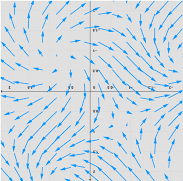
\includegraphics[width=0.4\linewidth]{pic/vector field}

\pp

\bigskip

切空间

\pp
\bigskip

张量场(例如余切向量场(即一阶微分形式),应力张量场等)

\bigskip

\pp

标量场(函数)
\end{frame}



\subsection{严谨定义*}

\subsubsection{严谨定义*}
\begin{frame}\frametitle{严谨定义*}
上述非严谨的定义中,需要固定各线性空间的一组基。而数学和物理中通常希望一个量或者一个概念不依赖于基(坐标系、参考系)的选取。这要求我们内蕴地给出张量积的定义。

\bigskip

在给出严谨定义之前,我们需要引入一些基本概念。
\begin{itemize}
\item 线性函数与对偶空间
\item 多重线性映射(函数)
\end{itemize}
\end{frame}





\subsubsection{Hom空间,线性函数与对偶空间*}
\begin{frame}\frametitle{Hom空间,线性函数与对偶空间*}
设$V$和$W$为有限维$\bF$-线性空间.\pp 从$V$到$W$上的全体线性映射组成的集合记为
\[\blue{\mathrm{Hom}(V,W)} = \{\mA \colon V\rightarrow W\mid \mA \text{为线性映射}\}.\]
\pp
称从$V$到$\bF$的线性映射为$V$上的线性函数.\pp 记
\[\blue{V^*} = \mathrm{Hom}(V,\bF) = \{f\colon V\rightarrow \bF\mid f \text{为线性函数}\}.\]

\pp
\bigskip

在$\mathrm{Hom}(V,W)$以及$V^*$上,按如下方式定义加法和数乘
\begin{equation*}
\begin{split}
& (\blue{f+g})(v) := f(v) + g(v) \\
& (\blue{\lambda f})(v) := \lambda f(v) \\
\end{split}
\end{equation*}
\pp
\begin{proposition}
在上述加法和数乘下, $\mathrm{Hom}(V,W)$ 和 $V^*$均构成$\bF$-线性空间.\pp 称后者为$V$的\blue{对偶空间}.
\end{proposition}
\end{frame}





\subsubsection{对偶空间基本性质*}
\begin{frame}\frametitle{对偶空间基本性质*}

\begin{proposition}[对偶空间的维数与基]
\begin{itemize}
\item 对偶空间$V^*$的维数与$V$的维数相同.\pp
\item 若$e_1,\cdots,e_n$为$V$的一组基,则$V^*$存在唯一的一组基$f_1,\cdots,f_n$满足
\[f_j(e_i)=\delta_{ij}=\left\{{1, \quad \text{若 }i=j;\atop 0,\quad \text{若 }i\neq j}\right..\]\pp
称$f_1,\cdots,f_n$为$e_1,\cdots,e_n$的\blue{对偶基}.
\end{itemize}
\end{proposition}
\pp
我们有如下自然的\blue{取值映射(evaluation map)}:
\[ev\colon V^*\times V\rightarrow \bF; \quad (f,v)\mapsto f(v).\]
\pp
\begin{proposition}
\[ V\cong V^{**} \quad v \mapsto ev(-,v) \]
\end{proposition}
\pp
注: 若我们不要求$V$为有限维的,则映射$V\rightarrow V^{**}$仅为单射.
\end{frame}





\subsubsection{向量的逆变性与对偶向量的协变性*}
\begin{frame}\frametitle{向量的逆变性与对偶向量的协变性*}

\begin{proposition}[向量的逆变性与对偶向量的协变性]
设$e_1,\cdots,e_n$以及 $e'_1,\cdots,e'_n$为$V$为有限维$\bF$-线性空间的两组基.设过渡矩阵为 $A$,即
\[(e'_1,\cdots,e'_n) = (e_1,\cdots,e_n)\blue{A}.\]
记这两组基的对偶基分别为$f_1,\cdots,f_n$和$f'_1,\cdots,f'_n$.
\begin{enumerate}
\item (向量的逆变性) 设$v\in V$在两组基下坐标为$X$和$X'$. 即,
\[v = (e_1,\cdots,e_n)X = (e'_1,\cdots,e'_n)X'.\]
则
\[\blue{X' = A^{-1}X} \quad \text{或} \quad \blue{(x'_1,\cdots,x'_n) = (x_1,\cdots,x_n) (A^{-1})^T}.\]
\item (对偶向量协变性) 设对偶向量$f$在两组对偶基下坐标为$Y$和$Y'$.即,
\[f  = (f_1,\cdots,f_n)Y = (f'_1,\cdots,f'_n)Y'.\]
则
\[\blue{Y' = A^TY}  \quad \text{或} \quad \blue{(y'_1,\cdots,y'_n) = (y_1,\cdots,y_n)A}.\]
\end{enumerate}
\end{proposition}
\yang{证明思路:\[(f'_1,\cdots,f'_n) = (f_1,\cdots,f_n) (A^T)^{-1}.\]}
\end{frame}





\subsubsection{多重线性映射*}
\begin{frame}\frametitle{多重线性映射*}
设 $V_1,V_2,\cdots,V_r,W$为有限维$\bF$-线性空间.\pp 若映射
\[\tau \colon V_1\times V_2\times \cdots \times V_r \rightarrow W\]
对每个分量都是线性的, 即对所有的指标$i=1,2,\cdots,r$,都有
\begin{equation*}
{\small{
\tau(v_1,\cdots,\alpha v_i + \beta v'_i,\cdots,v_r) = \alpha \tau(v_1,\cdots,v_i,\cdots,v_r) + \beta \tau(v_1,\cdots,v'_i,\cdots,v_r),}}
\end{equation*}
则称$\tau$为从$V_1\times V_2\times \cdots \times V_r$到$W$的\blue{多重线性映射}.\pp 特别地,若$W=\bF$,则称多重线性映射
\[\tau \colon V_1\times V_2\times \cdots \times V_r \rightarrow \bF\]
为$V_1\times V_2\times \cdots \times V_r$上的\blue{多重线性函数}.
\end{frame}





\subsubsection{多重线性映射例子*}
\begin{frame}\frametitle{多重线性映射例子*}
\begin{example}[行列式]
行列式$\det \colon \bF^n \times \bF^n \times \cdots \times \bF^n \longrightarrow \bF$为多重线性函数.
\end{example}
\pp
\begin{example}[取值映射]
取值映射$ ev \colon V^*\times V\rightarrow \bF$是双线性函数.
\end{example}

\begin{example}[三维空间的点积]
\[-\cdot- \colon \bR^3\times\bR^3 \rightarrow \bR;\]
\[(a_1,a_2,a_3)\cdot(b_1,b_2,b_3)=a_1b_1+a_2b_2+a_3b_3.\]
\end{example}

\begin{example}[三维空间的叉积]
\[-\times- \colon \bR^3\times\bR^3 \rightarrow \bR^3\]
\[(a_1,a_2,a_3)\times(b_1,b_2,b_3) = (a_2b_3-a_3b_2,a_3b_1-a_1b_3,a_1b_2-a_2b_1).\]
\end{example}

\end{frame}





\subsubsection{多重线性映射组成的空间*}
\begin{frame}\frametitle{多重线性映射组成的空间*}
我们如下定义多重线性映射的加法和数乘.\pp 任取从$V_1\times V_2\times \cdots \times V_r$到$W$的两个多重线性映射$\tau$和$\tau'$,以及$\lambda\in\bF$,
\begin{equation*}
\begin{split}
& (\blue{\tau+\tau'})(v_1,v_2,\cdots,v_n):= \tau(v_1,v_2,\cdots,v_n) + \tau'(v_1,v_2,\cdots,v_n); \\
& (\blue{\lambda\tau})(v_1,v_2,\cdots,v_n):= \lambda\cdot \tau(v_1,v_2,\cdots,v_n).
\end{split}
\end{equation*}
\pp
\begin{proposition}
从$V_1\times V_2\times \cdots \times V_r$到$W$的全体多重线性映射组成的集合在上述加法和数乘下构成$\bF$-线性空间.
\end{proposition}

\end{frame}





\subsubsection{两线性空间的张量积严谨定义*}
\begin{frame}\frametitle{两线性空间的张量积严谨定义*}
设$V$和$W$为两有限维$\bF$-线性空间.
\pp
\begin{definition}[张量积的无坐标化严谨定义]
称线性空间 $\blue{V\otimes W}:=\{\tau \colon V^*\times W^* \rightarrow \bF \mid \tau \text{为双线性函数}\}$
为$V$和$W$的\blue{张量积}.
\end{definition}
\pp
任取$v\in V$以及$w\in W$, 如下定义从$V^*\times W^*$到$\bF$函数
\[(f,g)\mapsto f(v)g(w).\]
则这一函数为双线性的,记为 $\blue{v\otimes w} \in V\otimes W$.
\pp
\begin{proposition}
设$e_1,\cdots,e_m$为$V$的一组基,以及$\eta_1,\cdots,\eta_n$为$W$的一组基.则
\[\{e_i\otimes \eta_j\mid 1\leq i \leq m, 1\leq j \leq n\}\]
为张量积$V\otimes W$的一组基.
\end{proposition}
\pp
\begin{proposition}[张量运算关于分量的线性性]
\[(\alpha v+\beta v')\otimes w =\alpha (v\otimes w) + \beta (v'\otimes w) \in V\otimes W.\]
\[v\otimes(\alpha w+\beta w') =\alpha (v\otimes w) + \beta (v\otimes w') \in V\otimes W.\]
\end{proposition}
\end{frame}

%\subsubsection{什么是向量*}
%\begin{frame}\frametitle{张量积的泛性质(张量积在范畴论中的定义)*}
%\pp
%\begin{proposition}[张量积泛性质]
%\begin{enumerate}
%\item 张量运算 $(v,w)\mapsto v\otimes w$为从$V\times W$到$V\otimes W$的双重线性映射;\pp
%\item 对于任意$\bF$-线性空间$U$,存在如下一一对应
%\[\{f\colon V\times W \rightarrow U \mid f \text{双线性}\} \xleftrightarrow[f=g\circ h]{\quad 1:1 \quad } \{g \colon V\otimes W \rightarrow U\mid g \text{线性}\}\]
%\end{enumerate}
%\end{proposition}
%\end{frame}





\subsubsection{多个线性空间的张量积的严谨定义*}
\begin{frame}\frametitle{多个线性空间的张量积的严谨定义*}
设$V_1,\cdots,V_r$为有限维$\bF$-线性空间.
\pp
\begin{definition}
记$\blue{V_1\otimes \cdots \otimes V_r} :=\{\tau \colon V_1^*\times \cdots \times V_r^* \rightarrow \bF \mid \tau \text{为多重线性函数}\}$. 称这一线性空间为有限维$\bF$-线性空间$V_1,\cdots,V_r$的\blue{张量积},其中的向量均称为\blue{张量}.
\end{definition}
\pp
如下定义$\blue{v_1\otimes \cdots \otimes v_r} \in V_1\otimes \cdots \otimes V_r$:
\[v_1\otimes \cdots \otimes v_r\colon (f_1,\cdots,f_r)\mapsto f_1(v_1)\cdots f_r(v_r).\]
\pp
\begin{proposition}
设$\{e_{ij}\mid j=1,\cdots,n_i\}$为$V_i$的一组基.\pp 则
\[\{e_{1,j_1}\otimes e_{2,j_2} \otimes \cdots \otimes e_{r,j_r} \mid 1\leq i \leq r, 1\leq j_i \leq \dim(V_i)\}\]
为$V_1\otimes \cdots \otimes V_r$的一组基.
\end{proposition}
\end{frame}





\subsubsection{$(p,q)$-型张量*}
\begin{frame}\frametitle{$(p,q)$-型张量*}
设$V$为有限维$\bF$-线性空间.记
\[V^{p,q}:= \underbrace{V\otimes\cdots\otimes V}_{p\text{个}}\otimes\underbrace{V^*\otimes\cdots\otimes V^*}_{q\text{个}}.\]
称向量空间$V^{p,q}$中的向量为$V$上的\blue{$(p,q)$-型张量}.

\begin{lemma}
设$U,V,W$为三个有限维$\bF$-线性空间.则存在如下典范映射
\[ V\cong V\otimes\bF\cong \mathrm{Hom}(\bF,V)\cong \mathrm{Hom}(V^*,\bF),\]
和
\[\mathrm{Hom}(U\otimes V^*,W)\cong\mathrm{Hom}(U,V\otimes W).\]
\end{lemma}

\end{frame}





\subsubsection{$(p,q)$-型张量*}
\begin{frame}\frametitle{$(p,q)$-型张量*}

\begin{theorem}设$V$为有限维$\bF$-线性空间. 则以下三个线性空间之间存在典范同构
\begin{itemize}
\item $\underbrace{V\otimes\cdots\otimes V}_{p\text{个}}\otimes\underbrace{V^*\otimes\cdots\otimes V^*}_{q\text{个}}$
\item $\mathrm{Hom}_{\bF}(\underbrace{V\otimes\cdots\otimes V}_{q\text{个}},\underbrace{V\otimes\cdots\otimes V}_{p\text{个}})$
\item $\mathrm{Hom}_{\bF}\big(\underbrace{V^*\otimes\cdots\otimes V^*}_{p\text{个}}\otimes\underbrace{V\otimes\cdots\otimes V}_{q\text{个}},\bF\big)$
\item 多重线性函数$\phi\colon \underbrace{V^*\times\cdots\times V^*}_{p\text{个}}\times\underbrace{V\times\cdots\times V}_{q\text{个}} \rightarrow \bF$组成的空间.
\end{itemize}
这些空间中的向量都可称为\blue{$(p,q)$-型张量}.
\end{theorem}
\end{frame}





\subsubsection{对称张量积的严谨定义*}
\begin{frame}\frametitle{对称张量积的严谨定义*}
设$V$为有限维$\bF$-线性空间. 设$\tau \colon \underbrace{V^*\times \cdots \times V^*}_{r\text{个}} \rightarrow \bF$为$r$-重线性函数.我们称其为\blue{对称的},若对于任意$1\leq i<j\leq r$以及任意$f_1,f_2,\cdots,f_r\in V^*$, 都有
\[\tau(f_1,\cdots,f_i,\cdots,f_j,\cdots,f_r)=\tau(f_1,\cdots,f_j,\cdots,f_i,\cdots,f_r).\]
\pp
\begin{definition}
记$\blue{\mathrm{Sym}^r(V)} :=\{\tau \colon \underbrace{V^*\times \cdots \times V^*}_{r\text{个}} \rightarrow \bF \mid \tau \text{为对称的$r$重线性函数}\}$. 则这是$V^{\otimes r}$的一个子空间. 称之$V$的\blue{$r$阶对称张量积}.
\end{definition}
\pp
定义
\[v_1\odot v_2\odot \cdots \odot v_r := \frac1{r!}\sum\limits_{\sigma\in S_r} v_{\sigma(1)}\otimes v_{\sigma(2)} \otimes \cdots \otimes v_{\sigma(r)} \in V^{\otimes r}\]
\pp
\begin{proposition}
设$e_1,\cdots,e_n$为$V$的一组基.\pp 则
\[ \{e_{i_1}\odot e_{i_2} \odot \cdots \odot e_{i_r} \mid 1\leq i_1\leq i_2\leq \cdots \leq i_r\leq n\}\]
为$\mathrm{Sym}^r(V)$一组基.
\end{proposition}
\end{frame}





\subsubsection{外积与反对称张量的严谨定义*}
\begin{frame}\frametitle{外积与反对称张量的严谨定义*}
设$V$为有限维$\bF$-线性空间. 设$\tau \colon \underbrace{V^*\times \cdots \times V^*}_{r\text{个}} \rightarrow \bF$为$r$-重线性函数.我们称其为\blue{反对称的},若对于任意$1\leq i<j\leq r$以及任意$f_1,f_2,\cdots,f_r\in V^*$, 都有
\[\tau(f_1,\cdots,f_i,\cdots,f_j,\cdots,f_r)=\blue{-}\tau(f_1,\cdots,f_j,\cdots,f_i,\cdots,f_r).\]
\pp
\begin{definition}
记$\blue{\bigwedge^r(V)} :=\{\tau \colon \underbrace{V^*\times \cdots \times V^*}_{r\text{个}} \rightarrow \bF \mid \tau \text{为反对称的$r$重线性函数}\}$. 则这是$V^{\otimes r}$的一个子空间. 称之$V$的\blue{$r$阶反对称张量积}.
\end{definition}
\pp
定义
\[v_1\wedge v_2\wedge \cdots \wedge v_r := \frac1{r!}\sum\limits_{\sigma\in S_r} (-1)^{\tau(\sigma)} v_{\sigma(1)}\otimes v_{\sigma(2)} \otimes \cdots \otimes v_{\sigma(r)} \in V^{\otimes r}\]
\pp
\begin{proposition}
设$e_1,\cdots,e_n$为$V$的一组基.\pp 则
\[ \{e_{i_1}\wedge e_{i_2} \wedge \cdots \wedge e_{i_r} \mid 1\leq i_1<i_2<\cdots <i_r\leq n\}\]
为$\bigwedge^r(V)$一组基.
\end{proposition}
\end{frame}





\subsubsection{张量的缩并*}
\begin{frame}\frametitle{张量的缩并*}

设$p,q$为正整数.对于任意给定$1\leq i\leq p$和$1\leq j\leq q$,我们有如下缩并映射
\[\Phi^i_j\colon V^{(p,q)} \longrightarrow V^{(p-1,q-1)}\]
其将 $v_1\otimes \cdots \otimes v_i \otimes \cdots \otimes v_p \otimes f_1\otimes \cdots \otimes f_j \otimes \cdots \otimes f_q$映成
\[ f_j(v_i) \cdot (v_1\otimes \cdots \otimes v_{i-1} \otimes v_{i+1} \otimes \cdots \otimes v_p) \otimes (f_1\otimes \cdots \otimes f_{j-1}\otimes f_{j+1}\otimes \cdots \otimes f_q)\]

\begin{proposition}
设$V$和$W$为两有限维$\bF$-线性空间.\pp 则
\begin{enumerate}
\item 存在典范同构
\[W\otimes V^*\cong\mathrm{Hom}(V,W)\]
将$w\otimes f$映成线性映射$(v \mapsto f(v)w)$.
\item 若$W=V$,则上述同构与 $\mathrm{tr}$ (迹) 的合成正好为缩并映射. 即下图交换
\begin{equation*}
\xymatrix{
V\otimes V^* \ar[dr]_{\Phi_1^1} \ar[r]^-{\cong}&  \mathrm{Hom}(V,V) \ar[d]^{\mathrm{tr}}\\
& \bF\\}
\end{equation*}
\end{enumerate}
\end{proposition}
\end{frame}









% ========== 2023年07月04号 第34次课 习题课 ==========








% ========== 2023年07月06号 第35次课 习题课 ==========










% ========== 2023年07月06号 第**次课 应用 ==========

%\frame{\titlepage}

\section{应用*}


\title{第十一章 \quad 应用*}
\author{}
\date{}

\makeatletter
\ifodd\value{page}
    \frame{\titlepage}
\else
    \frame{\mbox{}}
    \frame{\titlepage}
\fi
\makeatother



\subsection{桁架的静力分析*}
\begin{frame}\frametitle{桁架的静力分析*}

    桁架是一种由直杆铰接而成的空间结构, 杆件主要承受轴向拉力和压力. 例如:屋顶、桥梁、塔架等.

    \begin{figure}
    \centering
    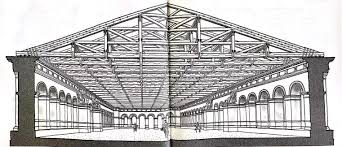
\includegraphics[width=0.3\linewidth]{pic/屋顶}
    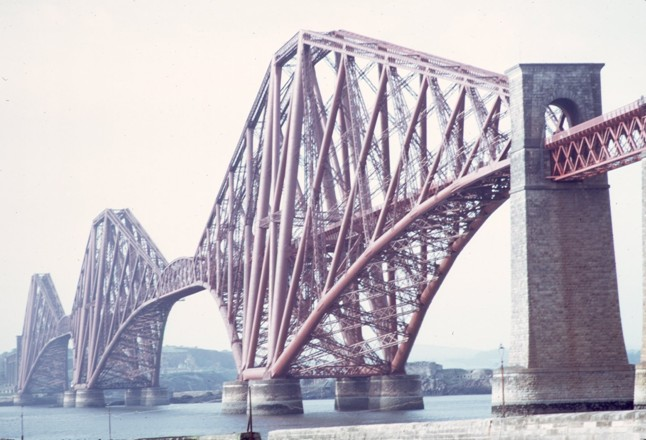
\includegraphics[width=0.3\linewidth]{pic/桥}
    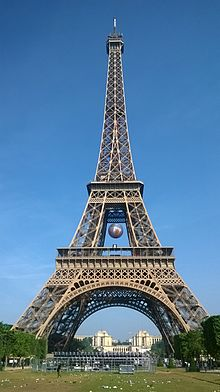
\includegraphics[width=0.3\linewidth]{pic/塔}
    \end{figure}
    \end{frame}






\begin{frame}\frametitle{桁架的静力分析*}
    \begin{question}
    考虑如下桁架的简化模型. 各个直杆长度相同,忽略桁架自重.
    在 $B$处施以一个大小为$F$的向下的力.求各个直杆所承受的力.
    \end{question}

% 定义自定义样式
\tikzset{
  line/.style={draw, thick}, % 定义线条样式
  dot/.style={circle, fill, inner sep=1.5pt}, % 定义点样式
  dot label/.style={font=\scriptsize} % 定义标签样式
}
    \begin{center}
    \begin{tikzpicture}
    \coordinate (A) at (-2,1.732);
    \coordinate (B) at (0,1.732);
    \coordinate (C) at (2,1.732);
    \coordinate (D) at (-3,0);
    \coordinate (E) at (-1,0);
    \coordinate (F) at (1,0);
    \coordinate (G) at (3,0);

    \node at (-1,1.732) [below] {$\ell_1$};
    \node at (1,1.732) [below] {$\ell_2$};
    \node at (-2.5,0.866) [right] {$\ell_3$};
    \node at (-1.5,0.866) [right] {$\ell_4$};
    \node at (-0.5,0.866) [right] {$\ell_5$};
    \node at (0.5,0.866) [right] {$\ell_6$};
    \node at (1.5,0.866) [right] {$\ell_7$};
    \node at (2.5,0.866) [right] {$\ell_8$};
    \node at (-2,0) [above] {$\ell_9$};
    \node at (0,0) [above] {$\ell_{10}$};
    \node at (2,0) [above] {$\ell_{11}$};

    \draw[line]
    (A)--(B)--(C)--(G)--(F)--(E)--(D)--(A)--(E)--(B)--(F)--(C);
    \foreach \i/\angle in {A/120,B/90,C/60,D/-120,E/-90,F/-90,G/-60} {
    \node[dot, label={[dot label]\angle:$\i$}] at (\i) {};
      }
    \end{tikzpicture}
    \end{center}
    \end{frame}






\begin{frame}\frametitle{桁架的静力分析*}
    解:记杆$\ell_i$受到大小为$f_i$的压力(压力为负,则表示受到拉力). 根据各节点处杆件的平衡条件可得
    \begin{equation*}
    \left\{\begin{array}{lll}
    (P_1):& -f_1+\frac12(f_3-f_4)=0,& f_3+f_4=0;\\
    (P_2):& f_1-f_2=0,&\frac{\sqrt{3}}{2}(f_5+f_6)=F;\\
    (P_3):& f_2+\frac12(f_7-f_8)=0,&f_7+f_8=0;\\
    (P_5):&f_4+f_5=0 &\frac12(f_4-f_5)+f_9-f_{10}=0;\\
    (P_6):&f_6+f_7=0 &\frac12(f_6-f_7)+f_{10}-f_{11}=0;\\
    (P_4,P7):&\frac12f_3+f_9=0, &\frac12f_8+f_{11}=0\\
    \end{array}\right.
    \end{equation*}
    \end{frame}





\subsection{电网络分析*}
\begin{frame}\frametitle{电网络分析*}
    \begin{question}
    考虑如下RLC电路图.已知 $R_1=1\Omega$, $R_2=3\Omega$, $\epsilon=3V$, $C=0.5F$, $L=5H$.设初始开关断开,各支路电流都为零.
    \begin{figure}
    \centering
    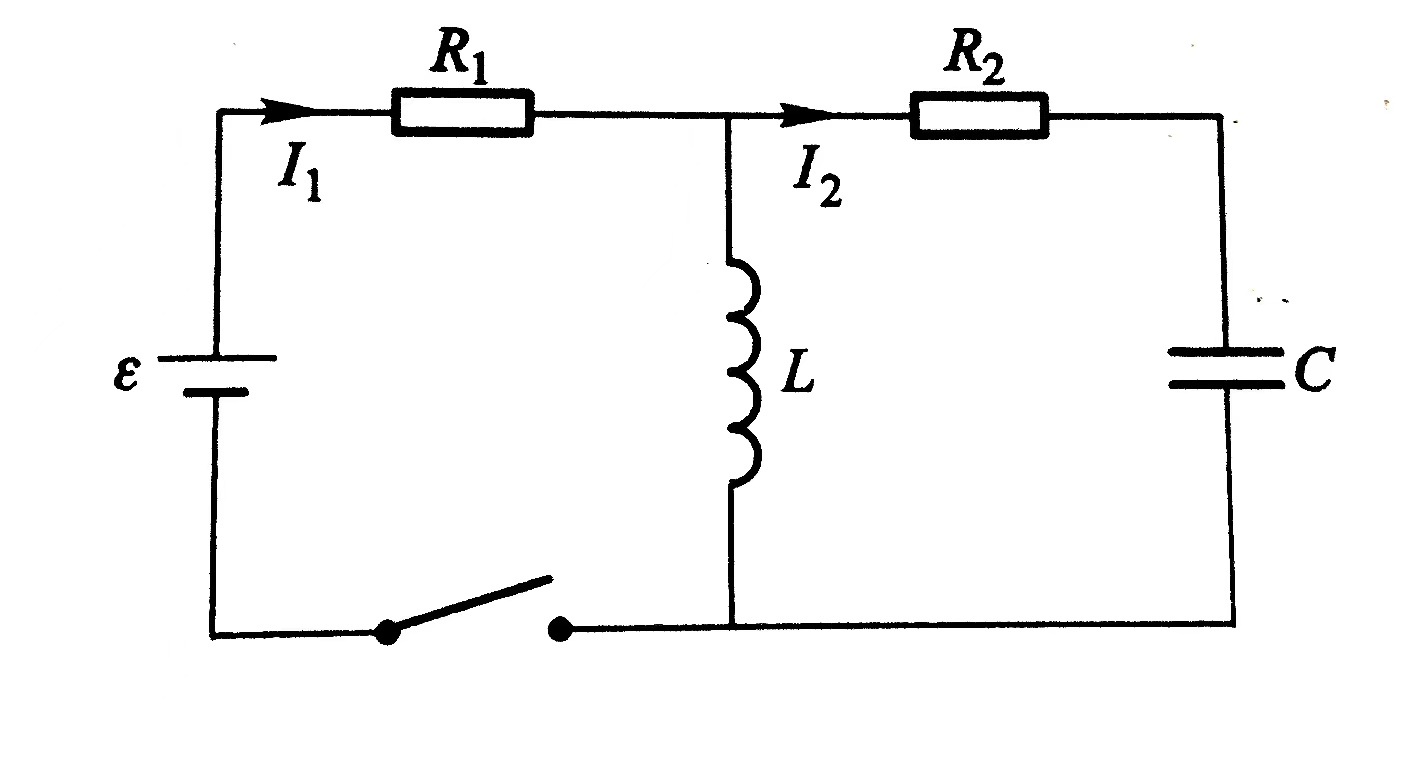
\includegraphics[width=0.4\linewidth]{pic/电路图}
    \end{figure}
    求开关闭合后两个支路的电流$I_1(t)$和$I_2(t)$随时间的变化.
    \end{question}
    解: 根据Krichhoff定律和Phm定律,可得微分方程组:
    \begin{equation*}
    \left\{
    \begin{array}{l}
    L(I_1(t)-I_2(t))' = \epsilon - R_1I_1(t)\\
    C(\epsilon-R_1I_1(t)-R_2I_2(t))' = I_2(t) \\
    I_1(0) = I_2(0) = 0\\
    \end{array}
    \right.
    \end{equation*}\end{frame}






\begin{frame}\frametitle{电网络分析*}
    于是
    \begin{equation*}
    \begin{pmatrix}I_1'(t)\\I_2'(t)\\\end{pmatrix}
    =\begin{pmatrix}-\frac{3}{20}&-\frac12\\\frac1{20}&-\frac12\\\end{pmatrix}
    \begin{pmatrix}I_1(t)-3\\I_2(t)\\\end{pmatrix}
    \end{equation*}
    解得
    \[\begin{pmatrix}I_1(t)-3\\I_2(t)\\\end{pmatrix} = e^{At}\begin{pmatrix}-3\\0\\\end{pmatrix}\]
    其中
    \[A=\begin{pmatrix}-\frac{3}{20}&-\frac12\\\frac1{20}&-\frac12\\\end{pmatrix}
    =\begin{pmatrix}2&5\\1&1\\\end{pmatrix} \begin{pmatrix}-\frac25&\\&-\frac14\\\end{pmatrix}\begin{pmatrix}2&5\\1&1\\\end{pmatrix}^{-1}\]
    \[e^{At}=\sum_{n=0}^{\infty}\frac{t^n}{n!}A^n=\begin{pmatrix}2&5\\1&1\\\end{pmatrix} \begin{pmatrix}e^{-\frac{2t}5}&\\&e^{-\frac{t}4}\\\end{pmatrix}\begin{pmatrix}2&5\\1&1\\\end{pmatrix}^{-1}\]
    从而,得
    \begin{equation*}
    \left\{
    \begin{array}{l}
    I_1(t) = 3 +2e^{-\frac{2t}{5}} - 5e^{-\frac{t}{4}}\\
    I_2(t) = e^{-\frac{2t}{5}} - e^{-\frac{t}{4}}\\
    \end{array}
    \right.
    \end{equation*}
    \end{frame}





    \subsection{多项式公因子与方程求解*}
\begin{frame}\frametitle{多项式公因子与方程求解*}
    给定两个一元多项式
    \[f(x)=a_0+a_1x+\cdots+a_mx^m,\quad g(x)=b_0+b_1x+\cdots+b_nx^n,\quad (a_mb_n\neq0).\]
    \begin{question}
    在不做因式分解和不求这两个多项式的根的情况下,如何判断它们是否有公因子或公共根?
    \end{question}
    称方阵 $S=\begin{pmatrix}
    a_0 &&& b_0&&\\
    a_1 &\ddots&& b_1&\ddots&\\
    \vdots &\ddots&a_0& \vdots&\ddots&b_0\\
    a_m &&a_1& b_m&&b_1\\
     &\ddots&\vdots&&\ddots& \vdots\\
    &&a_m&&&b_m\\
    \end{pmatrix} $
    为$f(x)$和$g(x)$的Sylvester矩阵.称其行列式$Syl(f,g):=\det(S)$为Sylvester结式.
    \begin{theorem}
    多项式$f(x)$和$g(x)$有公因子,当且仅当$\det(S)=0$.
    \end{theorem}
    \end{frame}






\begin{frame}\frametitle{多项式公因子与方程求解*}
    证明思路:这是由于$f(x)$和$g(x)$有公因子,当且仅当存在非零多项式$A(x)=A_0+A_1x+\cdots+A_{n-1}x^{n-1}$和$B(x)=B_0+B_1x+\cdots+B_{m-1}x^{m-1}$使得
    \[A(x)f(x)+B(x)g(x)=0\qquad(**)\]
    计算$(**)$中的系数得
    \[\begin{pmatrix}
    a_0 &&& b_0&&\\
    a_1 &\ddots&& b_1&\ddots&\\
    \vdots &\ddots&a_0& \vdots&\ddots&b_0\\
    a_m &&a_1& b_m&&b_1\\
     &\ddots&\vdots&&\ddots& \vdots\\
    &&a_m&&&b_m\\
    \end{pmatrix}
    \begin{pmatrix}A_0\\\vdots\\A_{n-1}\\B_0\\\cdots\\B_{m-1}\\\end{pmatrix}=0\qquad(***)\]
    而齐次方程$(***)$有解当且仅当$\det(S)=0$.
    \end{frame}





    \subsection{组合与图论*}
\begin{frame}\frametitle{组合与图论*}
    \begin{question}
    假设 $m$个学生组织了 $n$次集体活动, 每次至少 $2$人参加, 并且任意 $2$个同学一起参加的活动恰有 $1$次. 求证: $n=1$或者$m\leq n$.
    \end{question}
    解: 令 $A=(a_{ij})_{m\times n}$, 其中若学生$i$参加了活动$j$则$a_{ij}=1$,否则$a_{ij}=0$. 由题意知
    \[AA^T = \begin{pmatrix} t_1 & 1&\cdots&1\\1&t_2&\ddots&\vdots\\\vdots&\ddots&\ddots&1\\1&\cdots&1&t_m\\\end{pmatrix}_.\]
    其中$t_i$为学生$i$参加活动总次数.

    分情况讨论:
    \begin{itemize}
    \item 若 $t_i=1$,则 $n=1$;
    \item 若对所有$i$,$t_i\geq2$.则 $AA^T>0$.因此$A$行满秩,从而$m\leq n$.
    \end{itemize}
    \end{frame}






\begin{frame}\frametitle{组合与图论*}
    \begin{question}[关灯游戏]
    在$m\times n$的棋盘中每个方格内均设置一盏灯和一个按钮. 当某个方格内的按钮被按动后,这个方格内的灯将从亮变灭或从灭变亮,与这个方格有公共边的方格内的灯也将同样的变化.假设初始时每盏灯都是亮的,问是否可以按下一些列的按钮使得最终所有灯都变灭.
    \end{question}
    解题思路: 灯的状态可用$\mathbb F_2^N$中的向量代表.每个按钮也都看成$\mathbb F_2^N$中的一个向量$\alpha_i$.则问题转化为判定
    $\textbf{1}=(1,1,\cdots,1)^T$是否落在$\{\alpha_1,\cdots,\alpha_{mn}\}$生成子空间$V$中.

    令$A=(\alpha_1,\cdots,\alpha_{mn})$,则 $A$对称且对角线全为$1$. 从而
    \[y^TAy =\textbf{1}^Ty.\]
    因此与$V$正交的向量都与$\textbf{1}$正交. 从而$\textbf{1}\in V$. 也就是说可以经过一些列的按钮使得最终所有灯都变灭.

    \bigskip

    注: 组合数学和图论中的许多问题都可以转化为矩阵问题处理.
    \end{frame}





    \subsection{多元函数的极值*}
\begin{frame}\frametitle{多元函数的极值*}
    设$\textbf{x}=(x_1,\cdots,x_n)$是$n$个变量, $f(\textbf{x})$是定义在区域$D\subseteq R^n$上的$n$元光滑函数.根据Taylor公式
    \[f(\textbf{x}) = f(\textbf{a}) +J(\textbf{a})(\textbf{x}-\textbf{a}) + \frac12(\textbf{x}-\textbf{a})^T\textbf{H}(\textbf{a})(\textbf{x}-\textbf{a})+o(|\textbf{x}-\textbf{a}|^2),\]
    其中
    \[J(\textbf{x}) = \left(\frac{\partial f(\textbf{x})}{\partial x_1},\cdots,\frac{\partial f(\textbf{x})}{\partial x_n}\right)\qquad \text{Jacobi 矩阵}\]
    和
    \[H(\textbf{x}) = \begin{pmatrix}
    \frac{\partial^2 f(\textbf{x})}{\partial x^2_1} & \cdots & \frac{\partial^2 f(\textbf{x})}{\partial x_1\partial x_n}\\
    \vdots&&\vdots\\
    \frac{\partial^2 f(\textbf{x})}{\partial x_n\partial x_1} & \cdots & \frac{\partial^2 f(\textbf{x})}{\partial x_n^2}\\
    \end{pmatrix} \qquad \text{Hesse 矩阵}.\]

    \begin{theorem}假设同上. 则有
    \begin{itemize}
    \item 设 $f(x)$ 在 $\textbf{a}$ 处达到极小(大)值, 则$J(\textbf{a}) =0$且$H(\textbf{a})\geq0(\leq0)$.
    \item 若$J(\textbf{a}) =0$且$H(\textbf{a})>0(<0)$,则$f(x)$ 在 $\textbf{a}$ 处达到极小(大)值.
    \end{itemize}
    \end{theorem}
    \end{frame}





    \subsection{计算机绘图与图像变换*}
\begin{frame}\frametitle{计算机绘图与图像变换*}
    在计算机中,无论是二维平面图形还是三维立体图形,都需要通过图形变换,把图形变换到显示器屏幕上,然后显示出来.
    \begin{figure}
    \centering
    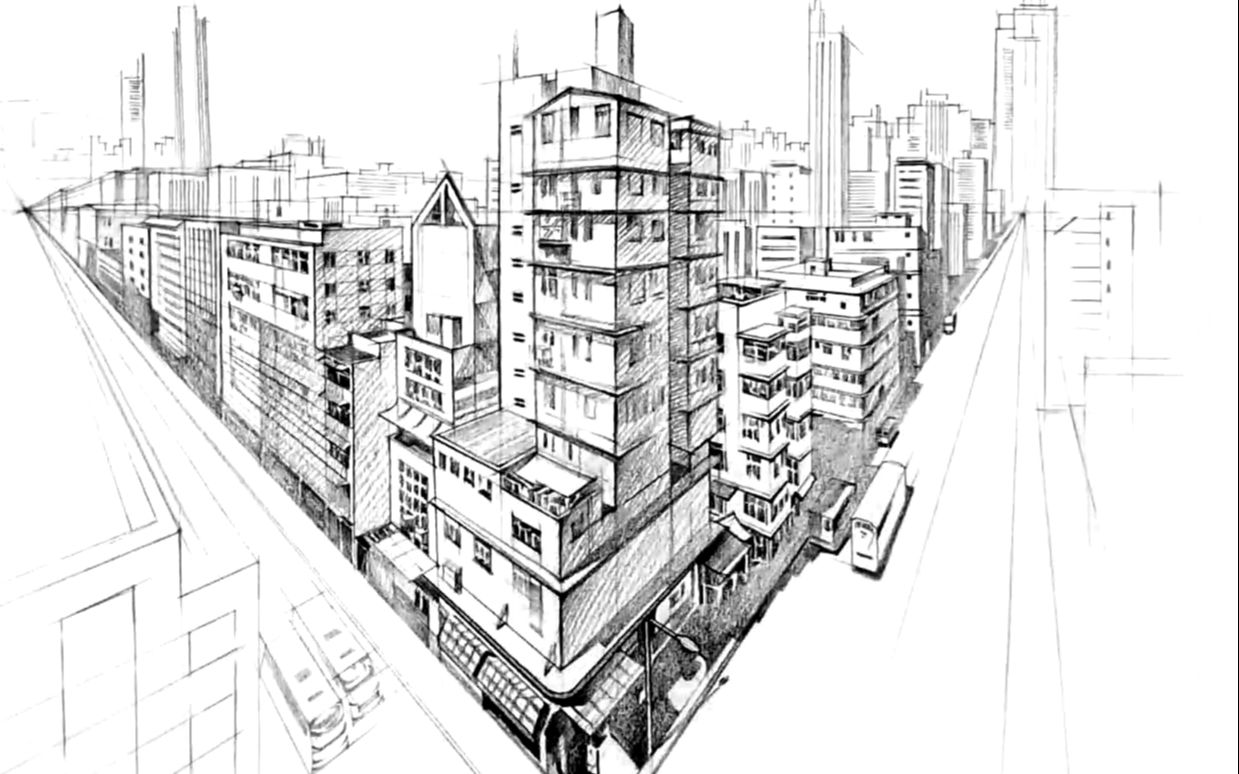
\includegraphics[width=0.4\linewidth]{pic/城市}
    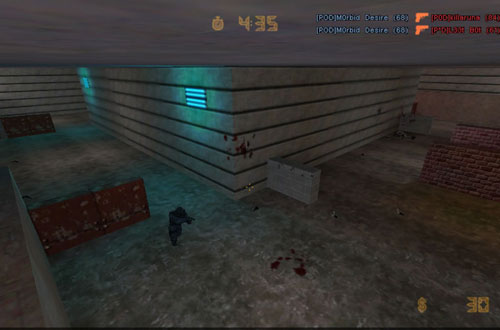
\includegraphics[width=0.4\linewidth]{pic/CS}
    \end{figure}

    二维图形变换矩阵表示
    \begin{equation*}
    \begin{pmatrix}x'\\y'\\\end{pmatrix}=
    \begin{pmatrix}a_{11}&a_{12}\\a_{21}&a_{22}\\\end{pmatrix}
    \begin{pmatrix}x\\y\\\end{pmatrix}+\begin{pmatrix}b_1\\b_2\\\end{pmatrix}
    \end{equation*}
    或者将上式齐次化表示为
    \begin{equation*}
    \begin{pmatrix}x'\\y'\\1\\\end{pmatrix}=
    \begin{pmatrix}
    a_{11}&a_{12}&b_{1}\\
    a_{21}&a_{22}&b_{2}\\
    0&0&1\\
    \end{pmatrix}
    \begin{pmatrix}x\\y\\1\\\end{pmatrix}
    \end{equation*}

    \blue{思考:} 旋转和平移变换分别对应那个矩阵?

    \end{frame}






\begin{frame}\frametitle{计算机绘图与图像变换*}
    相应的三维图像变换一般可表示为
    \begin{equation*}
    \begin{pmatrix}x'\\y'\\z'\\1\\\end{pmatrix}=
    \begin{pmatrix}
    a_{11}&a_{12}&a_{13}&b_{1}\\
    a_{21}&a_{22}&a_{23}&b_{2}\\
    a_{31}&a_{32}&a_{33}&b_{3}\\
    0&0&0&1\\
    \end{pmatrix}
    \begin{pmatrix}x\\y\\z\\1\\\end{pmatrix}
    \end{equation*}
    对于立体图形,为了保持立体视觉效果,需要将其恰当的投影到平面上.
    \begin{itemize}
    \item 中心投影: 例如以点$A(a,b,c)$为中心,坐标平面Oxy为投影平面. 则中心投影变换公式为
    \begin{equation*}
    \begin{pmatrix}x'\\y'\\z'\\w'\\\end{pmatrix}=
    \begin{pmatrix}
    c&0&a&0\\0&c&-b&0\\0&0&0&0\\0&0&-1&c\\
    \end{pmatrix}
    \begin{pmatrix}x\\y\\z\\w\\\end{pmatrix}
    \end{equation*}
    \item 平行投影: 沿着向量$(\alpha,\beta,\gamma)$投影到$Oxy$平面
    \begin{equation*}
    \begin{pmatrix}x'\\y'\\z'\\w'\\\end{pmatrix}=
    \begin{pmatrix}
    1&0&-\frac\alpha\gamma&0\\0&1&-\beta/\gamma&0\\0&0&0&0\\0&0&0&1\\
    \end{pmatrix}
    \begin{pmatrix}x\\y\\z\\w\\\end{pmatrix}
    \end{equation*}
    \end{itemize}

    注:这里都是用齐次坐标表示.

    \end{frame}





    \subsection{最小二乘法与奇异值分解*}
\begin{frame}\frametitle{最小二乘法与奇异值分解*}
    \begin{question}
    给定一组观测数据
    \[(x_i,y_i),\quad i=1,2,\cdots,n.\]
    寻找一个合适的函数$y=f(x)$使得函数图像尽量与观测数据贴合.
    \end{question}

    核心问题是如何用数学语言表述图像与观测数据贴合. 一种方便的策略是取 $f(x)$为不超过给定次数的多项式
    \[f(x)= a_0+a_1x+\cdots+a_{m-1}x^{m-1}\]
    使得
    \[g(a_0,a_1,\cdots,a_{m-1}):=\sum_{i=1}^n (f(x_i)-y_i)^2\]
    尽量小.基于该准则求拟合多项式$f(x)$的方法称为最小二乘法.
    \end{frame}





\begin{frame}\frametitle{最小二乘法与奇异值分解*}
    由 $\frac{\partial g}{\partial a_k}=0$, $k=0,1,\cdots,m-1$ 的到关于$a_0,a_1,\cdots,a_{m-1}$的线性方程组:
    \[AA^Ta=Ay \qquad (*)\]
    其中
    \begin{equation*}
    A=\begin{pmatrix}
    1&1&\cdots&1\\x_1&x_2&\cdots&x_n\\\vdots&\vdots&&\vdots\\x_1^{m-1}&x_2^{m-1}&\cdots&x_n^{m-1}\\
    \end{pmatrix},
    \quad
    a=\begin{pmatrix}a_0\\a_1\\\vdots\\a_{m-1}\\\end{pmatrix},
    \quad
    y=\begin{pmatrix}y_1\\y_2\\\vdots\\y_{n}\\\end{pmatrix}
    \end{equation*}

    分情况讨论:

    \begin{itemize}
    \item $n\geq m$: $AA^T>0$. 式$(*)$有唯一解.
    \item $n<m$: 对$A$进行奇异值分解. 即$A=PDQ$, 其中$P$, $Q$为正交矩阵, $D=\mathrm{diag}(\sigma_1,\cdots,\sigma_r,O_{(m-r)\times(n-r)})$(正交相抵标准形).
    \end{itemize}
    线性方程组(*)化简为
    \[DD^Tx=Dc\]
    其中$x=P^Ta$, $c=Qy$.于是$x_i = \frac{c_i}{\sigma_i}$, $i=1,2,\cdots,r$.于是
    \[a = P\left(\frac{c_1}{\sigma_1},\cdots,\frac{c_r}{\sigma_r},*\cdots,*\right)^T.\]
    特别地, $a=P\left(\frac{c_1}{\sigma_1},\cdots,\frac{c_r}{\sigma_r},0,\cdots,0\right)^T$为模长最小的解.
    \end{frame}





    \subsection{数字图像的压缩*}
\begin{frame}\frametitle{数字图像的压缩*}
    在不明显降低图像的视觉质量的基础上,jpeg格式对静止图片的压缩比一般可达$10:1\sim 50:1$.
    \begin{itemize}
    \item 分割成$8\times8$的子块 $A=(A_{ij})_{p\times q}$
    \item 离散余弦变换的 $B=PAP^T$其中$P=(p_{ij})_{8\times 8}$正交,$p_{1j}=\frac{1}{\sqrt{8}}$, $p_{ij}=\frac12\cos\frac{(i-1)(2j-1)\pi}{16}$ ($i\geq2$).
    \item 对$B_{ij}$(按某种方式)取整;
    \item 然后编码为长度不等的二进制数$c_{ij}$
    \item 最后得到编码系数矩阵$C=(c_{ij})_{p\times q}$.

    \end{itemize}
    \bigskip
    JPEG效果好在于$B_{ij}$是稀疏的. 即除了左上角少数元素除外,大多数元素绝对值都相当小.

    \bigskip
    图像压缩的基本方法: 寻找图像空间的一组基使得图像在这组基下的坐标为稀疏矩向量.
    \end{frame}





    \subsection{投入产出模型*}
\begin{frame}\frametitle{投入产出模型*}
    经济学家 Leontief 提出投入产出模型: 设经济社会中共有$n$中产品$P_1,P_2,\cdots,P_n$每生产一个单位的$P_i$需消耗$a_ij$个单位的$P_j$,矩阵$A=(a_{ij})_{n\times n}$称为消耗系数矩阵\footnote{为保可持续发展,须满足 $x \geq xA$,其中$x$为产出总量($y=xA$为投入总量).}.

    \begin{question}
    若以$f(x)=\min_{1\leq i\leq n}\frac{x_i}{y_i}$作为衡量生成效率的标准, $x$取何值时$f(x)$最大?
    \end{question}
    \yang{证明思路: 由Perron-Frobenius定理\footnote{不可拆分非负实方阵的最大模长特征值为正,重数为$1$且对应正特征向量. 不可拆分意思是不存在产品的重排使得$A$为准三角矩阵.},得$\lambda_1 x\geq xA$ 且等号成立当且仅当 $x$取对应特征向量.}
    \end{frame}





    \subsection{Markov矩阵*}
\begin{frame}\frametitle{Markov矩阵*}
    \begin{question}
    一个点在某网络中随机游走,在给定点出现的概率问题.
    \end{question}

    记从$i$点(随机)游走一步,到达$j$点的概率记为$m_{ij}$.则 $M=(m_{ij})_{n\times n}$为 Markov矩阵\footnote{满足$A(1,\cdots,1)^T=(1,1,\cdots,1)^T$的非负矩阵$A$,称为Markov矩阵.}.

    \begin{theorem} Markov矩阵$M=(m_{ij})_{n\times n}$有如下性质:
    \begin{enumerate}
    \item 若行向量$x$是$n$维概率向量,则$xM$也是$n$维概率向量.
    \item $1$是$M$的最大特征值, $n$为全$1$向量是对应的特征向量.
    \item 若对任意正整数$k$,$M^k$不可拆分,则$\lim_{k\to\infty}M^k=\textbf{1}\cdot c^T$,其中$c$为$M^T$属于$1$的特征向量.
    \end{enumerate}
    \end{theorem}
    \end{frame}





    \subsection{Google 搜索排序*}
\begin{frame}\frametitle{Google 搜索排序*}
    PageRank算法\footnote{Brin-Page 发明,并依此创立google.}根据网站内外链接的数量和质量来算网页的Pagerank.
    \begin{definition}
    \blue{假设}有$n$个网页,某网民在任意时刻都仅打开一个页面.假设他点击链接的概率是$\omega$,而关闭当前页面的概率为$1-\omega$. 在无限长时间后的某个时刻网页$P_j$被访问的概率为$p_j$就被称为是他的Pagerank.
    \end{definition}

    首先,构造邻接矩阵\footnote{$0$表示无连接,$1$表示有连接.}$A=(a_{ij})_{n\times n}$.
    Bayes 全概率公式
    \[p_j = \frac{1-\omega}{n} + \omega\sum_{i=1}^n p_i\frac{a_{ij}}{d_i}.\]
    解得 (其中 $D=\mathrm{diag}(d_1,\cdots,d_n)$, $p=(p_1,\cdots,p_n)$, $\textbf{1}=(1,\cdots,1)$)
    \[p=\frac{1-\omega}{n}\textbf{1}\left(1-\omega D^{-1}A\right)^{-1}.\]
    注: 实际问题中$n$很大,用Gauss消元法或计算逆矩阵的方法求解计算量为$O(n^3)$,几乎不可能实现.

    由于$D^{-1}A$为Markov矩阵,其特征值模都不超过$1$. 在Pagerank算法中,取 $\omega=0.85$,因此
    \[\left(1-\omega D^{-1}A\right)^{-1} = \sum_{i=0}^\infty \left(\omega D^{-1}A\right)^i.\]
    \end{frame}





\subsection{层次分析法*}
\begin{frame}\frametitle{层次分析法*}
    层次分析是决策论中一种重要的方法.

    设系统共有$m$层因素,第$k$层有$n_k$个. 第$k$层的第$i$个因素受第$k+1$层的第$j$个因素的影响程度为$p_{k,i,j}$.则目标层受方案层的影响程度可通过矩阵
    \[P = P_1P_2\cdots P_{m-1}\]
    来表示.

    注:矩阵$P_k$比较难确定.但比较矩阵\footnote{$b^{ki}_{j_1j_2}=\frac{p_{k,i,j_1}}{p_{k,i,j_2}}$} $B^{k\ell}=(b^{ki}_{j_1j_2})$比较好估计.

    \begin{enumerate}
    \item 估算$B$
    \item 求方程组$\left\{\frac{x_i}{x_j}=b_{ij},i,j=1,2,\cdots,n_{k+1}\right\}$的最小二乘解\footnote{需要用到行主对角占优矩阵的性质}.
    \item 令$P_k$的第$\ell$行为$x$.计算$P$.
    \end{enumerate}
    \begin{theorem}
    若$A$可逆,主对角占优($a_{ii}\geq\sum_{j\neq i}|a_{ij}|$)且$a_{ij}<0$($\forall i\neq j$),则$A^{-1}$的每个元素都为正数.
    \end{theorem}
    \end{frame}











\end{document}

